\documentclass[review]{elsarticle}
\usepackage{lineno,hyperref}
% package added by zhixuan, not sure whether allowed by JCP or not!
\usepackage{amsmath}
\usepackage{float}

\modulolinenumbers[5]
\journal{Journal of Computational Physics}
%%%%%%%%%%%%%%%%%%%%%%%
%% Elsevier bibliography styles
%%%%%%%%%%%%%%%%%%%%%%%
%% To change the style, put a % in front of the second line of the current style and
%% remove the % from the second line of the style you would like to use.
%%%%%%%%%%%%%%%%%%%%%%%
%% Numbered
\bibliographystyle{model1-num-names}
%% Numbered without titles
%\bibliographystyle{model1a-num-names}
%% Harvard
%\bibliographystyle{model2-names.bst}\biboptions{authoryear}
%% Vancouver numbered
%\usepackage{numcompress}\bibliographystyle{model3-num-names}
%% Vancouver name/year
%\usepackage{numcompress}\bibliographystyle{model4-names}\biboptions{authoryear}
%% APA style
%\bibliographystyle{model5-names}\biboptions{authoryear}
%% AMA style
%\usepackage{numcompress}\bibliographystyle{model6-num-names}
%% `Elsevier LaTeX' style
%\bibliographystyle{elsarticle-num}
%%%%%%%%%%%%%%%%%%%%%%%
\begin{document}
\begin{frontmatter}
\title{Integrating random choice method with SPH : a new scheme with adaptive artificial viscosity and shock capturing ability}
%\tnotetext[mytitlenote]{Can add  title note here}
%% Group authors per affiliation:
\author{Zhixuan Cao}
\author{Abani Patra \fnref{mycorrespondingauthor}}
\address{Department of Mechanical and Aerospace Engineering,The State University of New York at Buffalo, Amherst, NY, 14260-4200, USA}
\author{E. Bruce Pitman}
\address{Department of Materials Design and Innovation, The State University of New York at Buffalo, Amherst, NY, 14260-4200, USA}
%\fntext[myfootnote]{Since 1880.}
%% or include affiliations in footnotes:
%\author[mymainaddress,mysecondaryaddress]%{Elsevier Inc}
%\ead[url]{www.elsevier.com}
%\author[mysecondaryaddress]{Global Customer Service\corref{mycorrespondingauthor}}
\fntext[mycorrespondingauthor]{abani@buffalo.edu}
%\cortext[mycorrespondingauthor]{abani@buffalo.edu}
%\ead{abani@buffalo.edu}
%\address[mymainaddress]{1600 John F Kennedy Boulevard, Philadelphia}
%\address[mysecondaryaddress]{360 Park Avenue South, New York}

\begin{abstract}
Standard smoothed particle hydrodynamics (SPH) employs an artificial viscosity, defined explicitly by constant coefficients, to properly capture hydrodynamic shock waves.
Such methodology usually provides dissipation more than need and smears the discontinuities if the artificial viscosity coefficients are not tuned.
Excessively large artificial viscosity might also damp generation of turbulence by fluid instability.
We present in this article a novel SPH scheme with adaptive artificial viscosity, in which the artificial viscosity is determined implicitly based on solution of a local Riemann problem. Different from Godunov SPH (GSPH) method, which utilizing solution of local Riemann problem at an imaginary interface, the new method randomly sample the solution of Riemann problem mimicking the random choice method (RCM). One dimensional shock tube tests demonstrate several attractive features of this new scheme. First of all, it introduces less but sufficient artificial dissipation for shock capturing compared with classical SPH and GSPH. The pressure ``wiggle" around contact discontinuity, which persists in SPH results, is ameliorated by the new scheme. The new method also shows higher order of convergence than GSPH.
%when the same construction of local Riemann problem and Riemann solvers are adopted by both methods. 
Classical RCM method would lose its desirable property of low numerical dissipation when solving multi-dimensional unsteady non-linear systems. Combining of RCM with SPH overcomes the shortcoming  of classical RCM method. Three dimensional time dependent compressible Euler equations are solved by the new scheme for simulating a free jet flow, demonstrating that the desirable less dissipation property of the new scheme persists in multi-dimensional applications.
\end{abstract}
\begin{keyword}
Smoothed Particle Hydrodynamics (SPH), Random Choice Method (RCM), Riemann Solver, Artificial viscosity, Hyperbolic PDEs
\end{keyword}
\end{frontmatter}

\linenumbers
\section{Introduction}
Smoothed particle hydrodynamics (SPH) \citep{gingold1977smoothed,lucy1977numerical} is a mesh-free particle method based on Lagrangian formulation and has been widely applied to different areas in engineering and science. SPH has both advantages and disadvantages with respect to other numerical techniques. One main advantage is that it automatically adapts to following dynamic flows and arbitrary geometries. Another advantage is that it needs less programming effort to include more physics. In addition, SPH particles only interact with neighboring particles, which avoids massive global communication in parallel implementation of SPH.
Historically, SPH has difficulty in capturing discontinuities, such as shocks or contact discontinuities. Inviscid description of fluids becomes invalid at shock fronts, where specific entropy of the fluids increases through the conversion of mechanical energy into internal energy. Most SPH codes have included an artificial viscosity term explicitly, both for stabilizing the simulation and for handling shock discontinuities by dissipating local velocity differences and converting them into heat \citep{monaghan1983shock, monaghan1997sph, klapp2012strong}. Without knowing the minimum amount of dissipation for shock capturing, such methodology usually provides dissipation more than need and smears the discontinuity if the artificial viscosity coefficients are not tuned. The method of using constant artificial viscosity might also introduce spurious effects at region away from shocks, for instance, causing an unphysical damping of turbulent mixing (as shown, for example, by \citet{borgani2012hydrodynamic}) or spurious
shearing torques in rotating flows \citep{flebbe1994smoothed}. Selective application of artificial viscosity techniques, such as the time dependent viscosity \citep{morris1997switch, dolag2005turbulent} and shock-indicator-based viscosity \citep{cullen2010inviscid} have been tried for counteracting this. 
\citet{sigalotti2008adaptive} improved the standard SPH near sharp discontinuities adopting adaptive density kernel estimation (ADKE) techniques. However, the parameters for ADKE have to be tuned to the problem at hand \citep{puri2014comparison}. Hence it is hard to implement ADKE in real applications.

Besides adding dissipation explicitly, \citet{inutsuka2002reformulation} proposed an innovative approach to introduce dissipation implicitly by reformulating the SPH convolution integrals. Artificial viscosity is introduced implicitly by using iterative solution to a Riemann problem at an imaginary interface between an interacting particles pair. This method, named as Godunov SPH (GSPH), is attractive because it eliminates parameterization and hence user intervention associated with artificial viscosity coefficients. The GSPH method has been shown to be able to handle shock discontinuities \citep{inutsuka2002reformulation, cha2003implementations,iwasaki2011smoothed, puri2014approximate}, introduces less damping to turbulent mixing \citep{cha2010kelvin, borgani2012hydrodynamic} than standard SPH, and ameliorate pressure ``blips" (or ``wiggle" called by others) at the contact discontinuity \citep{borgani2012hydrodynamic}. However, the amount of dissipation introduced by GSPH is stll excessive than needs. When using a linear interpolation of the volume function, it has been shown \citep{borgani2012hydrodynamic} that the excess of diffusion, which manifests itself in the shock tube tests as a smooth transition at the rarefaction fan, is such to prevent the development of the Kelvin-Helmholtz (KH) instability.
%The development of KH instability is also significantly affected by number of neighbouring particles for cubic interpolation of the volume function.

The random choice method (RCM) was introduced by \citet{glimm1965solutions} for the construction of solutions of systems of nonlinear hyperbolic conservation laws. \citet{chorin1976random} developed the RCM as a practical computational method for solutions to one dimensional (1D) Euler equations of gas dynamics. Chorin's work was followed by numerous researchers, with applications and further improvements \citep{sod1977numerical,concus1979numerical,colella1982glimm, freistuhler1992numerical}. In essence, the solution is advanced in time by a sequence of operations that include solving of Riemann problems and a stochastic sampling of the solution. See \citep{toro2013riemann} for details. When applied to one dimensional time dependent Euler equations \citep{colella1982glimm}, diffusive errors from spatial averaging are completely eliminated and hence discontinuities, such as shocks or material interface, can be resolved as true discontinuities.
For unsteady flows in genuine two (or higher) space dimensions, however, such very desirable property of RCM do not seem to persist \citep{colella1982glimm}.
%This need to be proven ---> But at least, if the good property of preserving true discontinuity is still valid in 1D shock tube problem, it should be preserved in multiple-dimensional implementations. Because in current framework of RSPH, no matter what is the dimension of the problem, the techniques is only implemented in a one-dimensional scenario.

In this investigation, we introduce a new method, which will be referred to as RSPH in later paragraph, by integrating RCM method within framework of SPH. 
The new scheme inherits the attraction of classical RCM, introducing less but sufficient artificial viscosity and causing less smearing of discontinuities than other methods for 1D problems. Implementing of RCM within the framework of SPH only involves sampling of solutions of Riemann problem in 1D local coordinate system no matter what is the dimensionality of the problem. That is to say, no multi-dimensional coordinate is involved even for multi-dimensional problems. Thereby, the desirable property of RCM method in 1D should be retained in higher dimensional implementations within the framework of SPH. This hypothesis is confirmed by a three-dimensional (3D) free jet flow simulation. 

To summarize, RSPH has the following advantages over standard SPH:
\begin{itemize}
\item RSPH is able to capture discontinuities with less smearing.
\item The RSPH is able to adaptively adjust equivalent artificial viscosity coefficients, assigning larger artificial viscosity coefficients around the shock and small artificial viscosity coefficients otherwhere.
\item RSPH is able to alleviate pressure ``wiggle" at the contact discontinuity, a common issue in classical SPH.
\end{itemize}
Compared with GSPH, which is also based on solution of local Riemann problems, RSPH introduces less but sufficient dissipation than GSPH, especially in the region away from shocks. Such feature of RSPH is especially beneficial for simulating of scenarios involving turbulence mixing, for which excessive dissipation would suppress mixing. In addition, RSPH also shows faster convergence rate than GSPH.

The scheme of this paper is follows. We start with a brief review of standard SPH and GSPH in the second section. The RSPH is then explained in details in the third section followed by the numerical tests section, where both one 1D and 3D inviscid Euler equations (see Eq. (\ref{eq:gov-cs-rho}) - (\ref{eq:gov-cs-e}) are solved by standard SPH, GSPH and RSPH. Limitations and potential applications of RSPH are discussed in last section. 

Our investigation implements RSPH scheme in solving inviscid compressile Euler equations as the application case.  
\begin{align}
\dfrac{\partial \rho}{\partial t} + \nabla \cdot \left(\rho \textbf{v} \right) = 0 \label{eq:gov-cs-rho} \\
\dfrac{\partial \rho \textbf{v}}{\partial t} + \nabla \cdot \left(\rho \textbf{v} \textbf{v} + p\textbf{I}\right) = 0 \label{eq:gov-cs-v} \\
\dfrac{\partial \rho E}{\partial t} + \nabla \cdot \left[\left(\rho E + p \right)\textbf{v}\right] = 0 \label{eq:gov-cs-e}
\end{align}
where $\rho$ is the density, $\textbf{v}$ is the velocity, $\textbf{I}$ is a unit tensor.
$E = e + K $ is the total energy which is a summation of kinetic energy $K$ and internal energy $e$.
The system of equations is closed by equation of state (EOS) for idea gas.
\begin{equation}
p = \left(\gamma - 1\right)\rho e \label{eq:EOS}
\end{equation}
with $\gamma=1.4$.

For any SPH scheme, governing equations in Lagrange form are needed. By deducting kinetic energy from energy equation, subtracting mass conservation from momentum equation, combining transient term and advection term into material derivative (for any function $A$, material derivative is defined as $\frac{D A}{Dt} = \frac{\partial A}{\partial t} + \textbf{v} \cdot \nabla A$) term, the governing equations are converted into the Lagrange form. 
\begin{align}
\dfrac{D \rho}{D t} + \rho \nabla \cdot \textbf{v} = 0 \label{eq:gov-nc-rho}\\
\dfrac{D \textbf{v}}{D t} + \dfrac{\nabla P}{\rho} =0 \label{eq:gov-nc-v}\\
\dfrac{D e}{D t} + \dfrac{P \nabla \cdot \textbf{v}}{\rho} = 0 \label{eq:gov-nc-e}
\end{align}
%\cutet{puri2014comparison} propose an addition of an artificial heating term to the GSPH scheme to eliminate unphysical spikes in the thermal energy at the contact discontinuity.  --> It is worthwhile to check whether RSPH is able to avoid this phenomena without using his techniques.
%Another issue of RCM: the very desirable properties of RCM: no diffusive errors from spatial averaging do not seem to persist for flows in two space dimensions. For two dimensional steady supersonic flow, one of the space variables can be treated as a time-like one and RCM can be applied in a way similar to that for one-dimensional unsteady flow.
%--Then what about RSPH?

\section{Standard SPH and GSPH method}
The RSPH method is based on standard SPH and GSPH. In addition, these three methods will be compared in the numerical tests section. So it is necessary to review discretization of the compressible Euler equations by SPH and GSPH. We present here a brief review on standard SPH and GSPH providing corresponding discretized governing equations.

\subsection{Standard SPH method}
In SPH, the domain is discretized by a set of particles or discretization points and the position of each particle is updated at every time step based on the motion computed. Approximation of all field variables (velocity, density and pressure, ect.) is obtained by interpolation based on discretization points. The physical laws (such as conservation laws of mass, momentum and energy) written in the form of partial differential equations (PDEs) or ordinary differential equations (ODEs) need to be transformed into the Lagrangian particle formalism of SPH. Using a kernel function that provides the weighted estimation of the field variables at any point, the integral equations are estimated as sums over particles in a compact subdomain defined by the support of the kernel function associated with the discretization points. Thus, field variables associated to the particle are updated based on its neighbors. Each kernel function has a compact support determined by smoothing length of the particle. Various tricks can be used to conserve linear and angular momentum and thermal energy \citep{monaghan1992smoothed}. Special treatments are also needed for second order derivative terms \citep{monaghan2005smoothed}. We only refer here to one of these possible discretization of compressible Euler equations, while we refer to \citet{ monaghan2005smoothed, liu2010smoothed, price2012smoothed} for complete formal derivation and other discretization formulations.
\begin{align}
<\rho_a> = \sum_b m_b w_{ab} \left(h\right) \label{eq:ns-sph-d} \\
\left\langle\dfrac{d \textbf{v}_a}{d t}\right\rangle = -\sum_b m_b \left(\dfrac{p_b}{\rho_b^2} + \dfrac{p_a}{\rho_a^2} + \Pi_{ab}\right) \nabla_a w_{a b}\left(h\right) \label{eq:ns-sph-v} \\
\left\langle\dfrac{d e_a}{d t}\right\rangle=
 0.5\sum_b m_b \textbf{v}_{a b}\left(\dfrac{p_b}{\rho_b^2} + \dfrac{p_a}{\rho_a^2} + \Pi_{ab}\right) \cdot \nabla_a w_{a b}\left(h\right) \label{eq:ns-sph-e}
\end{align}
where, $a$ is the SPH particle index, $\textbf{v}_{a b} = \textbf{v}_a - \textbf{v}_b$. The smoothing length $h$ is taken as $h=\frac{h_a + h_b}{2}$. $\Pi$ is an artificial viscosity term.
One of commonly used models of artificial viscosity \citep{monaghan1983shock} is:
\begin{equation}
\Pi_{ab}=- \frac{\nu}{\bar{\rho}_{ab}} \dfrac{ \textbf{v}_{ab} \cdot \textbf{x}_{ab}}{\textbf{x}_{ab}^2 + \left(\eta h\right)^2}
\label{eq:art-vis-original}
\end{equation}
The coefficient $\nu$ is defined as:
\begin{equation}
\nu = \alpha \bar{h}_{ab} \bar{c}_{ab}
\end{equation}
where 
\begin{align}
\bar{c}_{ab} = \dfrac{c_a + c_b}{2} \\
\bar{\rho}_{ab} = \dfrac{\rho_a + \rho_b}{2} \\
\textbf{x}_{ab}=\textbf{x}_a-\textbf{x}_b
\end{align}
The artificial viscosity term $\Pi_{ab}$ is a Galilean invariant and vanishes for rigid rotation. It produces a repulsive force between two particles when they are approaching each other and an attractive force when they are receding from each other.
An extra term was added to $\nu$ considering aspects of the dissipative term in shock solutions based on Riemann solvers and lead to a new formulation of artificial viscosity \citep{monaghan1992smoothed}. We adopt this new formulation in our simulation:
\begin{equation}
\Pi_{ab}^{\beta} = 
\begin{cases} 
      \dfrac{- \alpha \mu_{ab} \bar{c}_{ab} + \beta \mu_{ab}^2} {\bar{\rho}_{ab}} & \textbf{v}_{ab} \cdot \textbf{x}_{ab} < 0\\
      0 & \textbf{v}_{ab} \cdot \textbf{x}_{ab} > 0
\end{cases}
\label{eq:art-vis-shock}
\end{equation}
where
\begin{equation}
\mu_{ab} = \dfrac{h \textbf{v}_{ab} \cdot \textbf{x}_{ab}}{\textbf{x}_{ab}^2 + \left(\eta h\right)^2} 
\end{equation}
%$\alpha$ and $\beta$ are two parameters that are free to be adjusted for each case. 
$\alpha$ and $\beta$ are two parameters that can be adjusted for different cases.
$\alpha = 1$ and $\beta = 2$ are recommended \citep{monaghan2005smoothed} for best results and mostly adopted. In the numerical test section, these two parameters are varied to show the effect different amount of numerical dissipation on simulation results. $\eta$ is usually taken as 0.1 to prevent singularities.

In Eq. (\ref{eq:ns-sph-d}) - Eq. (\ref{eq:ns-sph-e}), $w_{a b}\left(h\right)$ is weighting function and is a concise form of $w\left(\textbf{x}_a - \textbf{x}_b, h\right)$. We will use this concise form throughout this paper.
There is a wide variety of possible weighting functions, such as spline functions (with different orders) and Gaussian functions. We adopt a truncated Gaussian function as the weighting function for standard SPH, GSPH and RSPH.
\begin{equation}
w\left(\textbf{x} - \textbf{x} \prime, h \right) = 
\begin{cases} 
      \dfrac{1}{\left(h \sqrt{\pi}\right)^d} exp \left[- \left(\dfrac{\textbf{x} - \textbf{x} \prime}{h} \right)^2 \right] &  \vert \textbf{x} - \textbf{x} \prime \vert \leq 3h\\
      0 & \text{Otherwise}
\end{cases}
\label{eq:SPH-kernel}
\end{equation}
where $d$ is number of dimensions.
The derivative of the weighting function is:
\begin{equation}
\nabla w\left(\textbf{x} - \textbf{x} \prime, h \right) = 
\begin{cases} 
      -2\left(\dfrac{\textbf{x} - \textbf{x} \prime}{h}\right) \dfrac{1}{\left(h \sqrt{\pi}\right)^d} exp \left[- \left(\dfrac{\textbf{x} - \textbf{x} \prime}{h}\right)^2 \right] &  \vert \textbf{x} - \textbf{x} \prime \vert \leq 3h\\
      0 & \text{Otherwise}
\end{cases}
\label{eq:SPH-kernel-gradient}
\end{equation}

As a Lagrangian method, particle position is also updated at every time step according to:
\begin{equation}
\left\langle\dfrac{d \textbf{x}_a}{dt}\right\rangle = \textbf{v}_a \label{eq:SPH-update-pos}
\end{equation}

\subsection{GSPH method} \label{sec:GSPH-method}
Here we present essential formulations for solving Euler equations with GSPH. The density field is updated in the same way as updating of density in SPH, according to Eq. (\ref{eq:ns-sph-d}). Updating of velocity and internal energy in GSPH is different from these in SPH. 
Derivation of discretized momentum and energy equation in first GSPH paper \citep{inutsuka2002reformulation} is based on the following discrete consistency identities: 
\begin{equation}
1=\sum_{b} \frac{m_{b}}{\rho(\textbf{x})}w(\textbf{x} - \textbf{x}_{b}, h)
\label{eq:GSPH-basic1}
\end{equation}
\begin{equation}
0=\sum_{b} m_{b} \nabla \frac{w(\textbf{x} - \textbf{x}_{b}, h)}{\rho(\textbf{x})}
\label{eq:GSPH-basic2}
\end{equation}
Lengthy algebraic manipulations \citep{inutsuka2002reformulation,iwasaki2011smoothed} lead to the discretized momentum and energy equations:
\begin{equation}
\ddot{\textbf{x}}_{a} = <\dfrac{d \textbf{v}_{a}}{dt}>= -\sum_{b} m_{b} p_{a b}^{\ast} \left[\frac{1}{\rho_{a}^2} \nabla w_{a b}(h_{a}) + \frac{1}{\rho_{b}^2} \nabla w_{a b}(h_{b}) \right]
\label{eq:gov-gsph-v-simple-form}
\end{equation}
\begin{equation}
<\dfrac{d e_{a}}{dt}>= - \sum_{b} m_{b} p_{a b}^{\ast} [\textbf{v}_{a b}^{\ast} - \dot{\textbf{x}}_{a}^{\ast}] \left[\frac{1}{\rho_{a}^2} \nabla w_{a b}(h_{a}) + \frac{1}{\rho_{b}^2} \nabla w_{a b}(h_{b}) \right]
\label{eq:gov-gsph-e-simple-form}
\end{equation}
where, $p_{a b}^{\ast}$ and $\textbf{v}_{a b}^{\ast}$ are obtained by solving a 1D Riemann problem constructed based on physical quantity of particle $a$ and particle $b$. The starred quantity are interpolated value of the solution to the Riemann problem at an imaginary interface. More discussion about the imaginary interface is in section \ref{sec:Picking-up-single-state}.
$\dot{\textbf{x}}_{a}^{\ast}$ is time centered velocity of particle $a$:
\begin{equation}
\dot{\textbf{x}}_{a}^{\ast} = <\textbf{v}_{a}> + \frac{\Delta t}{2} \ddot{\textbf{x}}_{a}
\end{equation}

The difference between this formulation and classical SPH formulations come from two sources: 
\begin{itemize}
\item the averaged (in certain sense) pressure and the effect of artificial viscosity is replaced by  $p^{\ast}$, obtained based on a local Riemann solver.
\item a time centered velocity is used, which satisfies the following identities approximately. 
\begin{equation}
\left( \textbf{v}_{a b}^{\ast} - \dot{\textbf{x}}_{a}^{\ast} \right) \approx -0.5 \textbf{v}_{a b}
\label{eq:SPH-GSPH-difference2}
\end{equation}
%Where $\textbf{v}_{a b}$ is defined as $\textbf{v}_a - \textbf{v}_b$.
\end{itemize}
Actually, Godunov's idea of using Riemann solver can be combined with other SPH discretization formulations as well \citep{cha2003implementations}. 

More technical details of GSPH are in section \ref{sec:RSPH-method}. The construction of Riemann problem, Riemann solvers and projection of picked solution of the Riemann problem back to global coordinate system are exactly the same in GSPH and RSPH. They are described in the next section. The way how to pick up the starred value from solution of the Riemann problem is the only difference between GSPH and RSPH. Detailed discussion is presented in section \ref{sec:Picking-up-single-state}. 

\section{RSPH method} \label{sec:RSPH-method}
RSPH shares many commonalities with SPH and GSPH, especially with GSPH. We adopt the same density updating formulation (see Eq. (\ref{eq:ns-sph-d})) for density updating in SPH, GSPH and RSPH. The same kernel function is used for all schemes. The equation for updating particle position (see Eq. (\ref{eq:SPH-update-pos})) is also the same for all schemes. Discretized governing equations for RSPH and GSPH are exactly the same as well. The common palces shared with classical SPH and GSPH are unnecessary to repeat in this section. We focus more on where RSPH is different from SPH and GSPH.

Both GSPH and RSPH borrow ideas of shock capturing techniques from mesh based method. There is a great deal of commonality between Godunov's method and RCM for mesh based method. Both of them utilize the solution of a local Riemann problem. The difference is that the RCM pick up a single state contained in the local solutions ``randomly" while Godunov's method take the integral average. 
Integrating of Godunov's idea within SPH framework (the GSPH method), however, does not take the integral average at all. Instead, a single state of the local Riemann solution at an imaginary interface is picked up and used to upgrade physical quantities through discretized governing equations (see Eq. (\ref{eq:gov-gsph-v-simple-form}) - Eq. (\ref{eq:gov-gsph-e-simple-form})). The RSPH method, proposed in this paper mimicking classical RCM, picks up the single state by stochastic sampling. So the difference between RSPH and GSPH is how to pick up the single state from solution of the Riemann problem.

Technical details for GSPH which are not coverred in section \ref{sec:GSPH-method} are also presented in this section.
The piecewise constant construction of Riemann problem, which is adopted in both RSPH and GSPH, is presented in section \ref{sec:RP-construction}. The way to pick up a single state from solutions to local Riemann problems are formulated in section \ref{sec:Picking-up-single-state}. It is a common practice in real implementations of Godunov's method to use approximate non-iterative Riemann solvers.
Two non-iterative Riemann solvers, Roe Riemann solver and HLLC (Harten, Lax and van Keer scheme with contact) Riemann solver \citep{toro1994restoration}, are adopted in GSPH. The HLLC type of Riemann solver \citep{toro1994restoration}, in which the contact wave is considered, is used in RSPH. Section \ref{sec:RP-solver} presents details on these Riemann solvers. 

The last second subsection is about generating of random numbers for RSPH. The RSPH algorithm is summarized in last subsection.

\subsection{Defining of local 1D Riemann problem} \label{sec:RP-construction}
A 1D Riemann problem need to be solved to obtain  $p_{a b}^{\ast}$ and $\textbf{v}_{a b}^{\ast}$ in both GSPH and RSPH. Hence, a 1D Riemann problem need to be constructed first. Constructing of 1D Riemann problem starts from establishing of a local coordinate system ($q$). The origin is selected at the middle-point of the line segment joining two particles with the unit vector along the line defined as: 
\begin{equation}
\hat{r}_{a b}= \frac{\textbf{x}_{a} - \textbf{x}_{ b}}{|\textbf{x}_{a} - \textbf{x}_{ b}|}
\end{equation}
Then vector variables, such as velocity, need to be projected onto the local coordinate system (Eq. (\ref{eq:RP-project-2-local-a}) and Eq. (\ref{eq:RP-project-2-local-b})). 
\begin{equation}
u_{a}= \textbf{v}_{a} \cdot \hat{r}_{a b}
\label{eq:RP-project-2-local-a}
\end{equation}
\begin{equation}
u_{b}= \textbf{v}_{b} \cdot \hat{r}_{a b}
\label{eq:RP-project-2-local-b}
\end{equation}
Scalar variables are simply assigned to corresponding points without projection.

The RSPH essentially takes the ``piece wise constant" manner for Riemann problem construction. No further step is required for construction after projection. Recall that in GSPH method, the construction of Riemann problem is divided into two sub-steps: projection and construction. 
Different from original Godunov's method, which assumes piecewise linear distribution of the data (or higher order method like MUSCL and PPM which use higher order polynomial approximation), RCM method assumes that the given data at the center of cell is constant throughout the respective cell. The same idea can be easily (and naturally) applied in RSPH as there is actually no cell in SPH method. Then the Riemann problem is defined directly based on data on particles. There is no need to calculate and project first order derivative of $\rho$, $u$ and $p$, which are needed for constructing of Riemann problem in a piece wise linear manner. The computation associated with calculation of gradient and projection of gradient is avoided when constructing 1D Riemann problem in such a ``piece wise constant" manner.
Per above description, the initial states at left and right sides are given as: 
\begin{eqnarray}
\rho_L = \rho_b 
\label{eq:Riemann-Prob-define-L-rho} \\
u_L = u_b 
\label{eq:Riemann-Prob-define-L-v} \\
p_L = p_b 
\label{eq:Riemann-Prob-define-L-p}
\end{eqnarray}
\begin{eqnarray}
\rho_R = \rho_a 
\label{eq:Riemann-Prob-define-R-rho} \\
u_R = u_a 
\label{eq:Riemann-Prob-define-R-v} \\
p_R = p_a 
\label{eq:Riemann-Prob-define-R-p}
\end{eqnarray}

\subsection{Picking up a single state} \label{sec:Picking-up-single-state}
Solving the 1D Riemann problem with initial right and left states (Eq. (\ref{eq:Riemann-Prob-define-L-rho}) - Eq. (\ref{eq:Riemann-Prob-define-R-p})) leads to a solution of the local system. Then pick up a single state and assign it to $p^{\ast}$ and $u^{\ast}$. The location where the single state is picked up is different for RSPH and GSPH. The starred values for RSPH takes the solution of the local Riemann problem at location $q_{ab}^{RSPH}$, which depends on a random number $\epsilon$. 
\begin{equation}
q_{ab}^{RSPH}=\epsilon \left( q_a - q_b \right) - \frac{| q_a + q_b|}{2}
\label{eq:sample-location-RSPH}
\end{equation}
At the nth time step, the same random number $\epsilon^n$ is used for picking up the single state from solutions of all local Riemann problems. For the next time step, the next pseudo random number $\epsilon^{n+1}$ will be used.
Recall that the starred value for GSPH is taken as solution of the local Riemann problem at a fixed location, denoted as $q_{ab}^{GSPH}$. In original GSPH, the imaginary interface is determined based on interpolation of the specific volume between two paired particles \citep{inutsuka2002reformulation}. We set the fixed location at the middle point \citep{cha2003implementations} for simplicity. 
\begin{equation}
q_{ab}^{GSPH}= 0
\label{eq:sample-location-GSPH}
\end{equation} 

Denote the solution of the local Riemann problem, either accurate or approximate, between a pair of particles ($a$ and $b$) to be $\textbf{W} (q), \  \forall q \in [q_a, q_b]$ (note, we use $\textbf{W}$ to represent the primitive variable vector $[\rho, u, p]^T$ and $\textbf{U}$ for conservative variable vector  $[\rho, \rho u, \rho E]^T$). The starred value for both GSPH and RSPH can be expressed in the same way:
\begin{equation}
p_{ab}^{\ast} = p \left(q_{ab}^{\ast} \right)
\label{eq:RSPH-Random-Pick-p}
\end{equation}
\begin{equation}
u_{ab}^{\ast} = u \left(q_{ab}^{\ast} \right)
\label{eq:RSPH-Random-Pick-u}
\end{equation}
where $q_{ab}^{\ast}=q_{ab}^{GSPH}$ for GSPH while $q_{ab}^{\ast}=q_{ab}^{RSPH}$ for RSPH. The random sample range for RSPH and imaginary interface for GSPH is shown in Fig. \ref{fig:pick-up-state-GSPH-RSPH}.
\begin{figure}[H]
    \center
	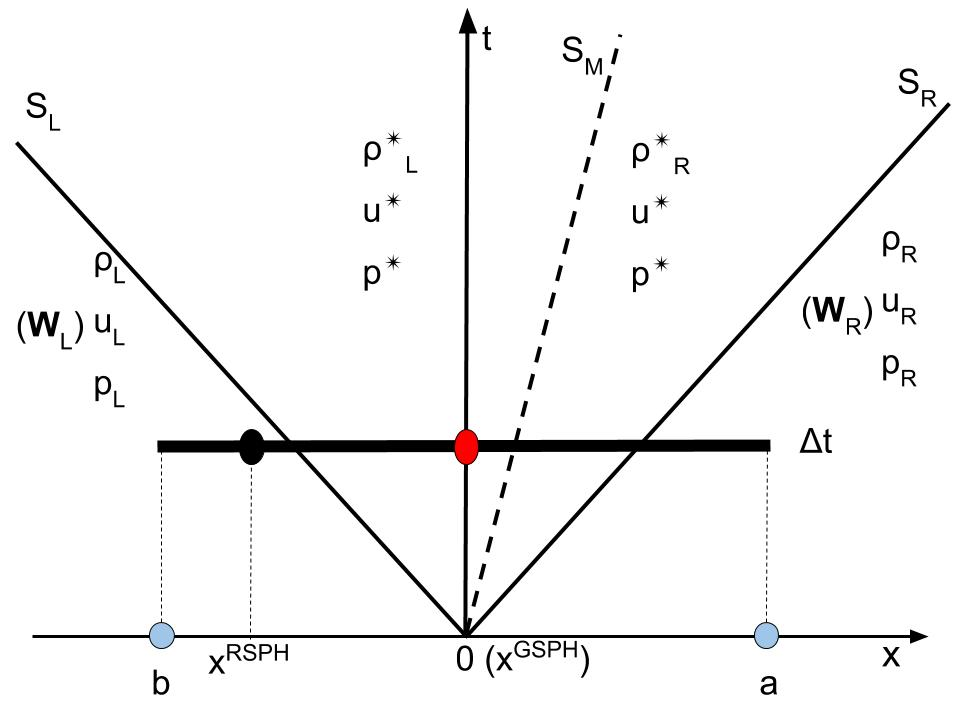
\includegraphics[width=0.5 \textwidth]{./Figures/RSPH-GSPH}
    \caption{Evaluating of the starred values in RSPH and GSPH for paired particles $a$ and $b$. The local Riemann problem is defined by state of particles $a$ and $b$ at $t=0$ according to Eq. (\ref{eq:Riemann-Prob-define-L-rho}) - Eq. (\ref{eq:Riemann-Prob-define-R-p})). The horizontal bold solid line indicate the sample range in the solution of the Riemann problem defined between particle $a$ and particle $b$ at given time $t=\Delta t$. The dark ellipse is an example sample point of RSPH with the random number $\epsilon < \frac{1}{2}$. Depending on the random number $\epsilon$, the sample points can be anywhere on the horizontal bold solid line. The white ellipse is the imaginary interface for GSPH, which is fixed. The sampled state is assigned to starred velocity and pressure in Eq. (\ref{eq:gov-gsph-v-simple-form}) and Eq. (\ref{eq:gov-gsph-e-simple-form}) for both GSPH and RSPH.}
    \label{fig:pick-up-state-GSPH-RSPH}
\end{figure}

A short comments regarding the difference between application of RCM method in SPH and its application in finite volume method. In finite volume method, for 1D case, two Riemann Problems are definied on interfaces of both sides. the superposition of solutions of these two Riemann problems is taken as local solution within the cell and the sampled single state is assigned to the cell center. In RSPH, only one Riemann problem is defined between two particles and the sampled single state (the $p^{\ast}$ and $u^{\ast}$) is used in momentum and energy updating.

$u^{\ast}$ is velocity in a 1D local space and needs to be projected back to global space to obtain $\textbf{v}^{\ast}$ in cases of multi-dimensional implementations. One of such back-project approximations is:
\begin{equation}
\textbf{v}^{\ast}_{a b}=u^{\ast}_{a b} \hat{\textbf{r}}_{a b} + \left [\frac{\textbf{v}_{a} + \textbf{v}_{b}}{2} - \frac{u_L + u_R}{2} \hat{\textbf{r}}_{a b}\right]
\label{eq:RP-project-to-3d-arithmetic}
\end{equation}
In Eq. (\ref{eq:RP-project-to-3d-arithmetic}), the arithmetic average of shear velocity is taken as the shear velocity at the sample points. Alternative approximation might be distance weighted average or Roe average (weighted by square root of density). If $q_{a b}^{\ast}$ is assumed to be zero, then distance weighted average will degenerate to the arithmetic average.
Such back projection is required for both GSPH and RSPH.

We have to mention that it is strange in GSPH to assume an imaginary interface, which never need in RSPH. And that's one of the reasons why we like RSPH more.

\subsection{Non-iterative Riemann solvers} \label{sec:RP-solver}
The starred variable $p^{\ast}$ and $u^{\ast}$ represent the interpolated pressure and velocity at certain point (an imaginary interface in GSPH or a randomly sampled poit in RSPH) along the line joining the pairs of two particles. They do not have to be obtained by solving a Riemann problem. However, $p^{\ast}$ and $u^{\ast}$ obtained by solving a Riemann problem provides necessary and sufficient dissipation needed to capture discontinuities and stabilize the scheme.

The exact Riemann solver, even though more accurate and robust, requires an iterative root finding, and hence is computational inefficient. For governing equations other than well studied ones, such as Euler equations, there is no iterative Riemann solver available. Non-iterative approximate Riemann solvers can relieve these drawbacks of exact Riemann solvers. Among the available Riemann solvers \citep{rider1994review, luo2004computation, puri2014approximate}, we adopted the HLLC approximate Riemann solver.
The HLLC solver is a 3-wave approximate Riemann solver proposed by \citet{toro1994restoration}. In this work, we adopt the formulation of the HLLC solver proposed by \citet{luo2004computation} for multi-material, underwater explosions in their ALE scheme. This Riemann solver has the properties of being positivity preserving for scalar quantities, entropy satisfying and to exact preserve isolated contacts.

Equation (\ref{eq:RP_solver_HLLC_u}) and (\ref{eq:RP_solver_HLLC_pu}) are the approximate solution to the local Riemann problem, written in term of $p$ and $pu$ as functions of local coordinate $q$.
\begin{equation}
p \left( q \right) =  \begin{cases} 
      p_L & if \  S_L \Delta t> q \\
      \frac{S_M}{S_L - S_M}\left [ (S_L - \hat{u}_L) M_L + (\hat{p}- p_L) \right] + \hat{p} & if \  S_L \Delta t \leq q \leq S_M \Delta t \\
      \frac{S_M}{S_R - S_M}\left [ (S_R - \hat{u}_R) M_R + (\hat{p}- p_R) \right] + \hat{p} & if \  S_M \Delta t \leq q \leq S_R \Delta t \\
      p_R & if \  S_R \Delta t < q
\end{cases}
\label{eq:RP_solver_HLLC_u}
\end{equation}
\begin{equation}
(pu) \left( q \right)  =  \begin{cases} 
      p_L u_L& if \  S_L \Delta t > q \\
      \frac{S_M}{S_L - S_M}\left [ (S_L - \hat{u}_L) E_L + (\hat{p} S_M - p_L \hat{u}_L) \right] + (S_M - \hat{u}_{LR}) \hat{p} & if \  S_L \Delta t \leq q \leq S_M \Delta t \\
      \frac{S_M}{S_R - S_M}\left [ (S_R - \hat{u}_R) E_R + (\hat{p} S_M- p_R \hat{u}_R) \right] + (S_M + \hat{u}_{LR}) \hat{p} & if \ S_M \Delta t \leq q \leq S_R \Delta t\\
      p_R u_R & if \  S_R \Delta t < q
\end{cases}
\label{eq:RP_solver_HLLC_pu}
\end{equation}
where $\hat{u}_{LR}$ is the interface velocity and is taken as the Roe-averaged velocity on either side of the interface \citep{cheng2007high}. The quantities of $\hat{u}_R$ and $\hat{u}_L$ are velocities relative to the interface velocity.
\begin{equation}
\hat{p}= \rho_L (\hat{u}_L - S_L) (\hat{u}_L - S_M) + p_L
\end{equation}
Formulation to approximate the signal speeds $S_M$, $S_L$ and $S_R$ is given by Eq. (\ref{eq:RP-solver-HLLC-SM}) to (\ref{eq:RP-solver-HLLC-SR}).
\begin{eqnarray}
S_M= \frac{\rho_R \hat{u}_R (S_R - \hat{u}_R) - \rho_L \hat{u}_L (S_L - \hat{u}_L) + p_L - p_R}{\rho_R (S_R - \hat{u}_R) - \rho_L (S_L - \hat{u}_L)} \label{eq:RP-solver-HLLC-SM} \\
S_L = min (\hat{u}_L - c_L, -c_{LR}) \label{eq:RP-solver-HLLC-SL} \\
S_R = max (\hat{u}_R - c_R, c_{LR}) \label{eq:RP-solver-HLLC-SR}
\end{eqnarray}
where $c_{LR}$ is the relevant Roe averaged sound speed \citep{cheng2007high}. 

Besides HLLC, another 2-wave approximate Riemann solver, the Roe Riemann solver \citep{roe1981approximate}, is also adopted in GSPH.
Roe Riemann solver is proposed by \citet{roe1981approximate} to linearize the Euler equations and approxiamte the solution of non-linear system by a system of linear equations. The characteristic decomposition of the linearized Lagrangian flux and Jacobia matrices are used to write the flux. \citet{rider1994review} proposed an algebraic averaging of the Lagrangian variables, which is adopted in this work. Since Roe solver is only used in GSPH. We directly provide here the resulting starred values of the pressure and velocity \citep{puri2014approximate}: 
\begin{eqnarray}
u^{\ast} = \frac{1}{2} \left[ u_L + u_R - \frac{1}{C_{LR}} (p_R - p_L) \right] \label{eq:RP-solver-ROE-u} \\
p^{\ast} = \frac{1}{2}\left[ p_L + p_R - C_{LR} (u_R - u_L) \right] \label{eq:RP-solver-ROE-p}
\end{eqnarray}
Where $C_{LR}$ is the averaged Lagarangian sound speed at the interface.
\begin{equation}
C_{LR} = \sqrt{\gamma p_{LR} \rho_{LR}}
\end{equation}

\subsection{Binary Van Der Corput pseudo-random numbers} \label{sec:Van-Der-Corput-random-num}
The random number $\epsilon$ is used to determine the sample location $q_{ab}^{RSPH}$. The quantity of the computed RCM solution depends crucially on the random number $\{\epsilon ^n\}$. We adopt the Van Der Corupt pseudo-random number sequence \citep{hammersley2013monte} in this investigation following \citet{colella1982glimm}.

A general Van Der Corupt pseudo-random number sequence depends on two parameters $x_1$ and $x_2$ with $x_1 > x_2 > 0$, both are integer and relatively prime. The sequence is formally defined as \citep{hammersley2013monte}:
\begin{equation}
\epsilon ^n = \sum_{i=0}^{s} H_i x_1^{-(i+1)}
\label{eq:Van-Der-Corput-pseudo-random-num}
\end{equation}
where
\begin{equation}
H_i = x_2 a_i(mod \ x_1)
\label{eq:Van-Der-Corput-pseudo-random-num-Hi}
\end{equation} 
\begin{equation}
n = \sum_{i=0}^{s} a_i x_1^i
\label{eq:Van-Der-Corput-pseudo-random-num-n}
\end{equation} 
Equation (\ref{eq:Van-Der-Corput-pseudo-random-num-n}) gives the binary expansion of n when we take $x_1$ as $2$. For example,
\begin{equation}
5=1 \times 2^0 + 0 \times 2^1 + 1 \times 2^2
\end{equation}
with $m=2$. 

The next stage is to find the coefficient $H_i$ according to Eq. (\ref{eq:Van-Der-Corput-pseudo-random-num-Hi}). If we take $x_2 = 1$, for which case, $H_i = a_i, \ \forall i$. Having $H_i$, $x_1$ and $s$ ready, the random number $\epsilon ^n $ can be easily obtained according to Eq. (\ref{eq:Van-Der-Corput-pseudo-random-num}).
We take $x_1=2$  and $x_2 =1$ in this paper. Other combinations of $x_1$ and $x_2$ were also discussed by \citet{toro2013riemann}. A desirable statistical property of the sequence $\{\epsilon ^n\}$ is that $\{\epsilon ^n\}$ be uniformly distributed over $[0,1]$.
 
The arithmetic mean and the standard deviation of 200 binary Van Der Corput pseudo-random numbers are $0.49459$ and $0.28885$. The chi-square statistic (see \citet{toro2013riemann} for its calculation) $\chi_{sq}$ is $1.0000$. 
The binary Van Der Corput pseudo-random numbers are generated offline to save computational time.

%\subsection{Convergence}

\subsection{RSPH algorithm (the PESB algorithm)}
The Godunov's method is summarized as a REA (reconstruct, evolve, average) algorithm. Here we summarize the RSPH algorithm as a PESB (project, evolve, sample, back-project) algorithm. 
\begin{itemize}
\item For any two pair of particles, establish a local coordinate system whose axis joints these two particles then project the primitive variables vector onto the local coordinate system.
\item Evolve the hyperbolic equation exactly or approximately with Riemann problem defined by the projected data to obtain a solution between these two particles.
\item Sample these solutions between the particles pair to pick up a state and assign it to $p^{\ast}$ and $u^{\ast}$
\item Project $p^{\ast}$ and $u^{\ast}$ from local coordinate system back to the global coordinate system obtaining $p^{\ast}$ and $\textbf{v}^{\ast}$.
\end{itemize}
PESB algorithm is integrated into framework of SPH discretization to update physical quantities in time. PESB also fit well with GSPH, for which, the sample step is not stochastic randomly sample.

\section{Numerical tests}
We carry out several numerical tests using SPH, RSPH and GSPH in this section.
1D shock tube tests are conducted to compare standard SPH, GSPH and RSPH. Comprehensive shock tube tests are also conducted to check the capacity of RSPH for different situations. In addition, order of accuracy is investigated based on 1D shock tube problem. 
In the last subsection, a 3D free jet flow is simulated with SPH, GSPH and RSPH to check equivalent overall dissipation introduced by each method.

Input parameters for 1D tests can be found in Table \ref{tab:1D-shock-input_parameters}. 
\begin{table}[htp]
\centering
      \caption{Overview of 1D shock tube tests}		
	  \begin{tabular}{lrrrrrrrrrr}
	    \hline
	          & $\rho_L$ & $p_L$ &$v_L$ & $\rho_R$ & $p_R$ &$v_R$ & $m$ & $[x_L, x_R]$ & $t_f$\\
	    \hline
	    Test 1 & $1.0$ & $1.0$ &$0$ & $0.25$ & $0.1795$ &$0$ & $0.003$  & $[-0.4, 0.4]$ & $0.17$\\
	    	Test 2 & $1.0$ & $1.0$ &$0$ & $0.5$ & $0.2$ &$0$ & $0.003$  & $[-0.4, 0.4]$ & $0.2$\\
	    	Test 3 & $2.0$ & $1.95$ &$1.0$ & $1.0$ & $1.95$ &$-1.0$  & $0.006$  & $[-0.4, 0.4]$ & $0.13$\\
	    Test 4 & $1.0$ & $2.4$ &$8.0$ & $0.5$ & $0.4$ &$-0.25$ & $0.003$  & $[-0.4, 0.4]$ & $0.05$\\
	    	Test 5 & $1.0$ & $-2.0$ &$0.4$ & $1.0$ & $0.4$ &$2.0$ & $0.003$  & $[-0.4, 0.4]$ & $0.18$\\
	    	Test 6 & $1.0$ & $0$ &$1000$ & $1.0$ & $0$ &$0.01$ & $0.003$  & $[-0.5, 0.5]$  & $0.01$\\
	    \hline
	  \end{tabular}
	  \label{tab:1D-shock-input_parameters}
\end{table}
where, subscript $L$ refers left side and $R$ for right side. $m$ is particle mass, initial interval between adjacent particles are adjusted to guarantee equal particle mass. $t_f$ is the time to terminate simulation and plotting the results. Equal particle mass is assigned to all particles. The $x$ axis in all plots is normalized by time, that is $x/t_f$, in plots for shock tube tests results.

Test 1 consists of a left rarefaction, a right travelling contact and a right shock. Density increases at down wind of contact wave.
Test 2 also consists of a left rarefaction, a right travelling contact and a right shock. Density decreases at down wind of contact wave.
Test 3 includes double expansion waves. The initial density are different at right and left hand side.
Test 4 is a double shock tests with different initial density on the right side and left side.
Test 5 and Test 6 are two extreme cases. Test 5 is a cavity flow while test 6 is a strong blast flow.

\subsection{Comparison of RSPH with standard SPH and GSPH}
\begin{figure}[htp]
    \centering
    \begin{minipage}{.495\textwidth}
        \centering
        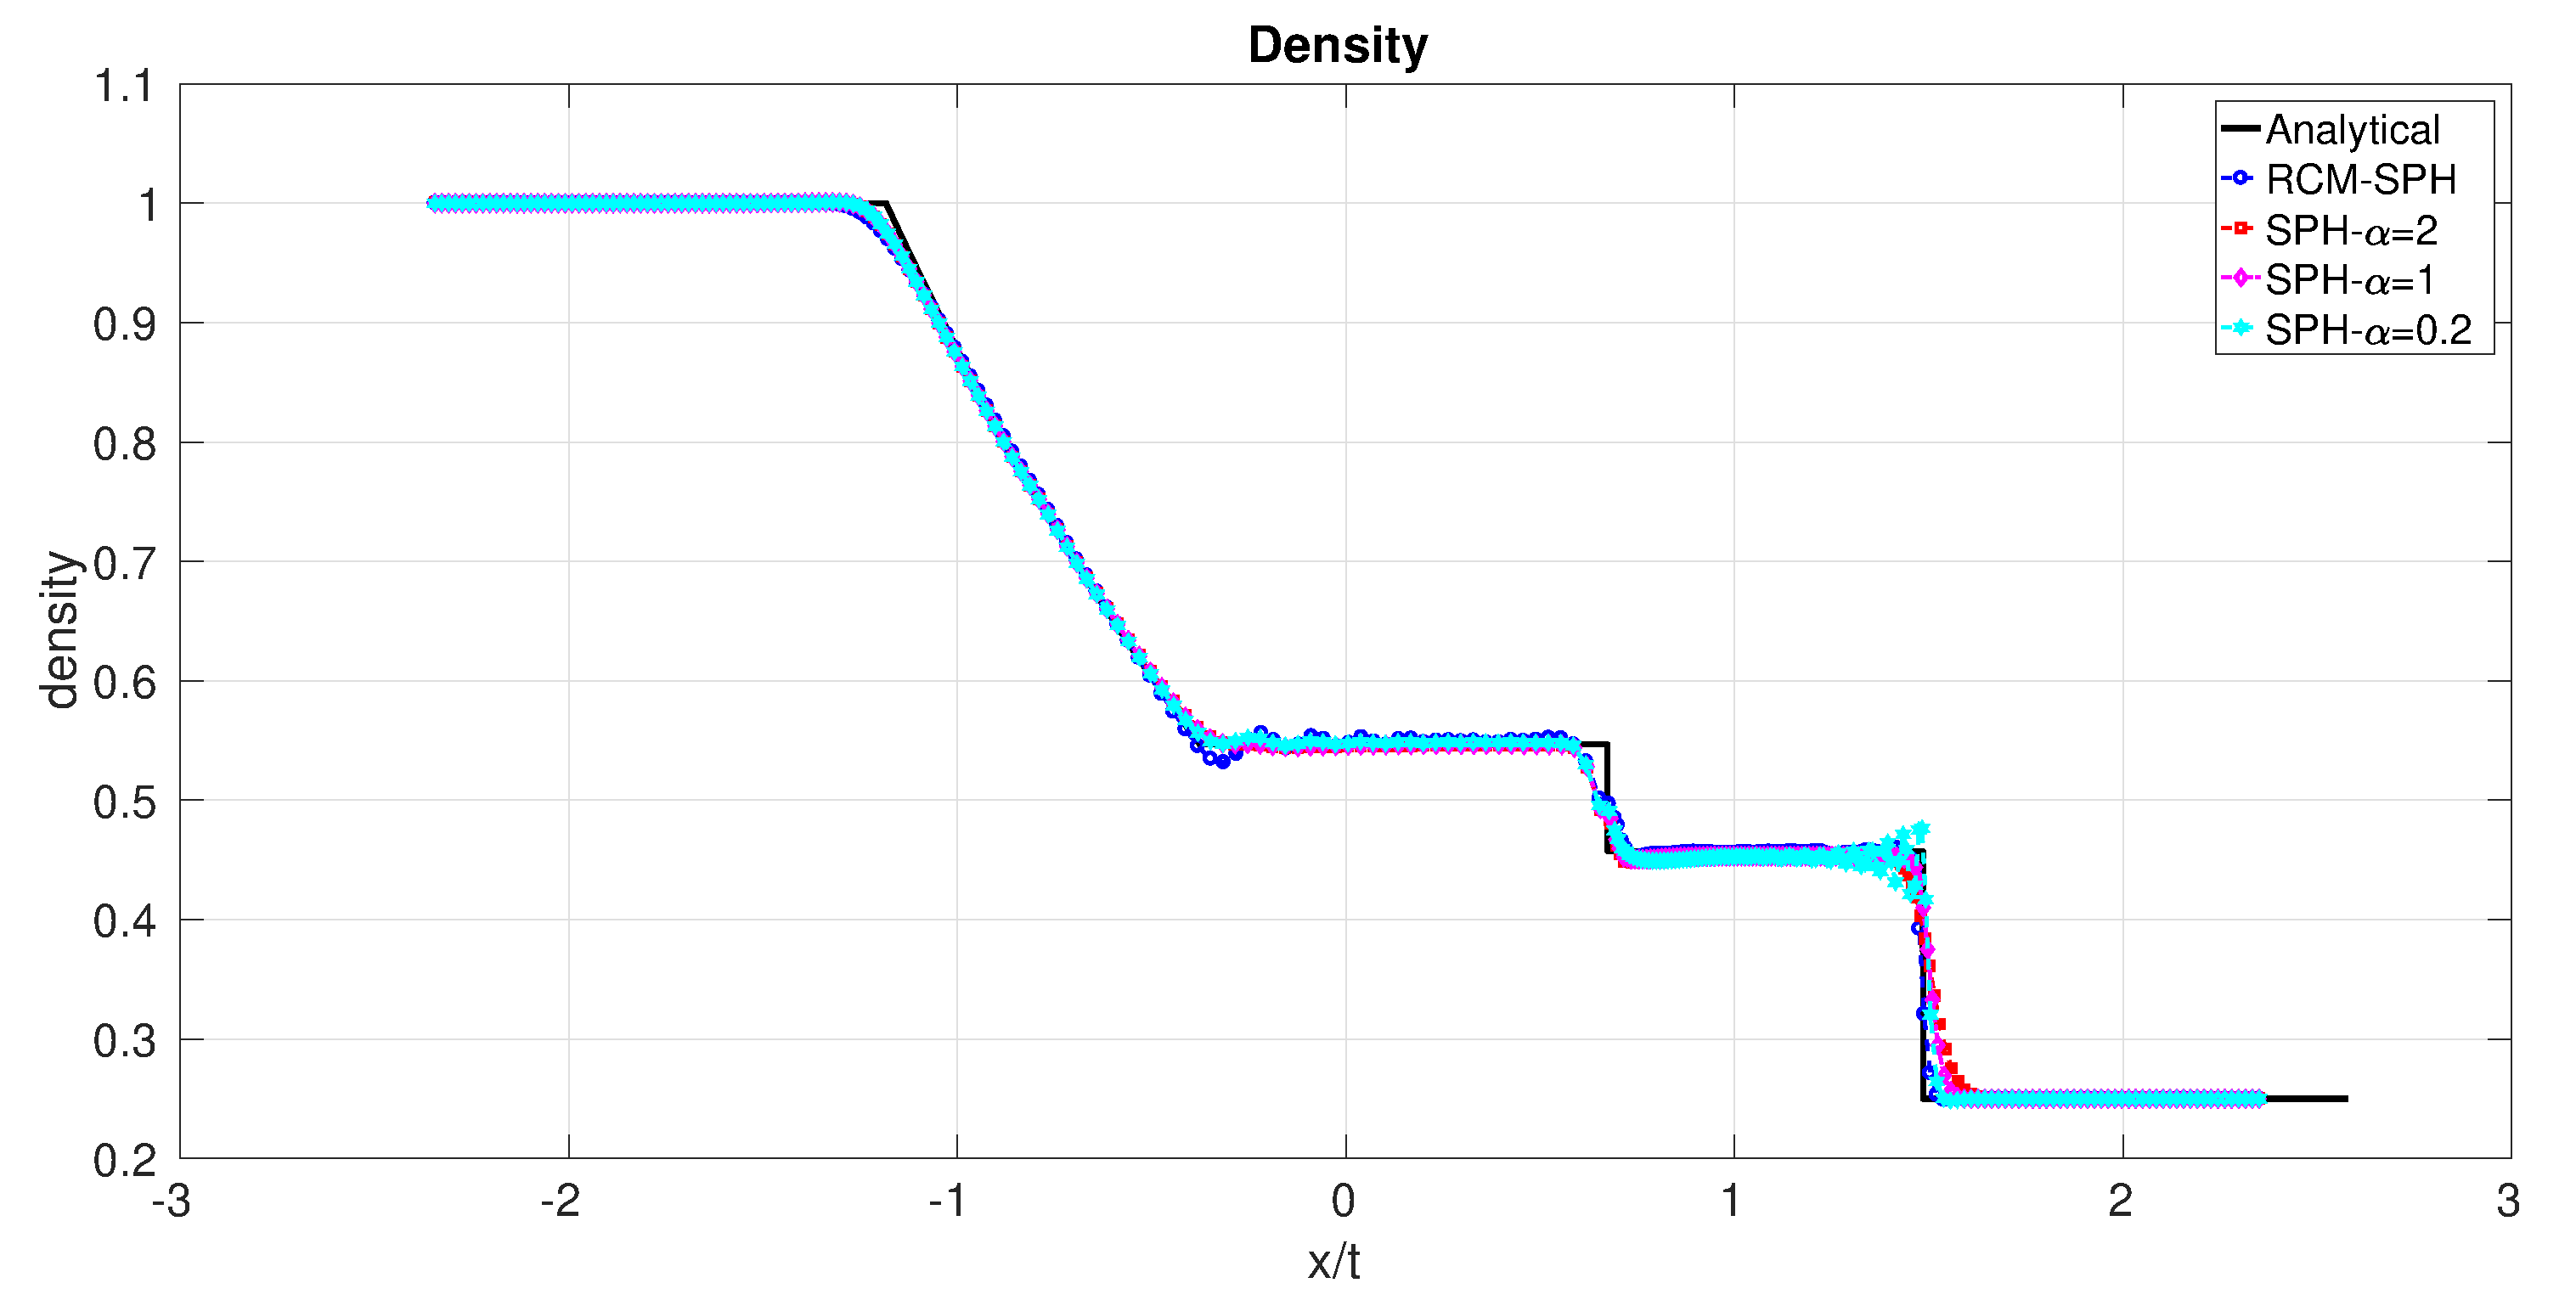
\includegraphics[width=0.99 \textwidth]{./Figures/Sod/RCM-Sod-SPH-alf-rho}
    \end{minipage}%
    \begin{minipage}{.495 \textwidth}
        \centering
        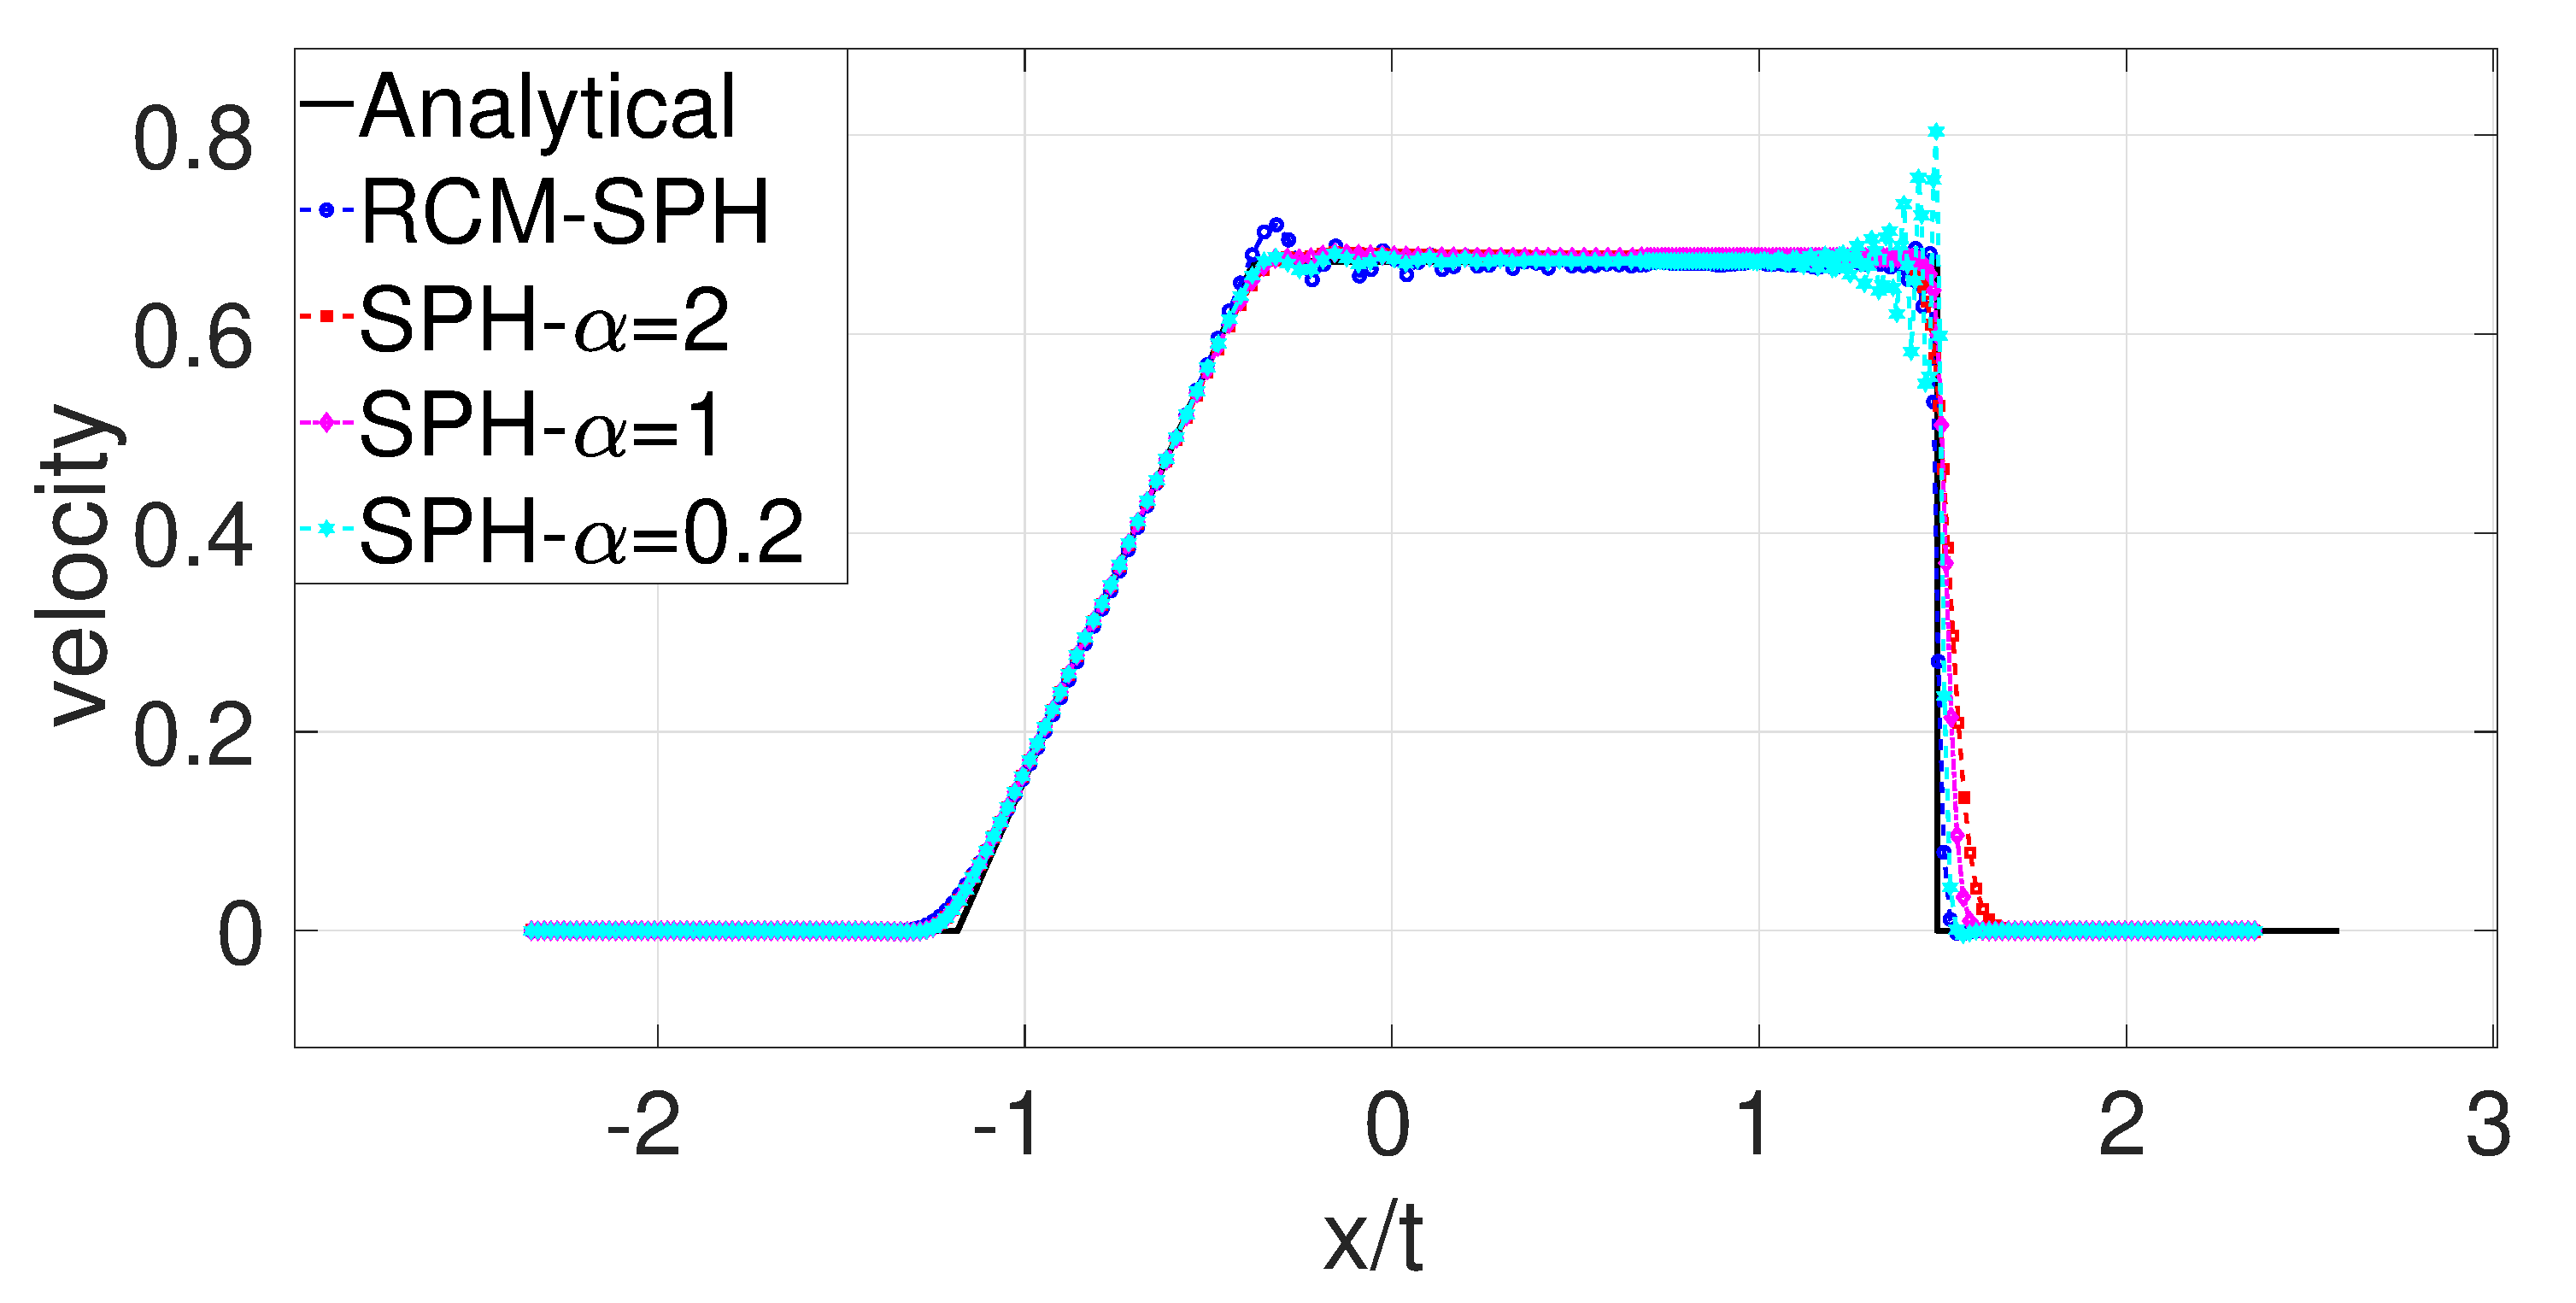
\includegraphics[width=0.99 \textwidth]{./Figures/Sod/RCM-Sod-SPH-alf-v}
    \end{minipage}%
    \\
    \begin{minipage}{.495\textwidth}
        \centering
        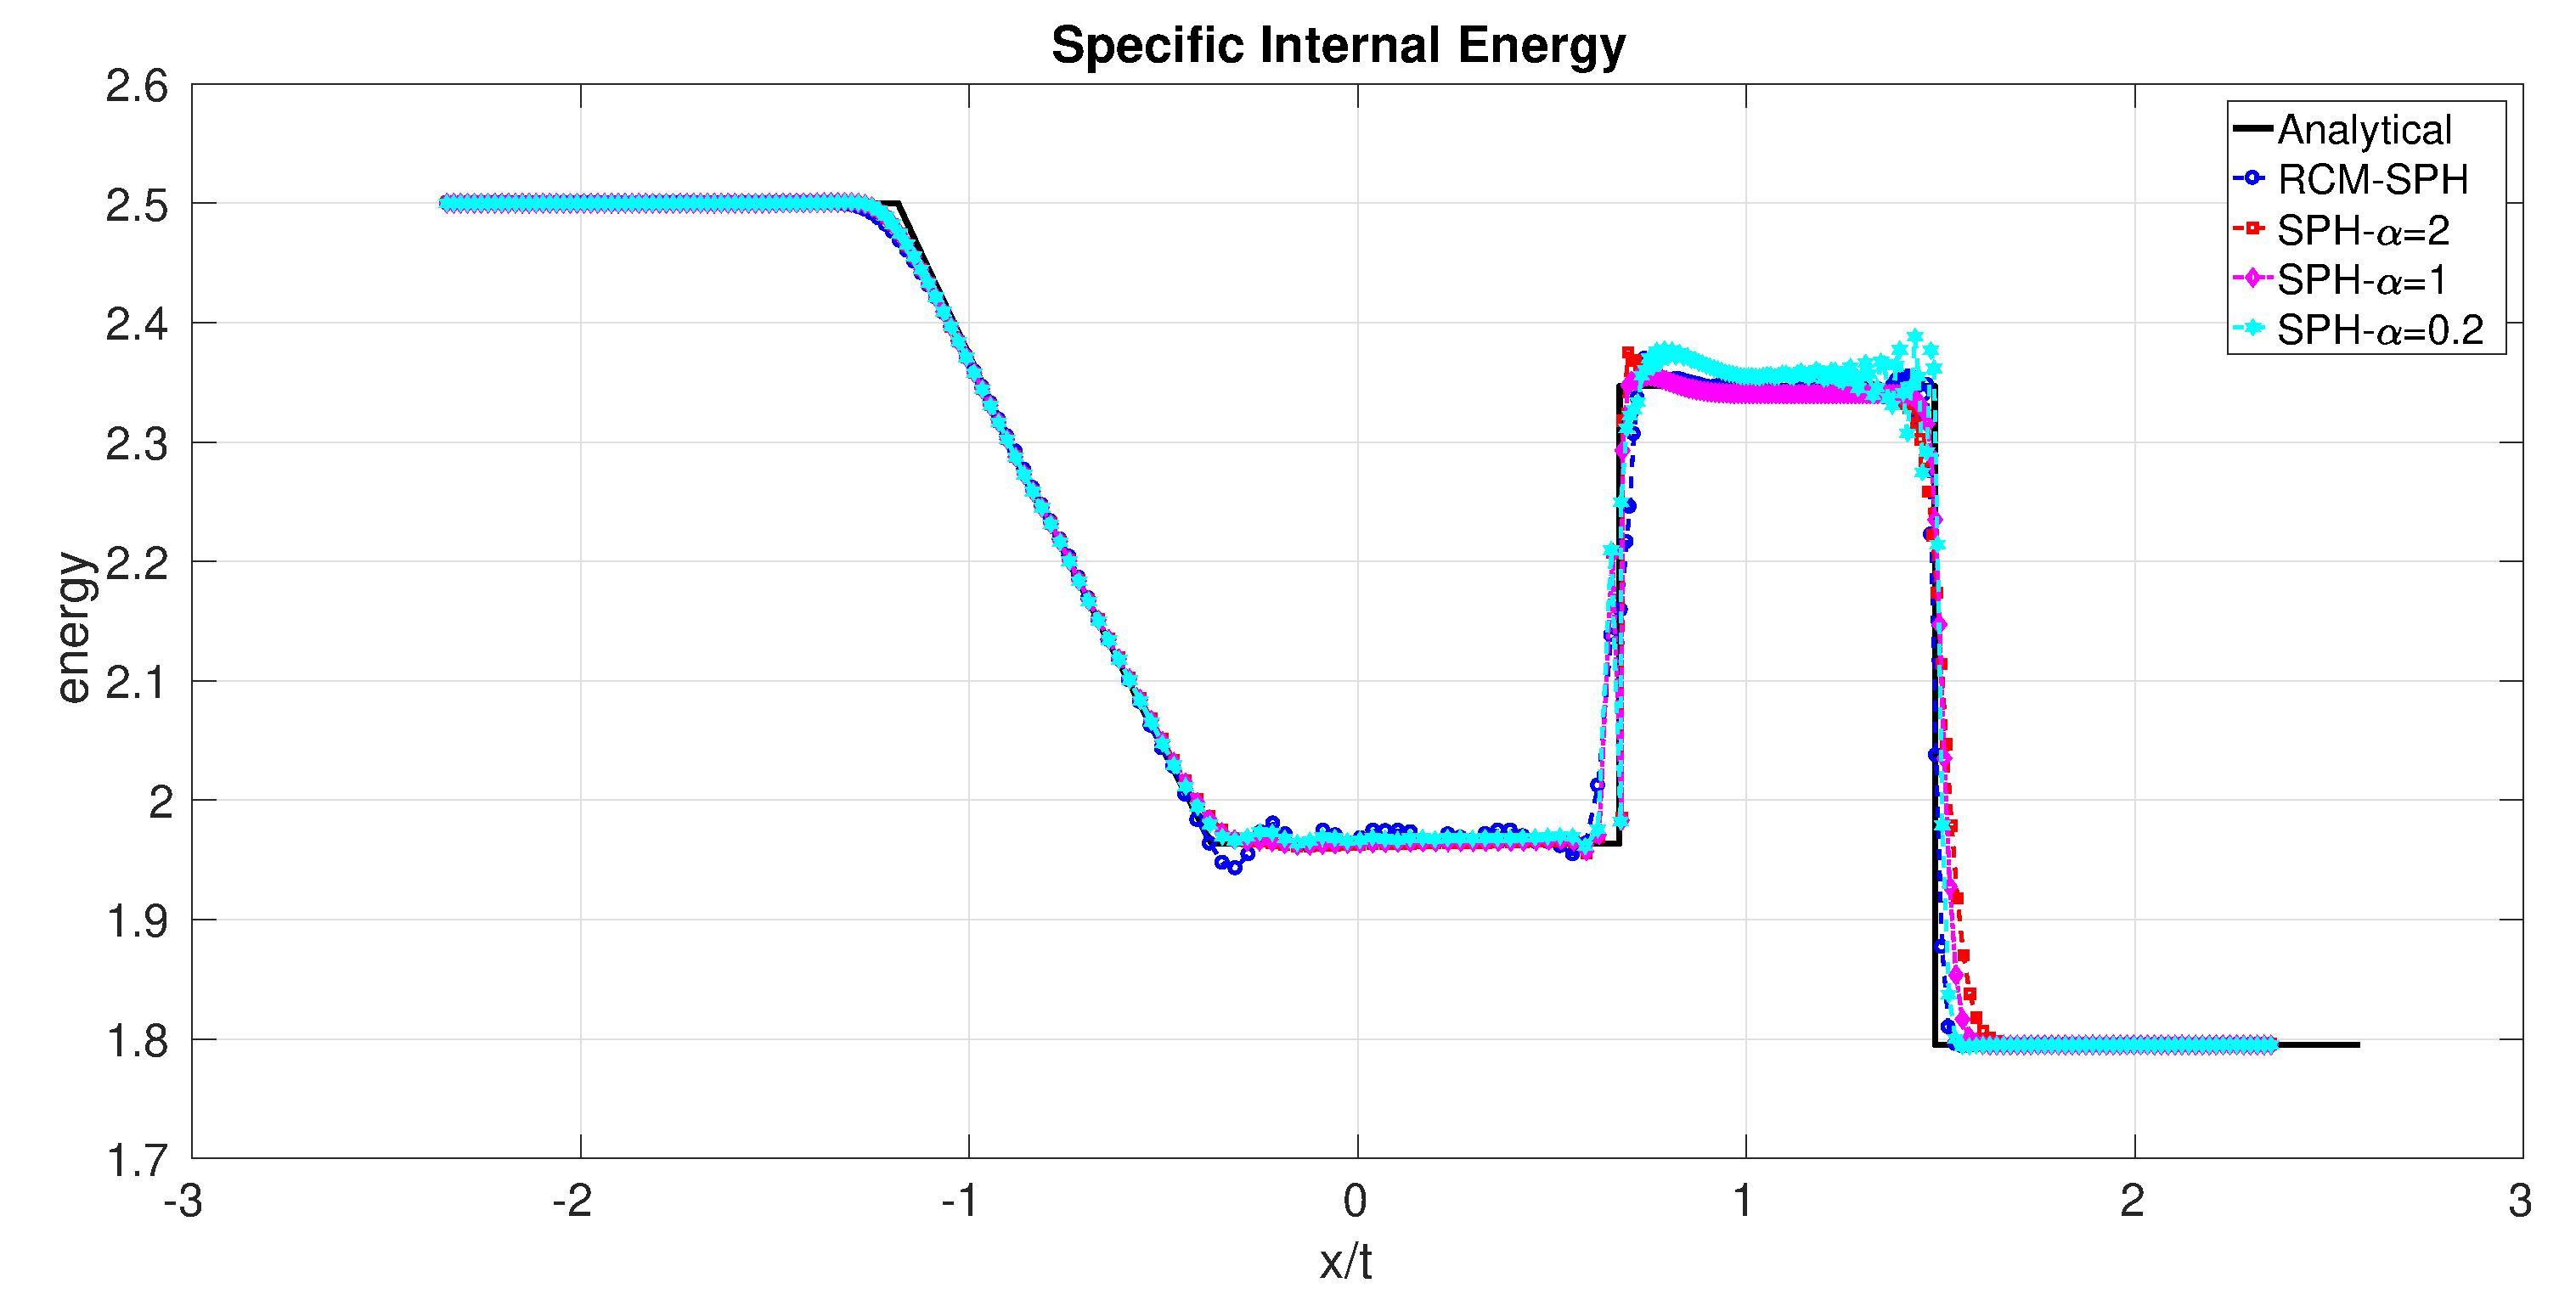
\includegraphics[width=0.99 \textwidth]{./Figures/Sod/RCM-Sod-SPH-alf-e}
    \end{minipage}%
    \begin{minipage}{.495 \textwidth}
        \centering
        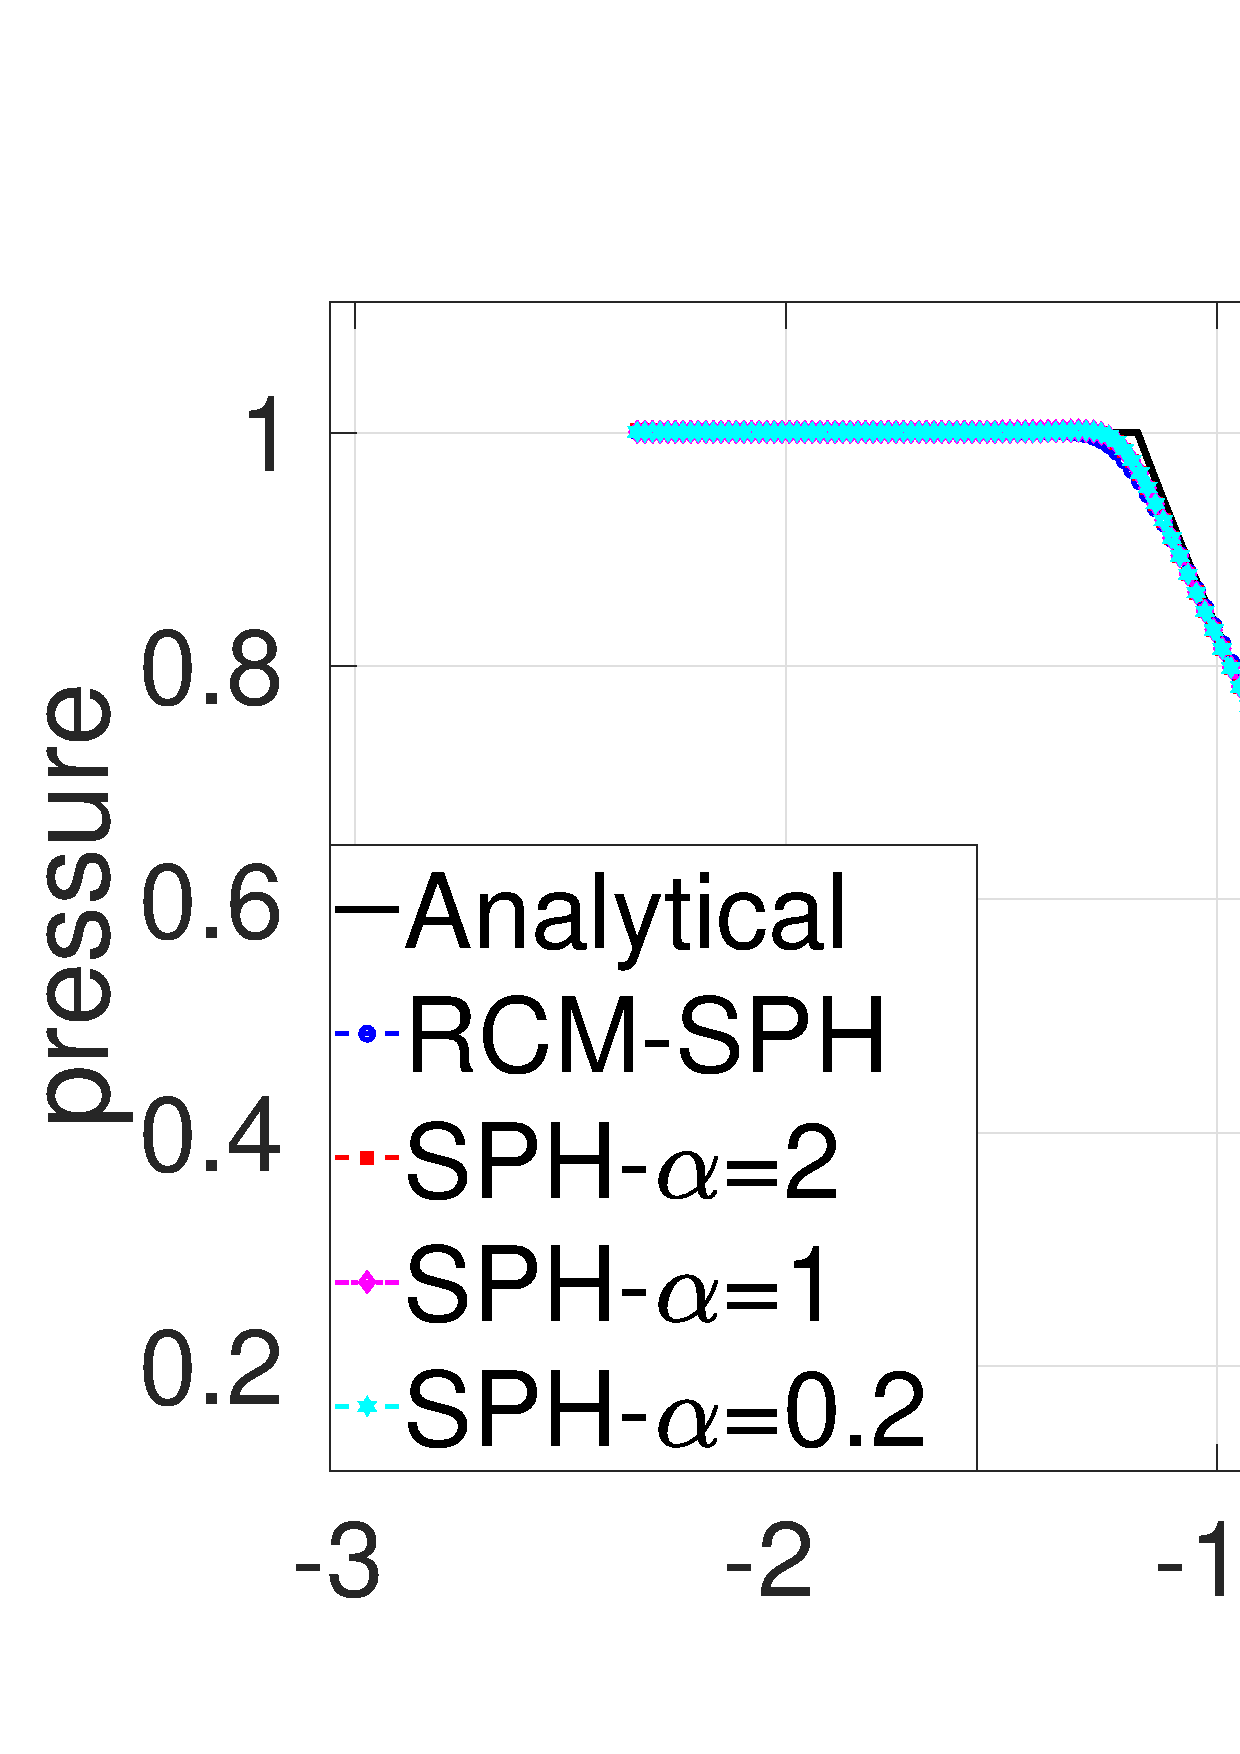
\includegraphics[width=0.99 \textwidth]{./Figures/Sod/RCM-Sod-SPH-alf-p}
    \end{minipage}% 
    \\
    \begin{minipage}{.495\textwidth}
        \centering
        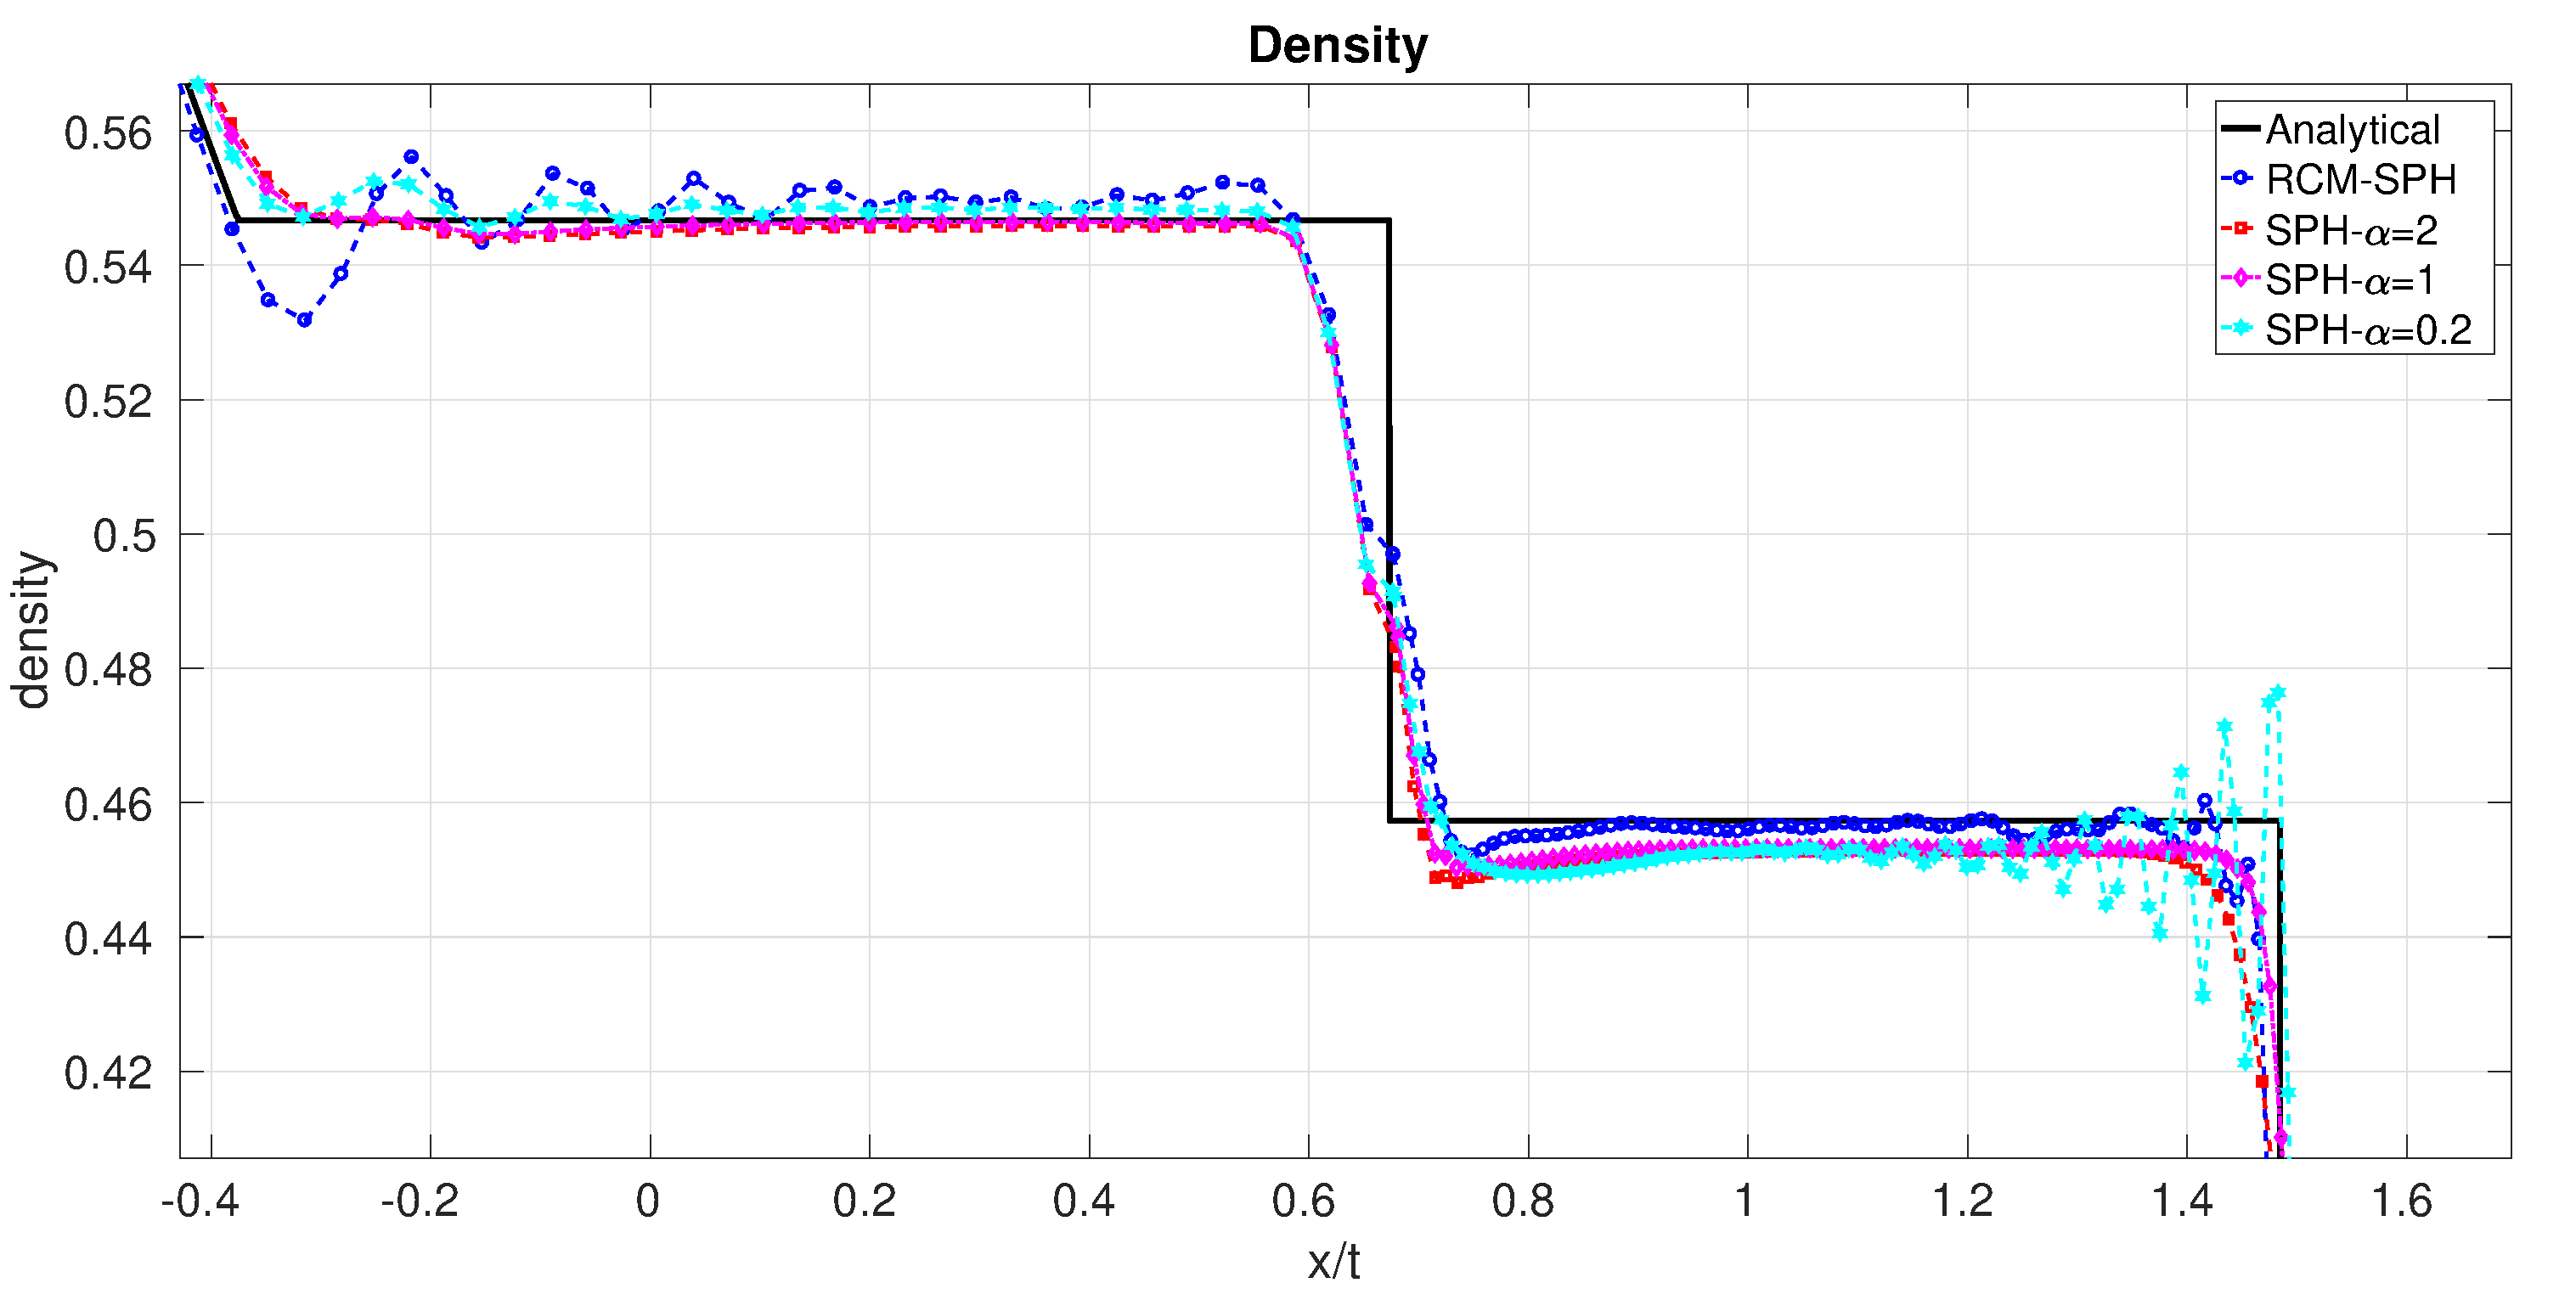
\includegraphics[width=0.99 \textwidth]{./Figures/Sod/RCM-Sod-SPH-alf-rho-zoom}
    \end{minipage}%
    \begin{minipage}{.495 \textwidth}
        \centering
        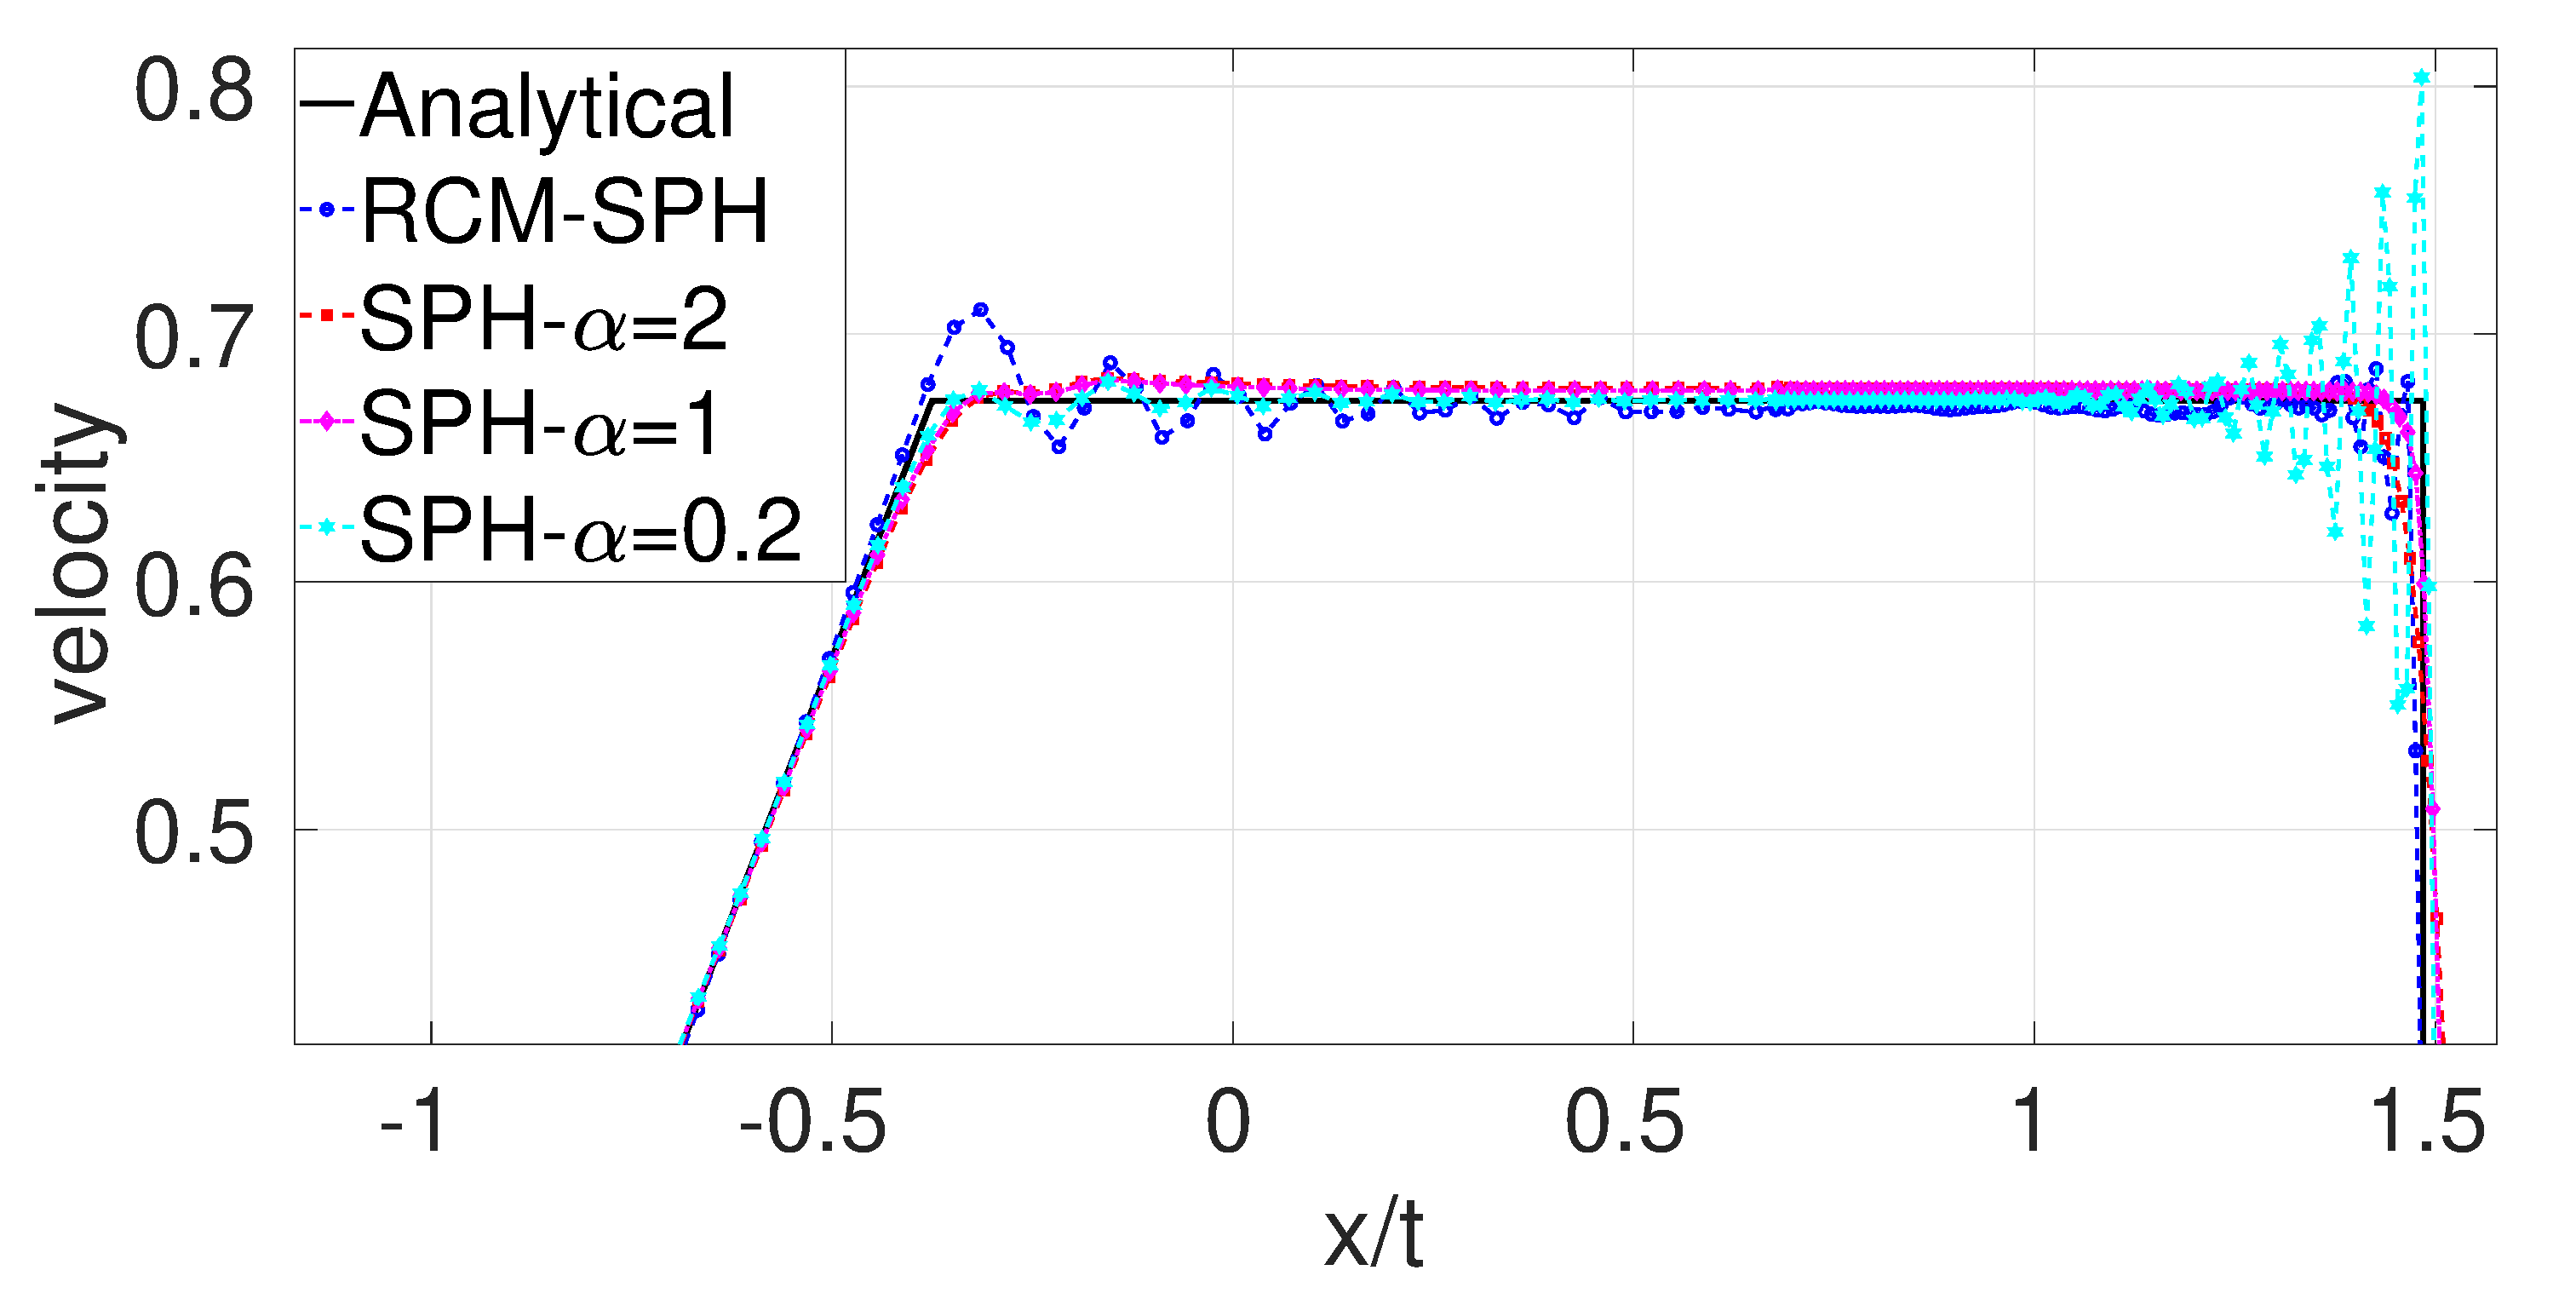
\includegraphics[width=0.99 \textwidth]{./Figures/Sod/RCM-Sod-SPH-alf-v-zoom}
    \end{minipage}% 
    \\
    \begin{minipage}{.495 \textwidth}
        \centering
        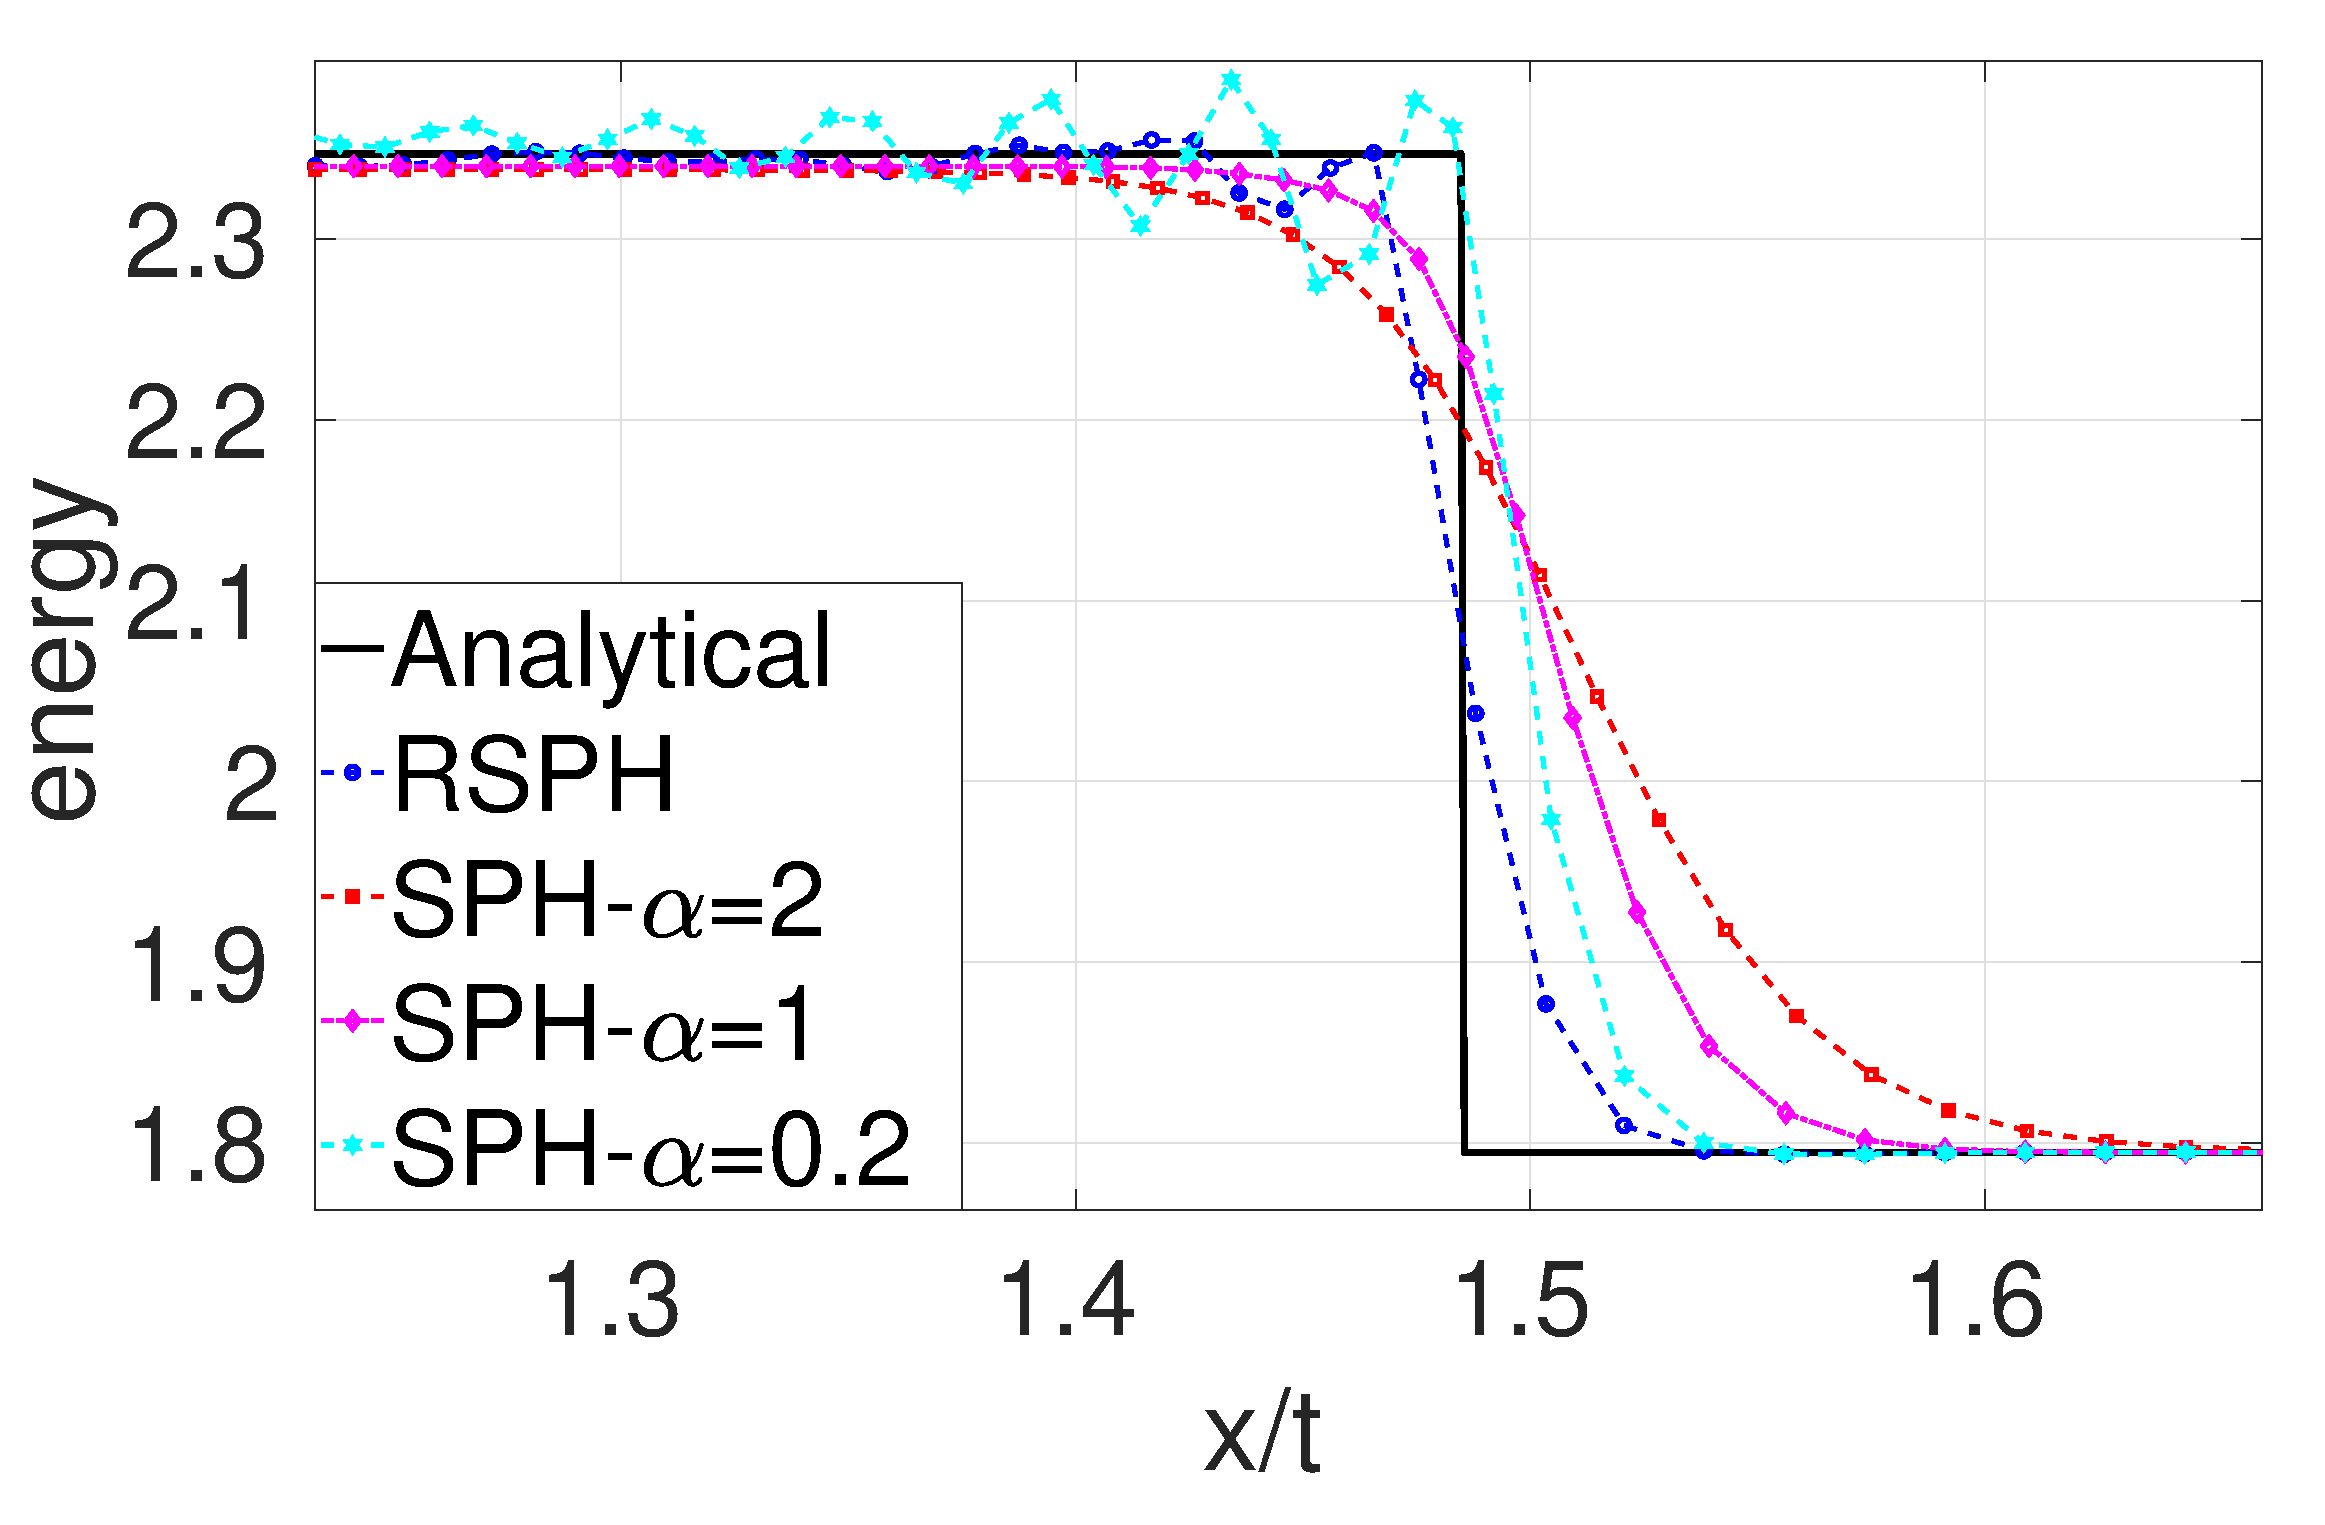
\includegraphics[width=0.99 \textwidth]{./Figures/Sod/RCM-Sod-SPH-alf-e-zoom}
    \end{minipage}% 
    \begin{minipage}{.495\textwidth}
        \centering
        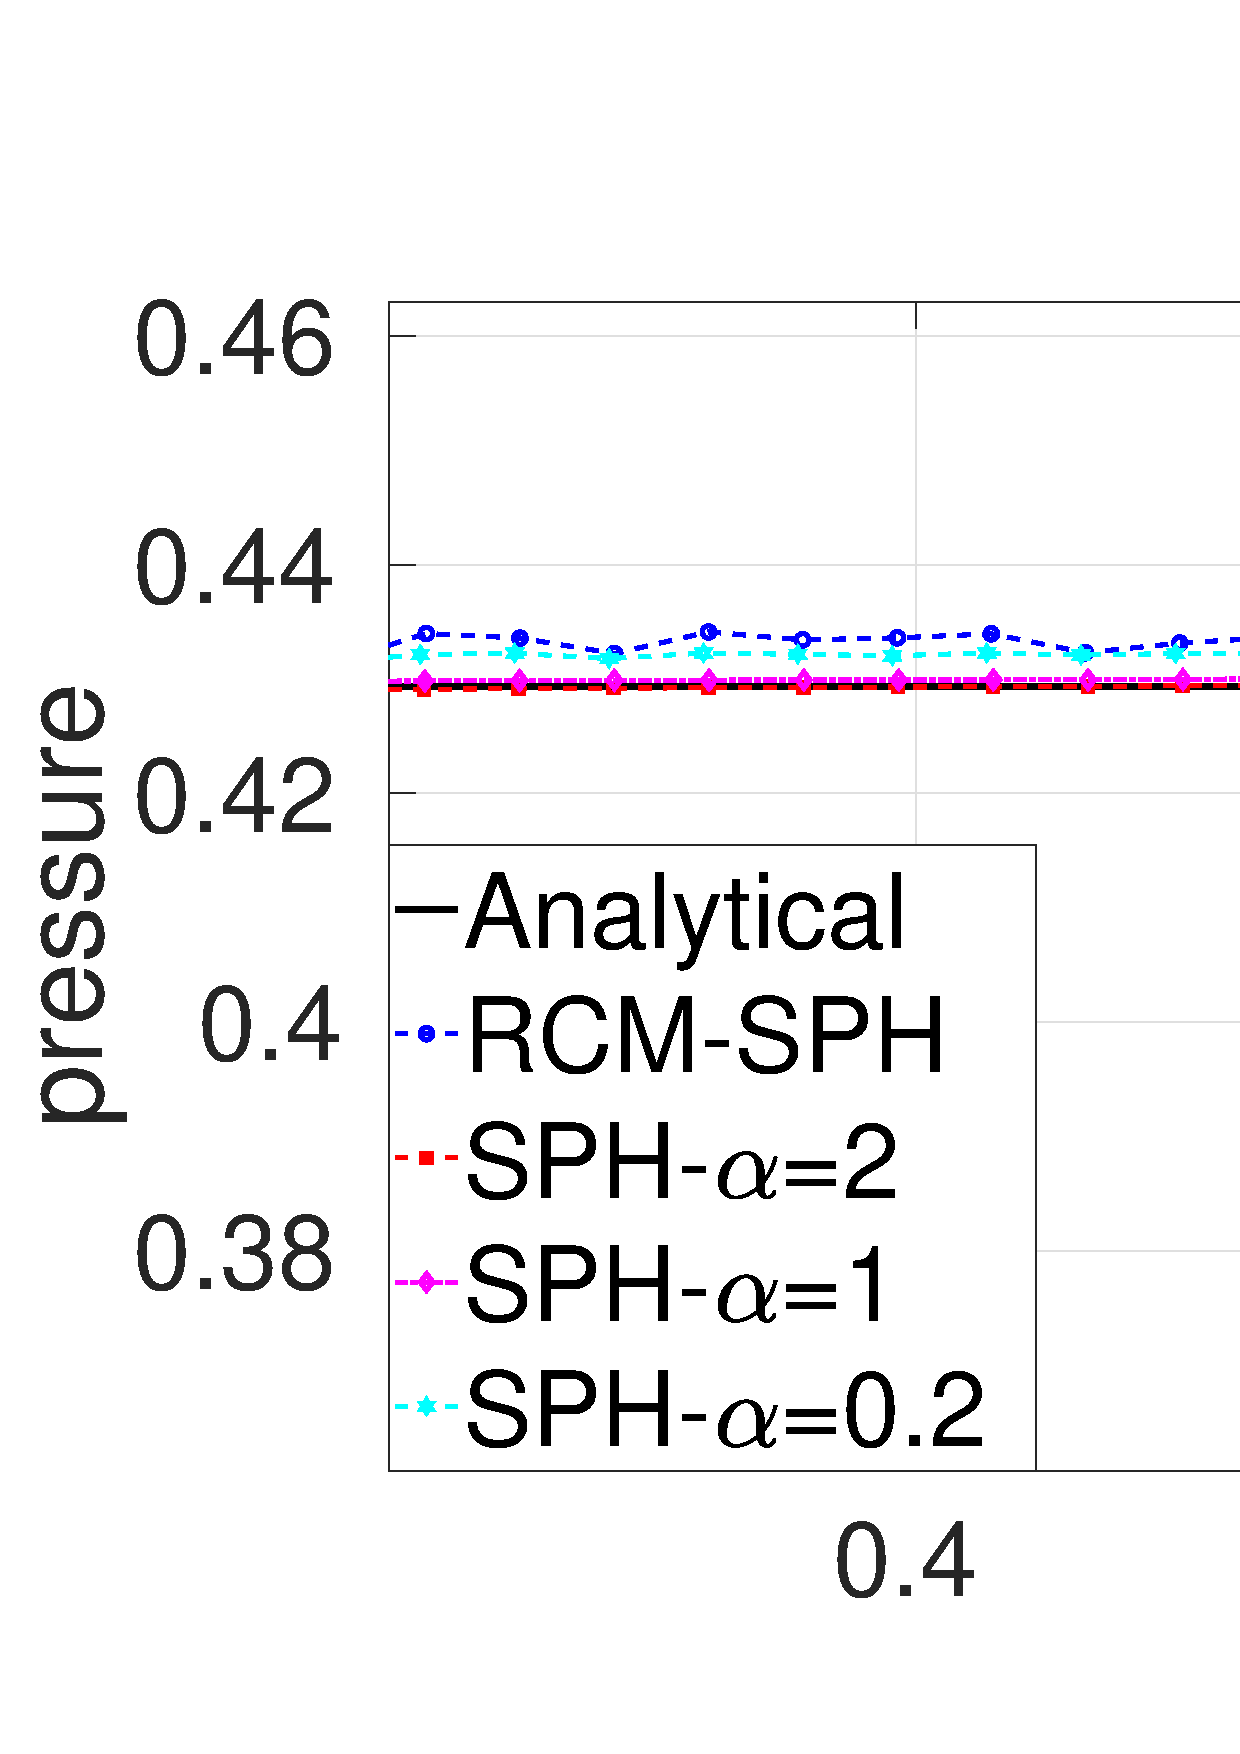
\includegraphics[width=0.99 \textwidth]{./Figures/Sod/RCM-Sod-SPH-alf-p-zoom}
    \end{minipage}%    
    \caption{Simulation results by RSPH and SPH with different artificial viscosity coefficients. The effect of artificial viscosity is illustrated through comparison. Artificial viscosity coefficients are chosen to always satisfy: $\beta=2\alpha$ in all SPH tests. The last four figures are zoomed views. Almost no fluctuation is observed when $\alpha=1$ and $\alpha=2$, illustrating that numerical fluctuation is completely suppressed if artificial viscosity is large enough. For density distribution obtained by RSPH, the fluctuations are more obvious in the area away from shock than those calculated by SPH with $\alpha=0.2$, implying that RSPH introduces smaller artificial viscosity than SPH with $\alpha=0.2$ in the area far away from shock. However, fluctuations around shock is much more obvious for SPH with $\alpha=0.2$ than RSPH, implying that RSPH introduces larger artificial viscosity than ``$\alpha=0.2$" around shock. To summarize, the equivalent artificial viscosity in RSPH is adaptive. Similar conclusion can be drew from zoomed view of velocity. The third zoomed view shows different degrees of smearing at the shock. The larger the artificial viscosity, the less sharp the solution at the shock. Since ``$\alpha=0.2$" is sharper than ``RSPH" at the shock, ``$\alpha=0.2$" introduces less dissipation at the shock, which is consistent with information implied by zoomed view of density and velocity. SPH with $\alpha=1.0$ and $\alpha=2.0$ introduces more dissipation than ``RSPH" in the area around the shock. The last zoomed view shows pressure around the contact discontinuity. It shows that RSPH get rid of pressure ``wiggle" around the contact discontinuity.}
    \label{fig:RCM-Sod-SPH-alf}
\end{figure}

Test 1 is simulated using standard SPH with different artificial viscosity coefficients, GSPH and RSPH. The comparison between RSPH and SPH using different artificial viscosity coefficients is shown in Fig. \ref{fig:RCM-Sod-SPH-alf}. In all simulations, the artificial viscosity $\beta$ is set to be twice of $\alpha$. For example, for the test ``$SPH-\alpha=2$", $\beta=4$. Several interesting observation are made based on the comparison between SPH and RSPH.
First of all, dissipation (introduced by artificial viscosity in these tests) can decays the numerical fluctuations. Numerical fluctuations are suppressed completely when large enough dissipation is introduced, for example, by using sufficiently large artificial viscosity coefficients.
%The mechanism for SPH to reduce (or completely get rid of) fluctuations should be completely different from that of new adaptive method of smoothing length. 
%The new adaptive method, reduces the sources of such fluctuations.
Secondly, the equivalent artificial viscosity coefficients introduced by RSPH varies adaptively.
As shown in Fig. \ref{fig:RCM-Sod-SPH-alf}, RSPH assigns smaller artificial viscosity coefficients (equivalent $\alpha$ much less then 0.2) at the area far away from shock and sufficient large artificial viscosity coefficients (equivalent $\alpha$ is about 1.0) around the shock. So RSPH is actually more adaptive than SPH. This feature is very desirable not only because it could eliminate parameterization and hence user intervention associated with artificial viscosity coefficients but also because it avoids introducing excessive artificial viscosity when unnecessary.
Thirdly, RSPH introduces less smearing of the shock discontinuity compared with SPH using most commonly adopted artificial viscosity coefficients ($\alpha=1.0$, $\beta=2.0$). Recall that RCM is able to resolve discontinuities as true discontinuity. RSPH, even though still smears the discontinuity in some degree, introduces much less smearing.
The last but not the least, the pressure ``wiggle" around contact discontinuity is completely eliminated by RSPH. It has been shown that thermal conduction is essential to mitigate the spurious pressure ``wiggle" at contact discontinuity in SPH \citep{monaghan1997sph, sigalotti2006shock, price2008modelling, price2012smoothed}. As for GSPH, it is reported that an implicit thermal conduction is introduced by Godunov's scheme and help suppress the anomaly \citep{puri2014approximate}. Even though, the ``wiggle" still visible in pressure distribution and velocity distribution of GSPH simulation results (for example, see figures in \citep{puri2014comparison}) and RSPH simulation results of other tests (see section \ref{sec:comprehensive-1d-tests}). ``Wiggle" in test 1, however, is completely eliminated by both GSPH and RSPH.

\begin{figure}[htp]
    \centering
    \begin{minipage}{.495\textwidth}
        \centering
        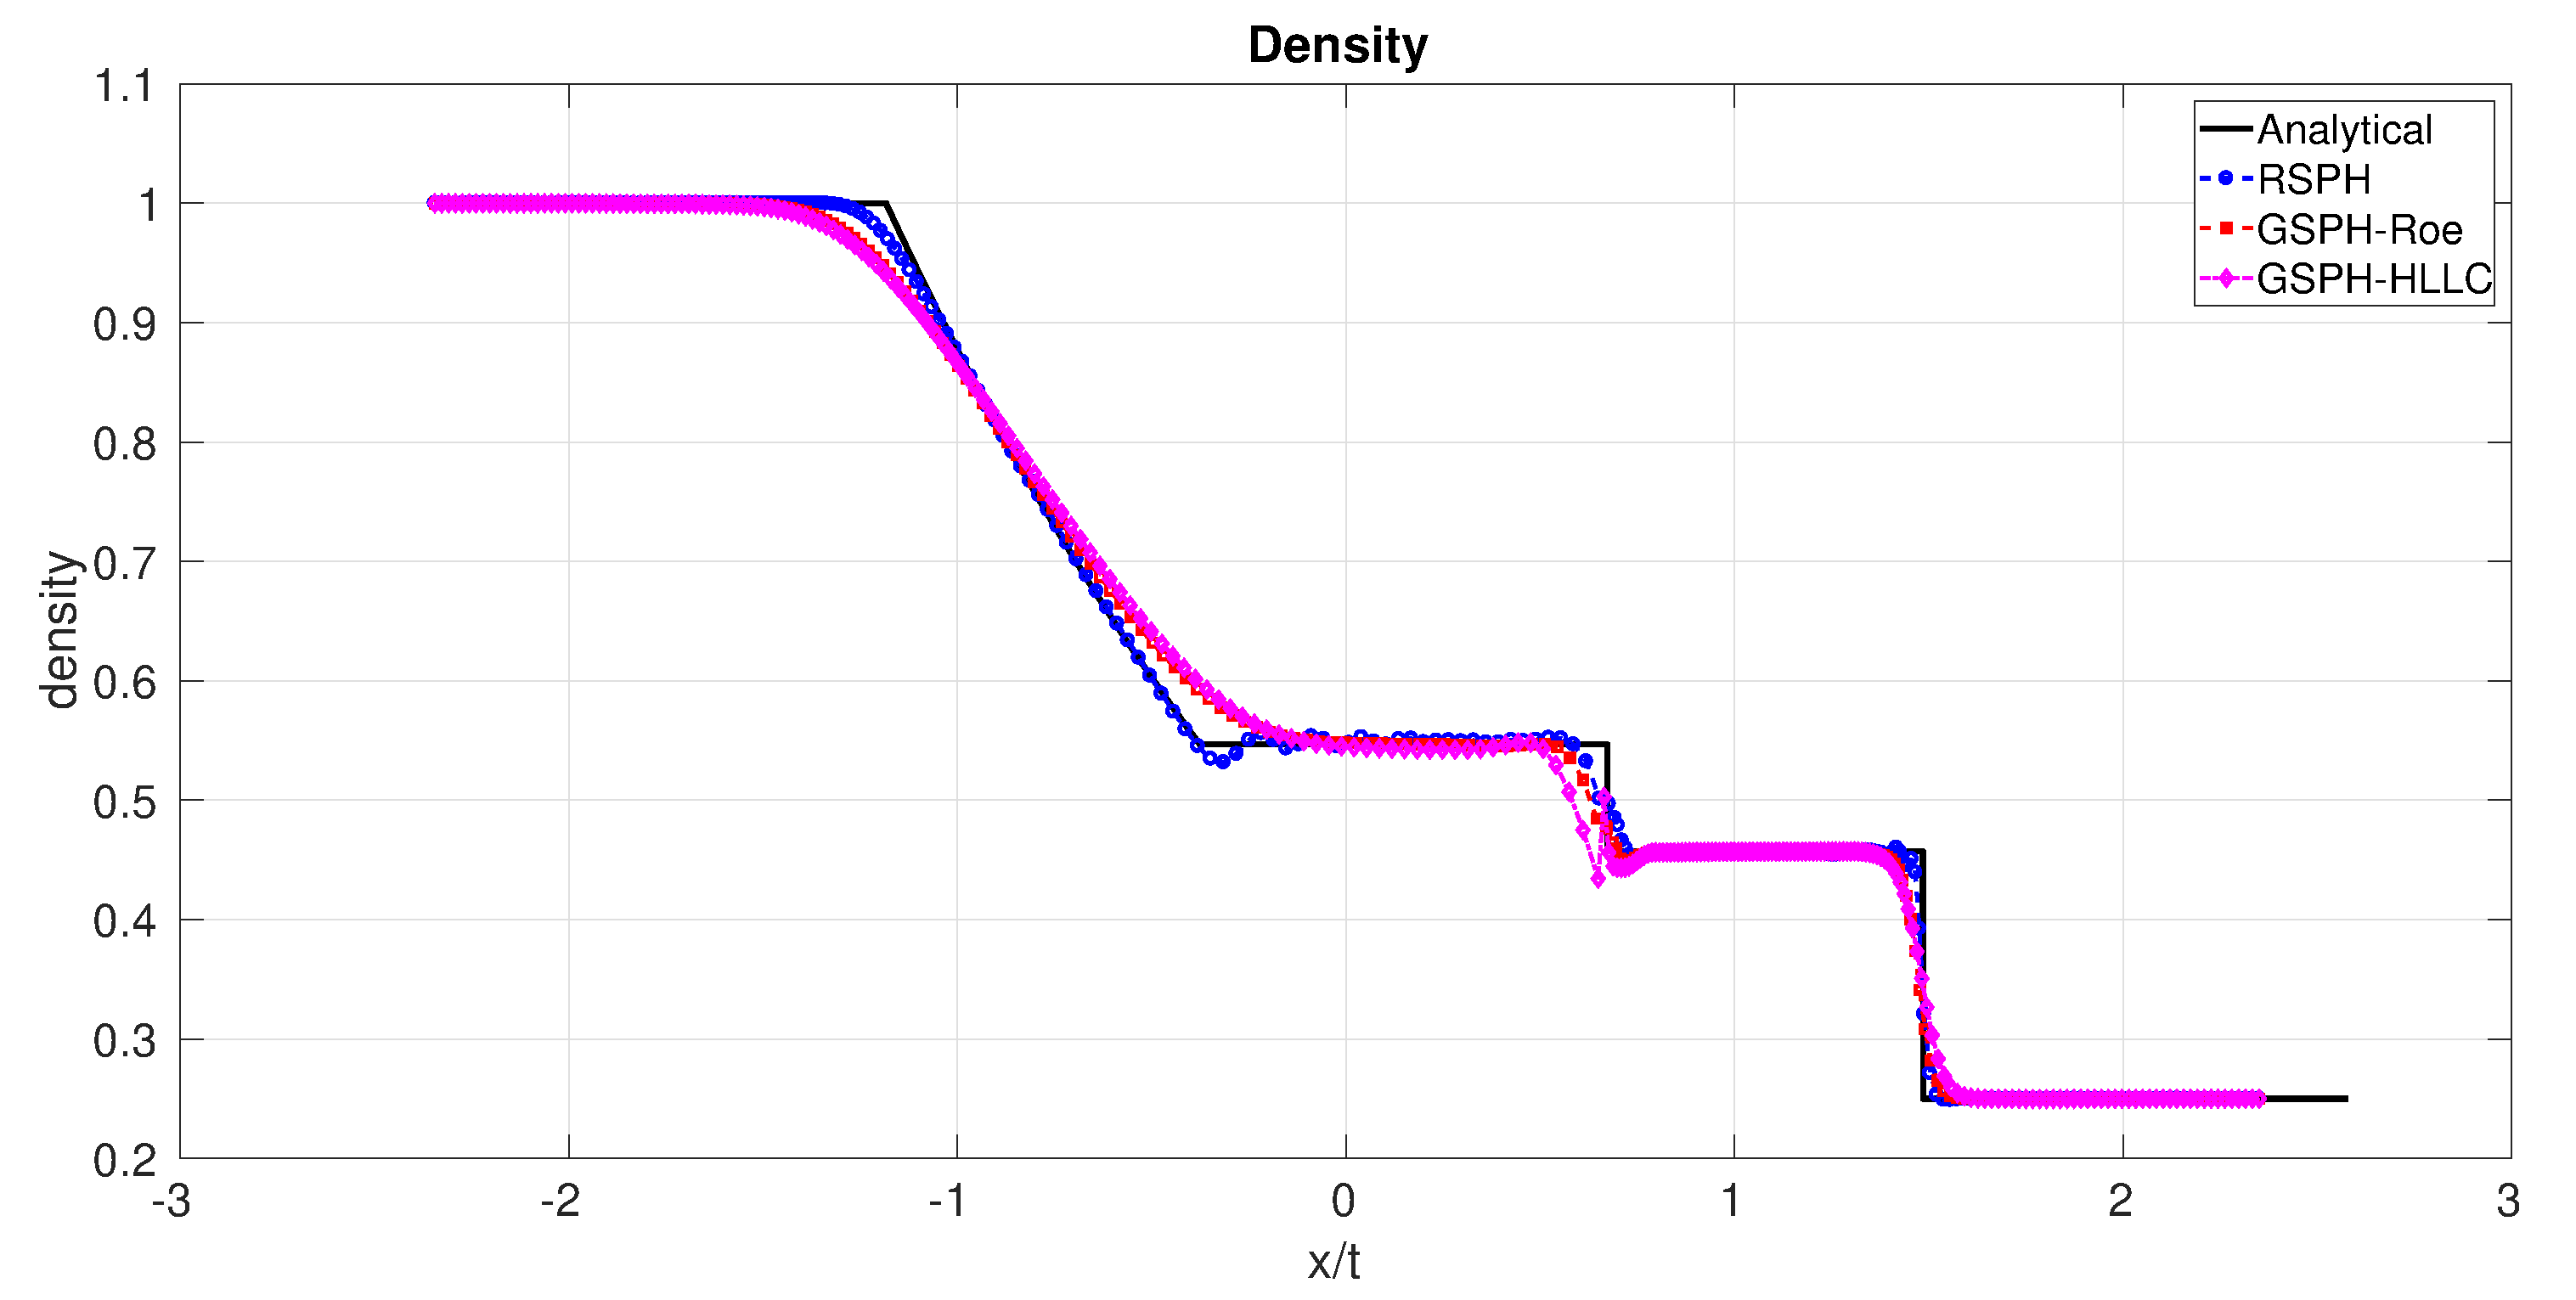
\includegraphics[width=0.99 \textwidth]{./Figures/Sod/RCM-Sod-GSPH-compare-rho}
    \end{minipage}%
    \begin{minipage}{.495 \textwidth}
        \centering
        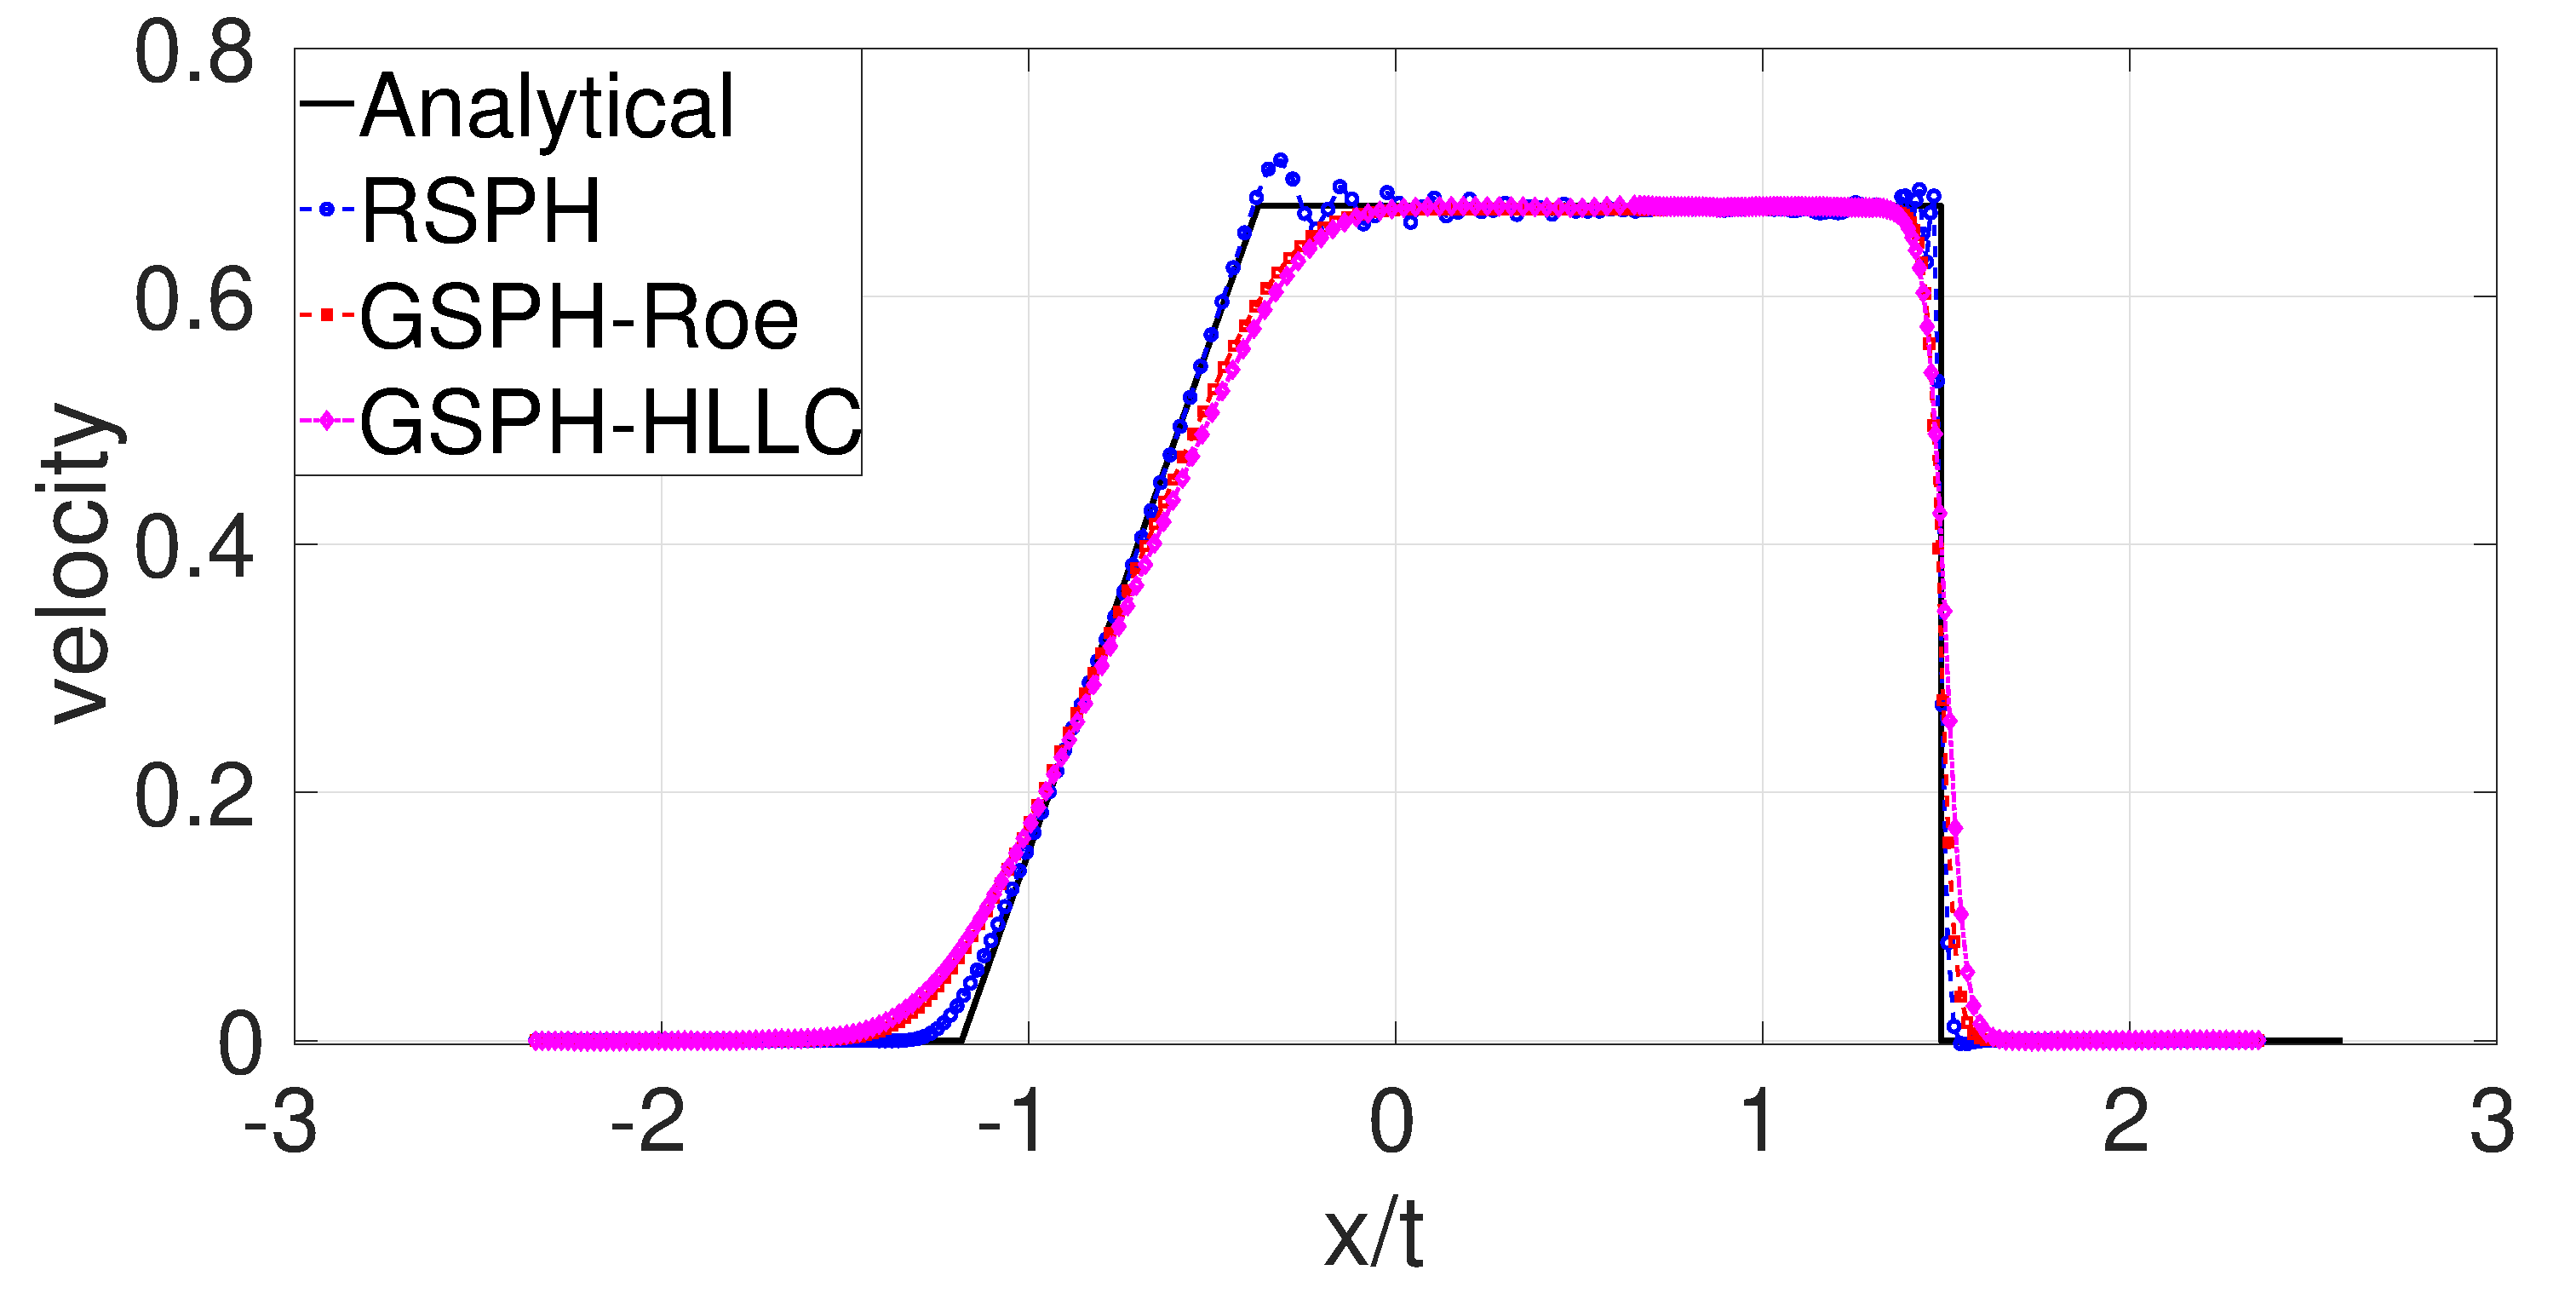
\includegraphics[width=0.99 \textwidth]{./Figures/Sod/RCM-Sod-GSPH-compare-v}
    \end{minipage}%
    \\
    \begin{minipage}{.495\textwidth}
        \centering
        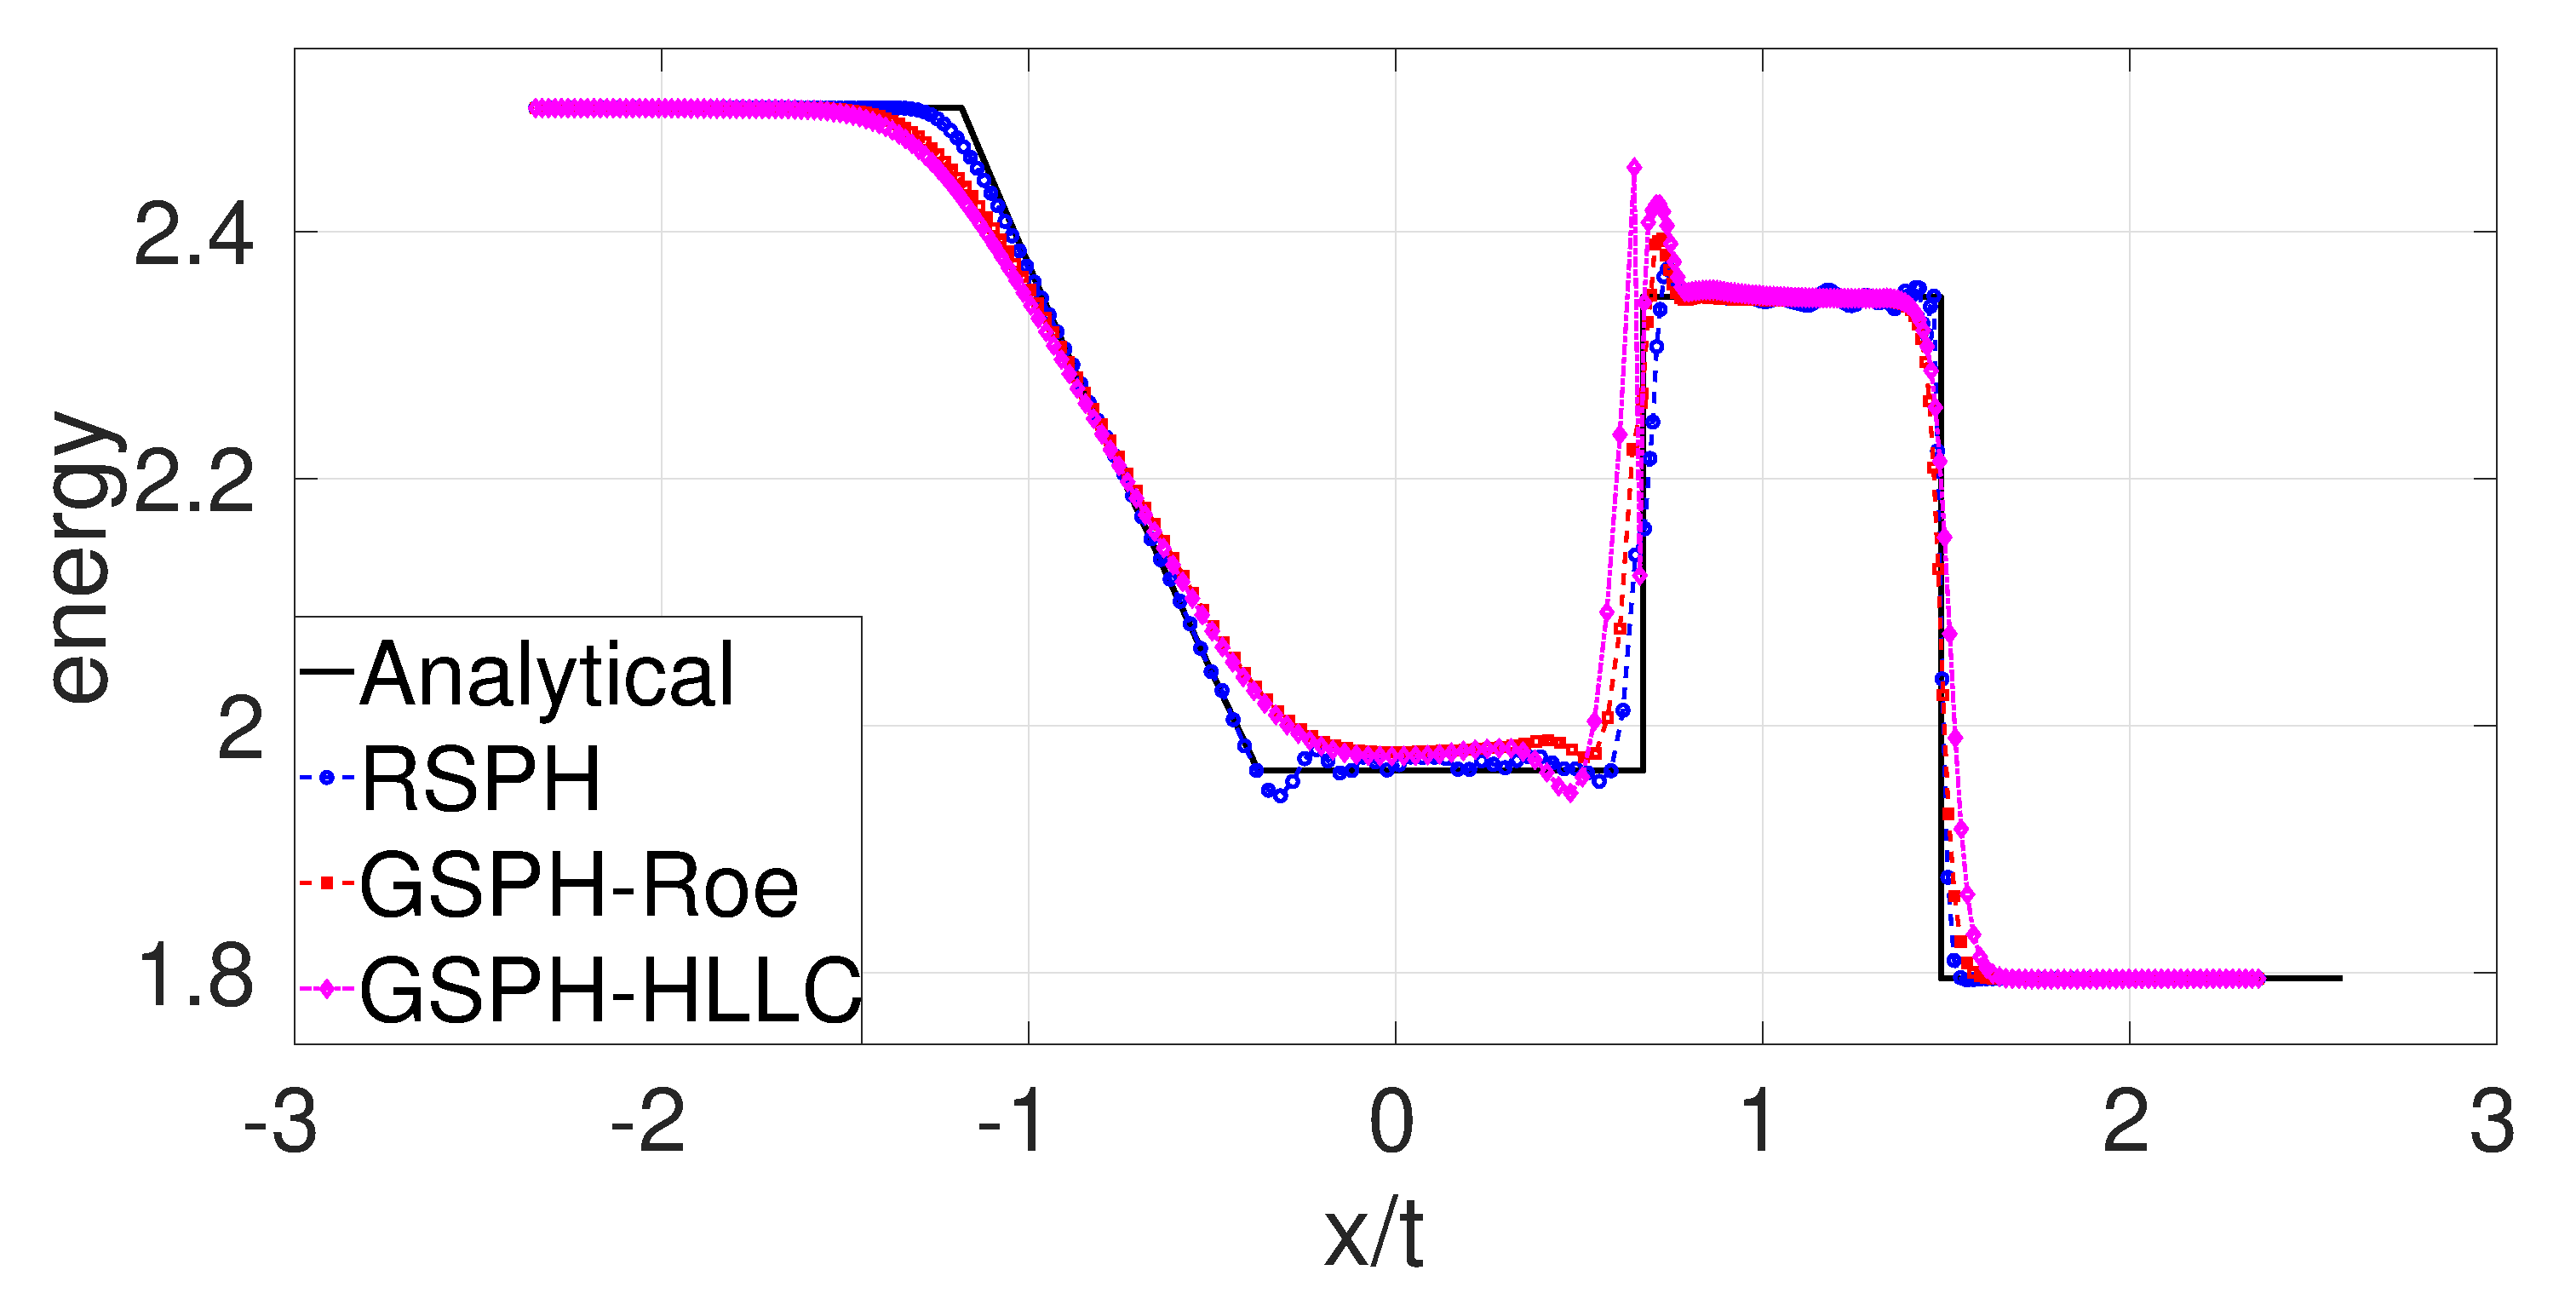
\includegraphics[width=0.99 \textwidth]{./Figures/Sod/RCM-Sod-GSPH-compare-e}
    \end{minipage}%
    \begin{minipage}{.495 \textwidth}
        \centering
        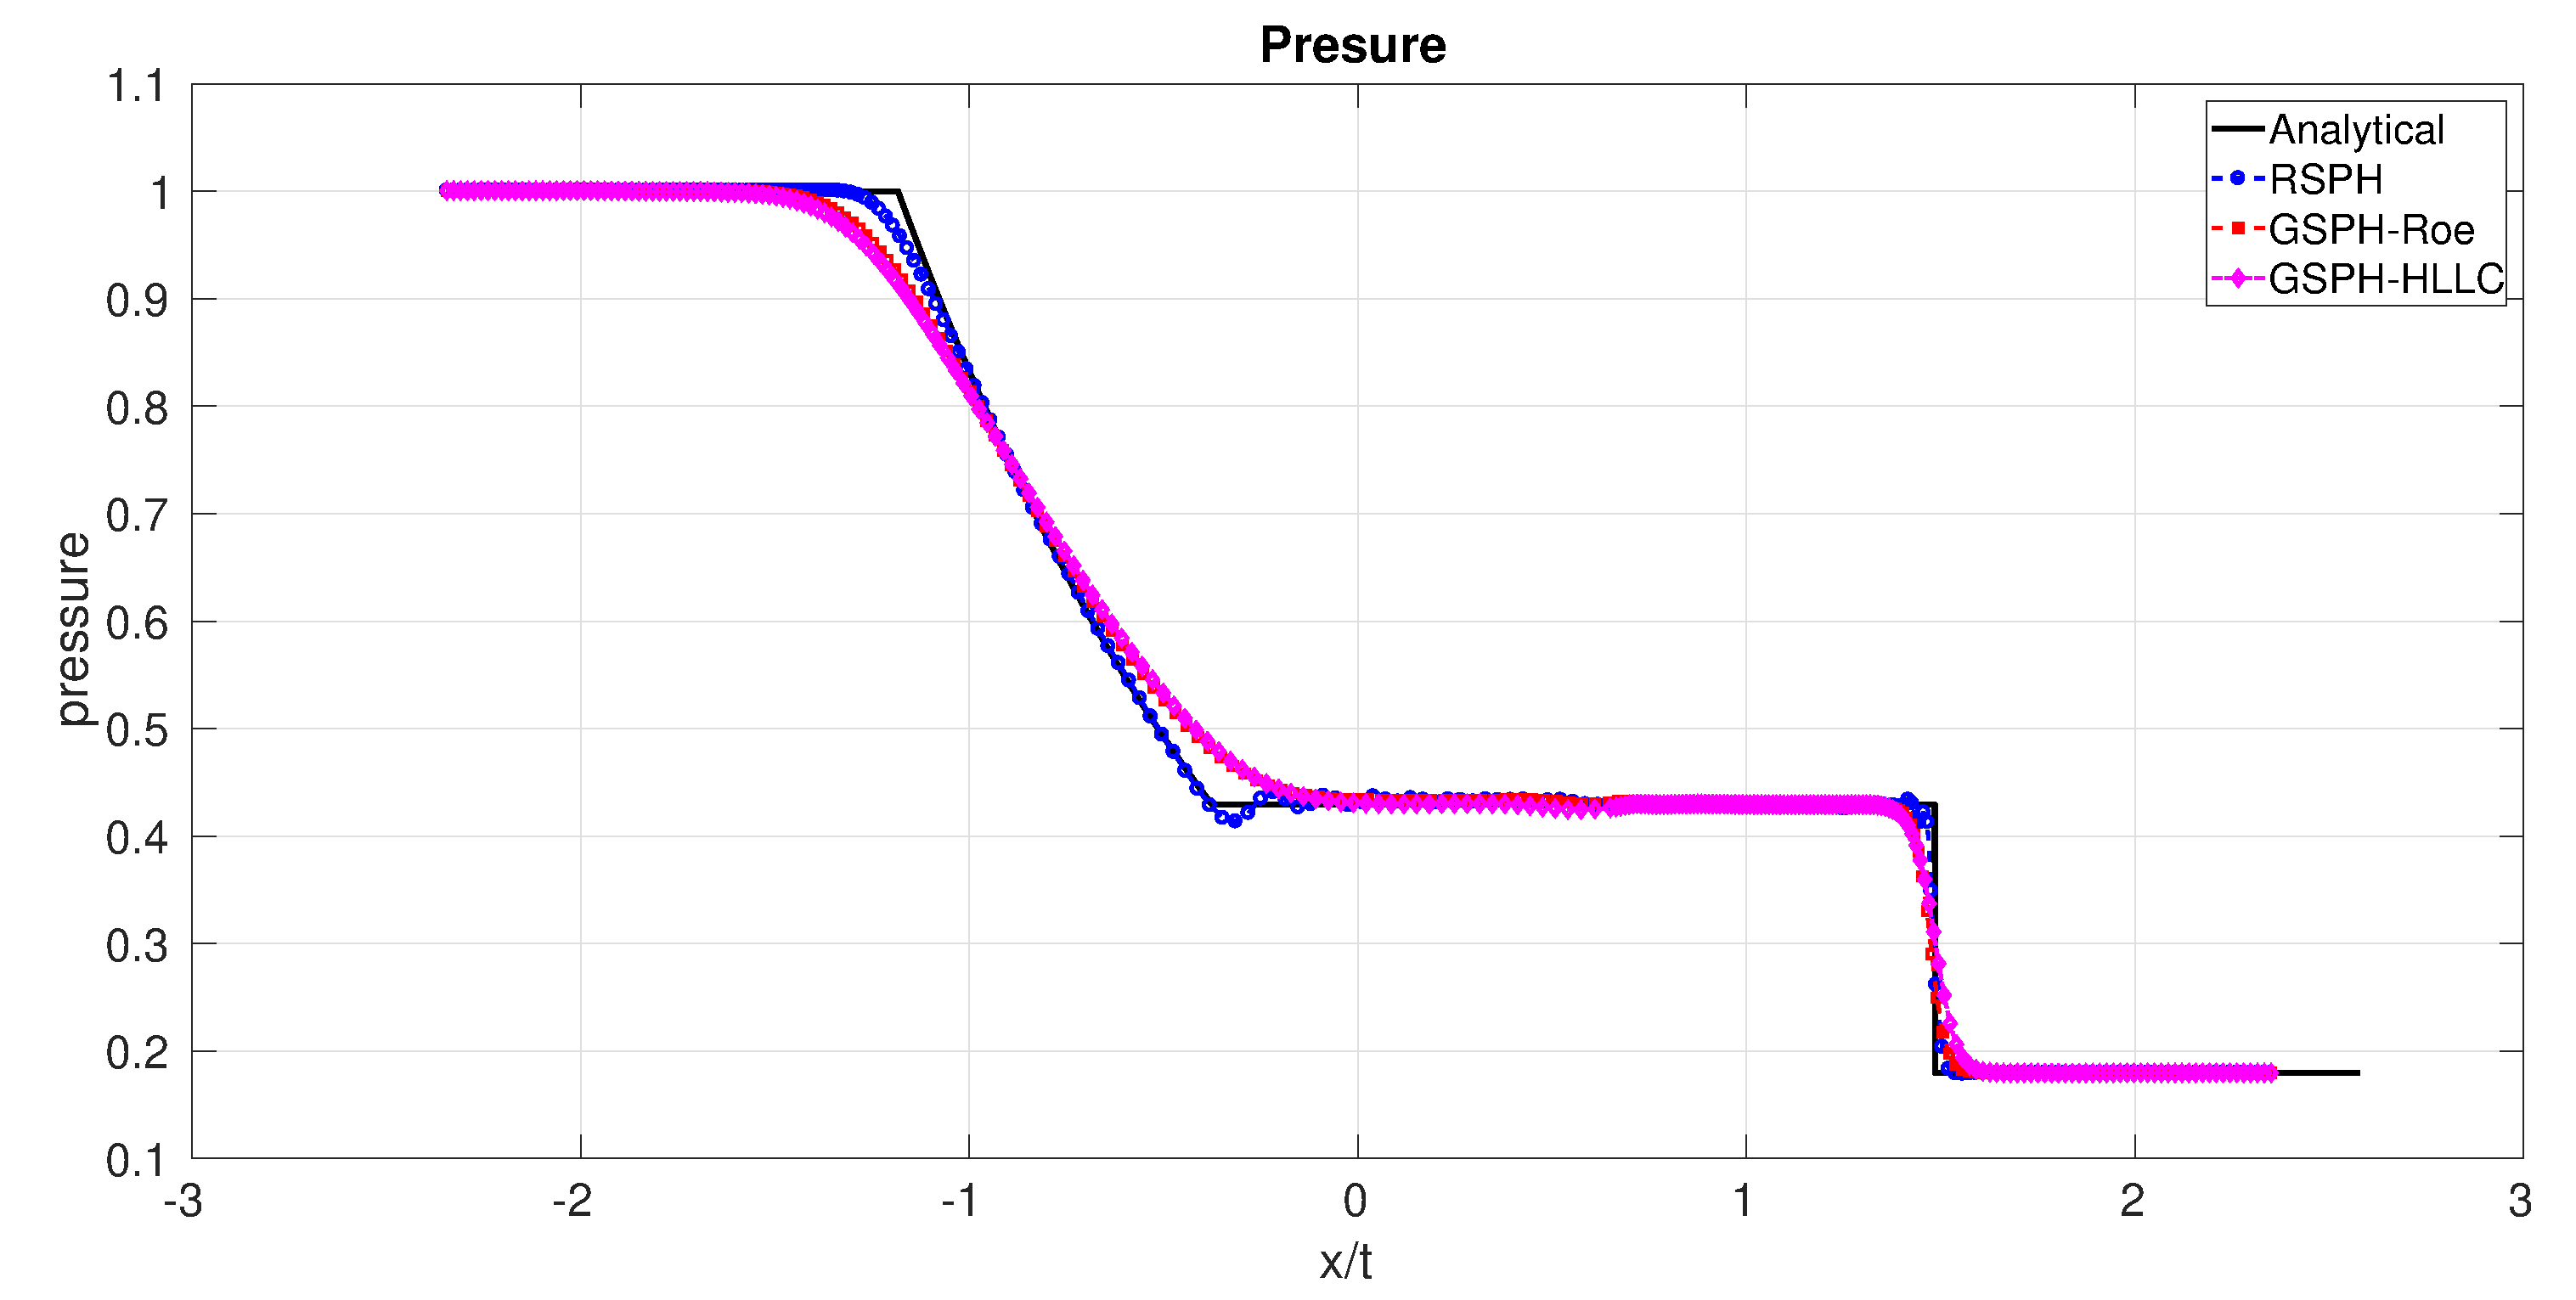
\includegraphics[width=0.99 \textwidth]{./Figures/Sod/RCM-Sod-GSPH-compare-p}
    \end{minipage}% 
    \\
    \begin{minipage}{.495\textwidth}
        \centering
        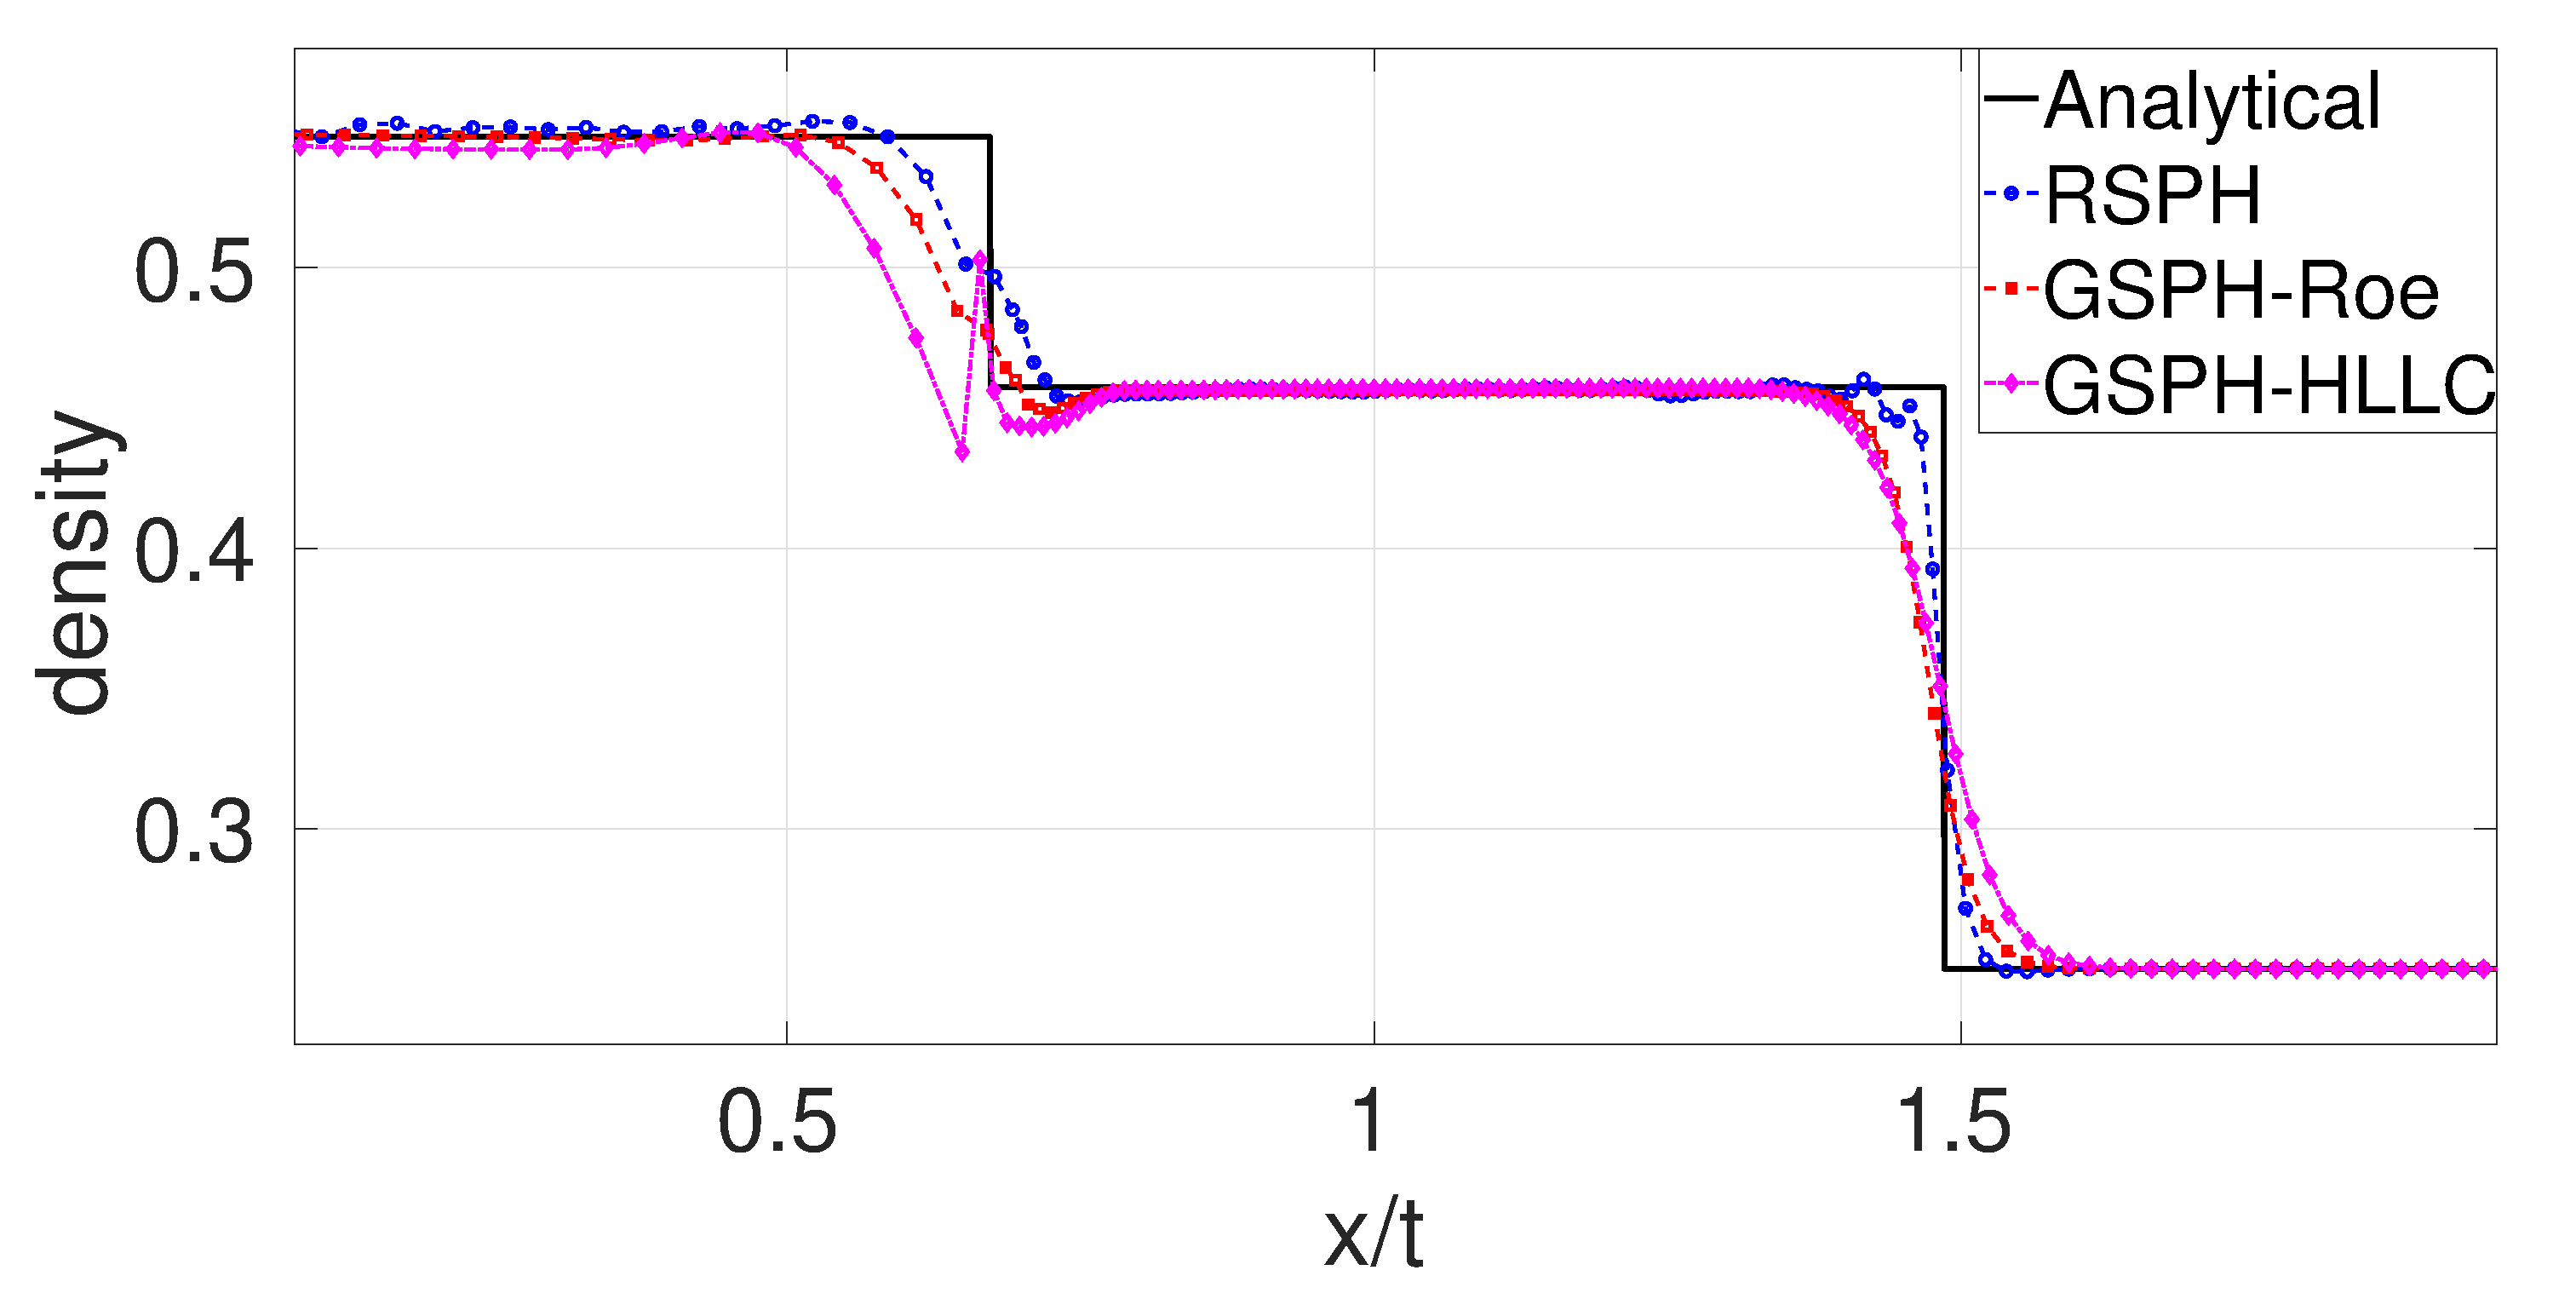
\includegraphics[width=0.99 \textwidth]{./Figures/Sod/RCM-Sod-GSPH-compare-rho-zoom}
    \end{minipage}%
    \begin{minipage}{.495 \textwidth}
        \centering
        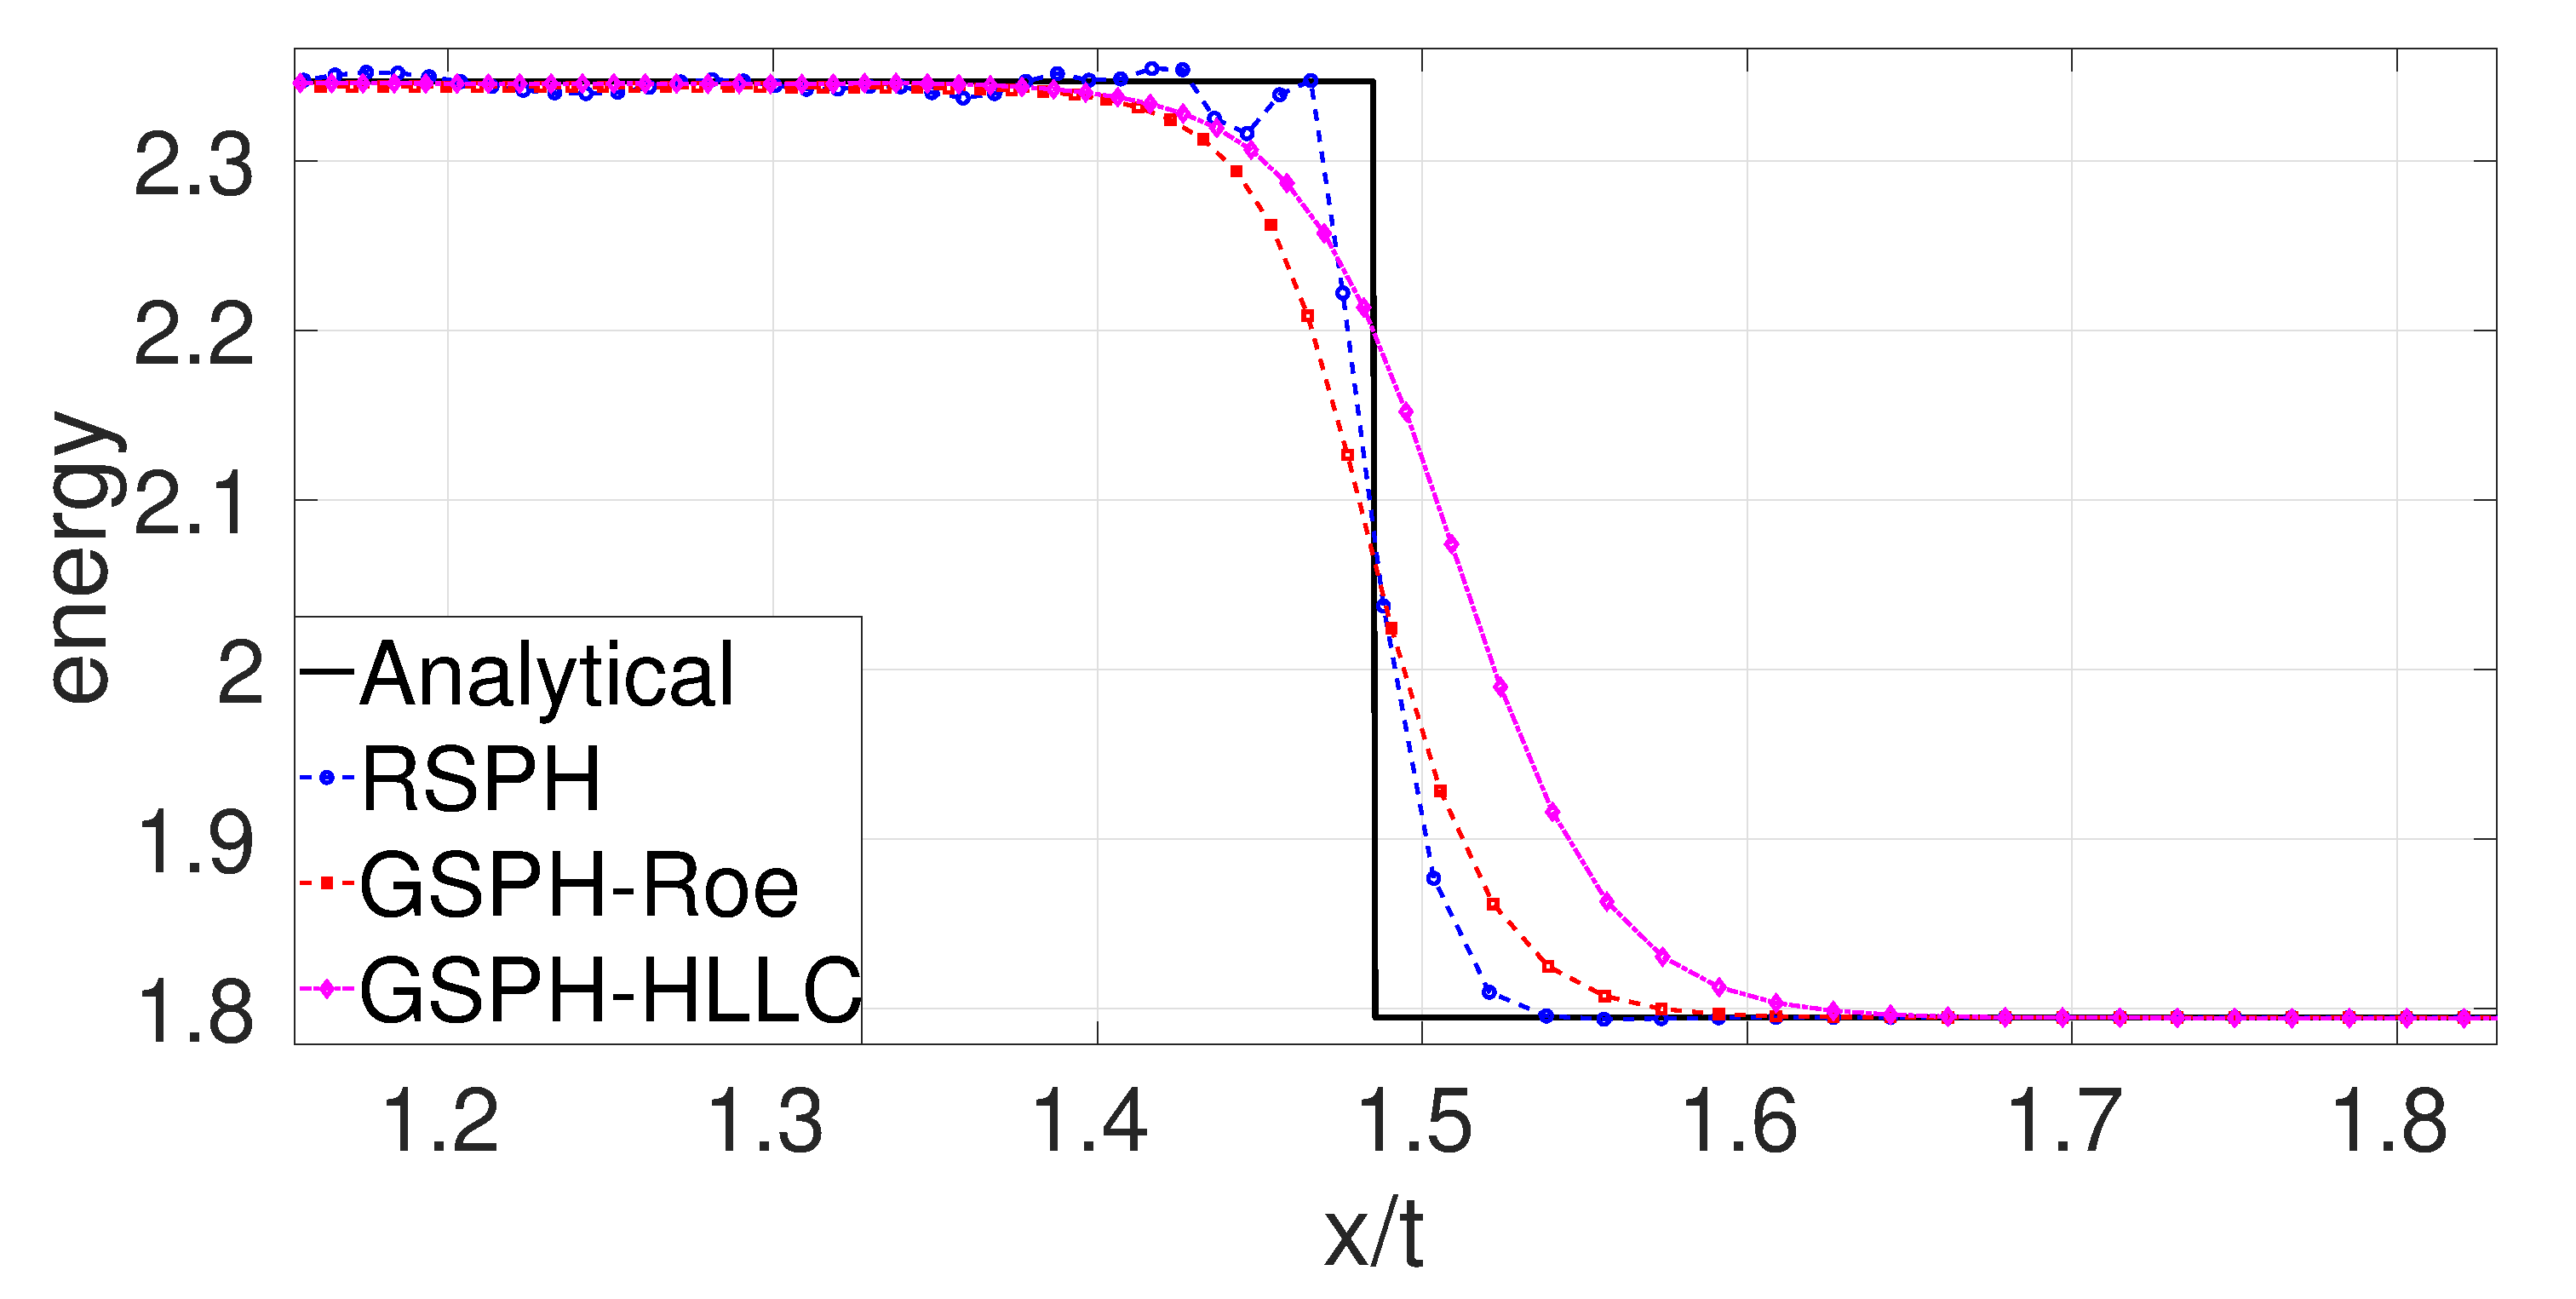
\includegraphics[width=0.99 \textwidth]{./Figures/Sod/RCM-Sod-GSPH-compare-e-zoom}
    \end{minipage}% 
    \\
    \begin{minipage}{.495 \textwidth}
        \centering
        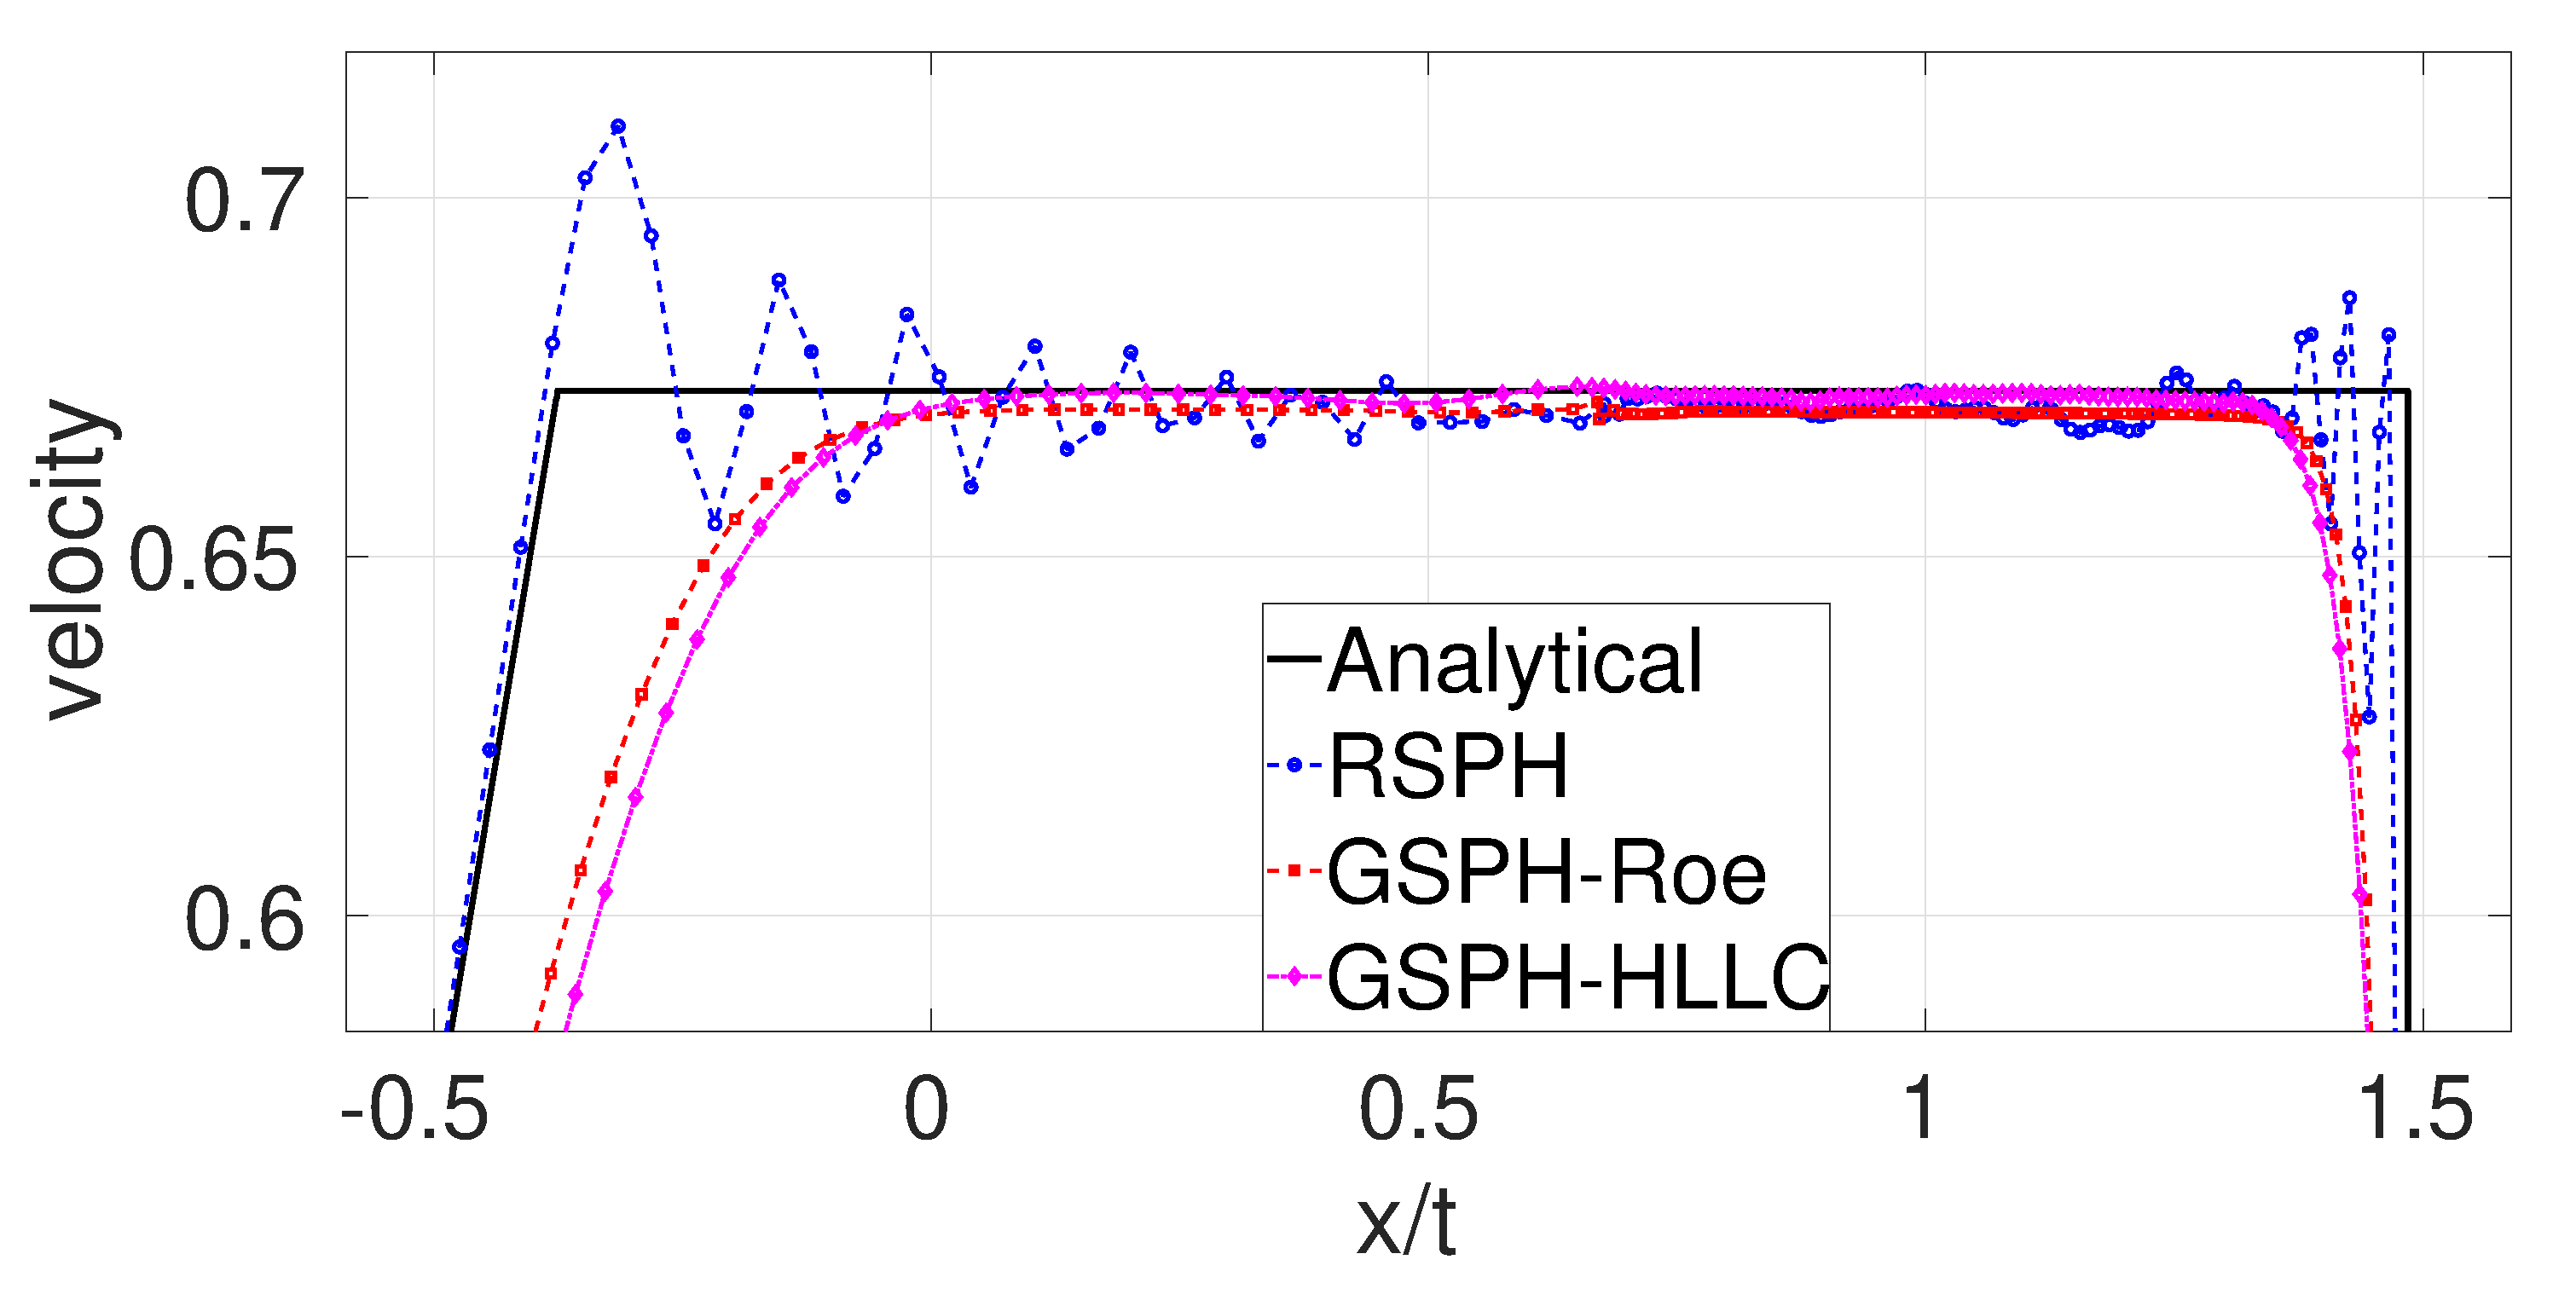
\includegraphics[width=0.99 \textwidth]{./Figures/Sod/RCM-Sod-GSPH-compare-v-zoom}
    \end{minipage}% 
    \begin{minipage}{.495\textwidth}
        \centering
        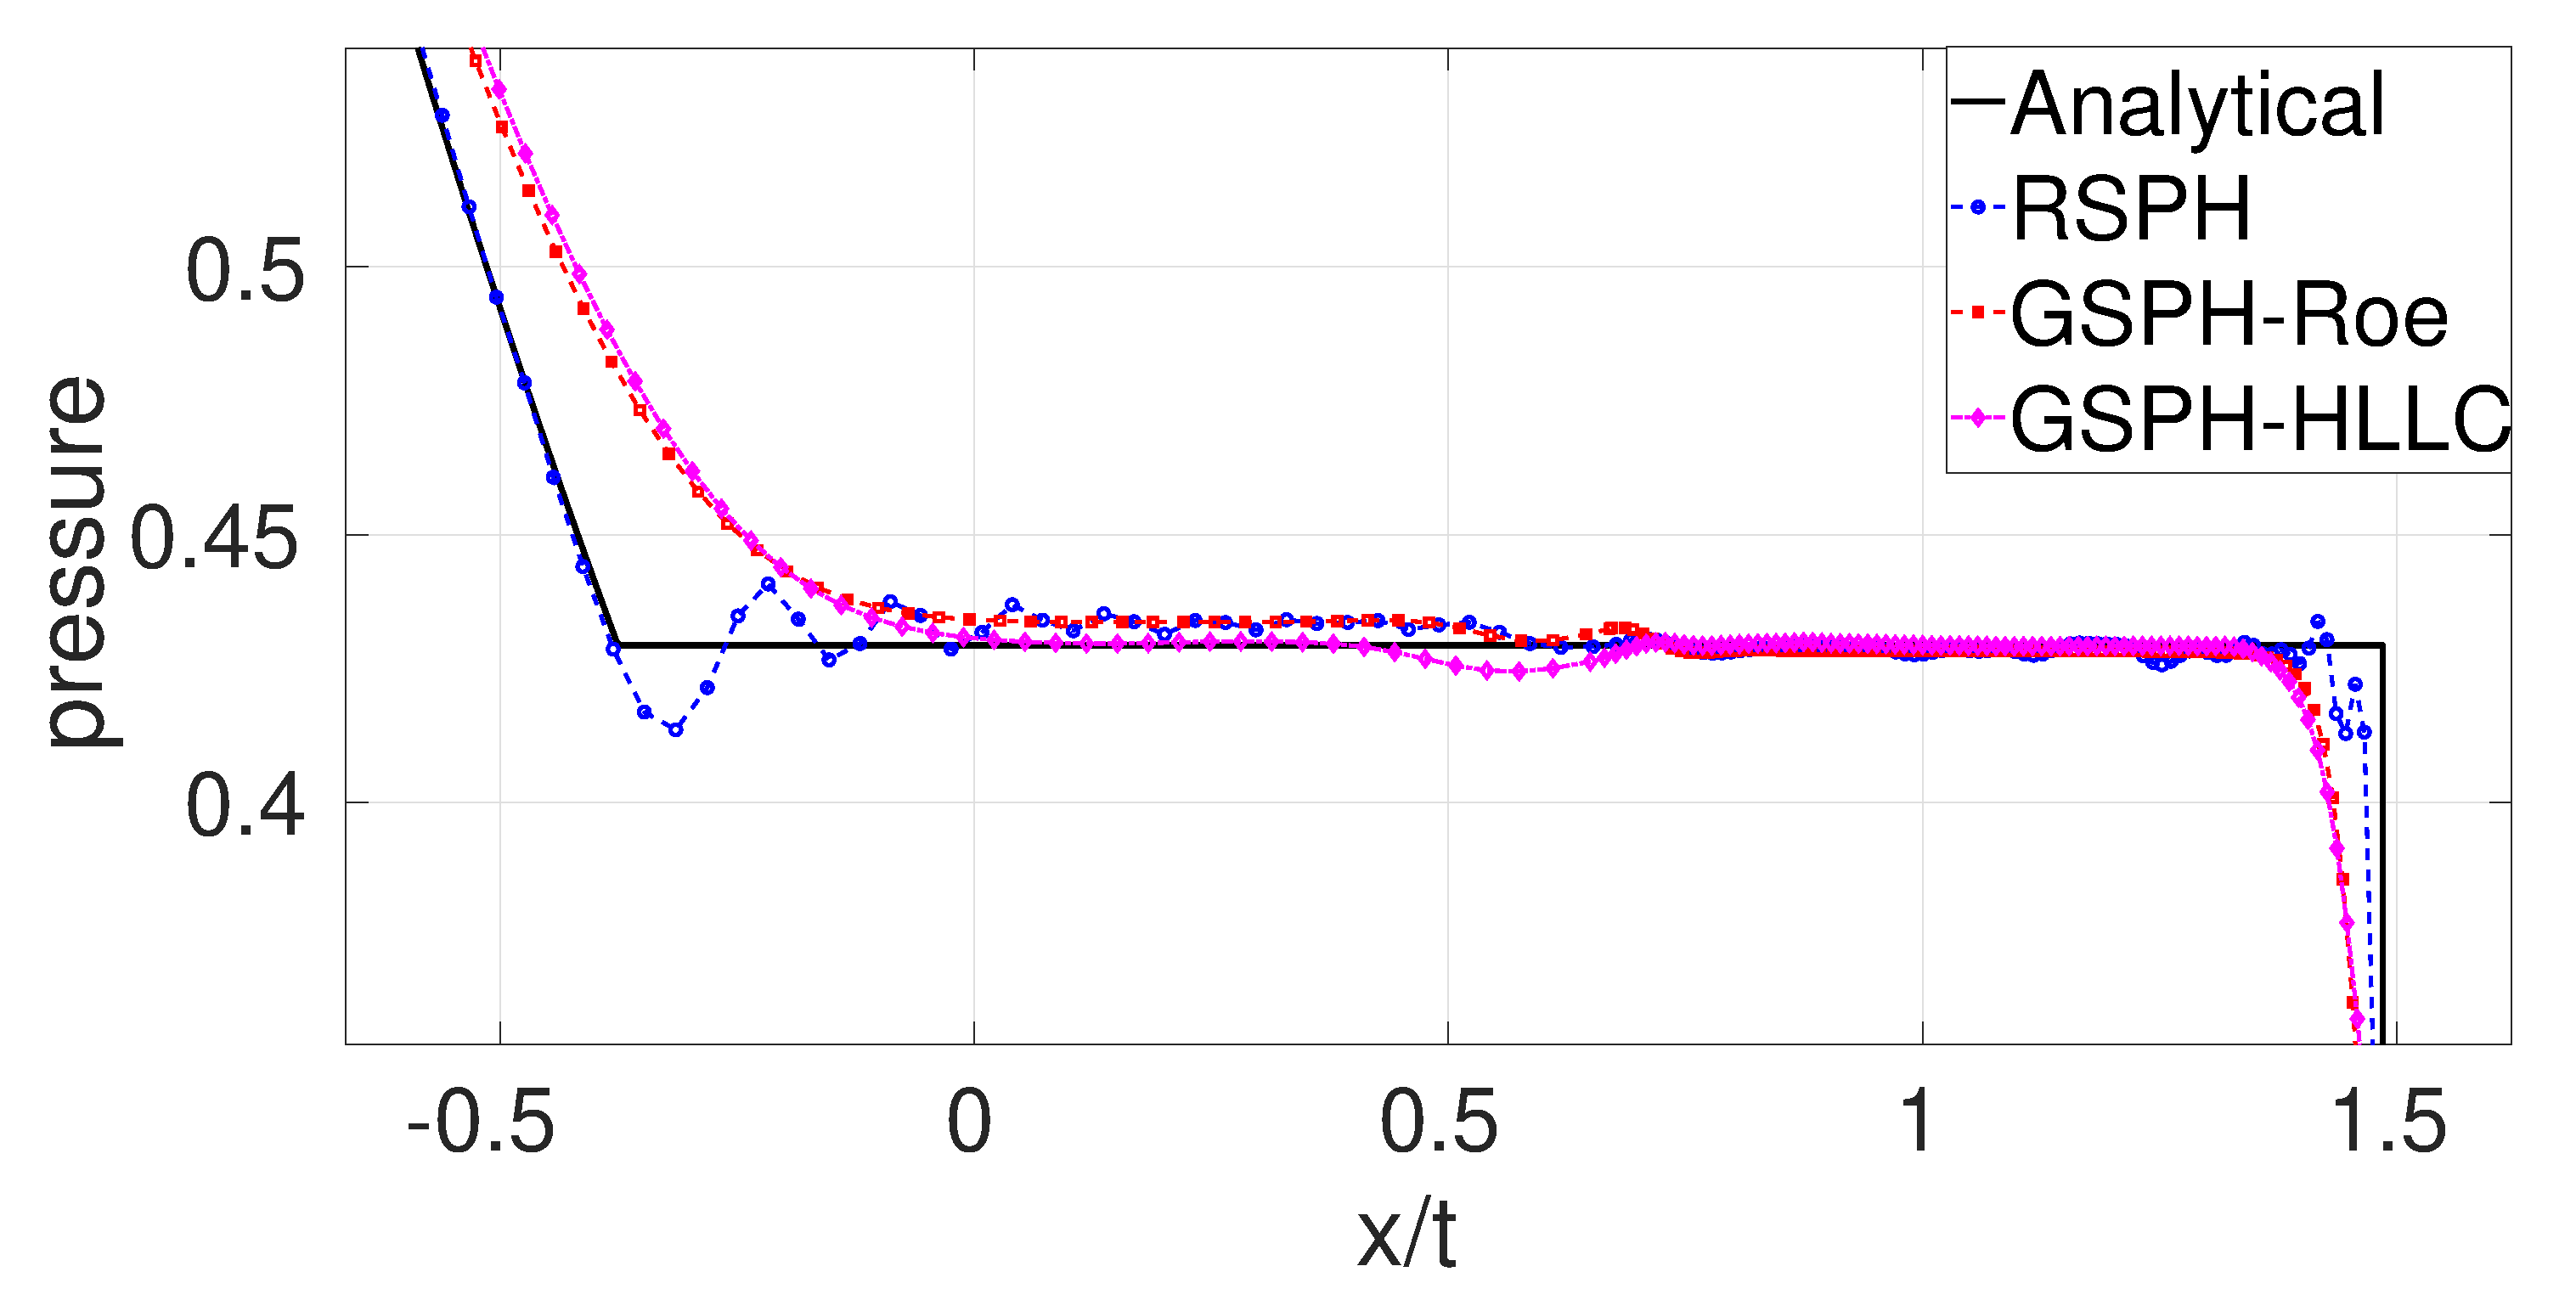
\includegraphics[width=0.99 \textwidth]{./Figures/Sod/RCM-Sod-GSPH-compare-p-zoom}
    \end{minipage}%    
    \caption{Comparison of RSPH with GSPH using Roe Riemann solver and HLLC Riemann solver. The last four plots are zoomed views. Zoomed view of density and specific internal energy show that GSPH smears the discontinuity at shock much more than RSPH. Zoomed view of velocity shows that fluctuation in GSPH is completely suppressed, which implies that numerical dissipation introduced in GSPH is at least around the same amount as SPH with $\alpha=1.0$. This is consistent with information implied by zoomed view of density and specific internal energy. The last zoomed view shows that both RSPH and GSPH can get rid of pressure ``wiggle" around the contact discontinuity.}
    \label{fig:RCM-Sod-GSPH}
\end{figure}

These zoomed views in fig. \ref{fig:RCM-Sod-GSPH} demonstrate that RSPH introduces less but sufficient dissipation compared with GSPH. The attractive feature of RCM method in preserving true discontinuity is inherited by RSPH in this 1D shock tube test. With more dissipation, GSPH can completely suppress numerical dissipation. The discontinuity at the shock is more seriously smeared. The excessive amount dissipation might have other, more undesirable, effects in real implementation. For example, over damping of shearing flow. Compared with SPH, both GSPH and RSPH avoid pressure ``wiggle" around contact discontinuity. Since RSPH share many common places with Godunov's method, it is not surprise that RSPH can also suppress the pressure ``wiggle" at contact discontinuity.

\subsection{Accuracy tests}
We use shock tube test to gauge the accuracy of the RSPH scheme.
% for both situations when the solution remains smooth and when there are shocks in the solution. We use test 1 to conduct order of accuracy test for the case with shocks in the solution. 
We examine the errors between simulation results and the analytical solution (the reference solution) as the number of particles is increased. The $L_1$ norm error, defined for a property $f$, is normalized by the number of particles as:
\begin{equation}
L_1= \frac{1}{N_p} \sum_a^{N_p} \vert f_a^{SPH} - f^{REF} (x_a) \vert 
\end{equation}
where the superscript $REF$ represent the reference solution, $SPH$ represents simulation results calculated by different SPH schemes. Fig. \ref{fig:Accuracy-test1} displays the $L_1$ norm errors for the density, velocity and pressure profiles for different SPH schemes.
We observe a rate of convergence of approximately 1 for GSPH and 1.5 for standard SPH and RSPH.
GSPH with an exact Riemann solver has been shown to be approximately second order of accuracy \citep{puri2014comparison} and comparable in accuracy to the standard SPH schemes when using piece wise linear construction. As for GSPH using approximate Riemann solver, \citet{puri2014approximate} reported second order accuracy for HLLC and Roe Riemann solvers adopting piece wise linear Riemann problem construction. In addition, they adopted a test problem without discontinuity in the solution. Existing of discontinuities, such as shock, in the test problem might lower rate of convergence. Both RSPH and GSPH tests in this paper adopt a piece wise constant construction of Riemann problem. So we conclude that RSPH shows higher order of accuracy than GSPH when using the same Riemann problem construction. Compared with SPH, RSPH shows almost the same order of accuracy and level of error.
%It is worthwhile to check the order of accuracy of GSPH using piecewise linear constructor
%It is also worthwile to check what of order of accuracy using another test problem.  
\begin{figure}[H]
    \centering
    \begin{minipage}{.332\textwidth}
        \centering
        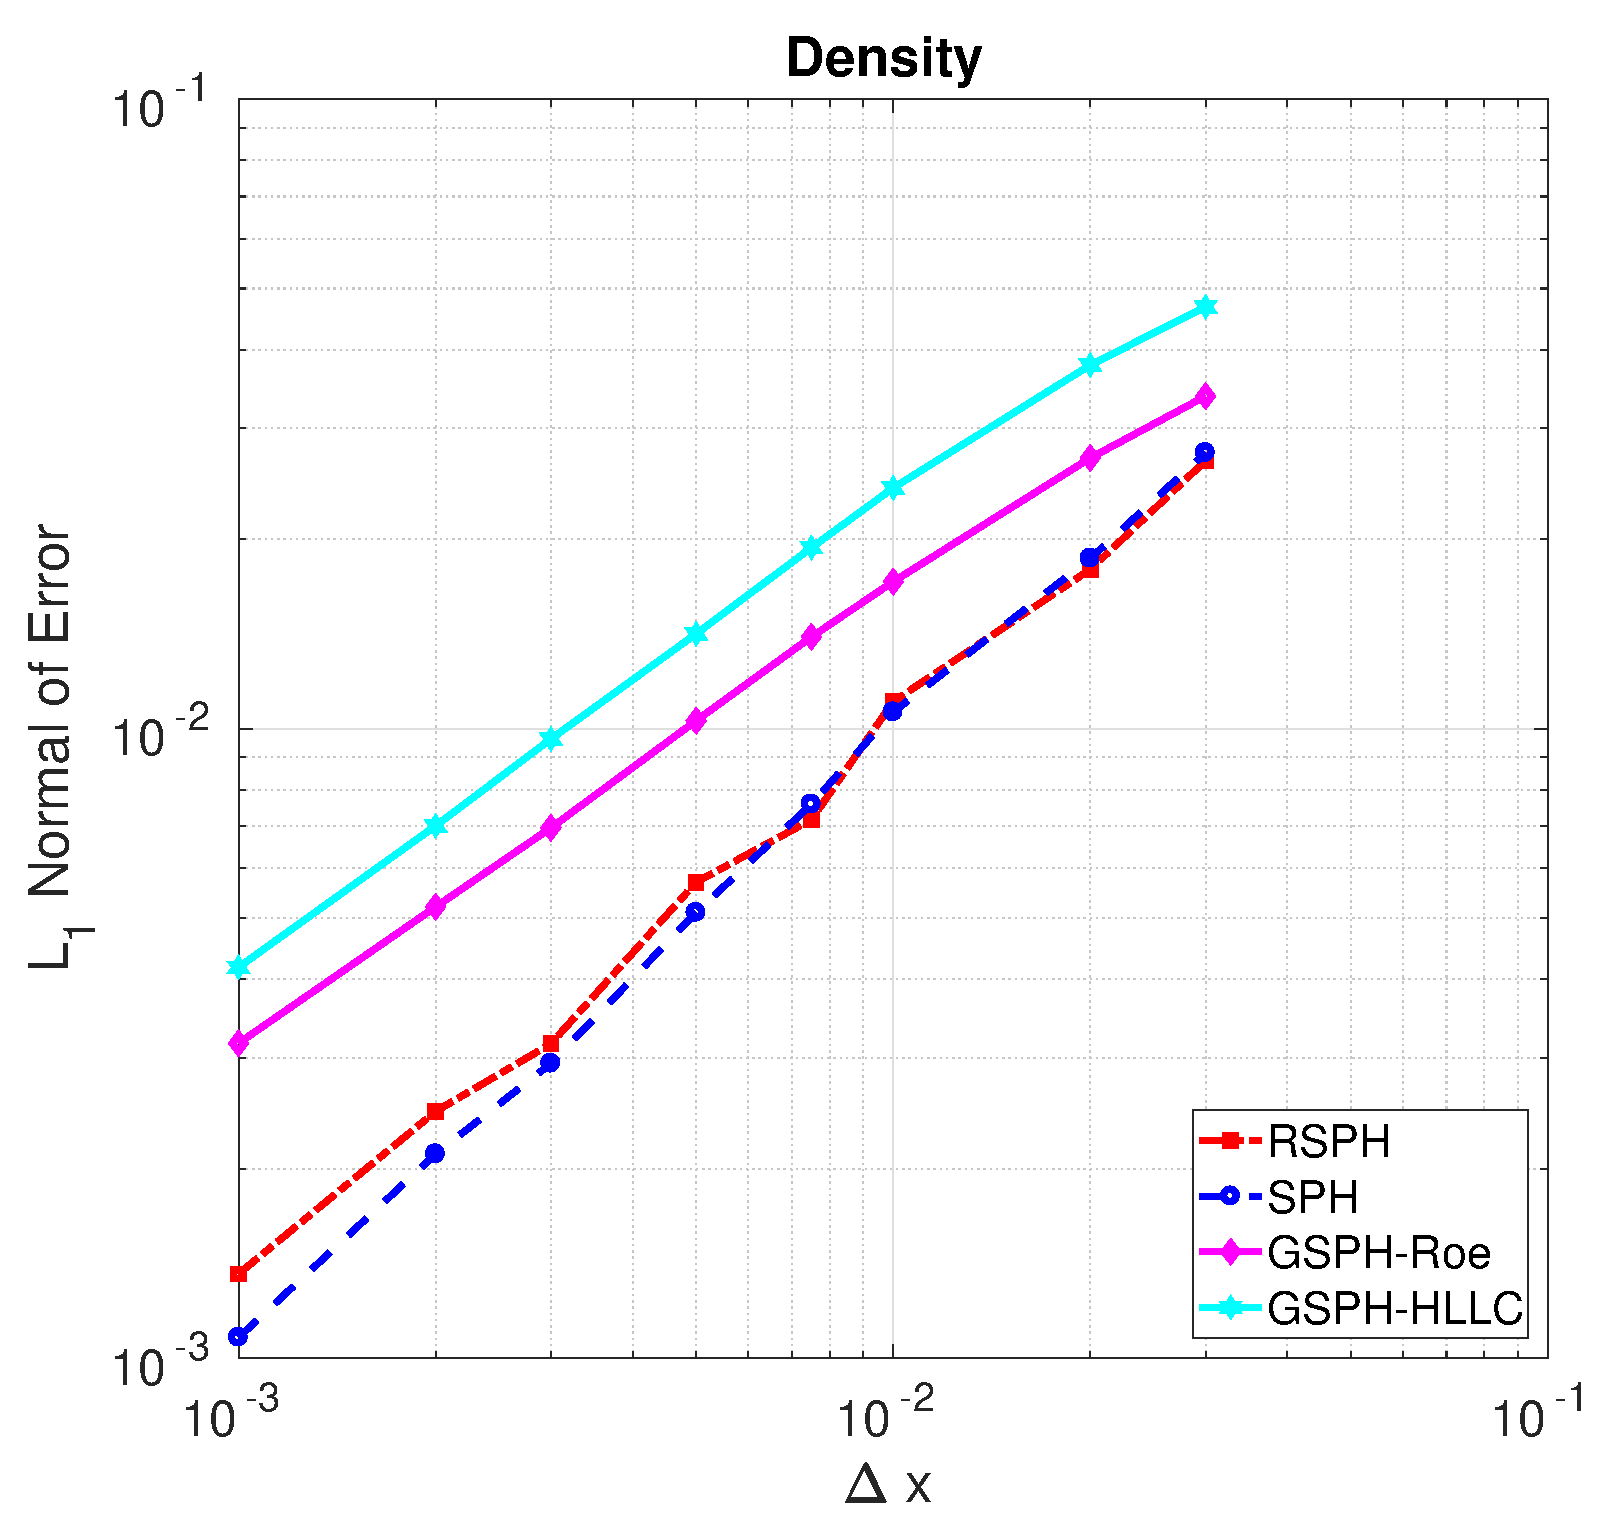
\includegraphics[width=0.99 \textwidth]{./Figures/Accuracy-des}
    \end{minipage}%
    \begin{minipage}{.332 \textwidth}
        \centering
        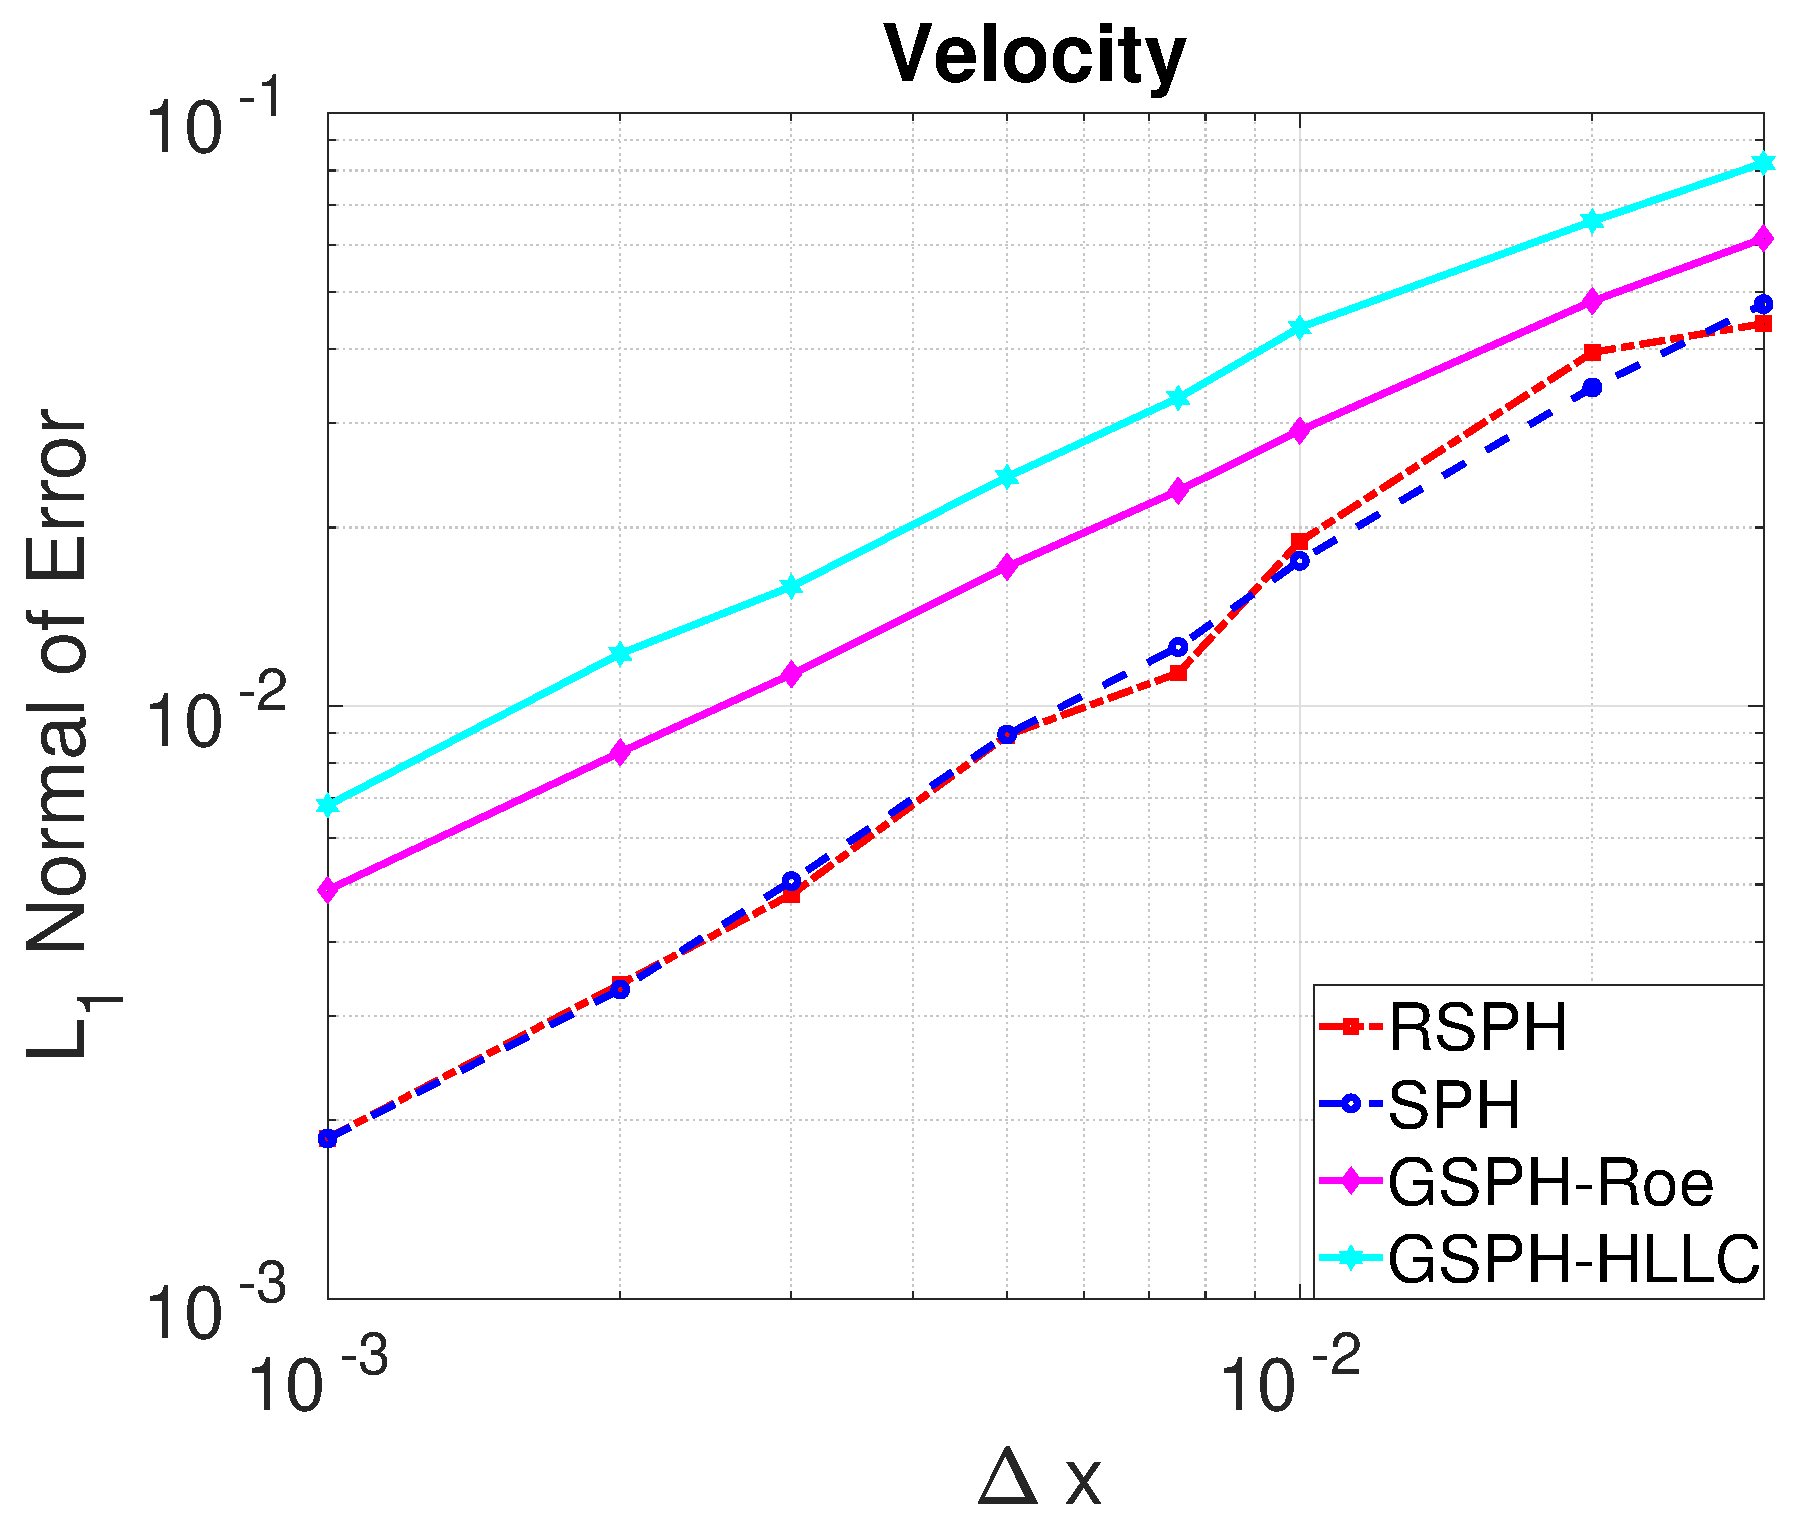
\includegraphics[width=0.99 \textwidth]{./Figures/Accuracy-vel}
    \end{minipage}%
    \begin{minipage}{.332\textwidth}
        \centering
        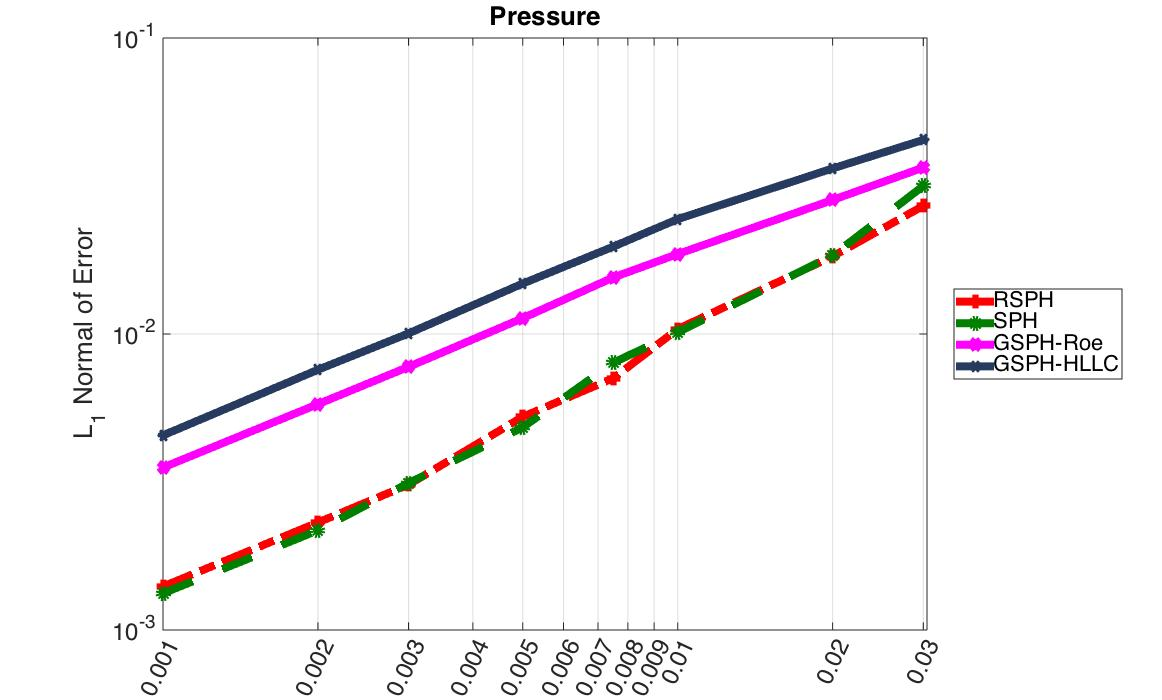
\includegraphics[width=0.99 \textwidth]{./Figures/Accuracy-pre}
    \end{minipage}%  
    \caption{ $L_1$ norm errors for 1D shock tube test (test1) for RSPH, standard SPH, GSPH using Roe Riemann solver and GSPH using HLLC Riemann Solver.  GSPH with the HLLC approximate Riemann solver exhibits the same convergence rate (around 1) but quantitatively larger errors than that with Roe Riemann solver. RSPH and standard SPH shows same rate of convergence and almost same amount of error.}
    \label{fig:Accuracy-test1}
\end{figure}
 
\subsection{Comprehensive 1D tests} \label{sec:comprehensive-1d-tests}
Comprehensive tests are presented in this section to check how well does RSPH work for different situations. Input parameters for each tests is given in Table \ref{tab:1D-shock-input_parameters}. Wave speed is estimated based on formulation Eq. (\ref{eq:RP-solver-HLLC-SM}) $\sim$ Eq. (\ref{eq:RP-solver-HLLC-SR}).
The results are shown in Fig. \ref{fig:RCM-GSPH-Sod} $\sim$ Fig. \ref{fig:RCM-strong-blast}. $x$ axis in these plots are normalized by the terminal time $t_f$. We observe that RSPH is able to correctly predict the position and magnitude of all waves for all tests. A jump of specific internal energy at the origin is observed in Sjogreen test. However, such jump is a common issue of SPH schemes and has been reported in many other tests (see, for example, \citep{monaghan1997sph,cha2003implementations,puri2014approximate})
In addition, a noticeable spike can be observed near the contact discontinuity. Similar spike is observed in GSPH simulation \citep{puri2014comparison}. Such spike is evident in the FVM solution as well and is perhaps an artifice of the Lagrangian nature of the two schemes. \citep{noh1987errors} proposed to adding a small amount of thermal conduction to ameliorate the spike and has been applied in blast-wave test using GSPH \citep{puri2014comparison}. We did not adopt such strategy in our simulation.
Due to less amount of dissipation, numerical fluctuations persist in all simulation results. For the strong blast test and double shock test, such fluctuations become more obvious than other tests. Even though, the magnitude of fluctuations is within acceptable range.

\begin{figure}[H]
    \centering
    \begin{minipage}{.495\textwidth}
        \centering
        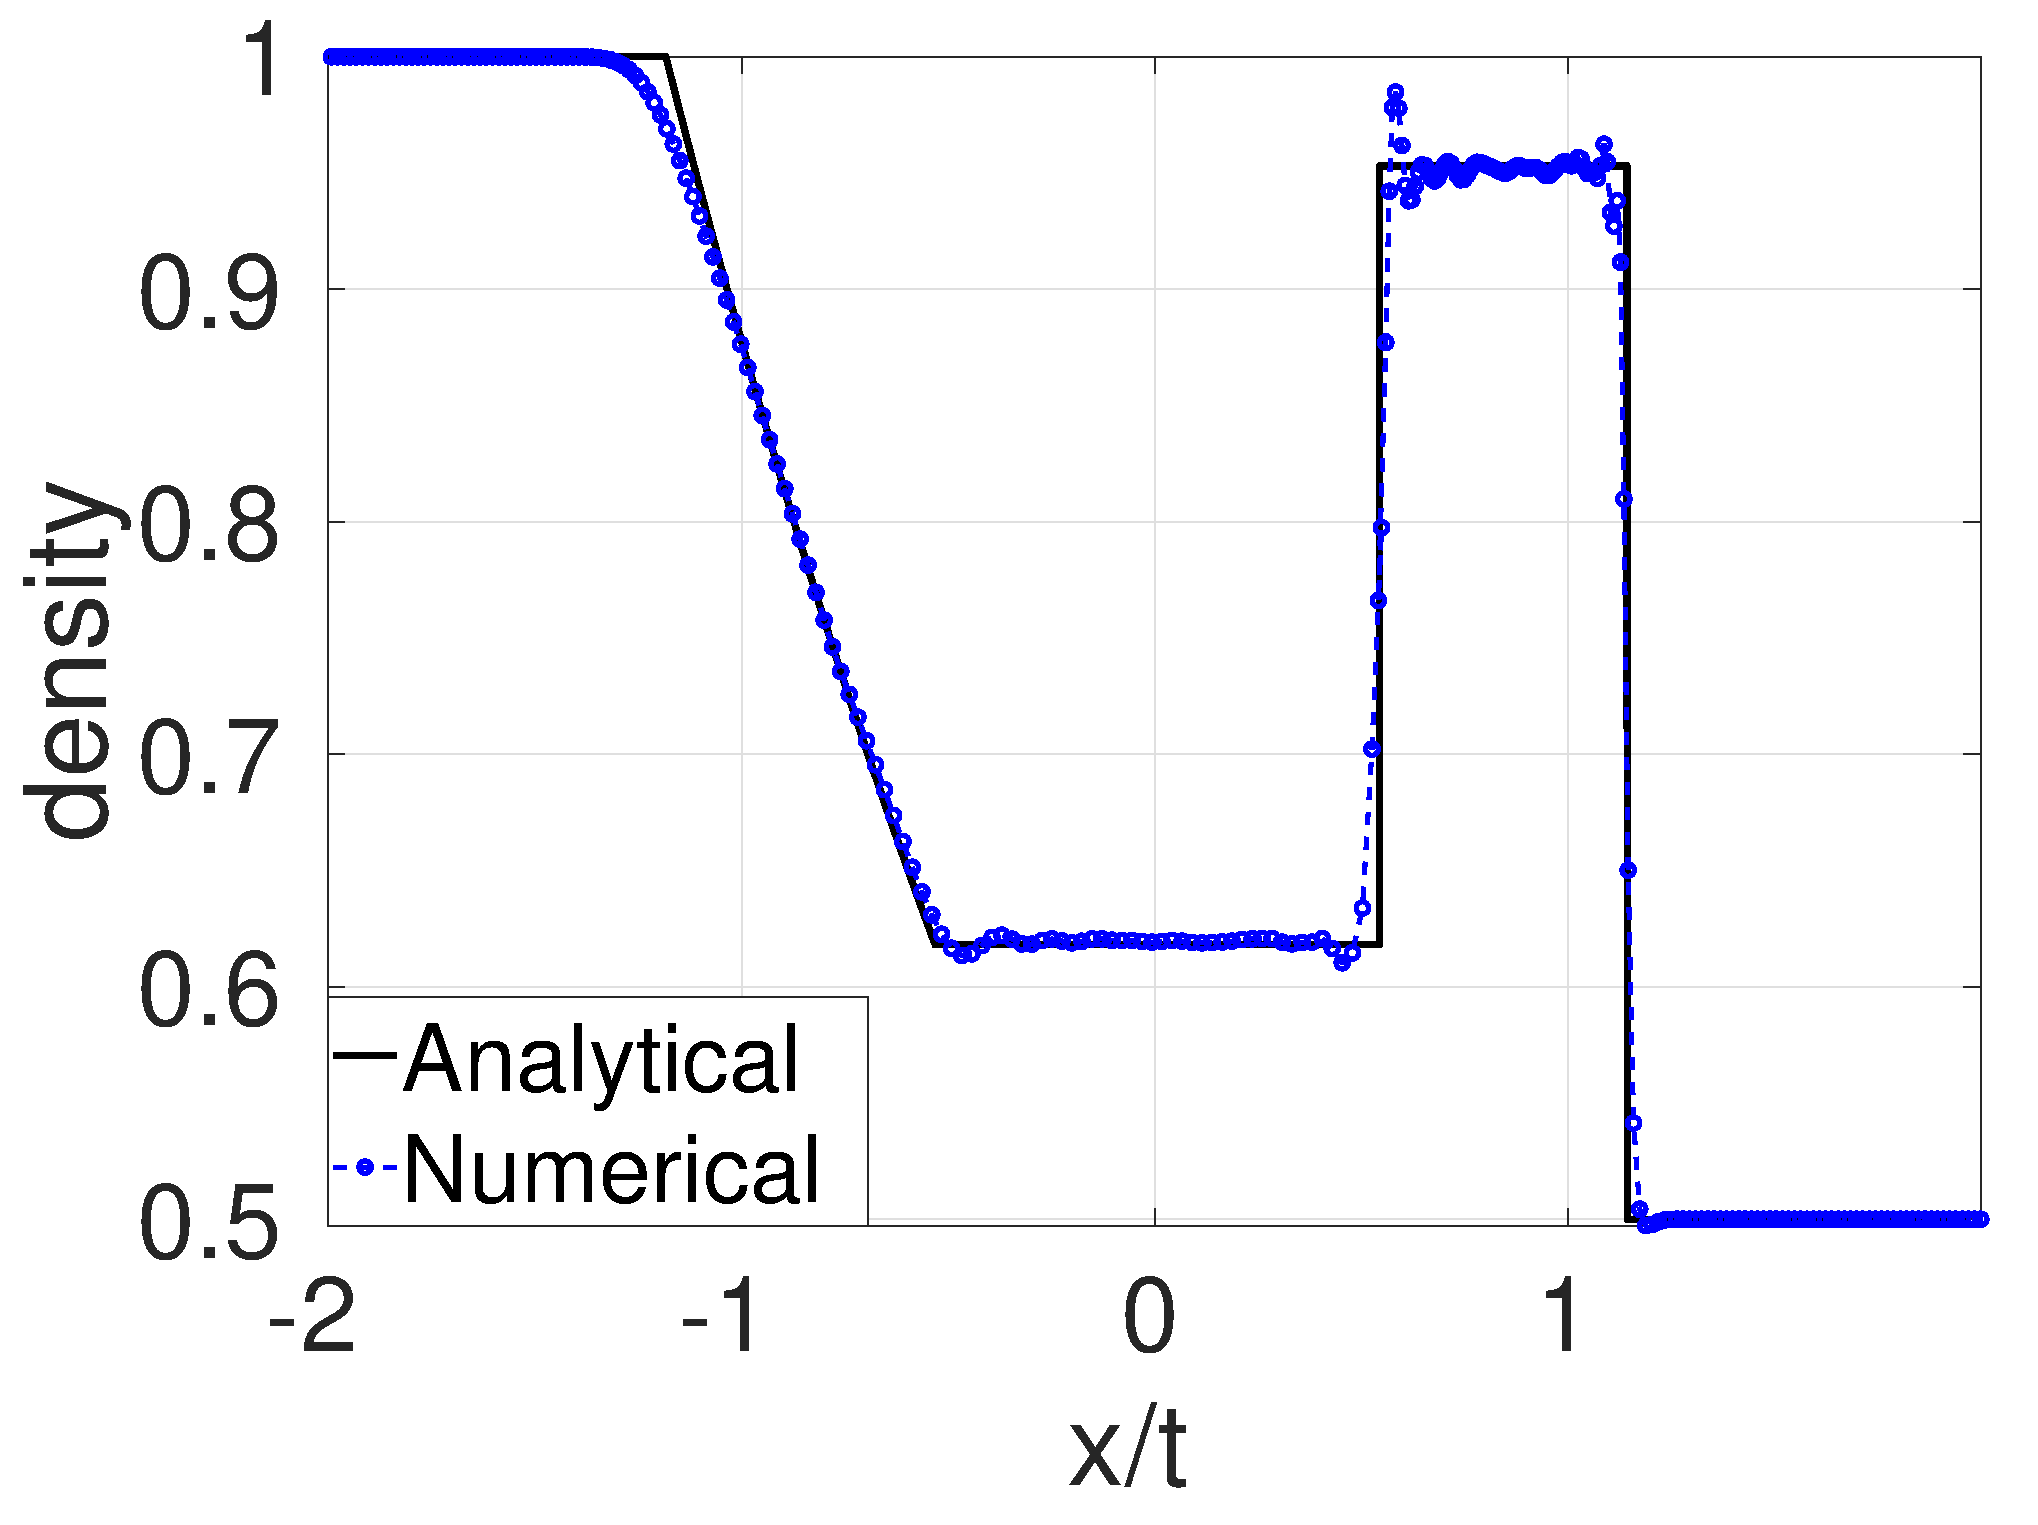
\includegraphics[width=0.99 \textwidth]{./Figures/GSPH-Sod/GRod-RCM-rho}
    \end{minipage}%
    \begin{minipage}{.495 \textwidth}
        \centering
        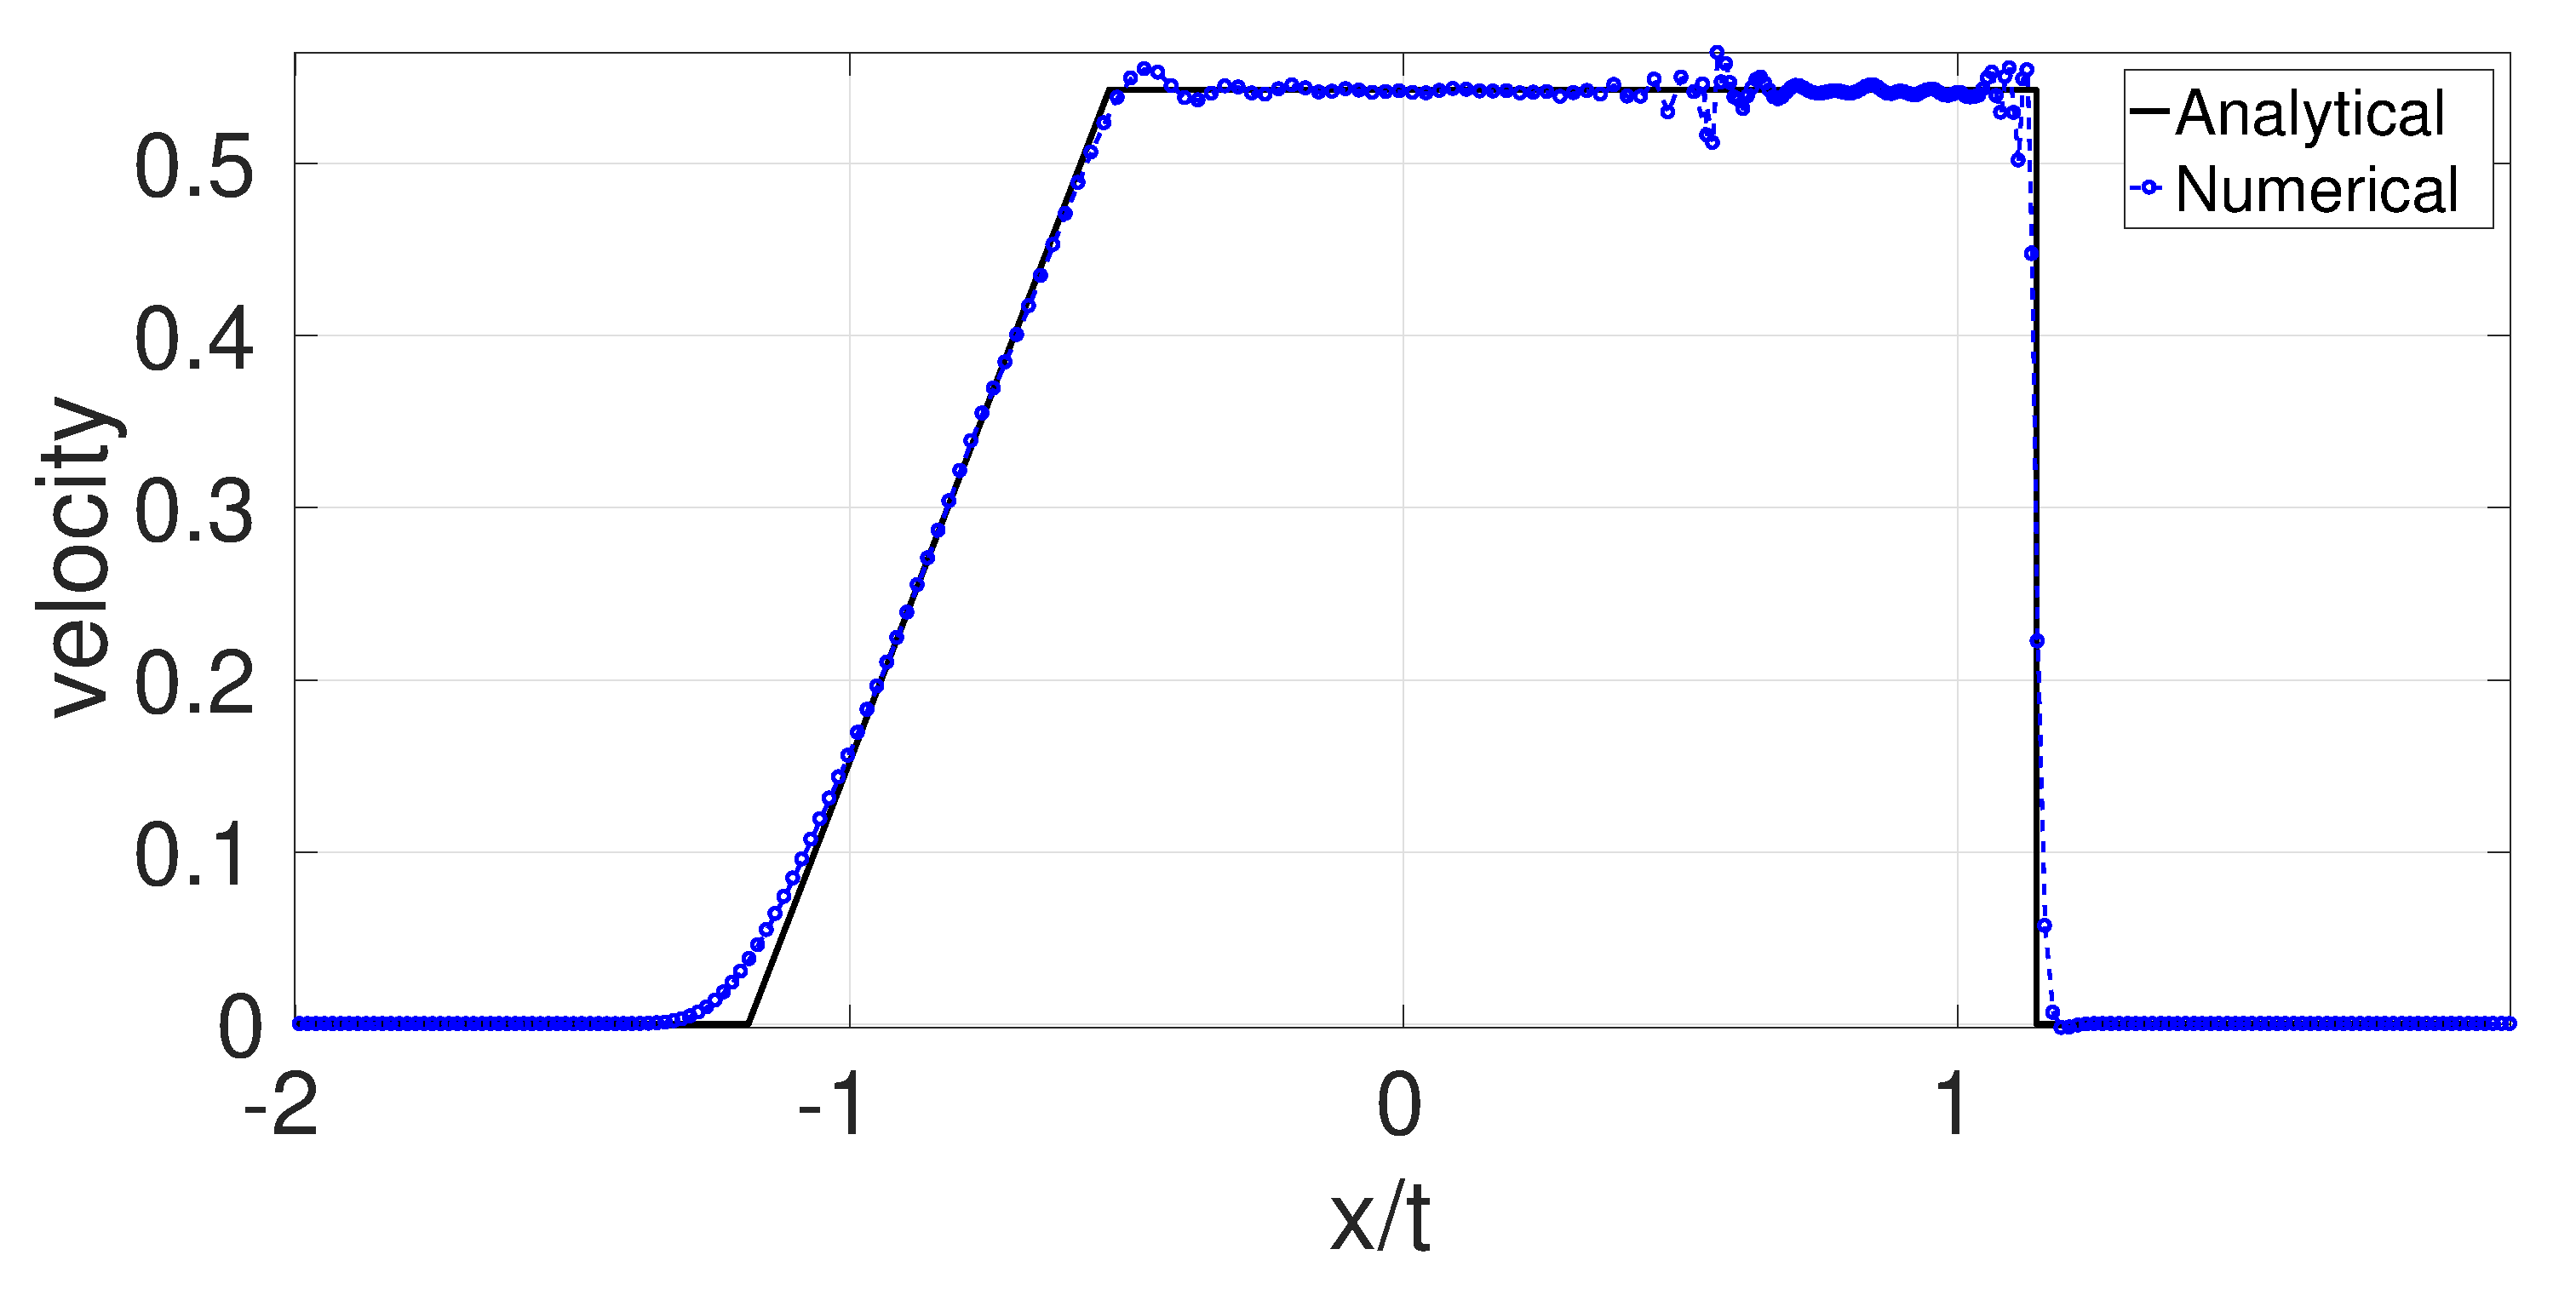
\includegraphics[width=0.99 \textwidth]{./Figures/GSPH-Sod/GRod-RCM-v}
    \end{minipage}% 
    \\
    \begin{minipage}{.495\textwidth}
        \centering
        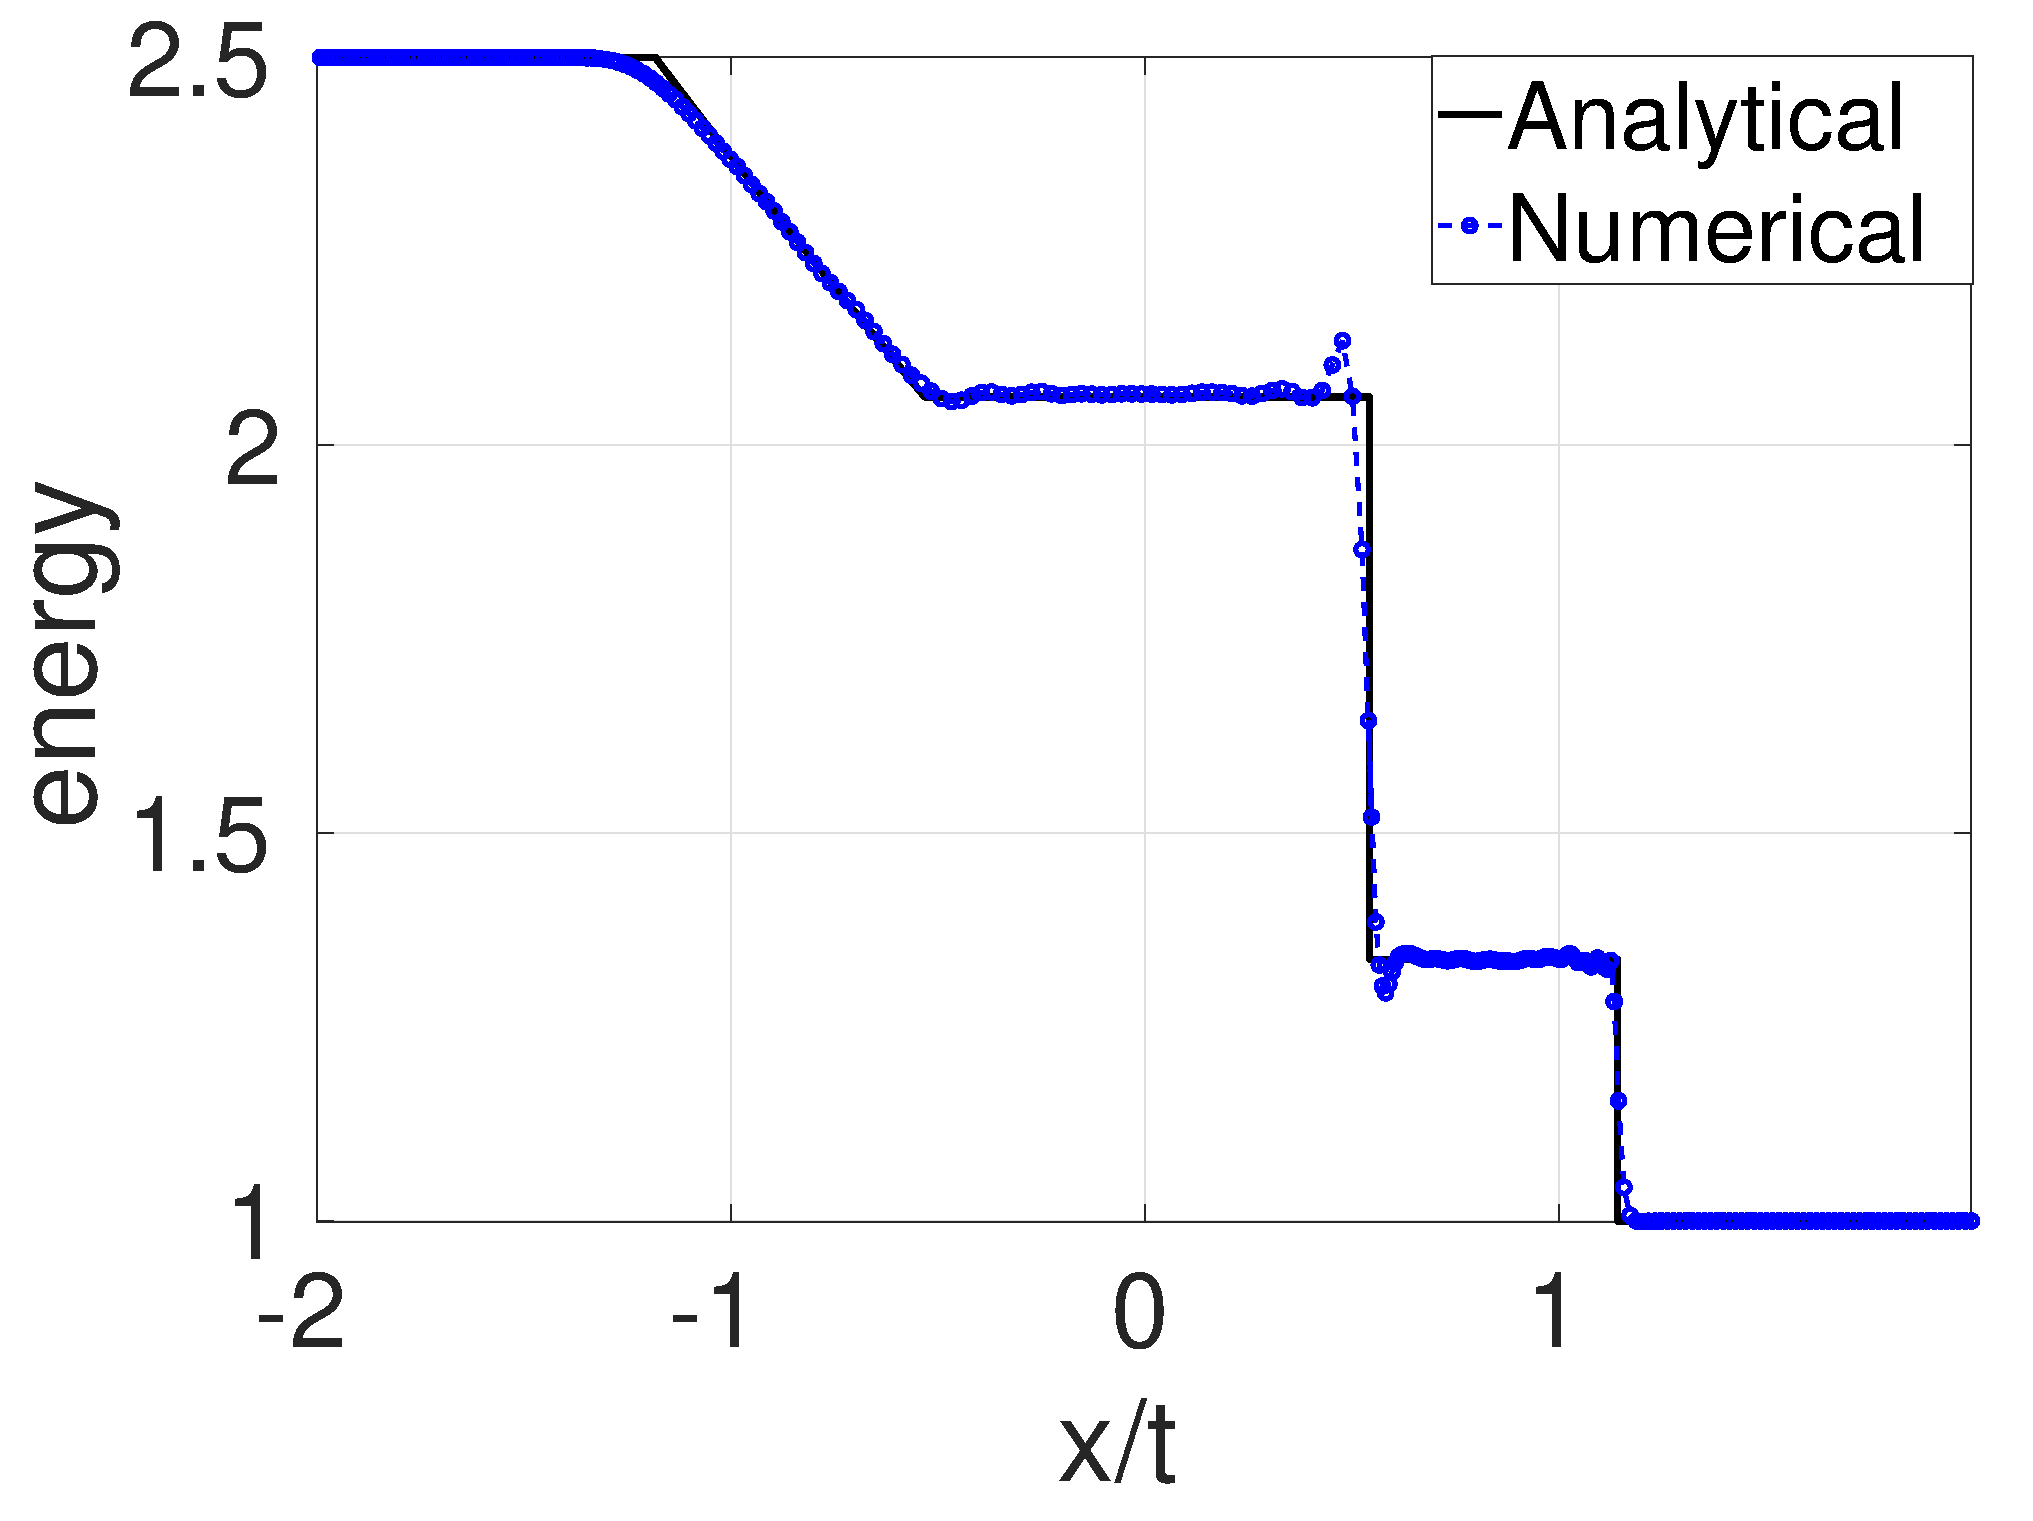
\includegraphics[width=0.99 \textwidth]{./Figures/GSPH-Sod/GRod-RCM-e}
    \end{minipage}%
    \begin{minipage}{.495 \textwidth}
        \centering
        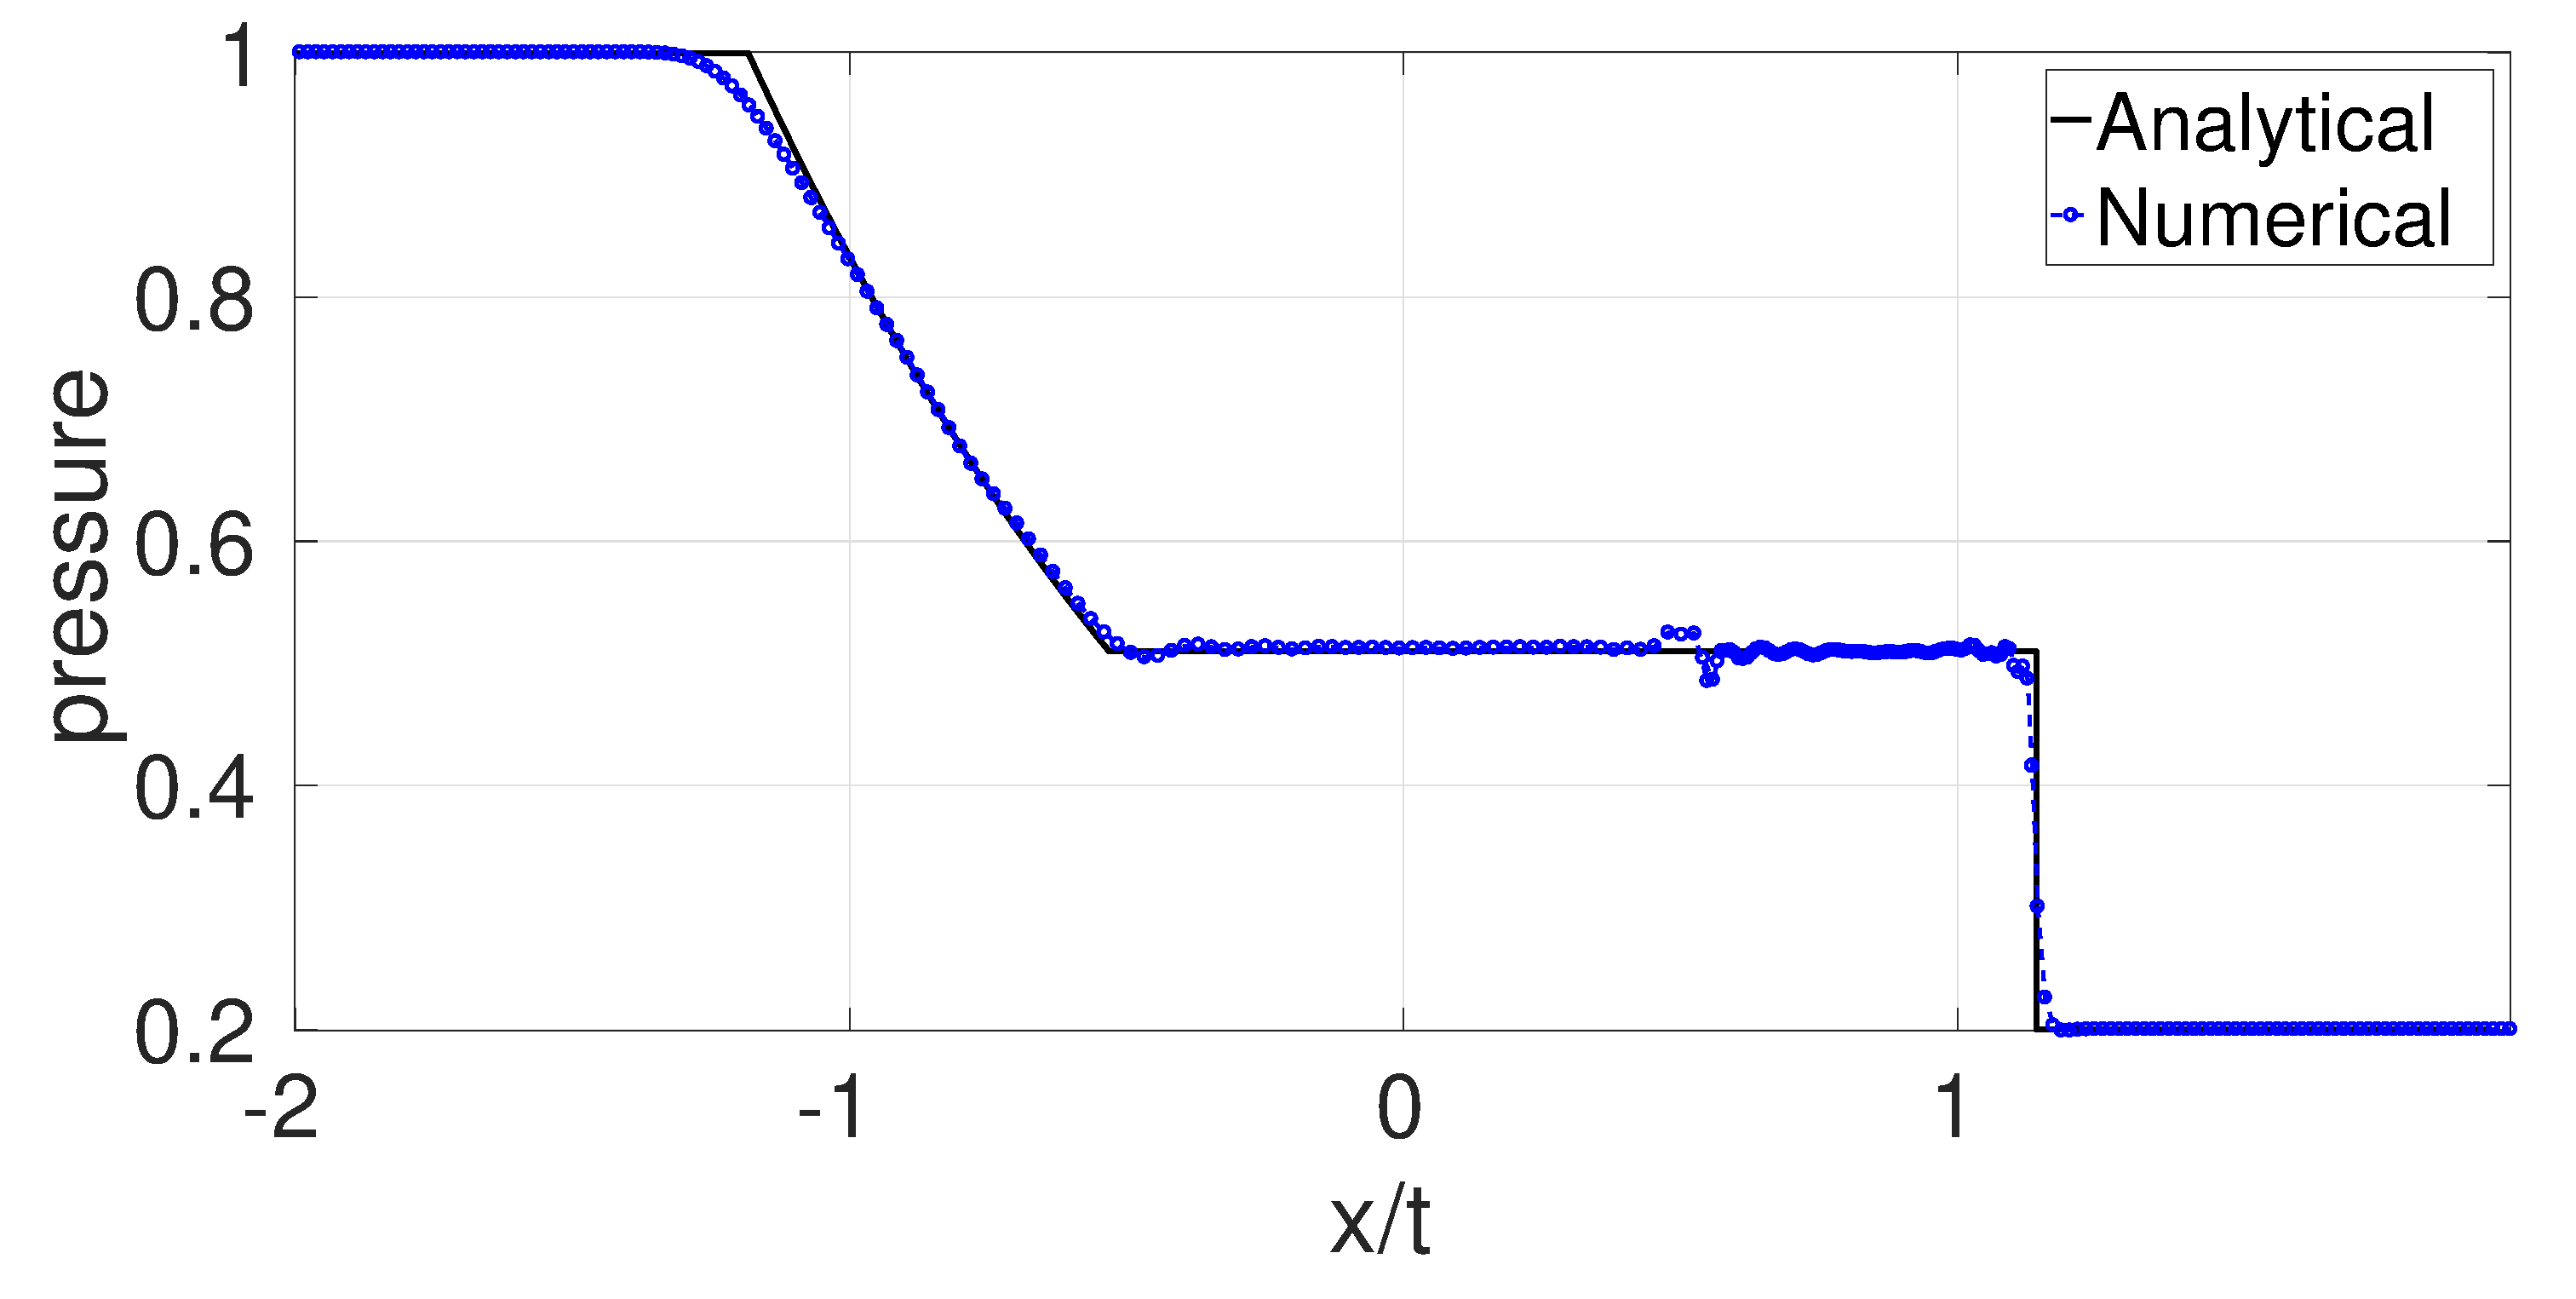
\includegraphics[width=0.99 \textwidth]{./Figures/GSPH-Sod/GRod-RCM-p}
    \end{minipage}% 
    \caption{Results for test 2, a variation of Sod test. All physical properties are well re-produced except for some acceptable oscillations}
    \label{fig:RCM-GSPH-Sod}
\end{figure}

\begin{figure}[H]
    \centering
    \begin{minipage}{.495\textwidth}
        \centering
        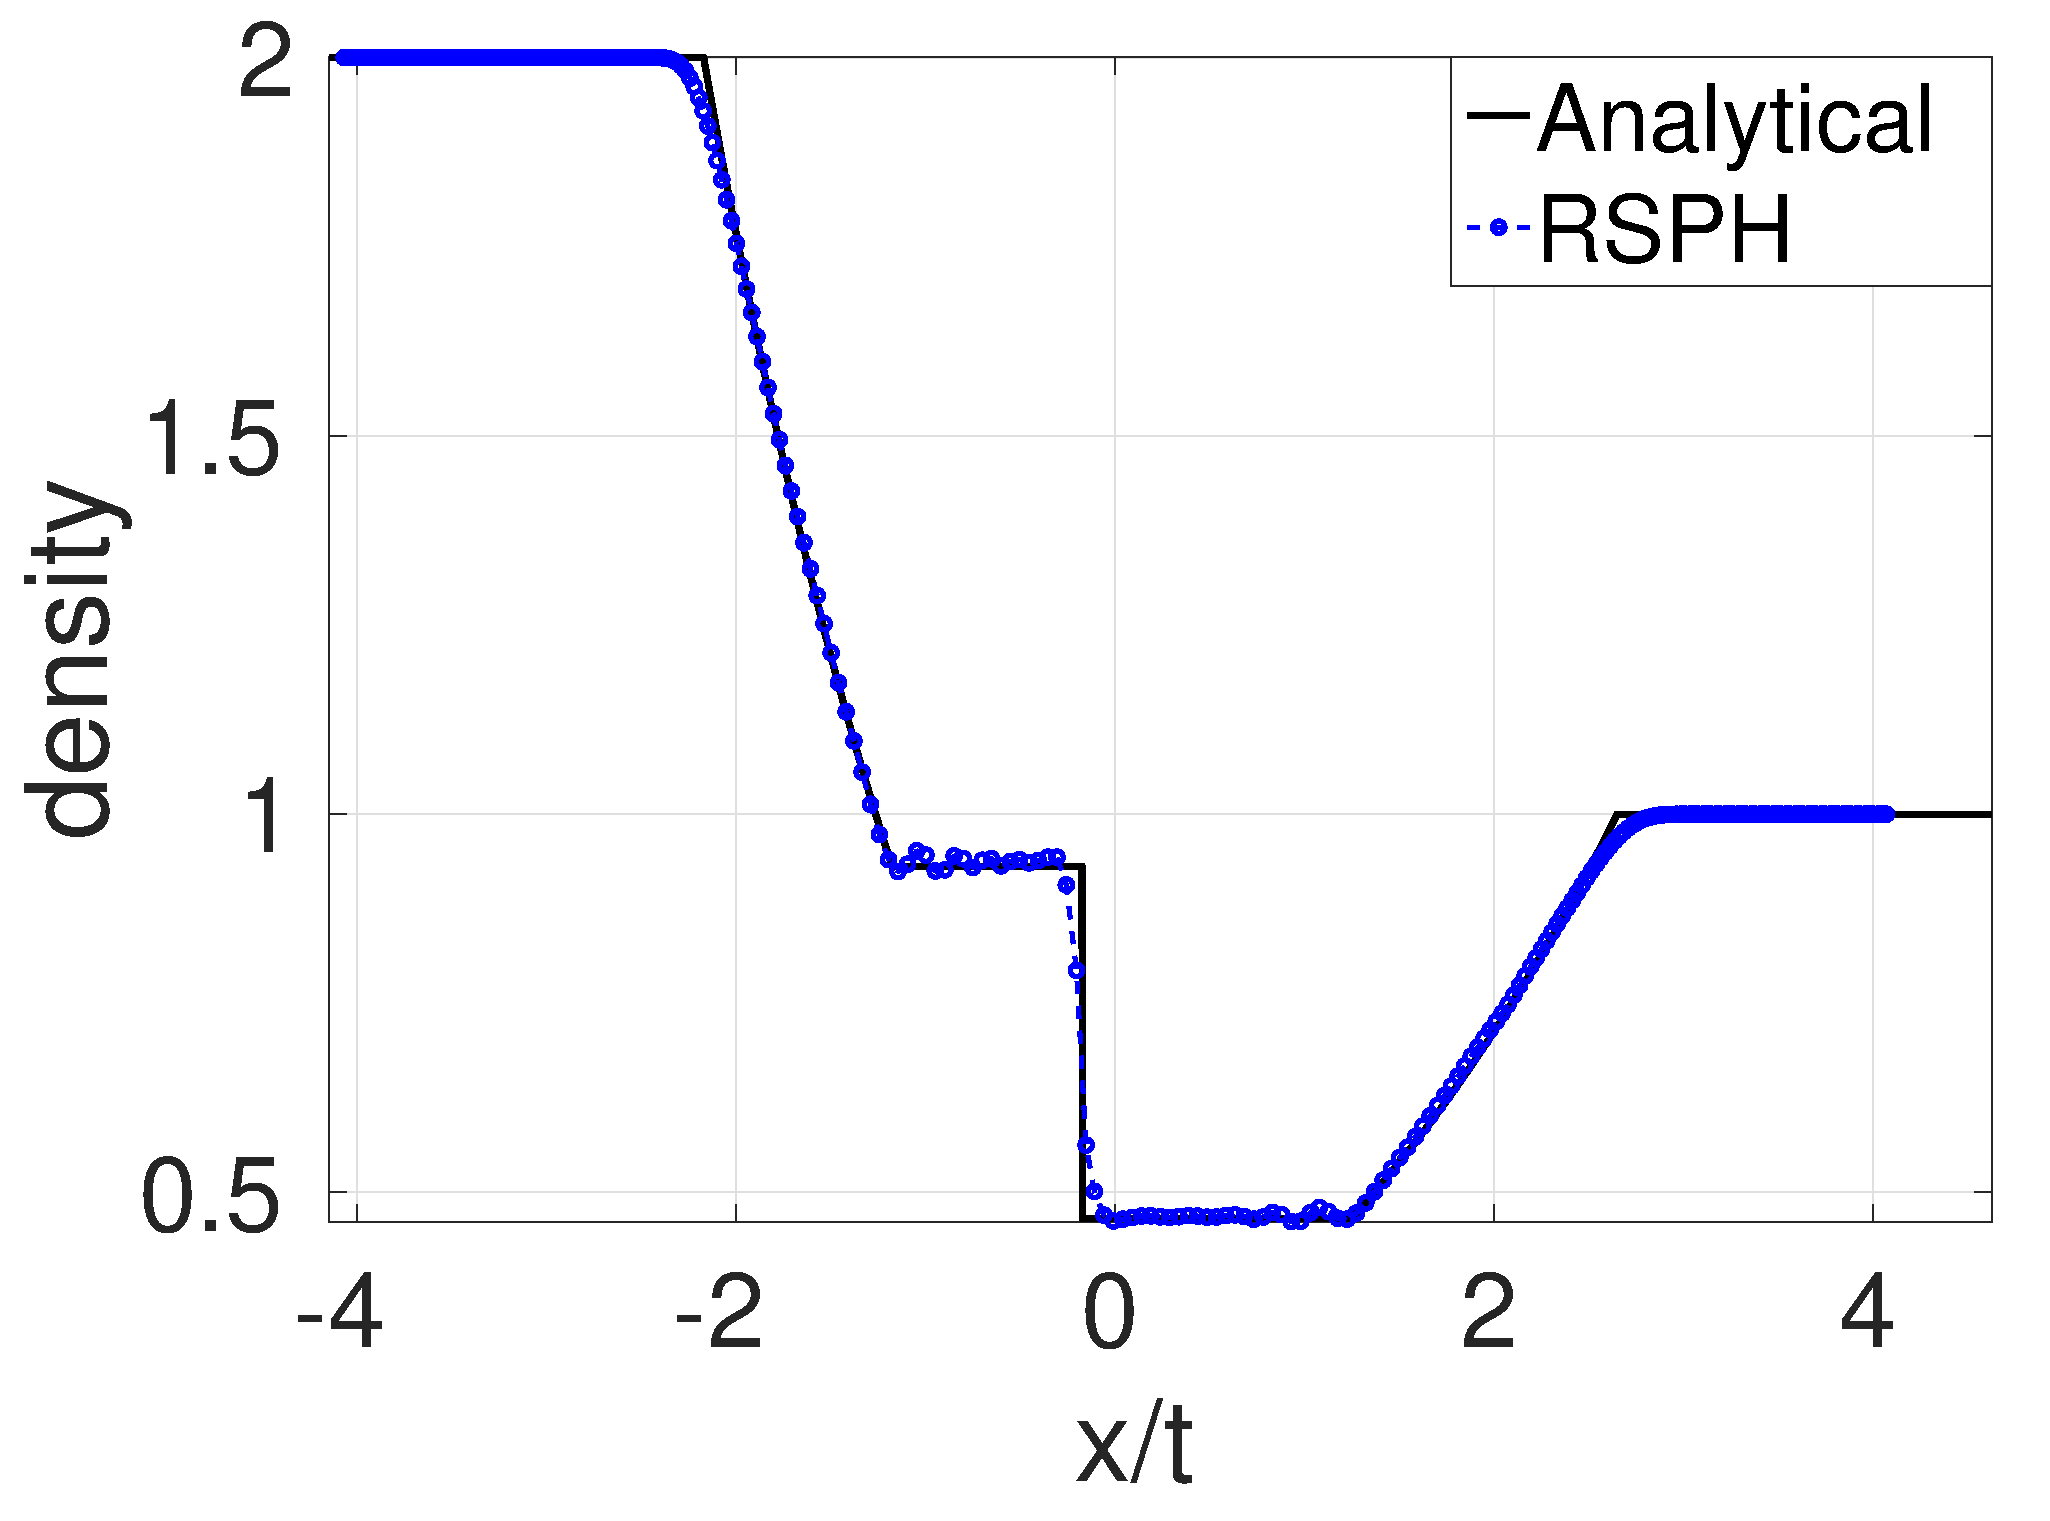
\includegraphics[width=0.99 \textwidth]{./Figures/double_exp/Dexp-RCM-rho}
    \end{minipage}%
    \begin{minipage}{.495 \textwidth}
        \centering
        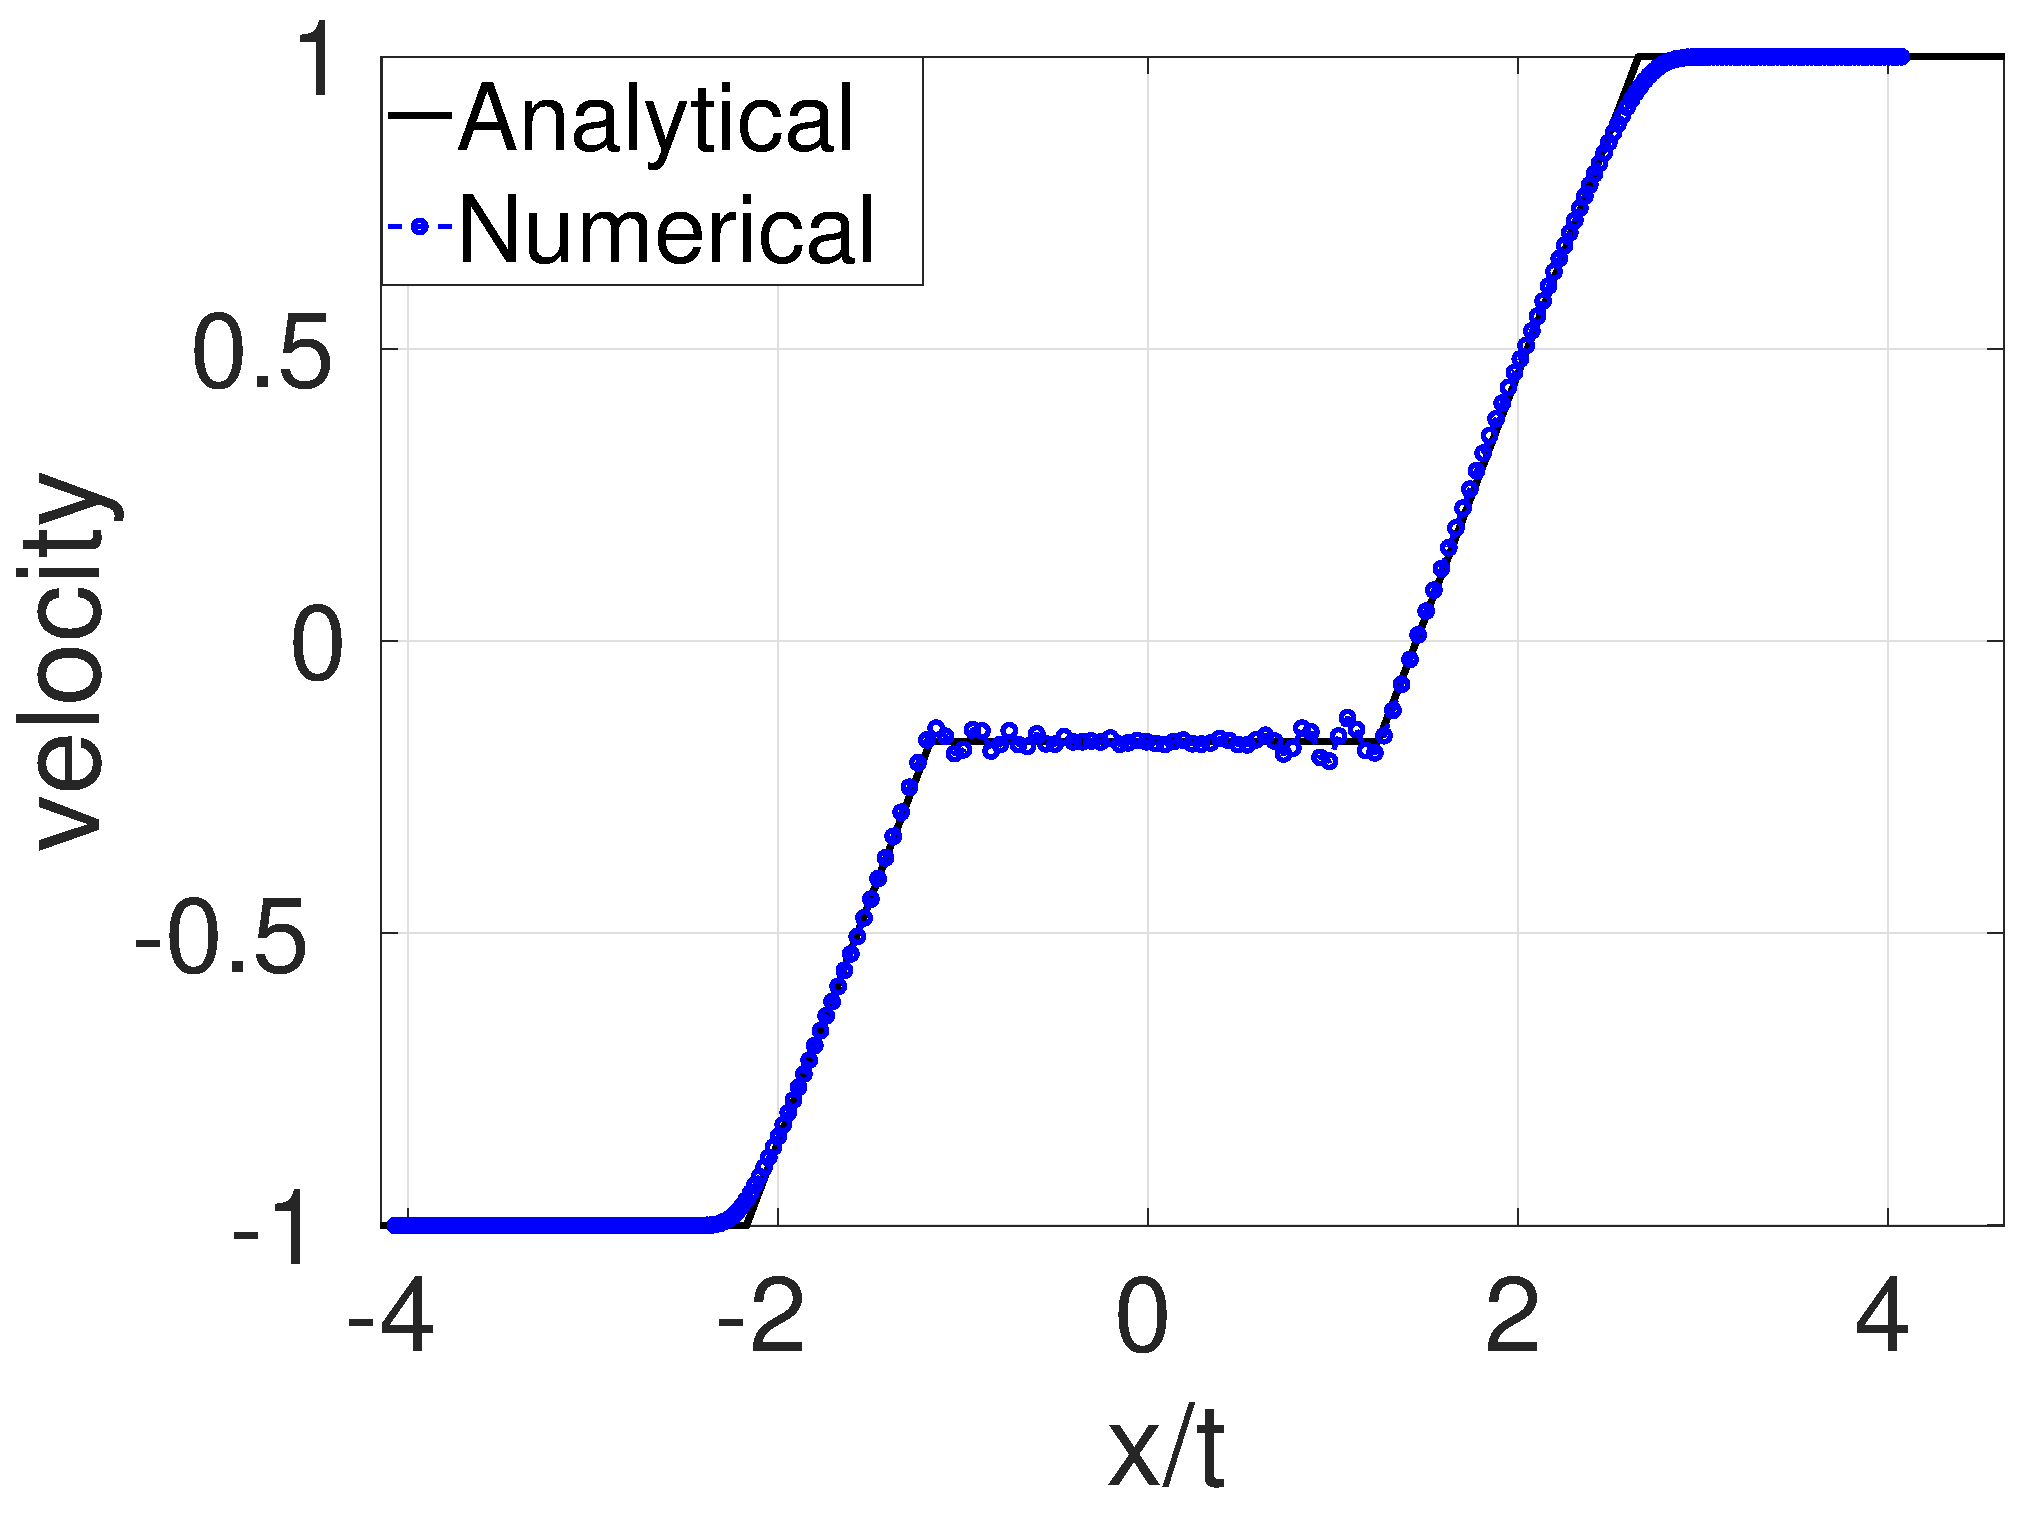
\includegraphics[width=0.99 \textwidth]{./Figures/double_exp/Dexp-RCM-v}
    \end{minipage}%
    \\
    \begin{minipage}{.495\textwidth}
        \centering
        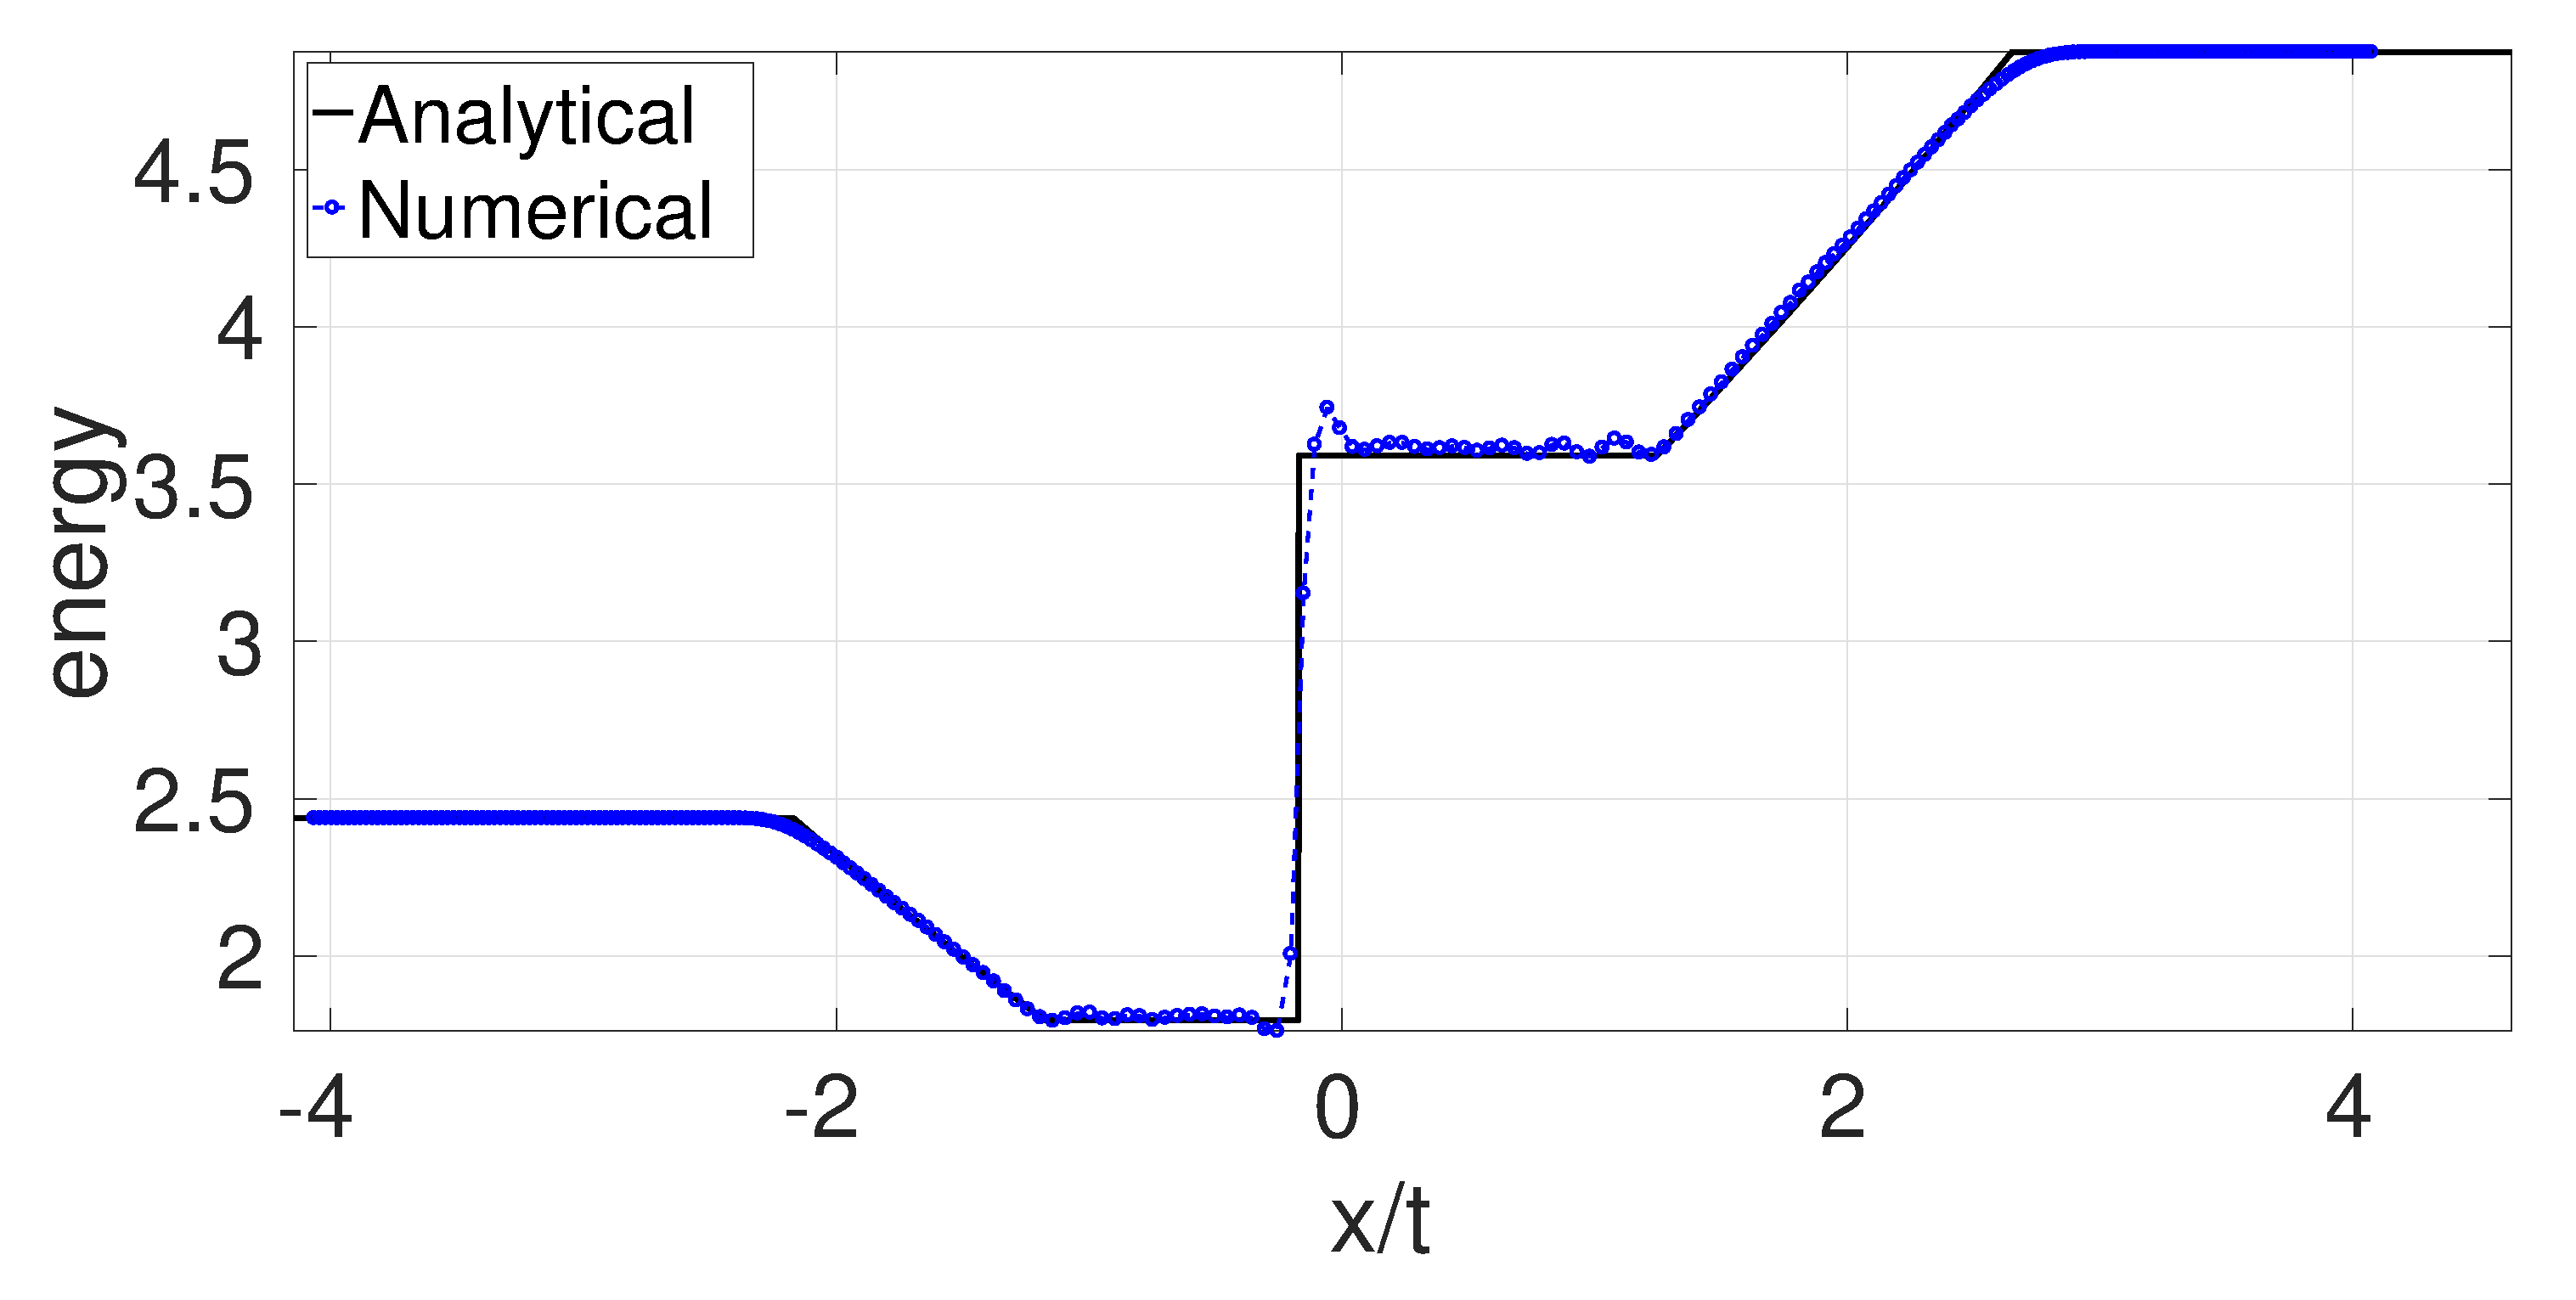
\includegraphics[width=0.99 \textwidth]{./Figures/double_exp/Dexp-RCM-e}
    \end{minipage}%
    \begin{minipage}{.495 \textwidth}
        \centering
        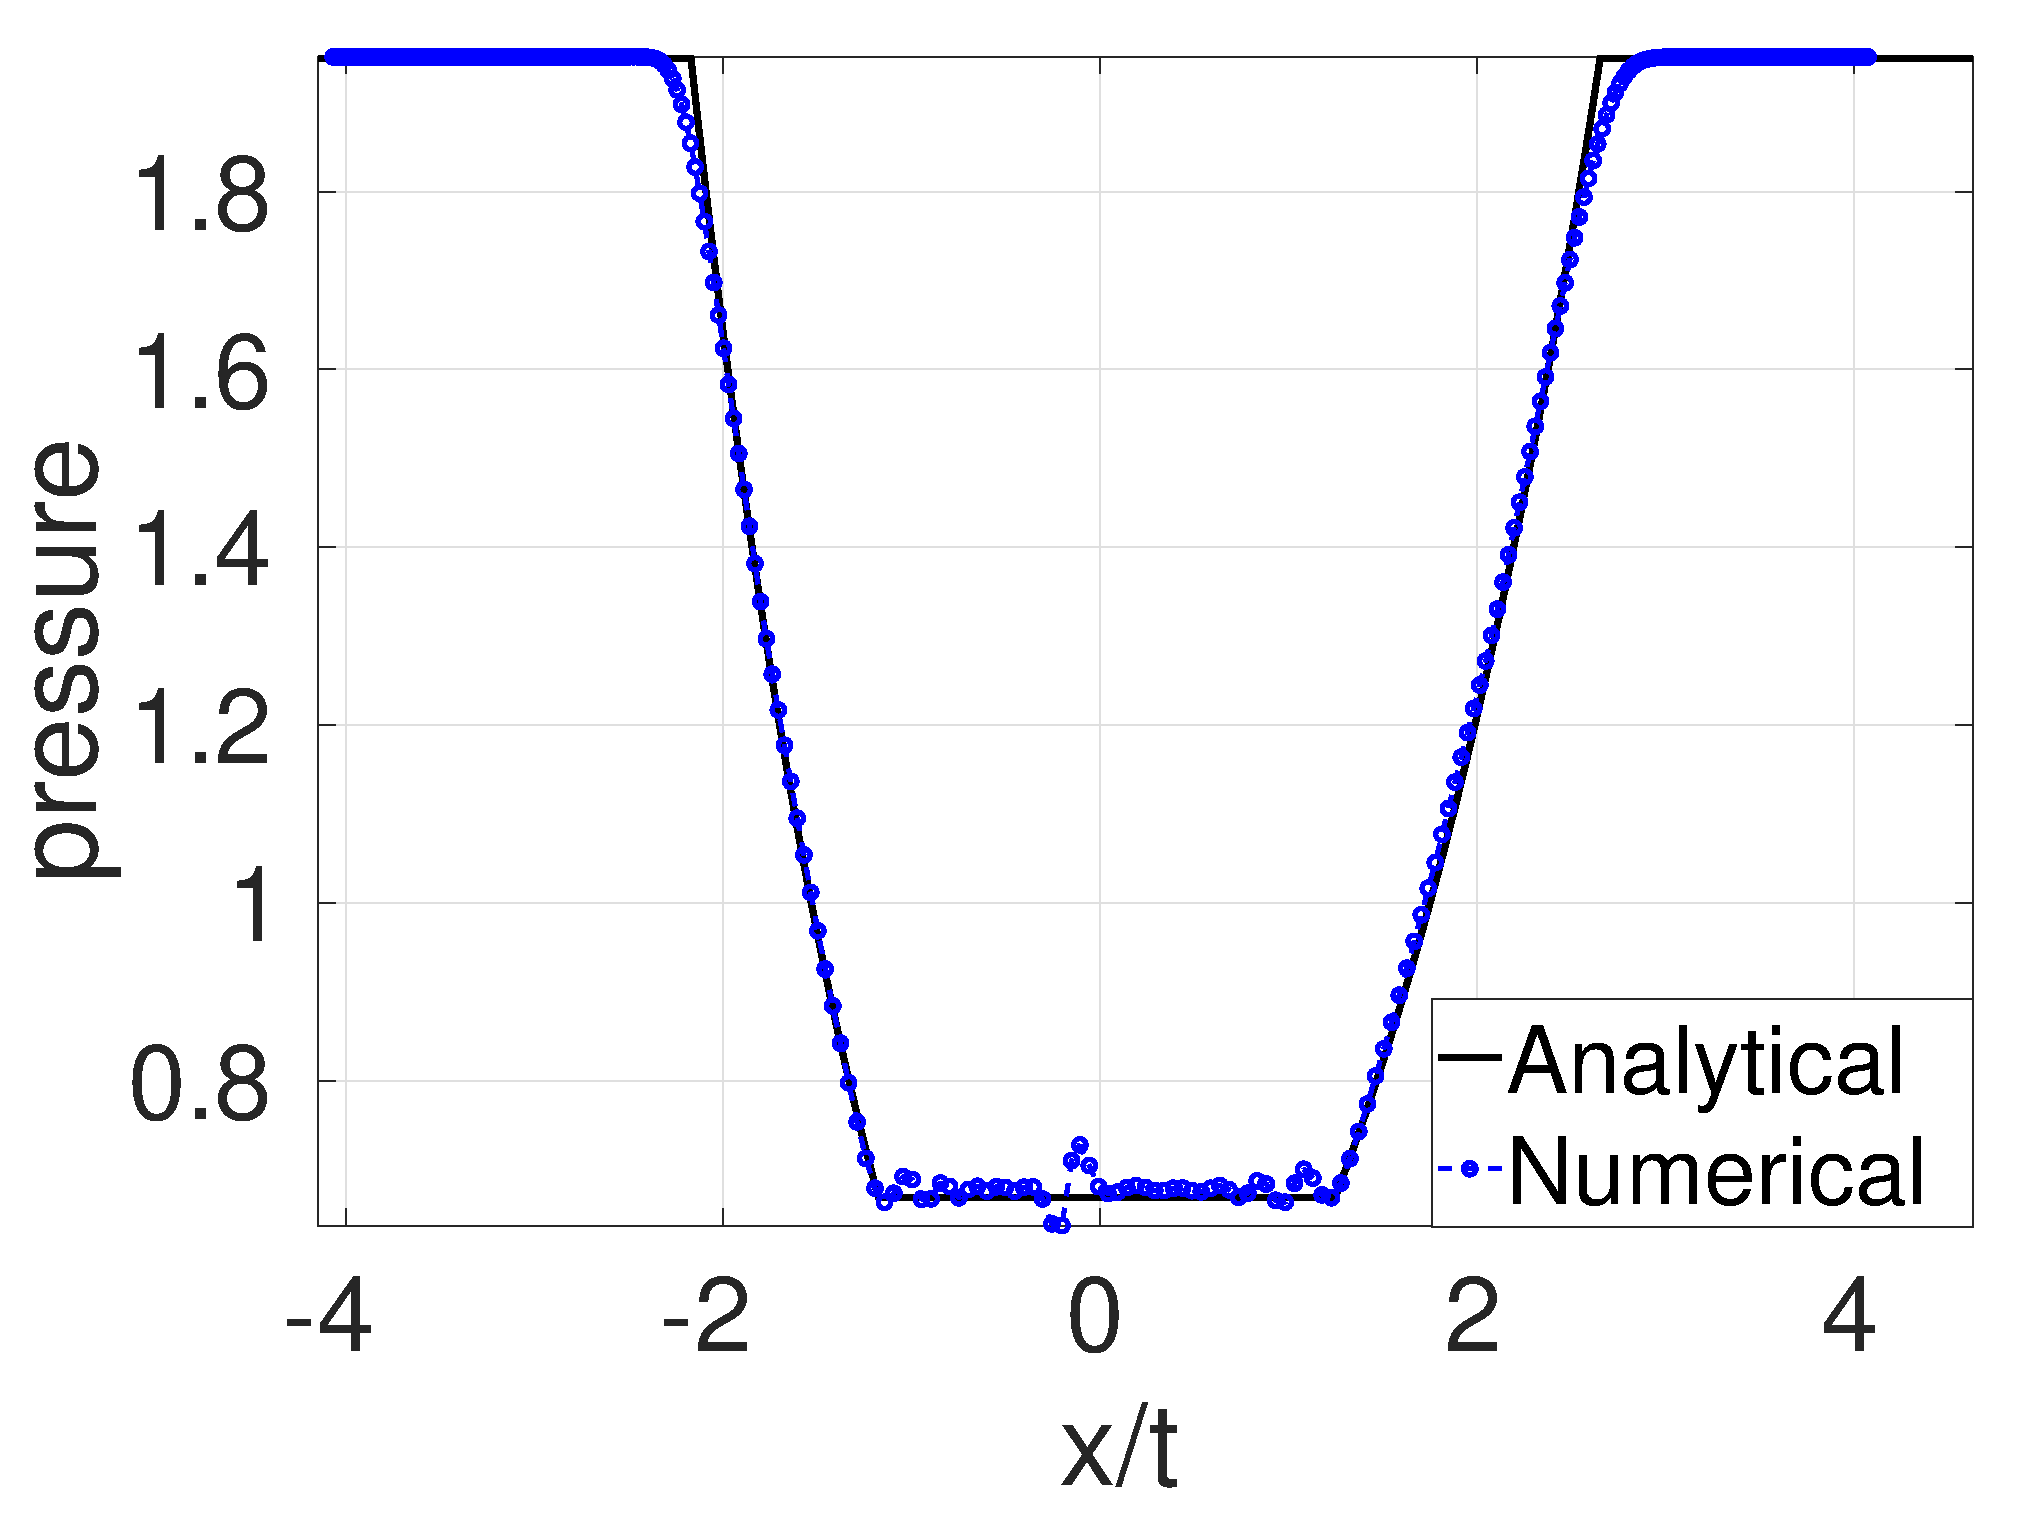
\includegraphics[width=0.99 \textwidth]{./Figures/double_exp/Dexp-RCM-p}
    \end{minipage}% 
    \caption{Results for test 3, the double expansion case. All physical properties are well re-produced except for some oscillations}
    \label{fig:RCM-double-expansion}
\end{figure}

\begin{figure}[H]
    %\centering
    \begin{minipage}{.495\textwidth}
        \centering
        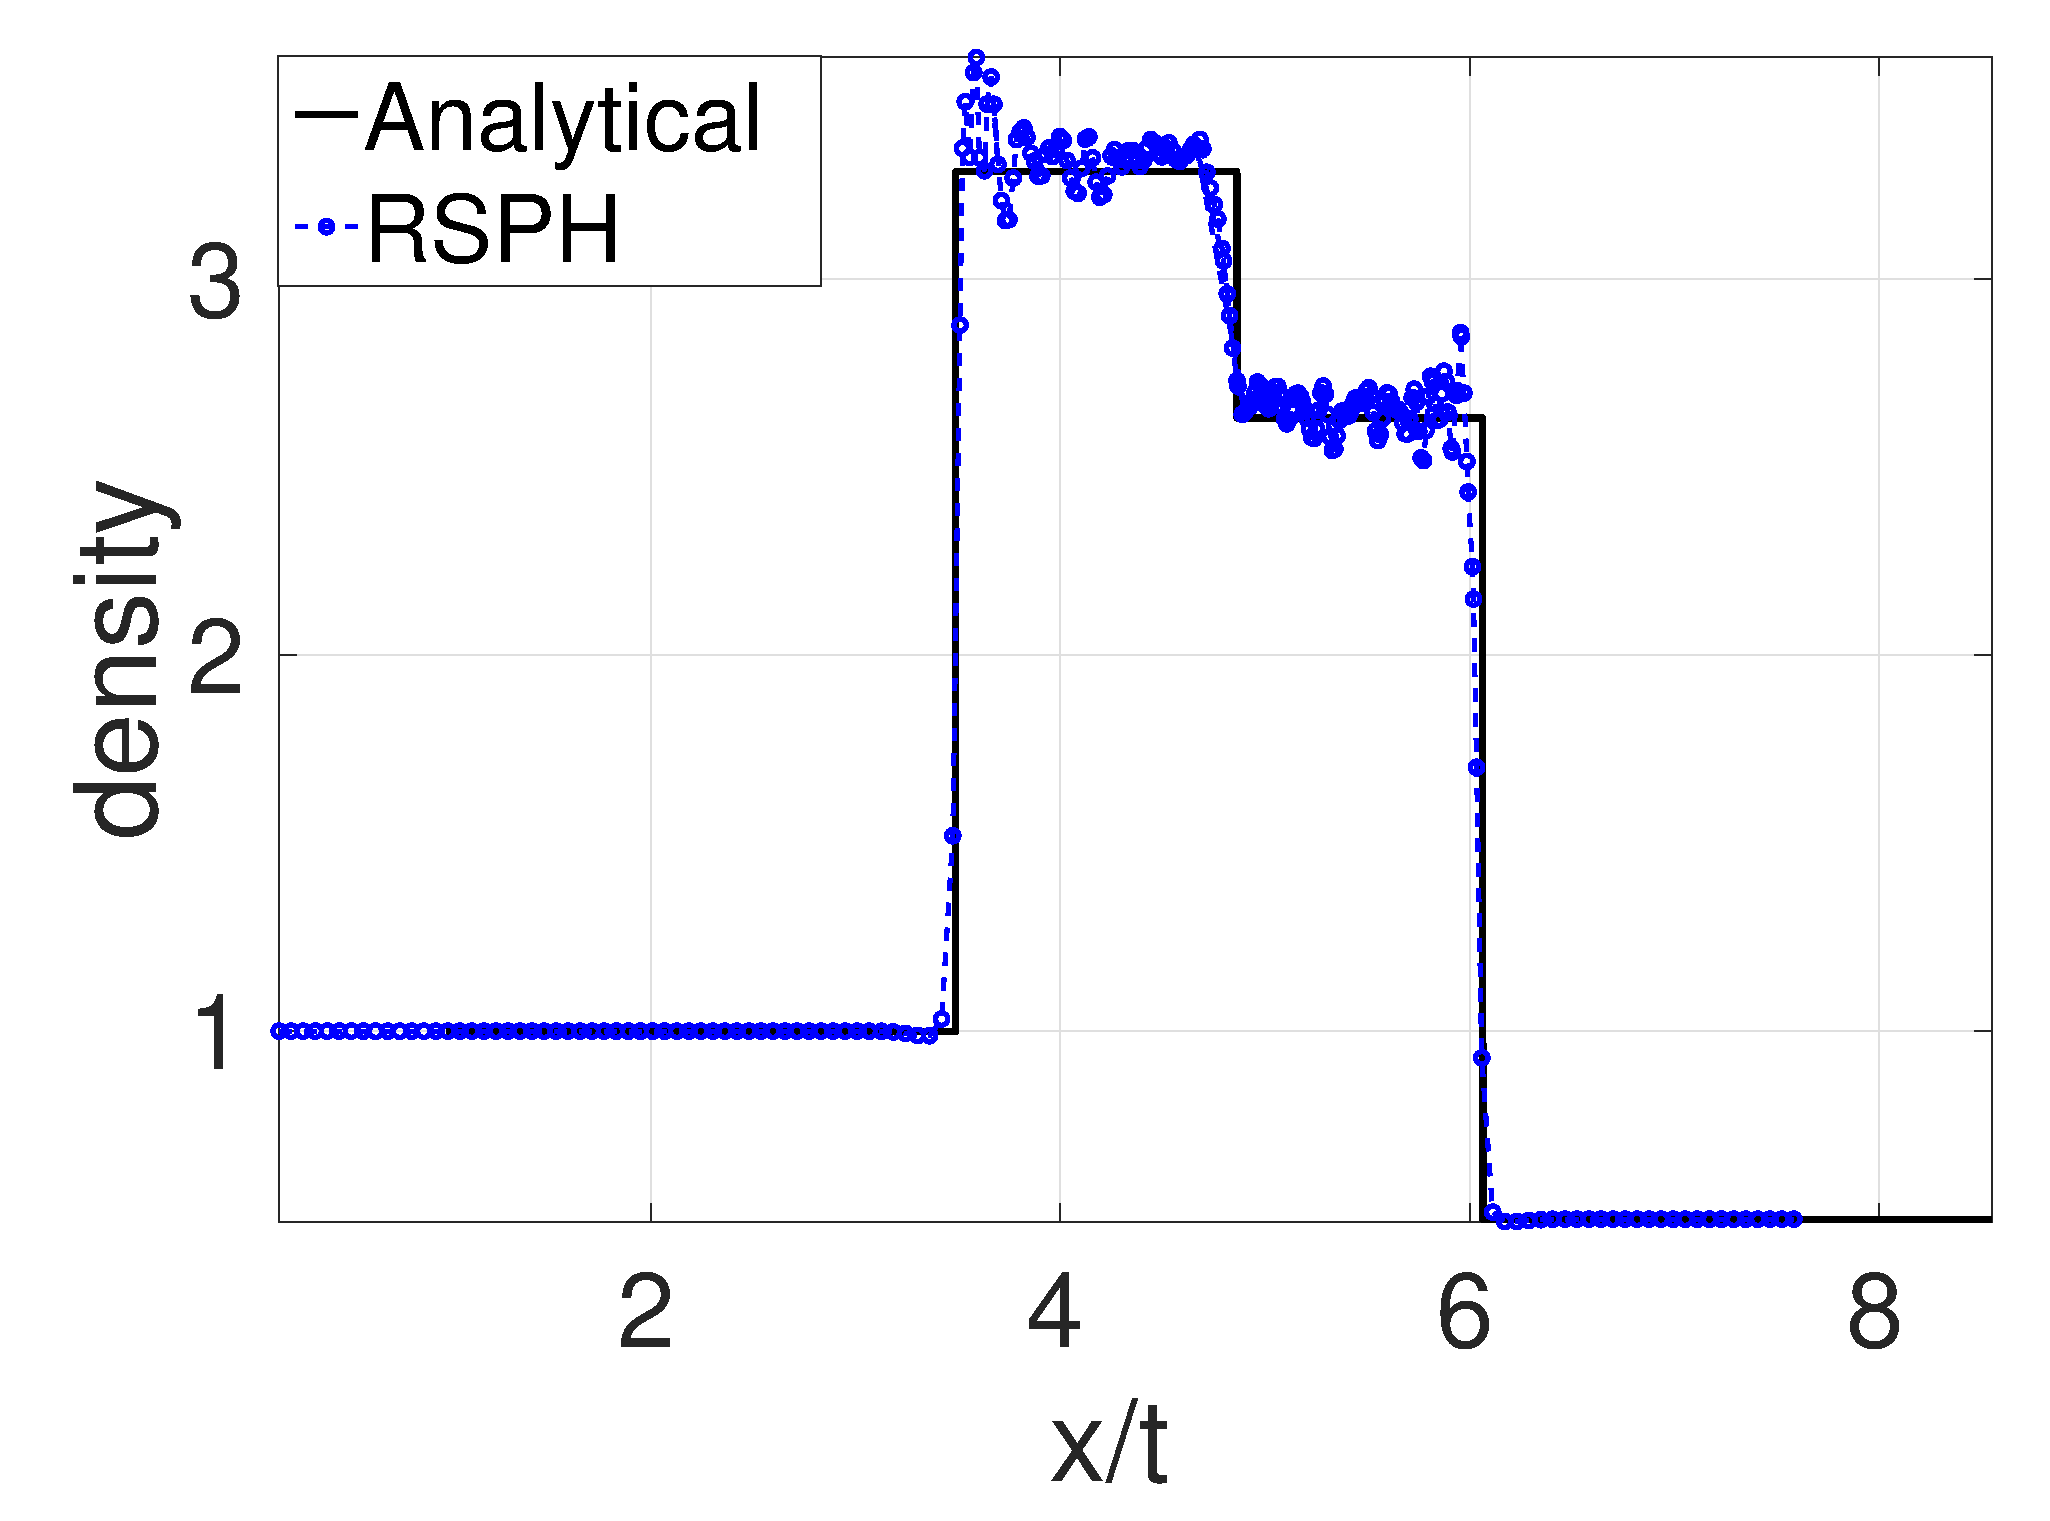
\includegraphics[width=0.99 \textwidth]{./Figures/double_shock/Dshock-RCM-rho-Rp6}
    \end{minipage}%
    \begin{minipage}{.495 \textwidth}
        \centering
        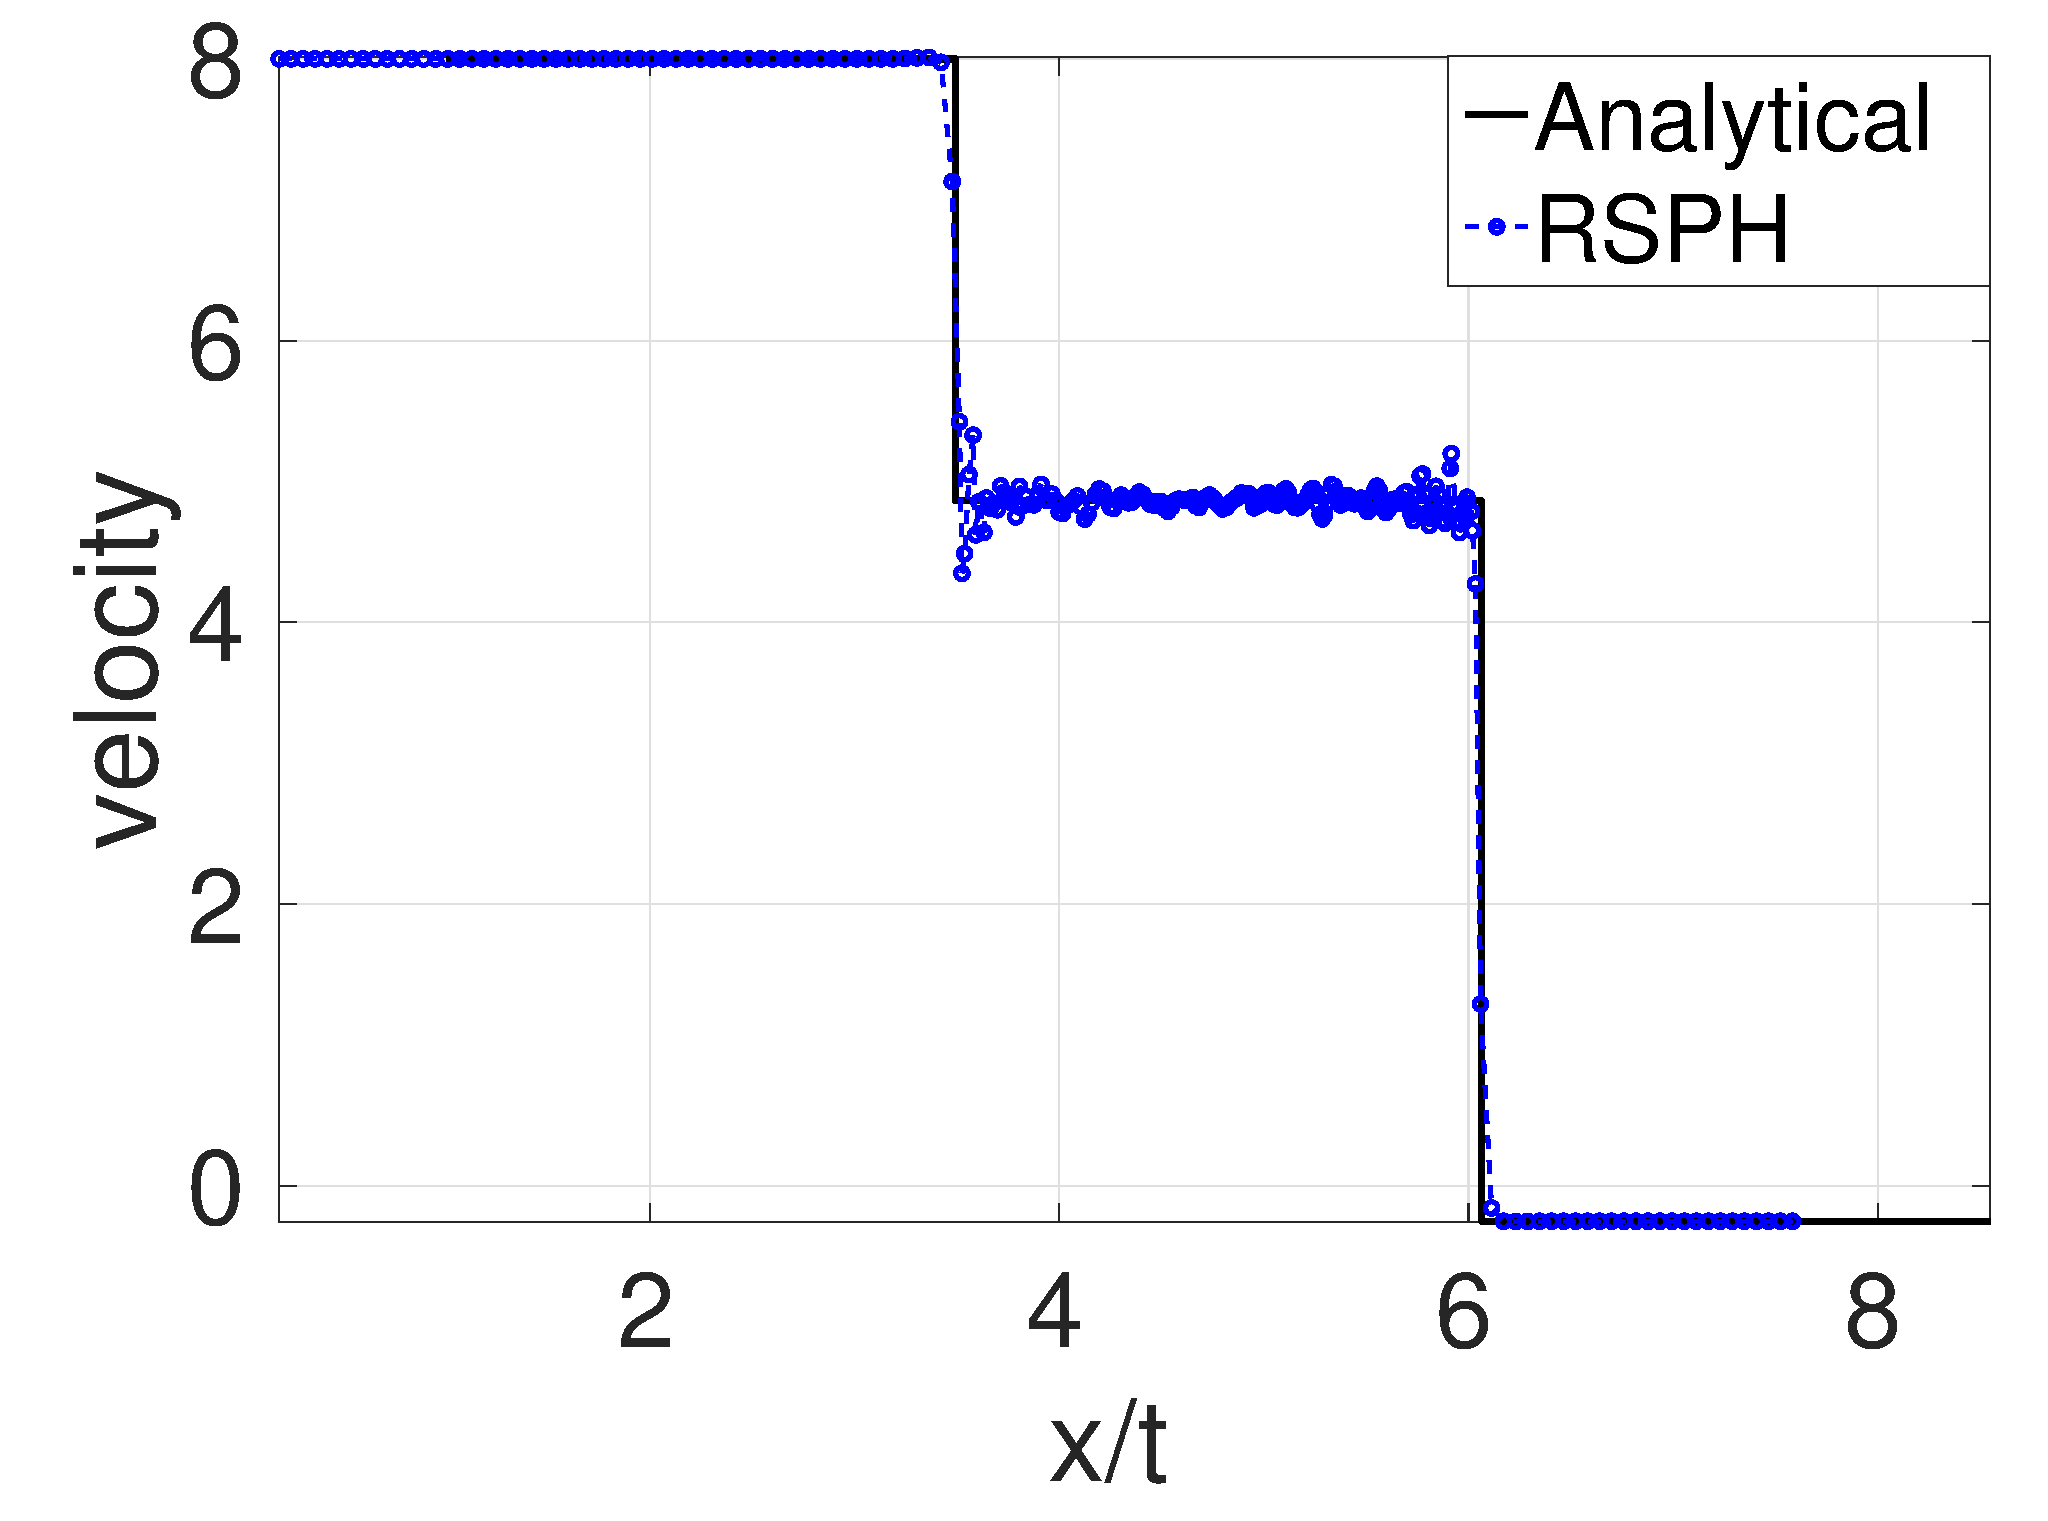
\includegraphics[width=0.99 \textwidth]{./Figures/double_shock/Dshock-RCM-v-Rp6}
    \end{minipage}%
    \\
    \begin{minipage}{.495\textwidth}
        \centering
        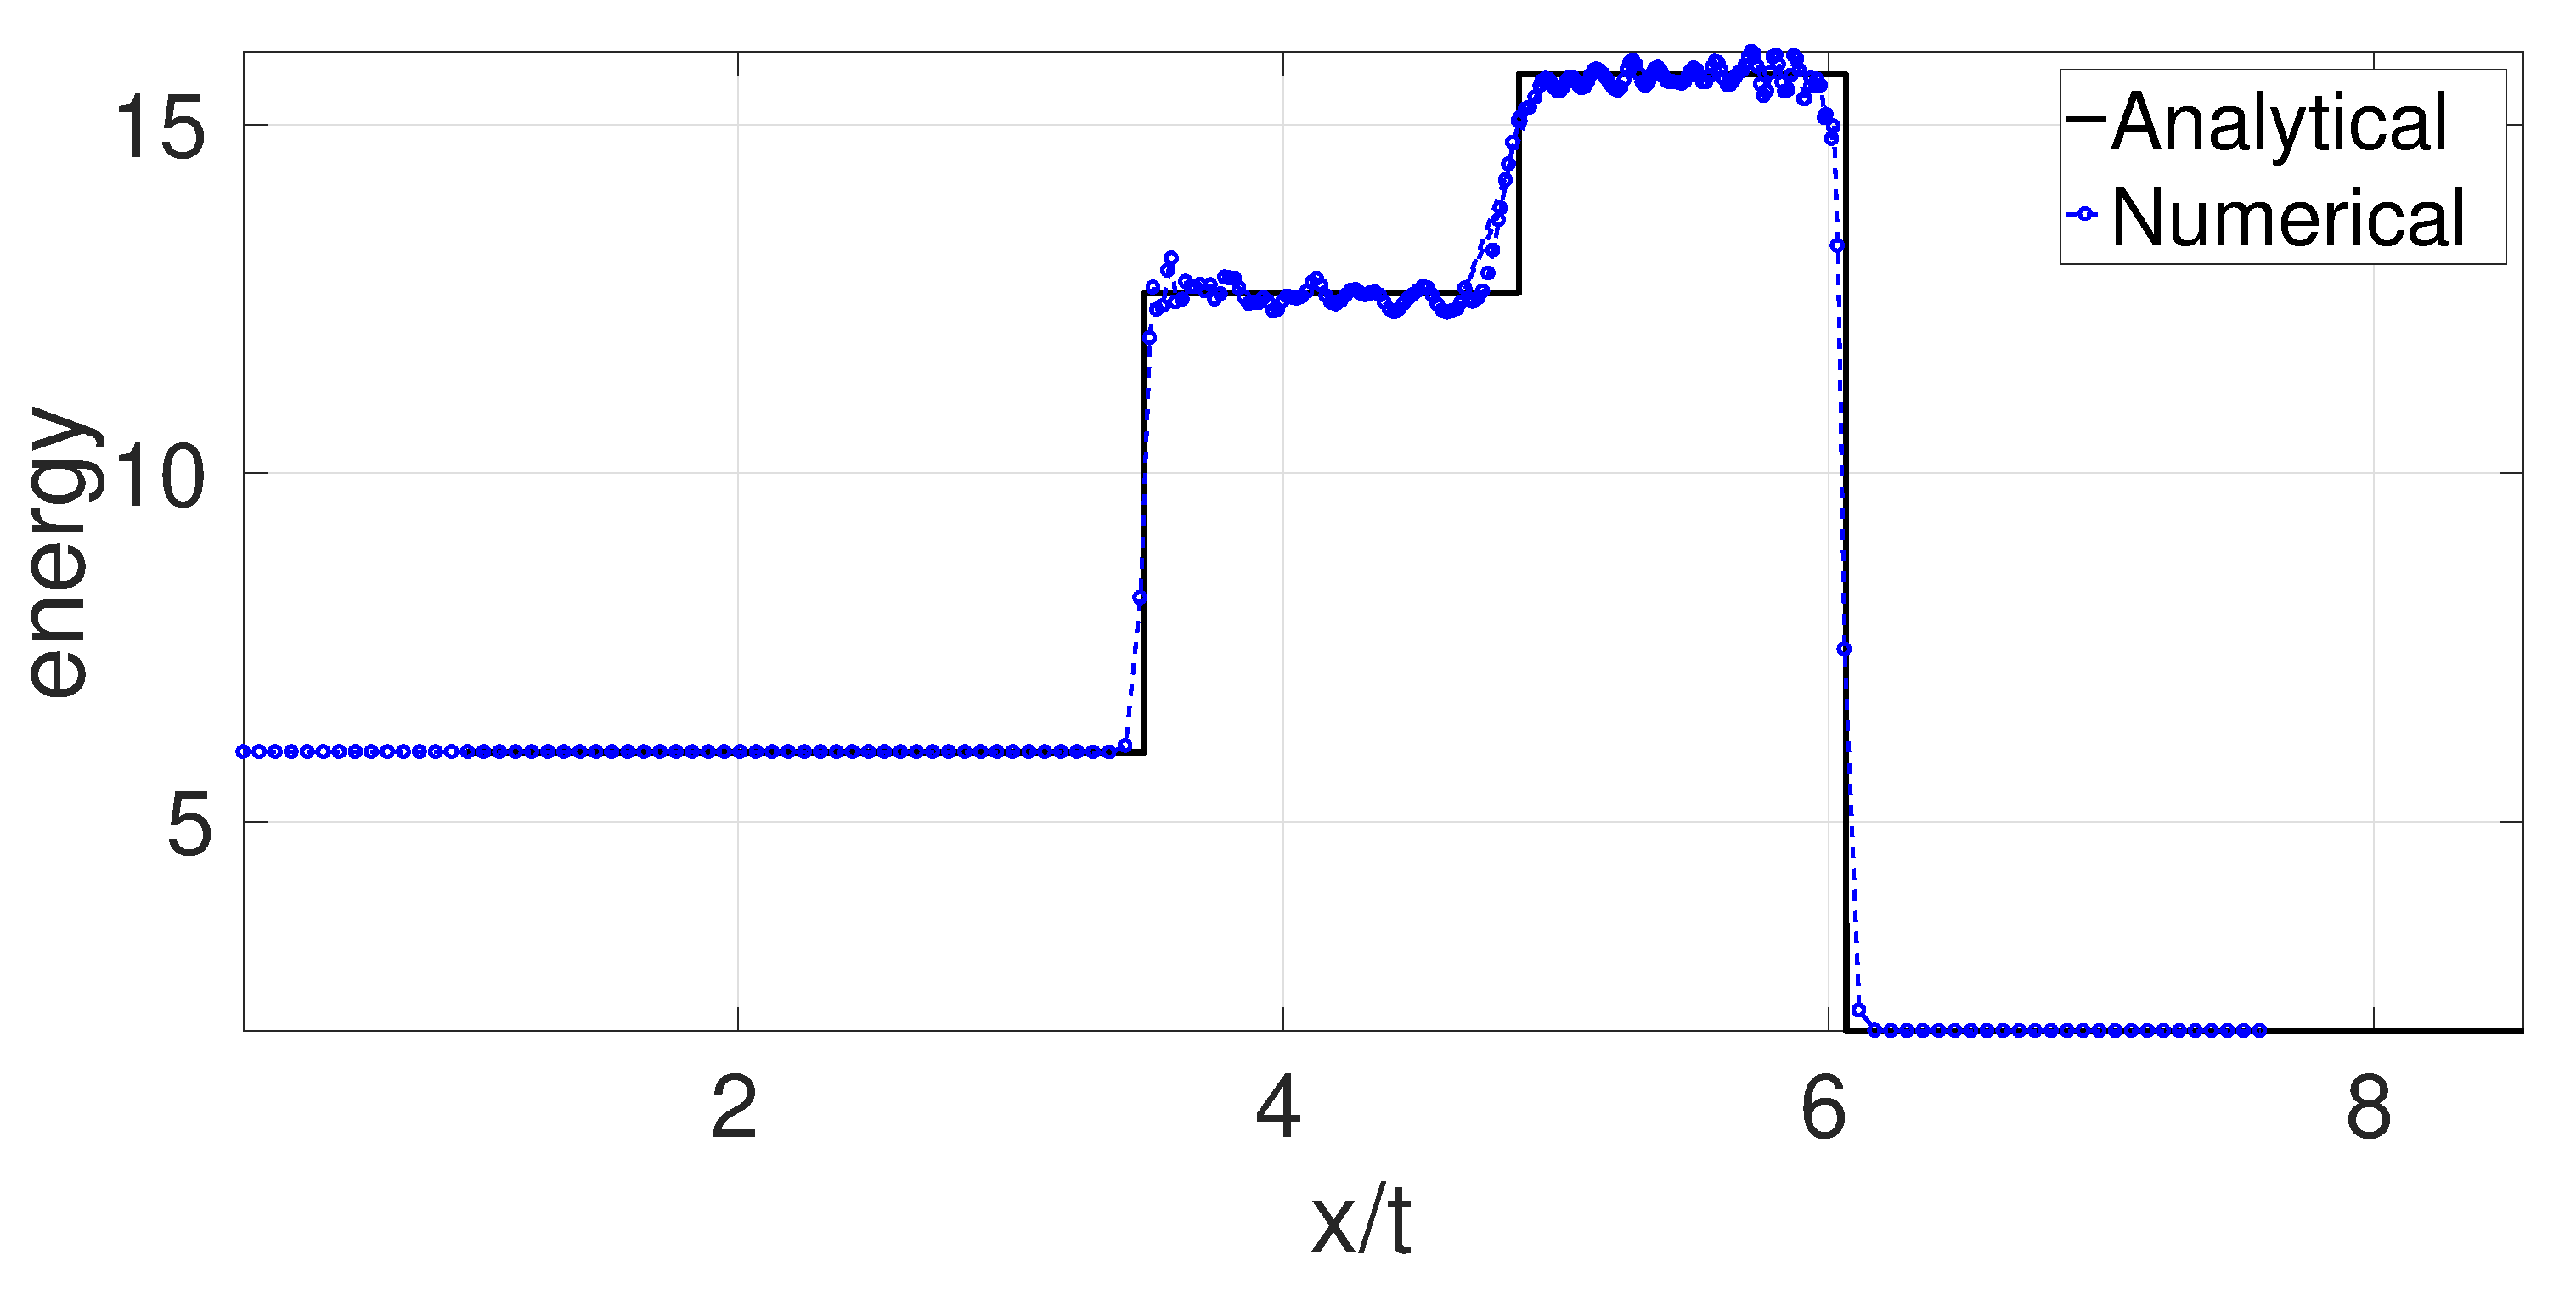
\includegraphics[width=0.99 \textwidth]{./Figures/double_shock/Dshock-RCM-e-Rp6}
    \end{minipage}%
    \begin{minipage}{.495 \textwidth}
        \centering
        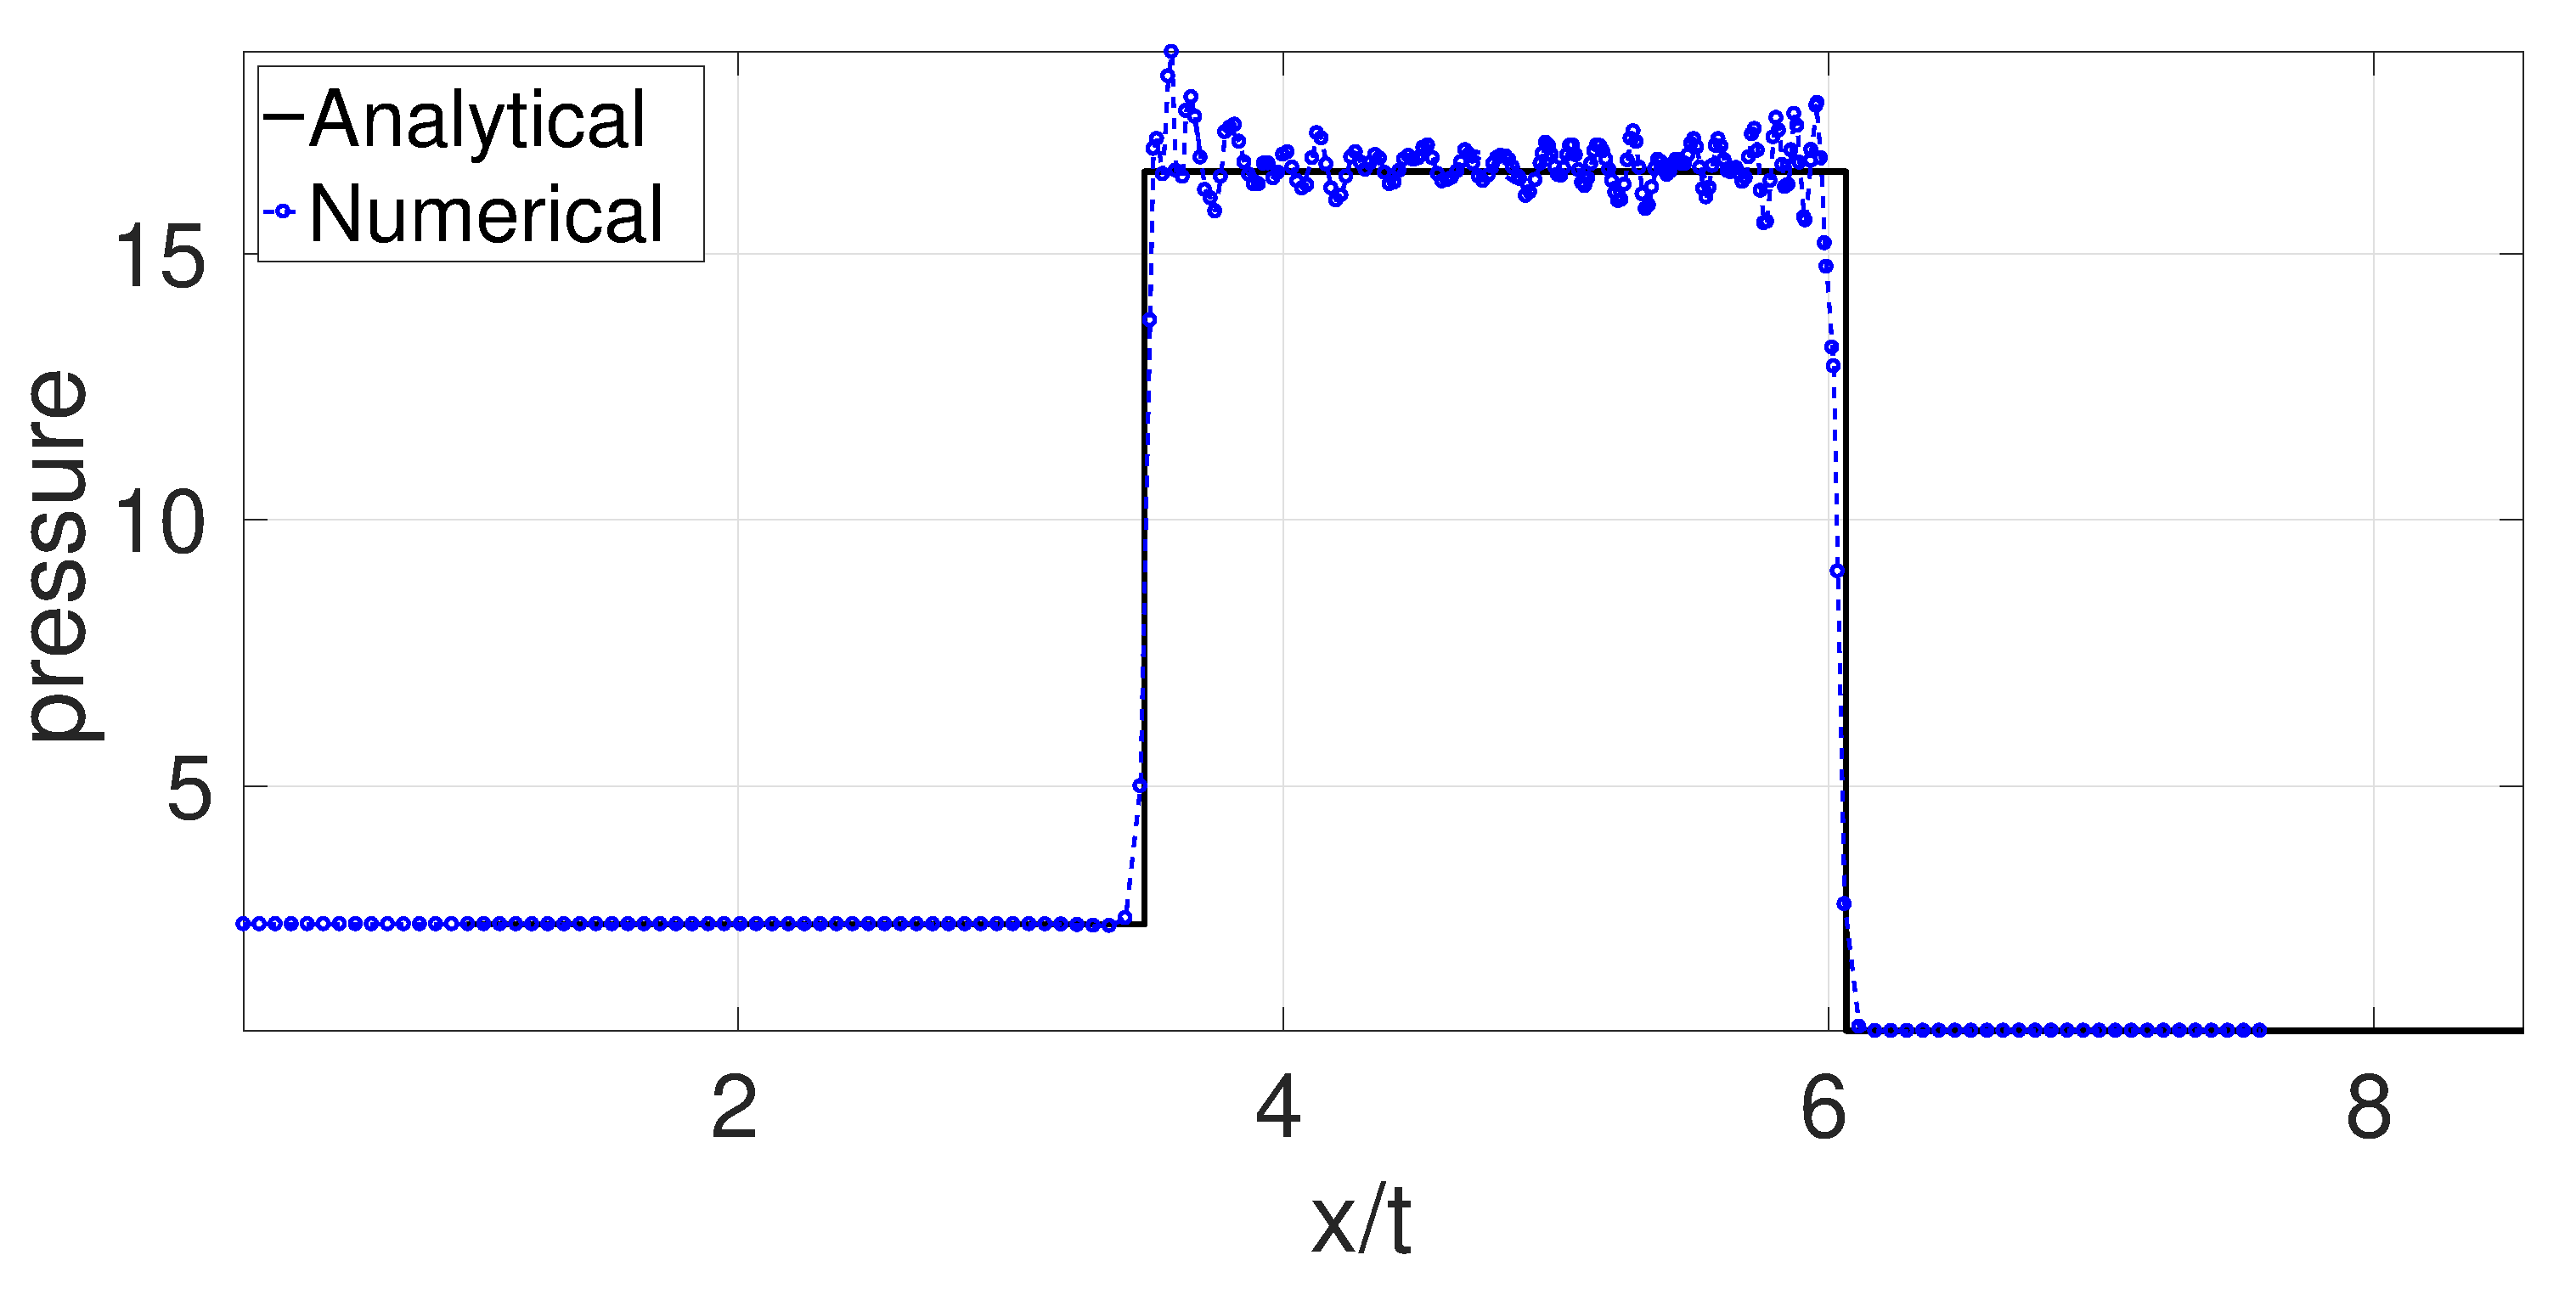
\includegraphics[width=0.99 \textwidth]{./Figures/double_shock/Dshock-RCM-p-Rp6}
    \end{minipage}% 
    \caption{Results for test 4, the double shock case. All physical properties are well re-produced. However, the oscillations are more serious than oscillations in other tests.}
    \label{fig:RCM-double-shock}
\end{figure}

\begin{figure}[H]
    %\centering
    \begin{minipage}{.495\textwidth}
        \centering
        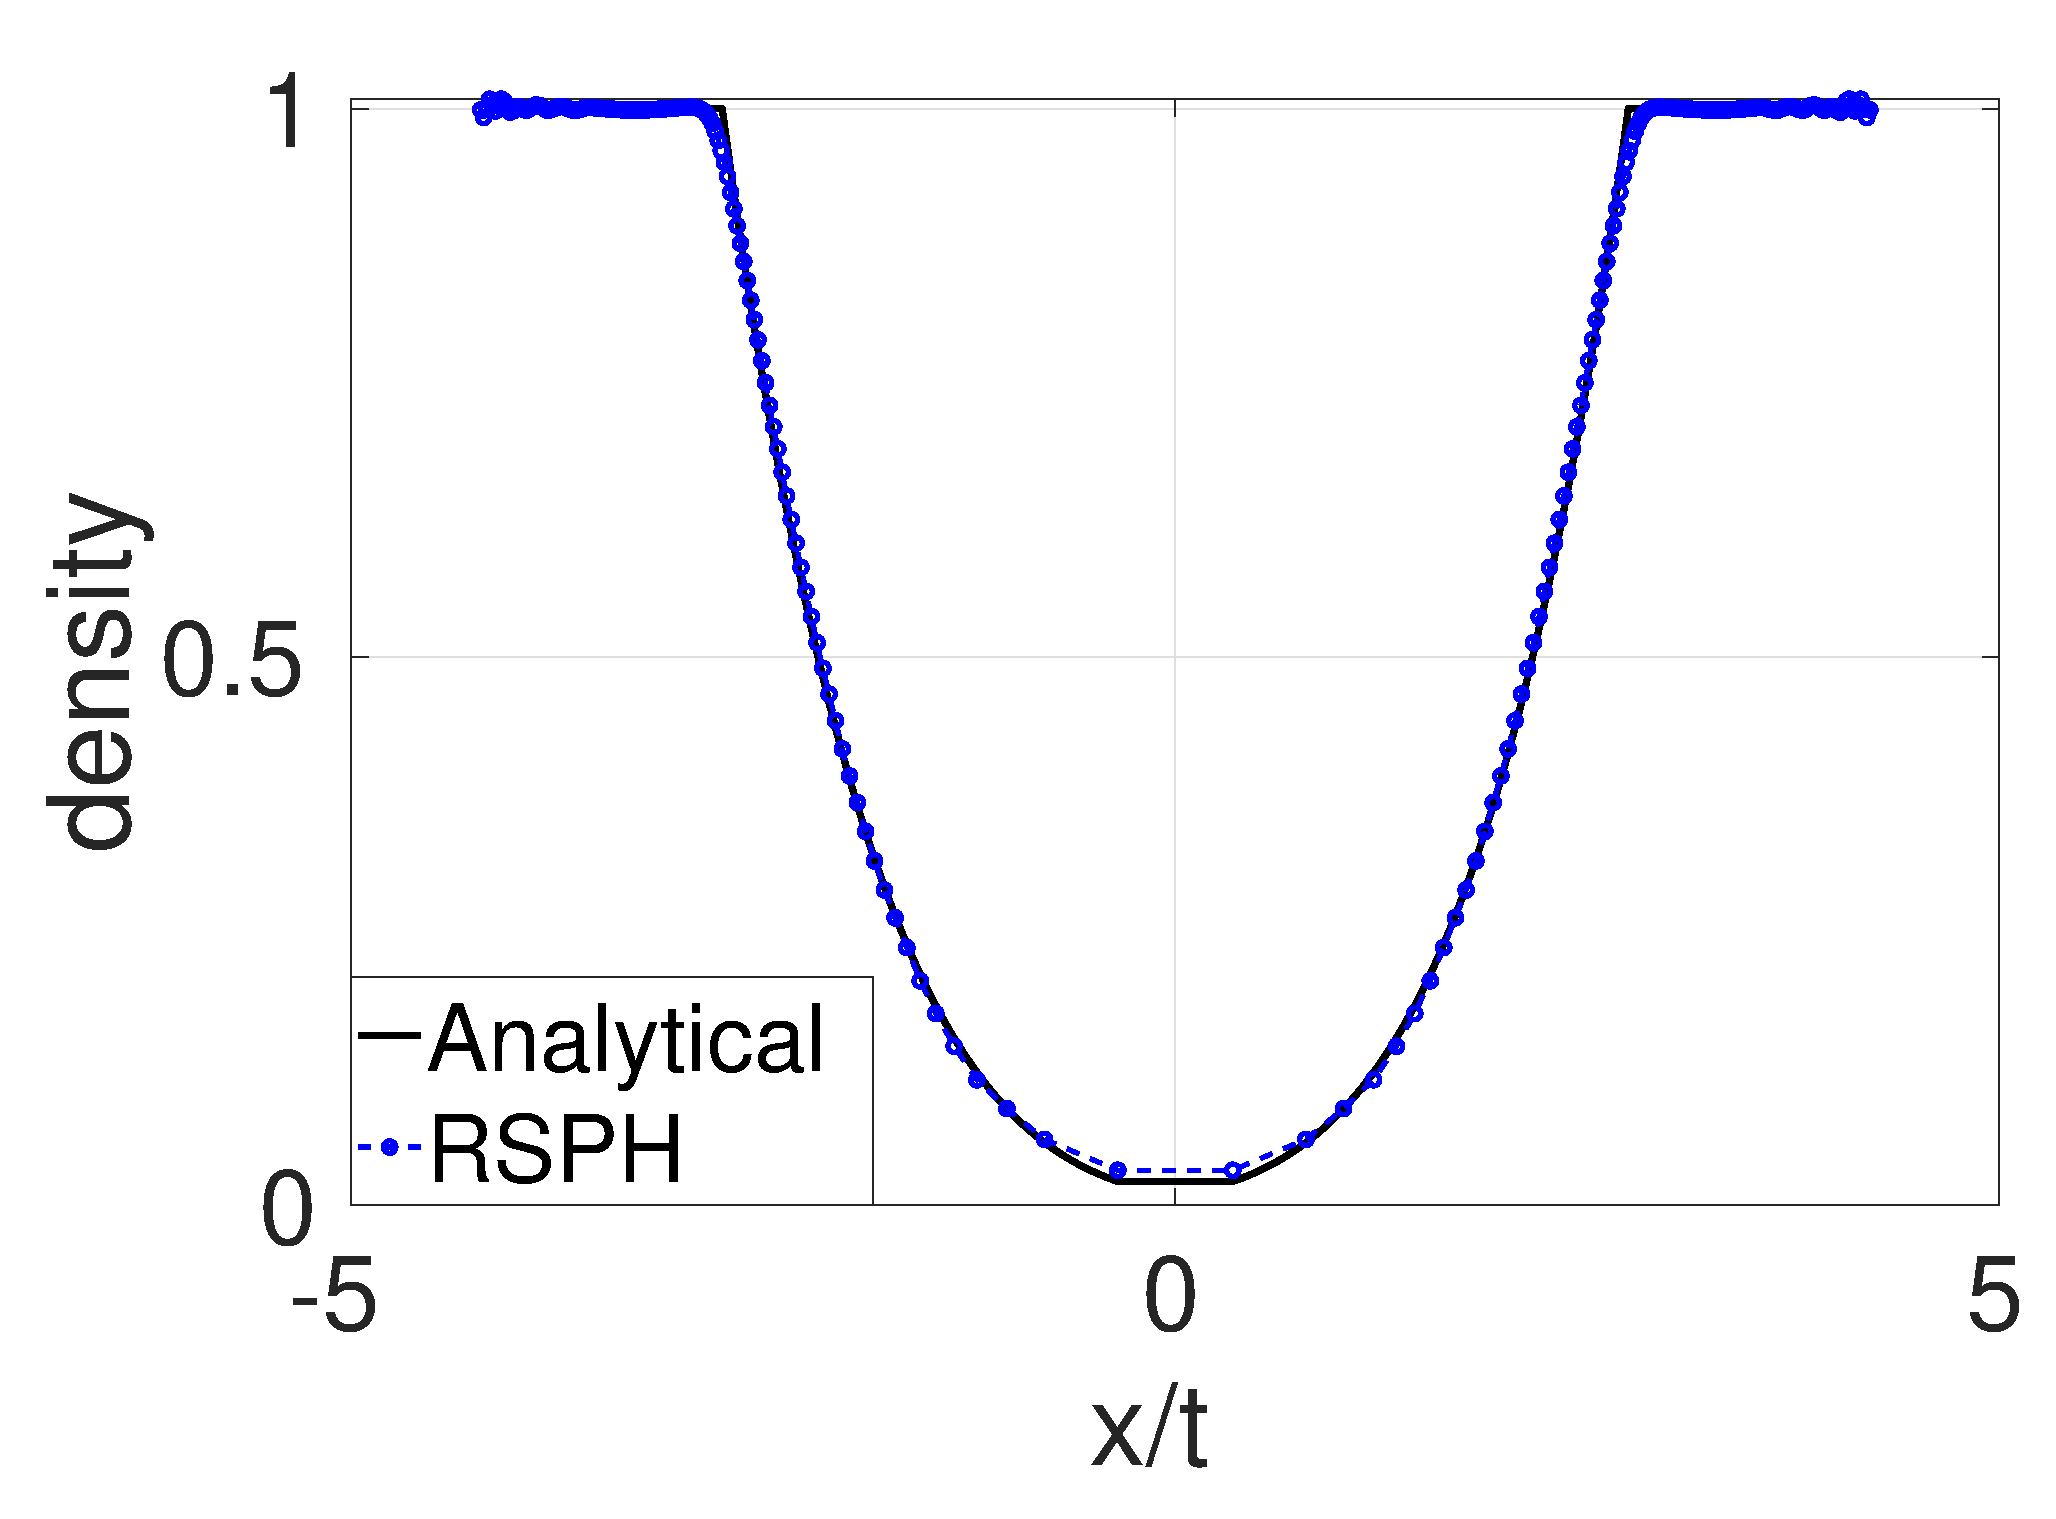
\includegraphics[width=0.99 \textwidth]{./Figures/Sjogreen/Sjogreen-RCM-rho-Adpt1}
    \end{minipage}%
    \begin{minipage}{.495 \textwidth}
        \centering
        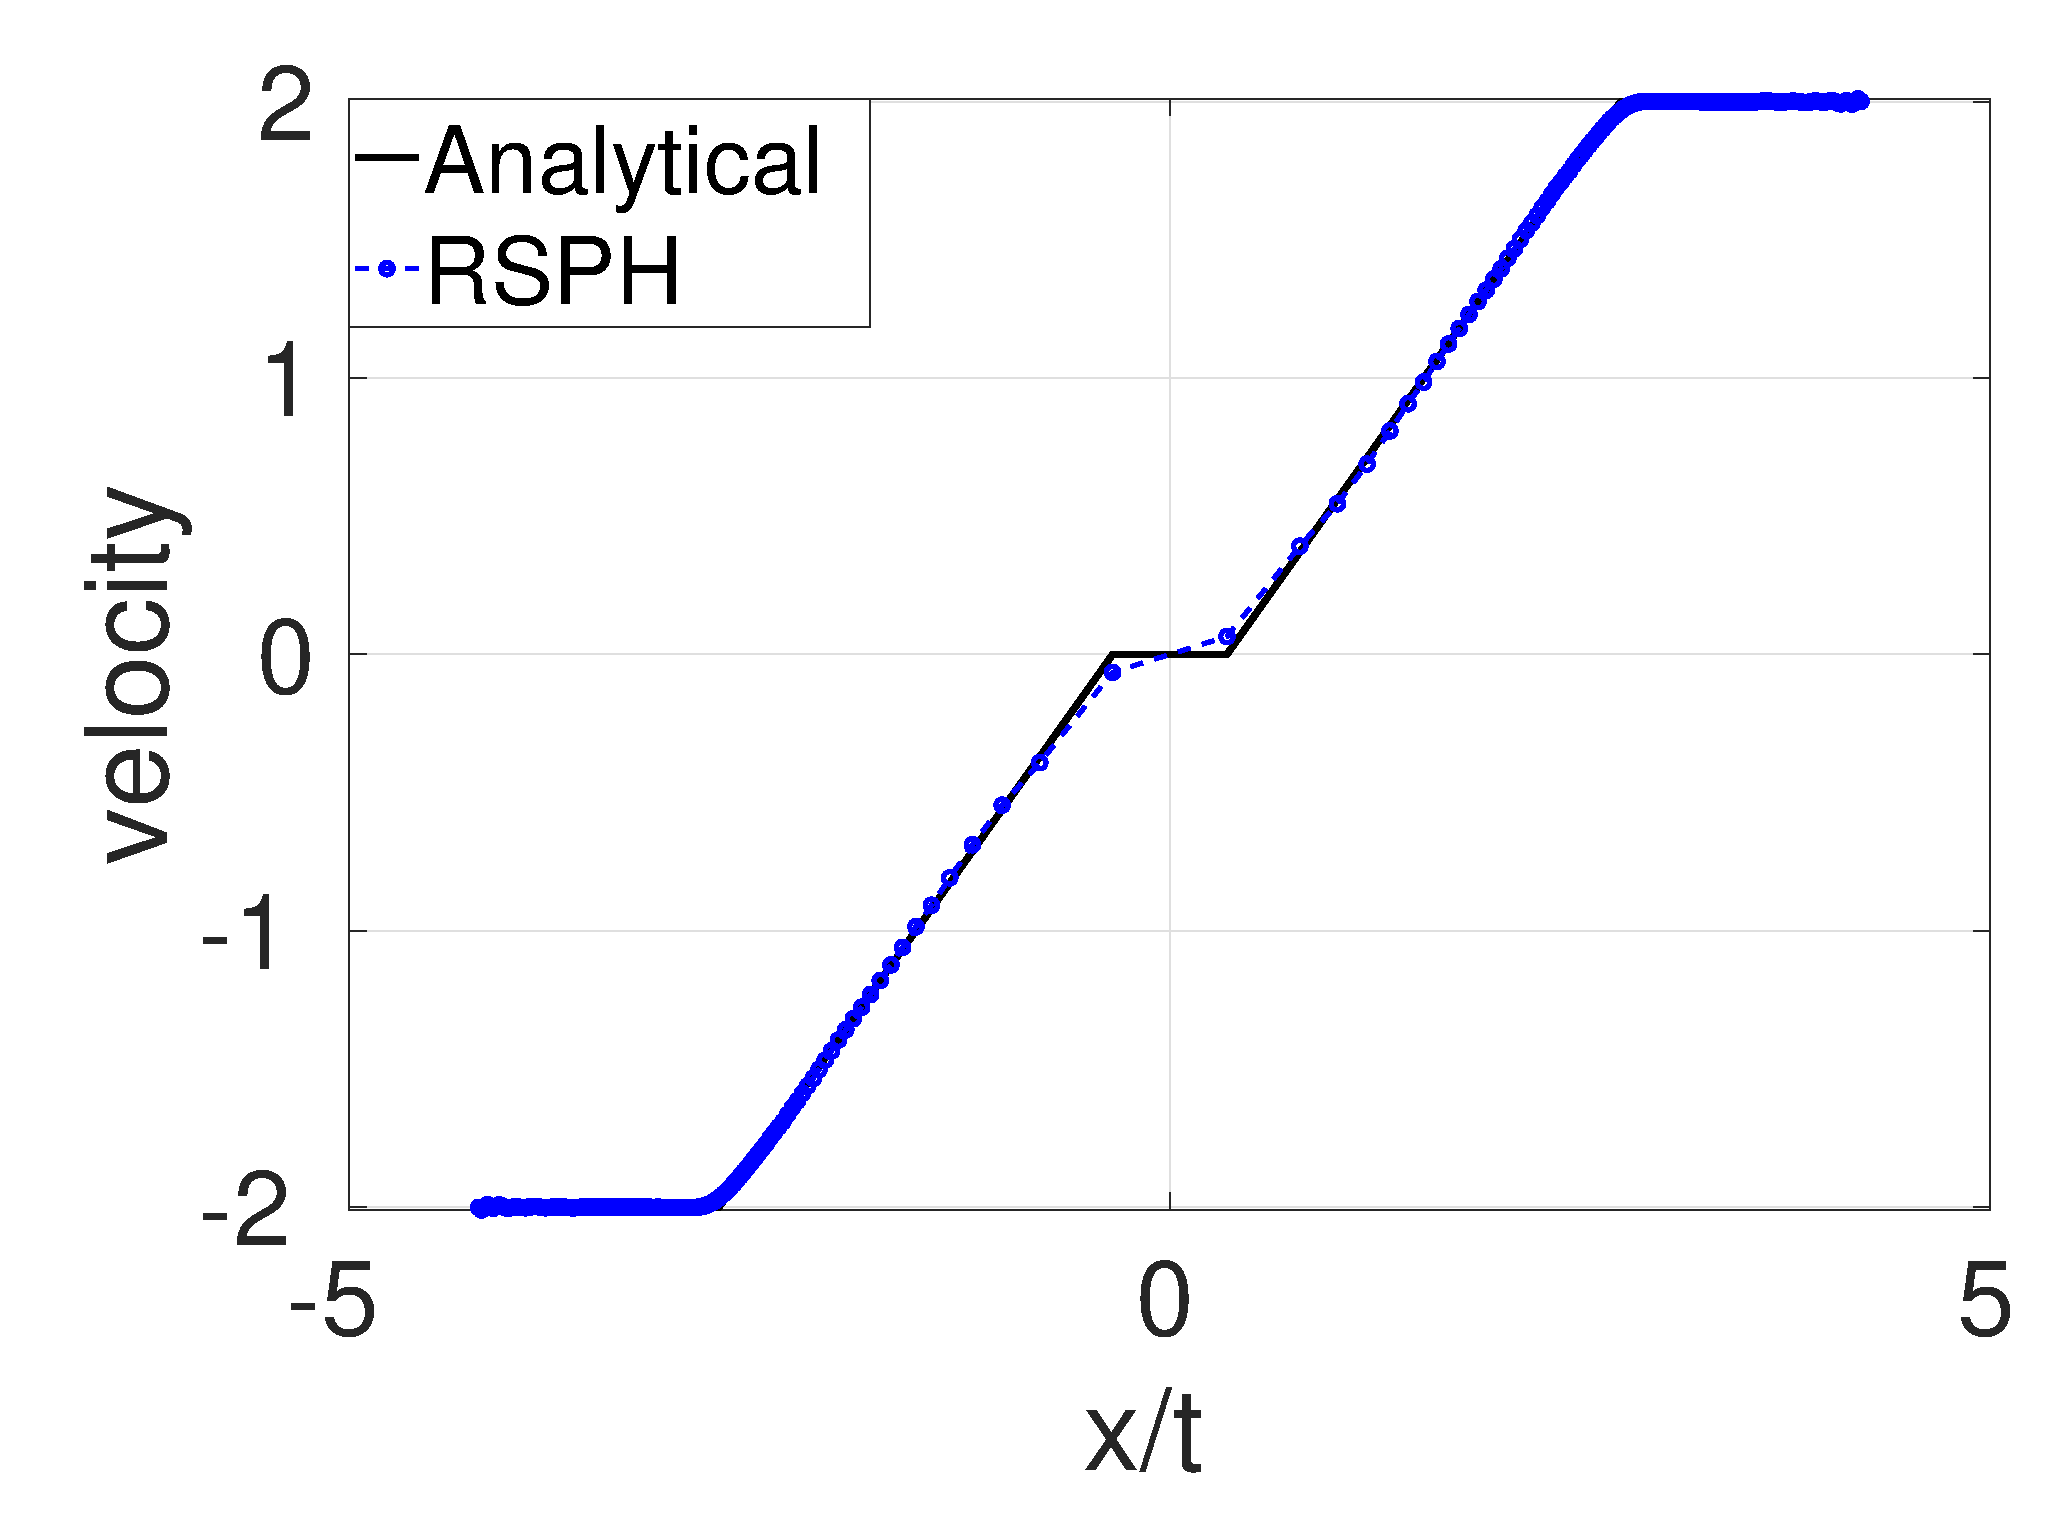
\includegraphics[width=0.99 \textwidth]{./Figures/Sjogreen/Sjogreen-RCM-v-Adpt1}
    \end{minipage}%
    \\
    \begin{minipage}{.495\textwidth}
        \centering
        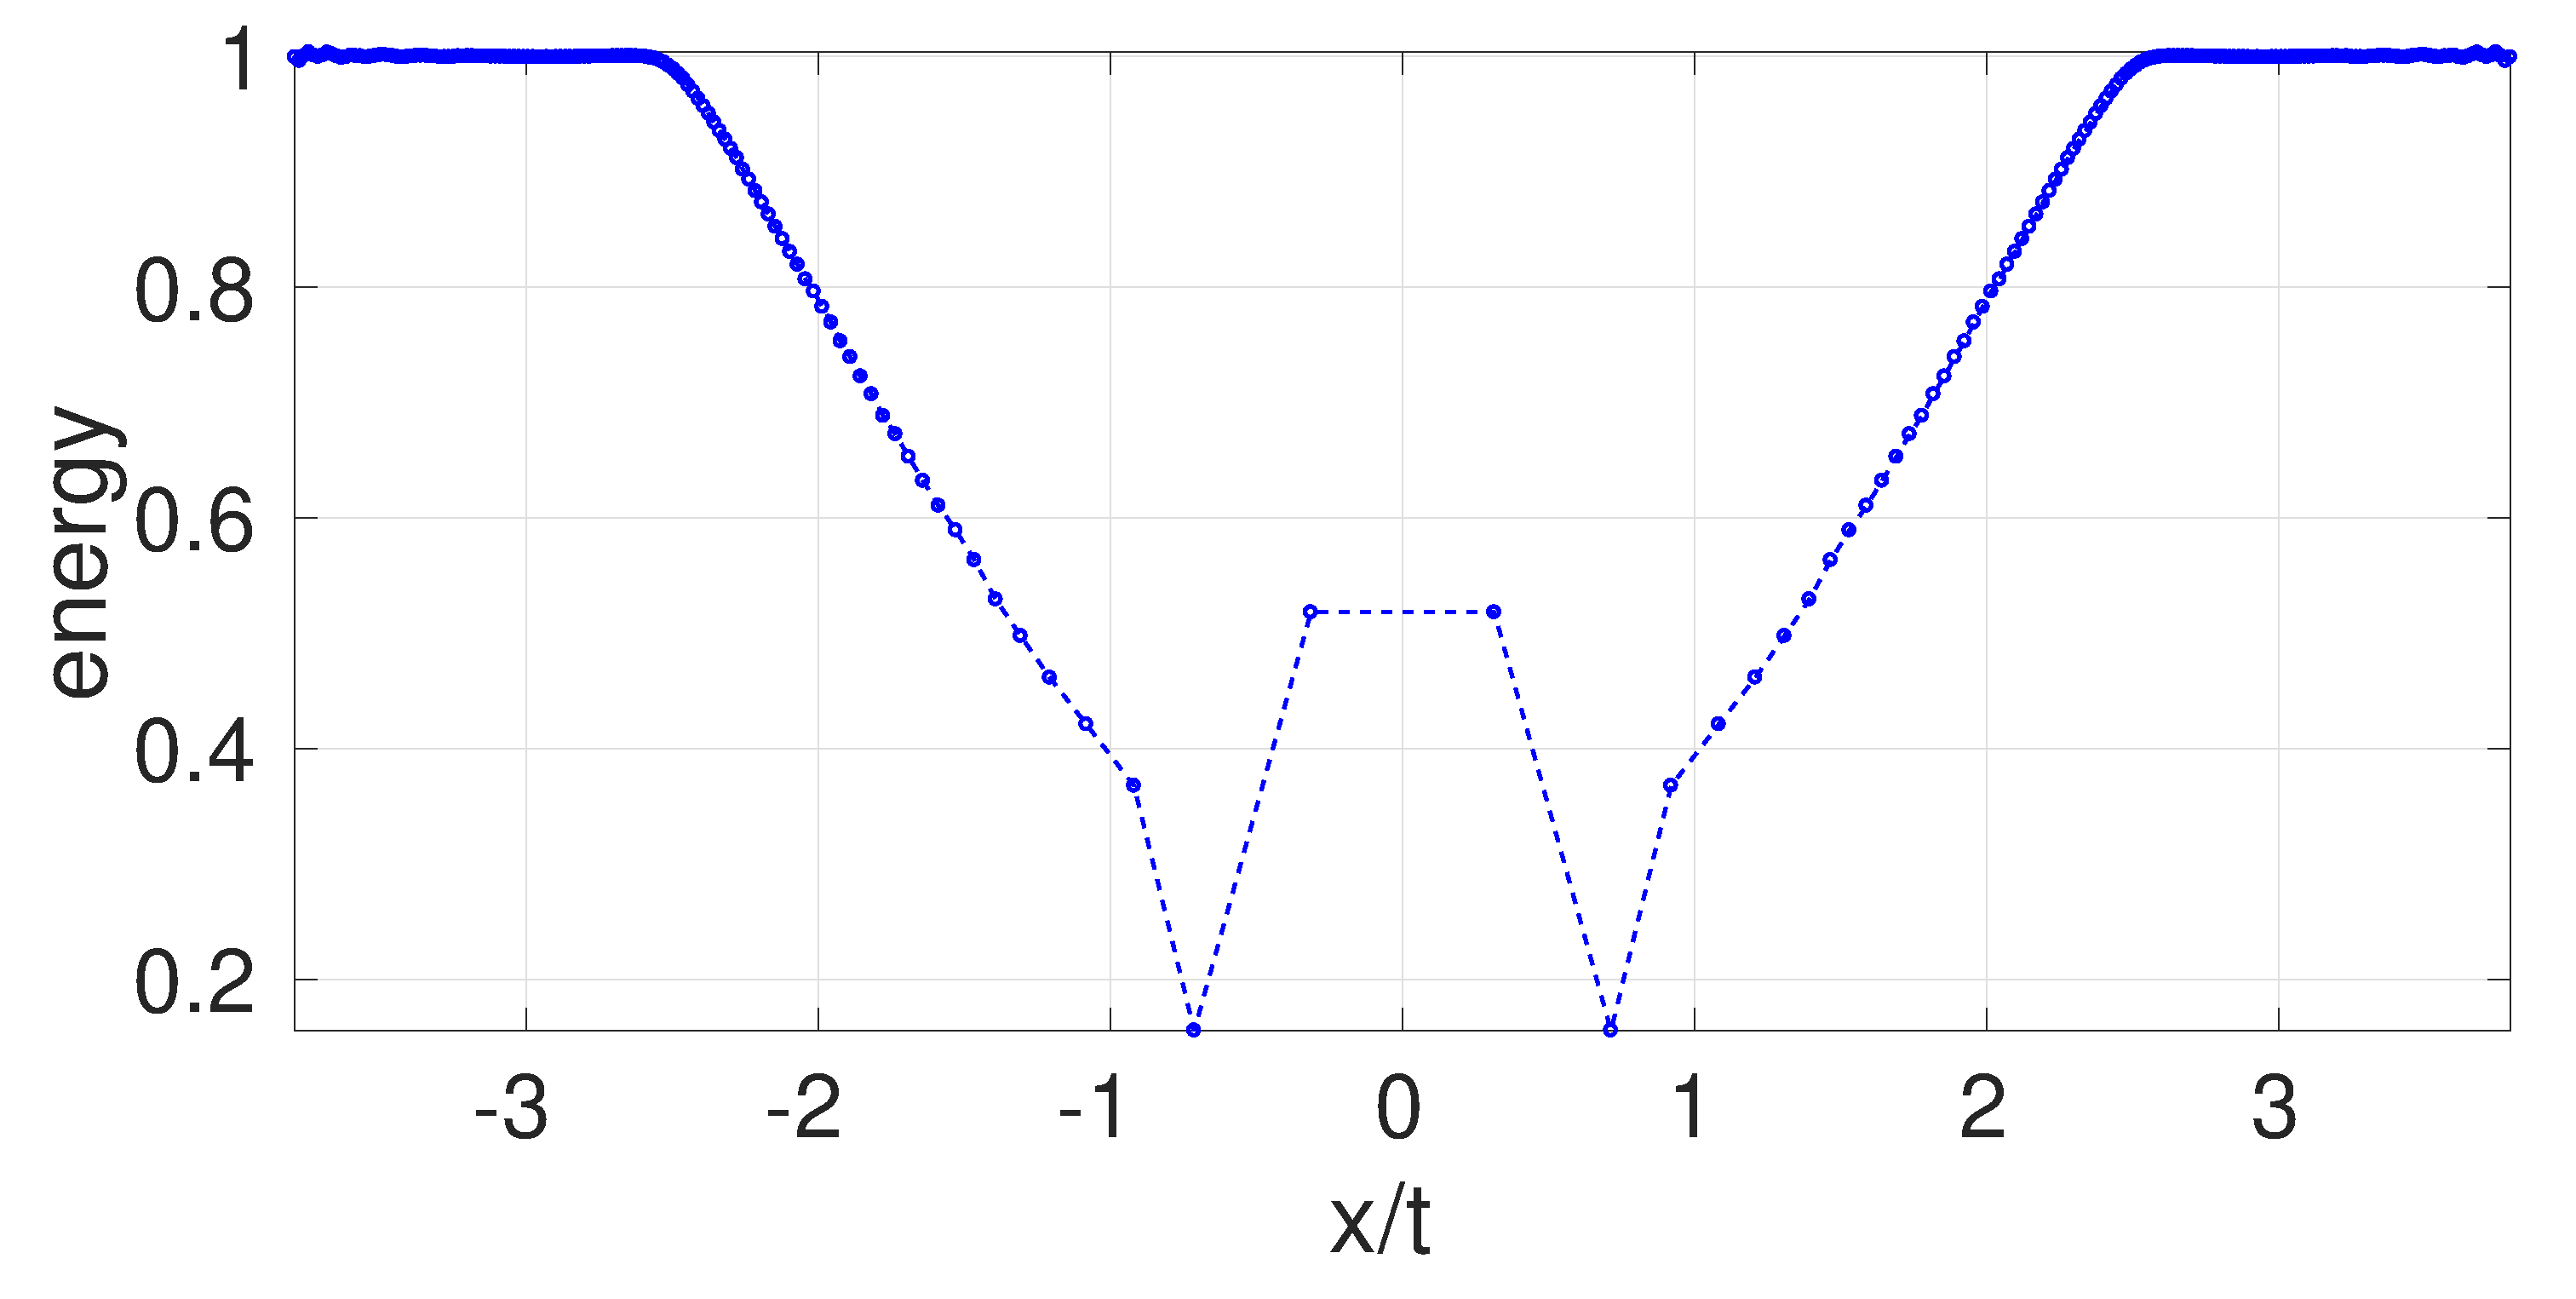
\includegraphics[width=0.99 \textwidth]{./Figures/Sjogreen/Sjogreen-RCM-e-Adpt1}
    \end{minipage}%
    \begin{minipage}{.495 \textwidth}
        \centering
        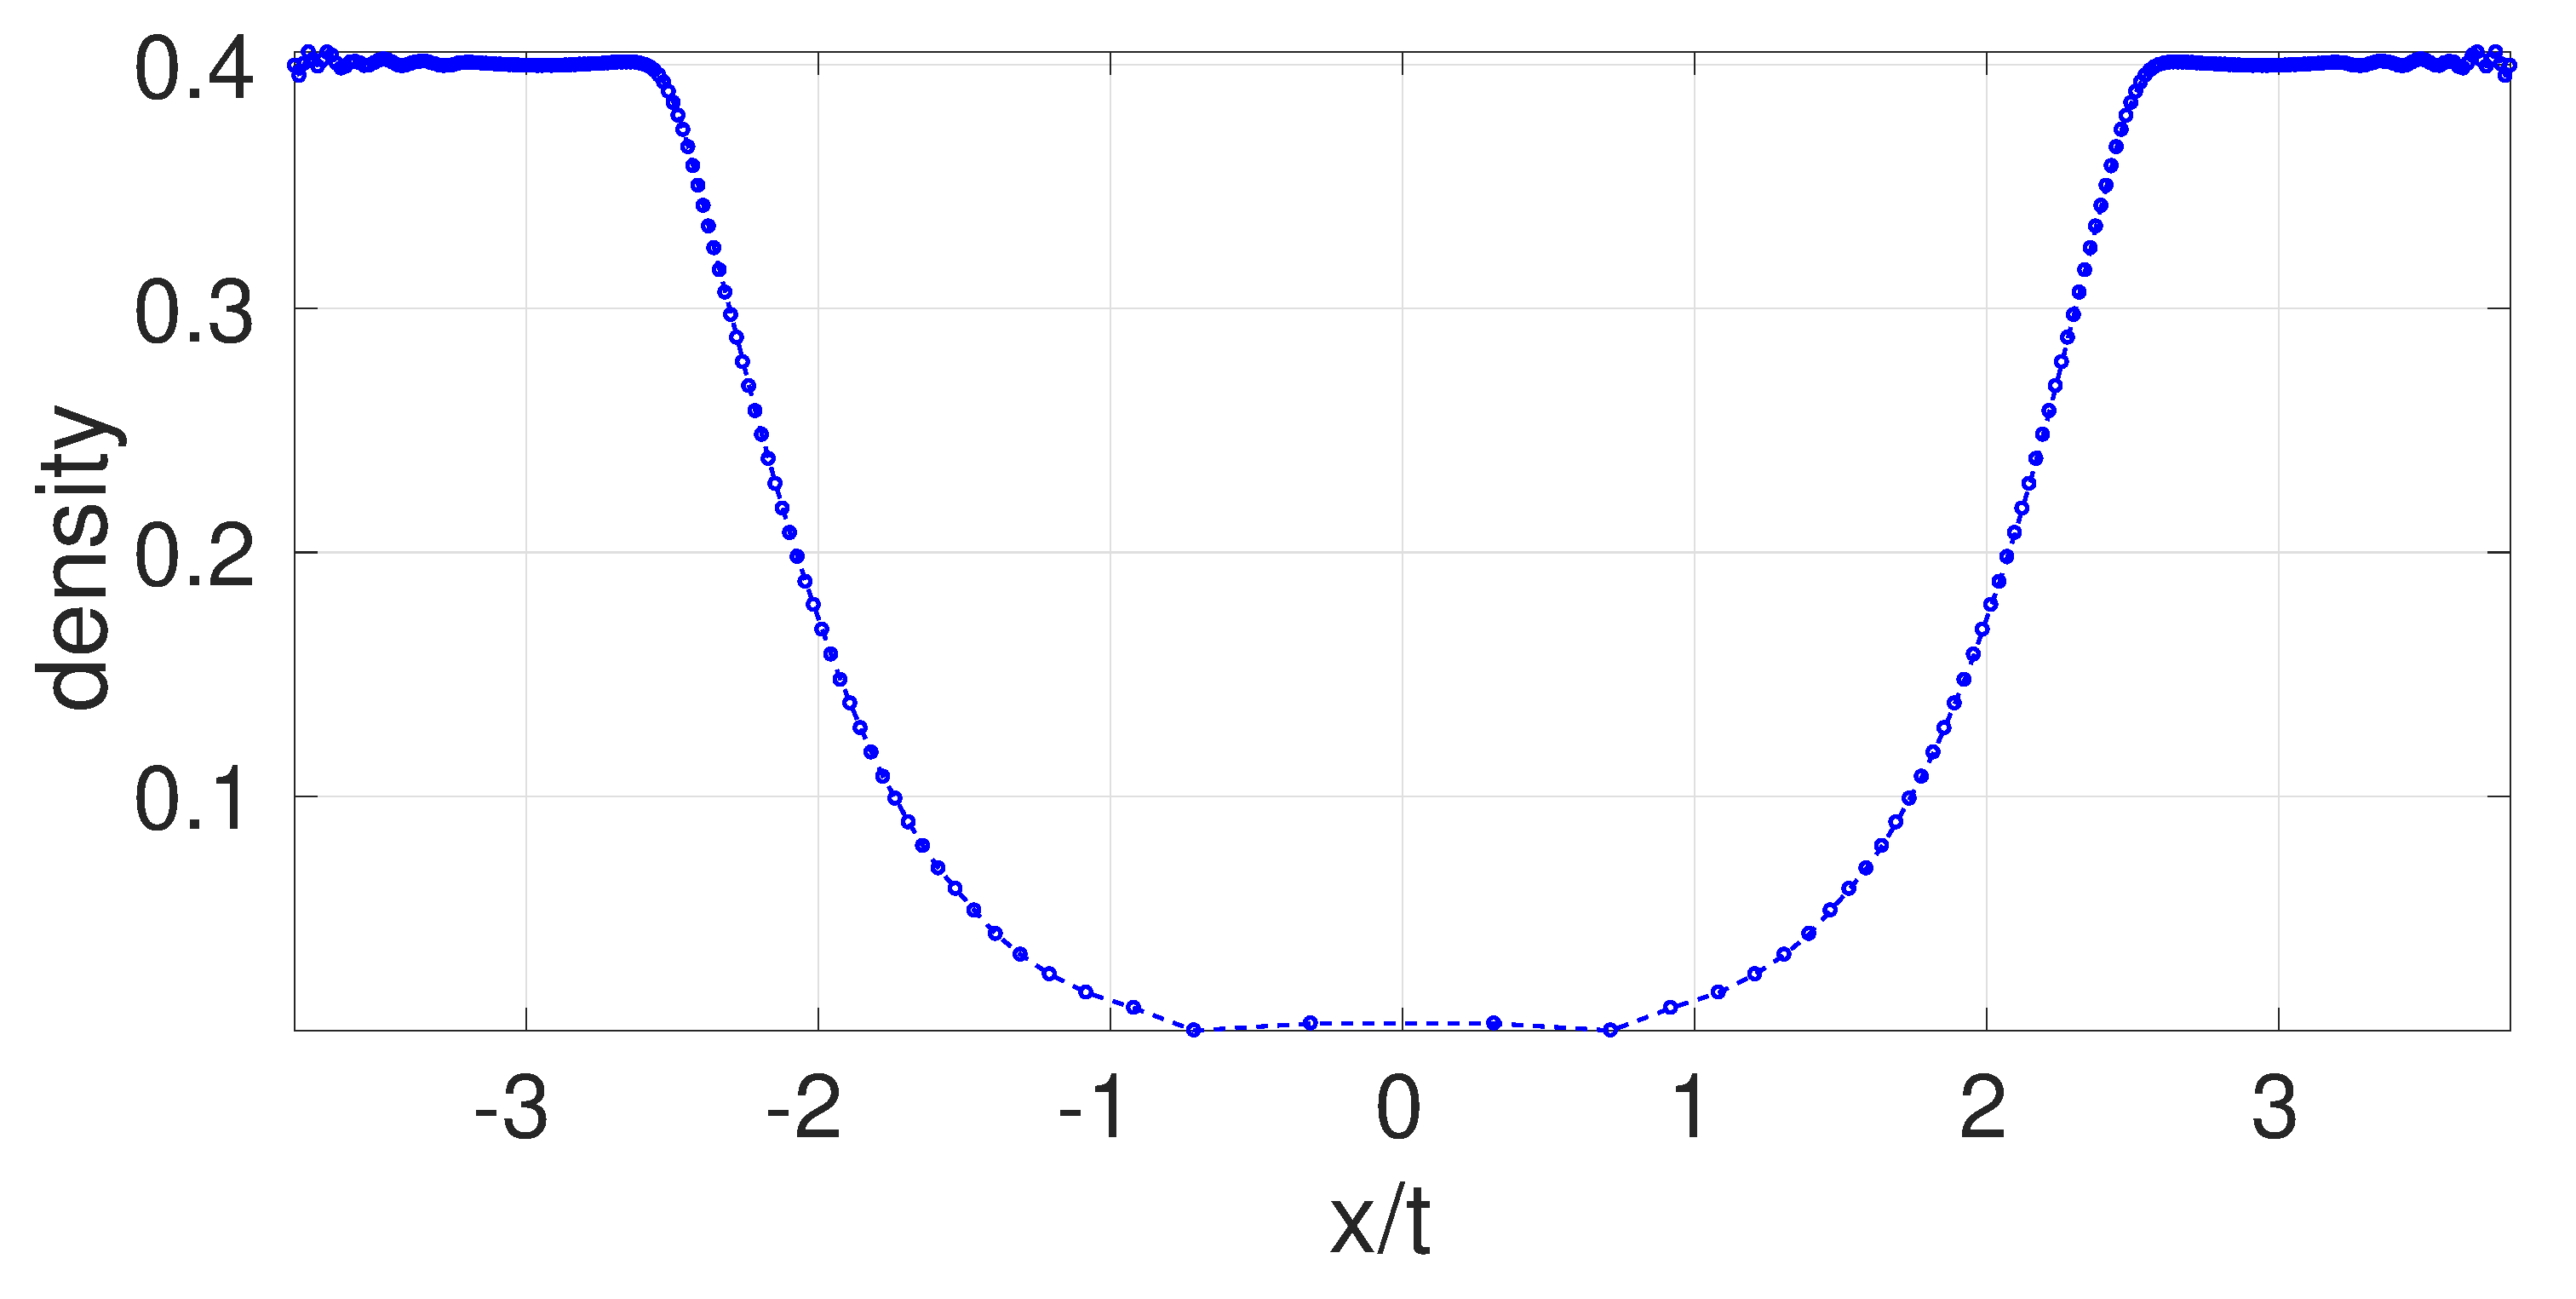
\includegraphics[width=0.99 \textwidth]{./Figures/Sjogreen/Sjogreen-RCM-p-Adpt1}
    \end{minipage}% 
    \caption{Results for test 5, a variation of the Sjogreen test. The density, velocity and pressure are well re-produced while the thermal energy at the origin is poorly predict. A jump of internal energy at the origin is a common issue in many SPH schemes (see, for example, \citep{monaghan1997sph,cha2003implementations,puri2014approximate})}
    \label{fig:RCM-Sjogreen}
\end{figure}

\begin{figure}[H]
    \centering
    \begin{minipage}{.495\textwidth}
        \centering
        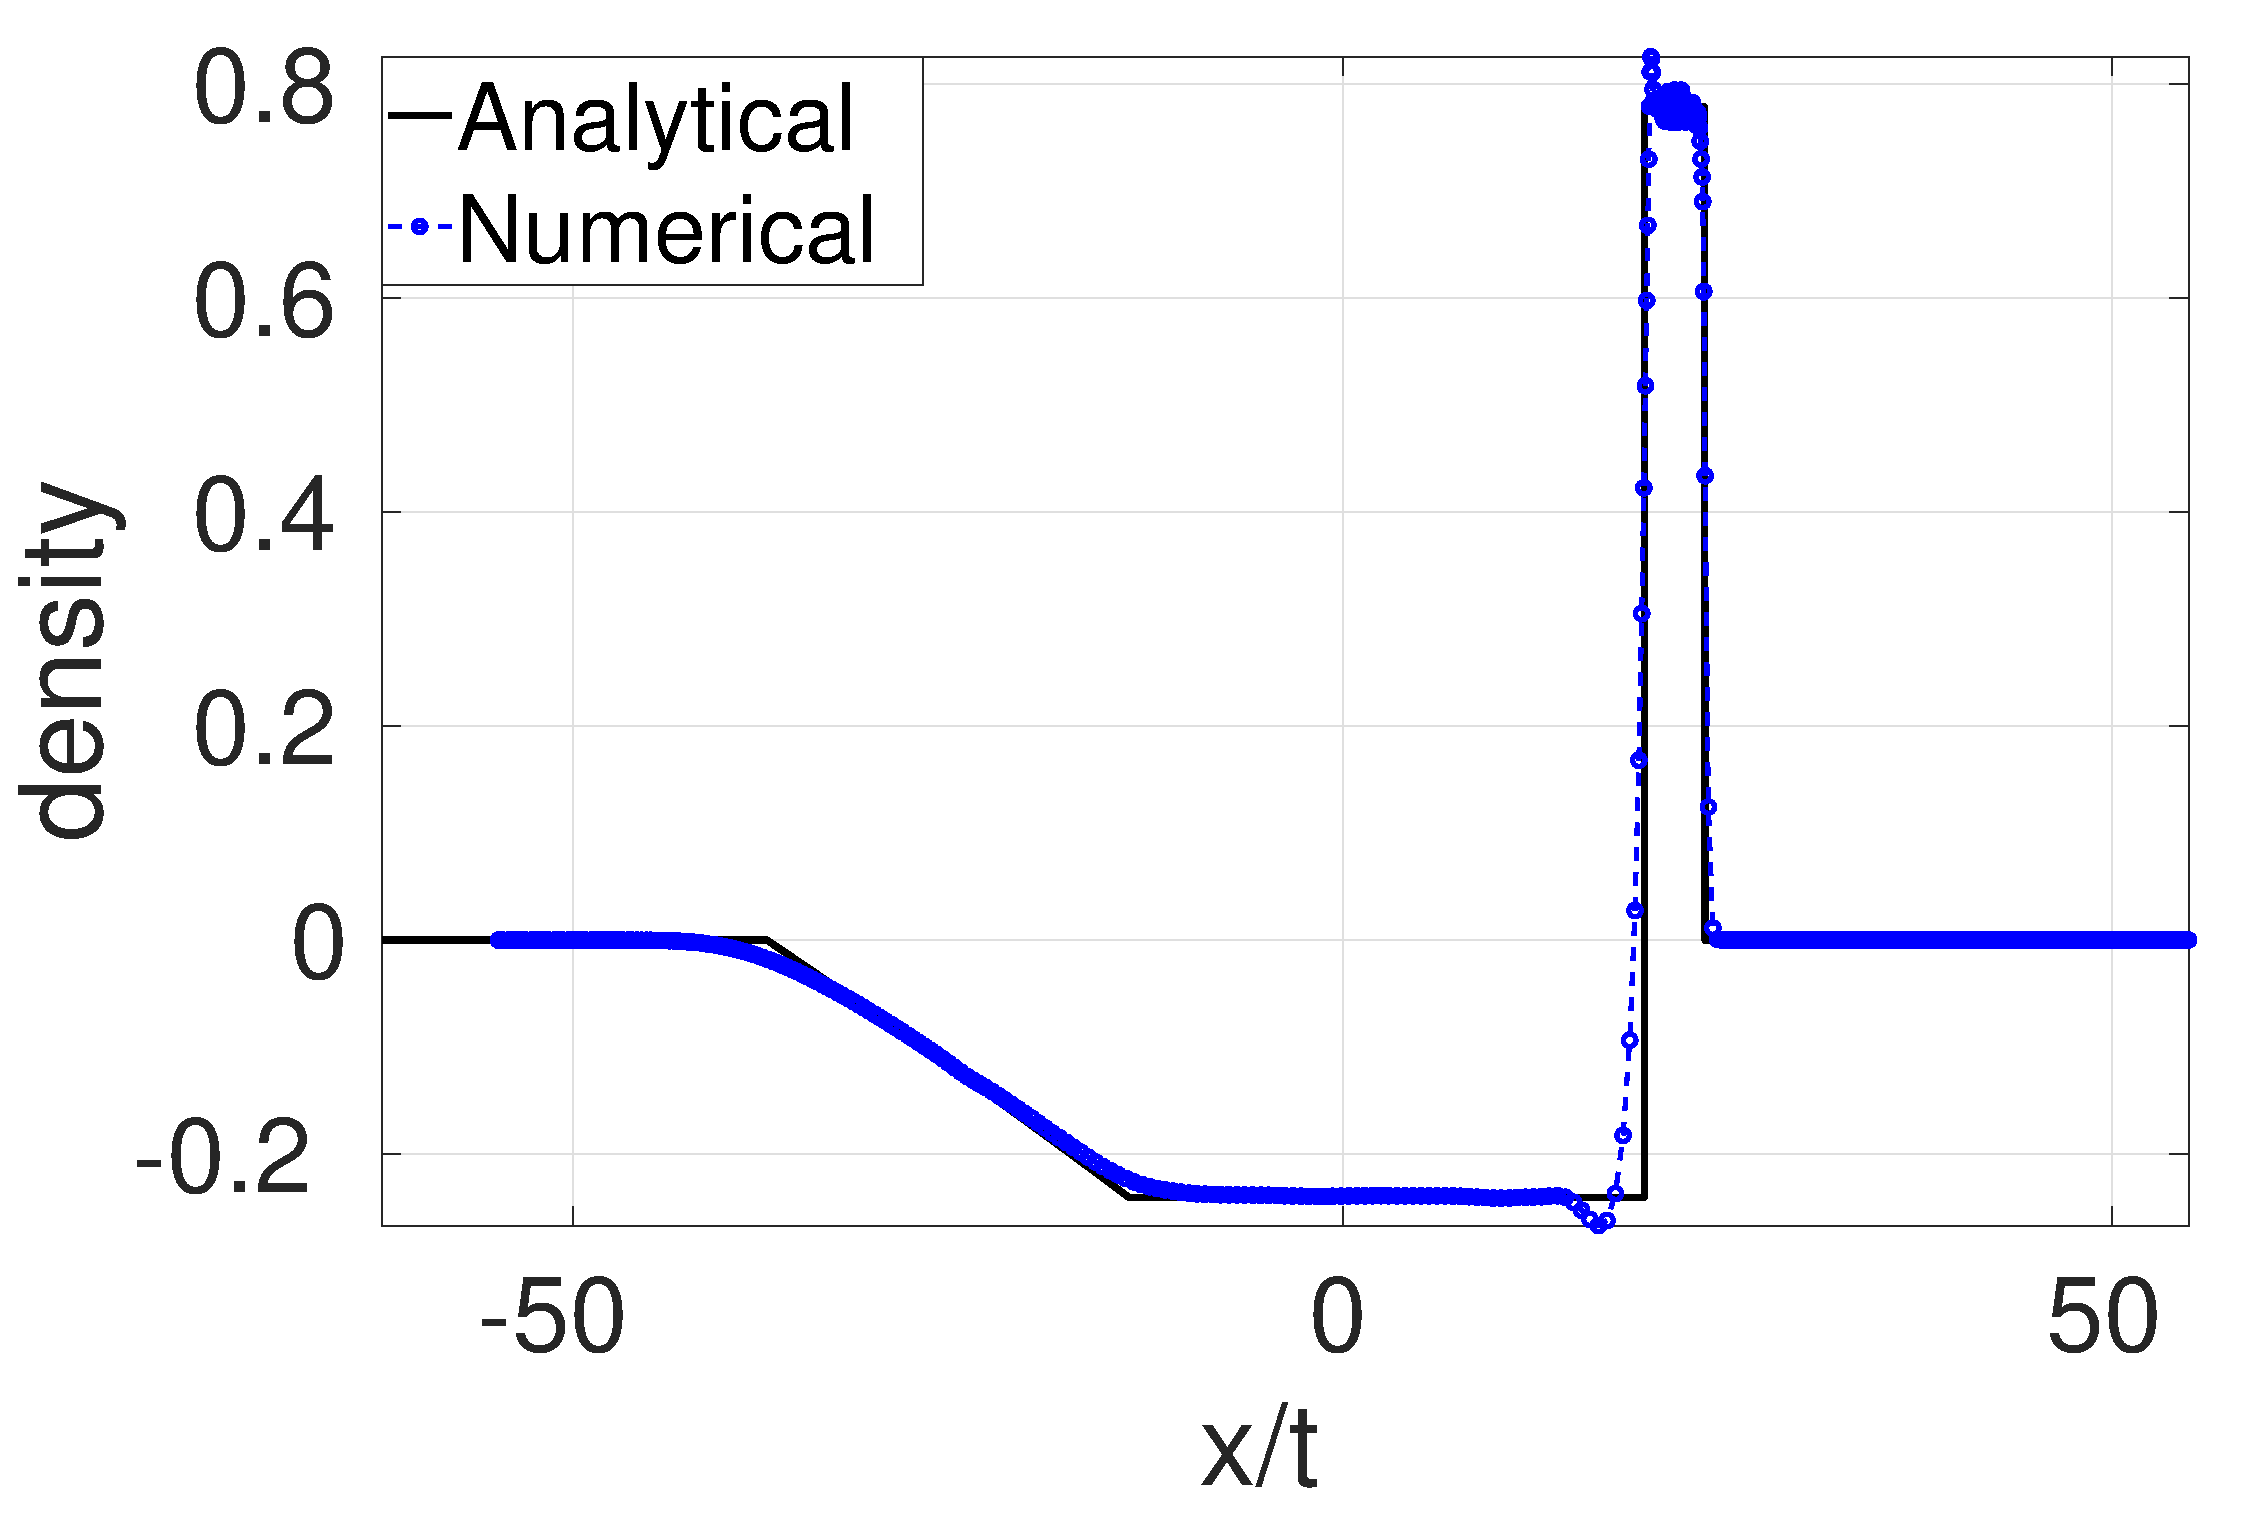
\includegraphics[width=0.99 \textwidth]{./Figures/strong-blast/StrBlst-RCM-rho-Rp3}
    \end{minipage}%
    \begin{minipage}{.495 \textwidth}
        \centering
        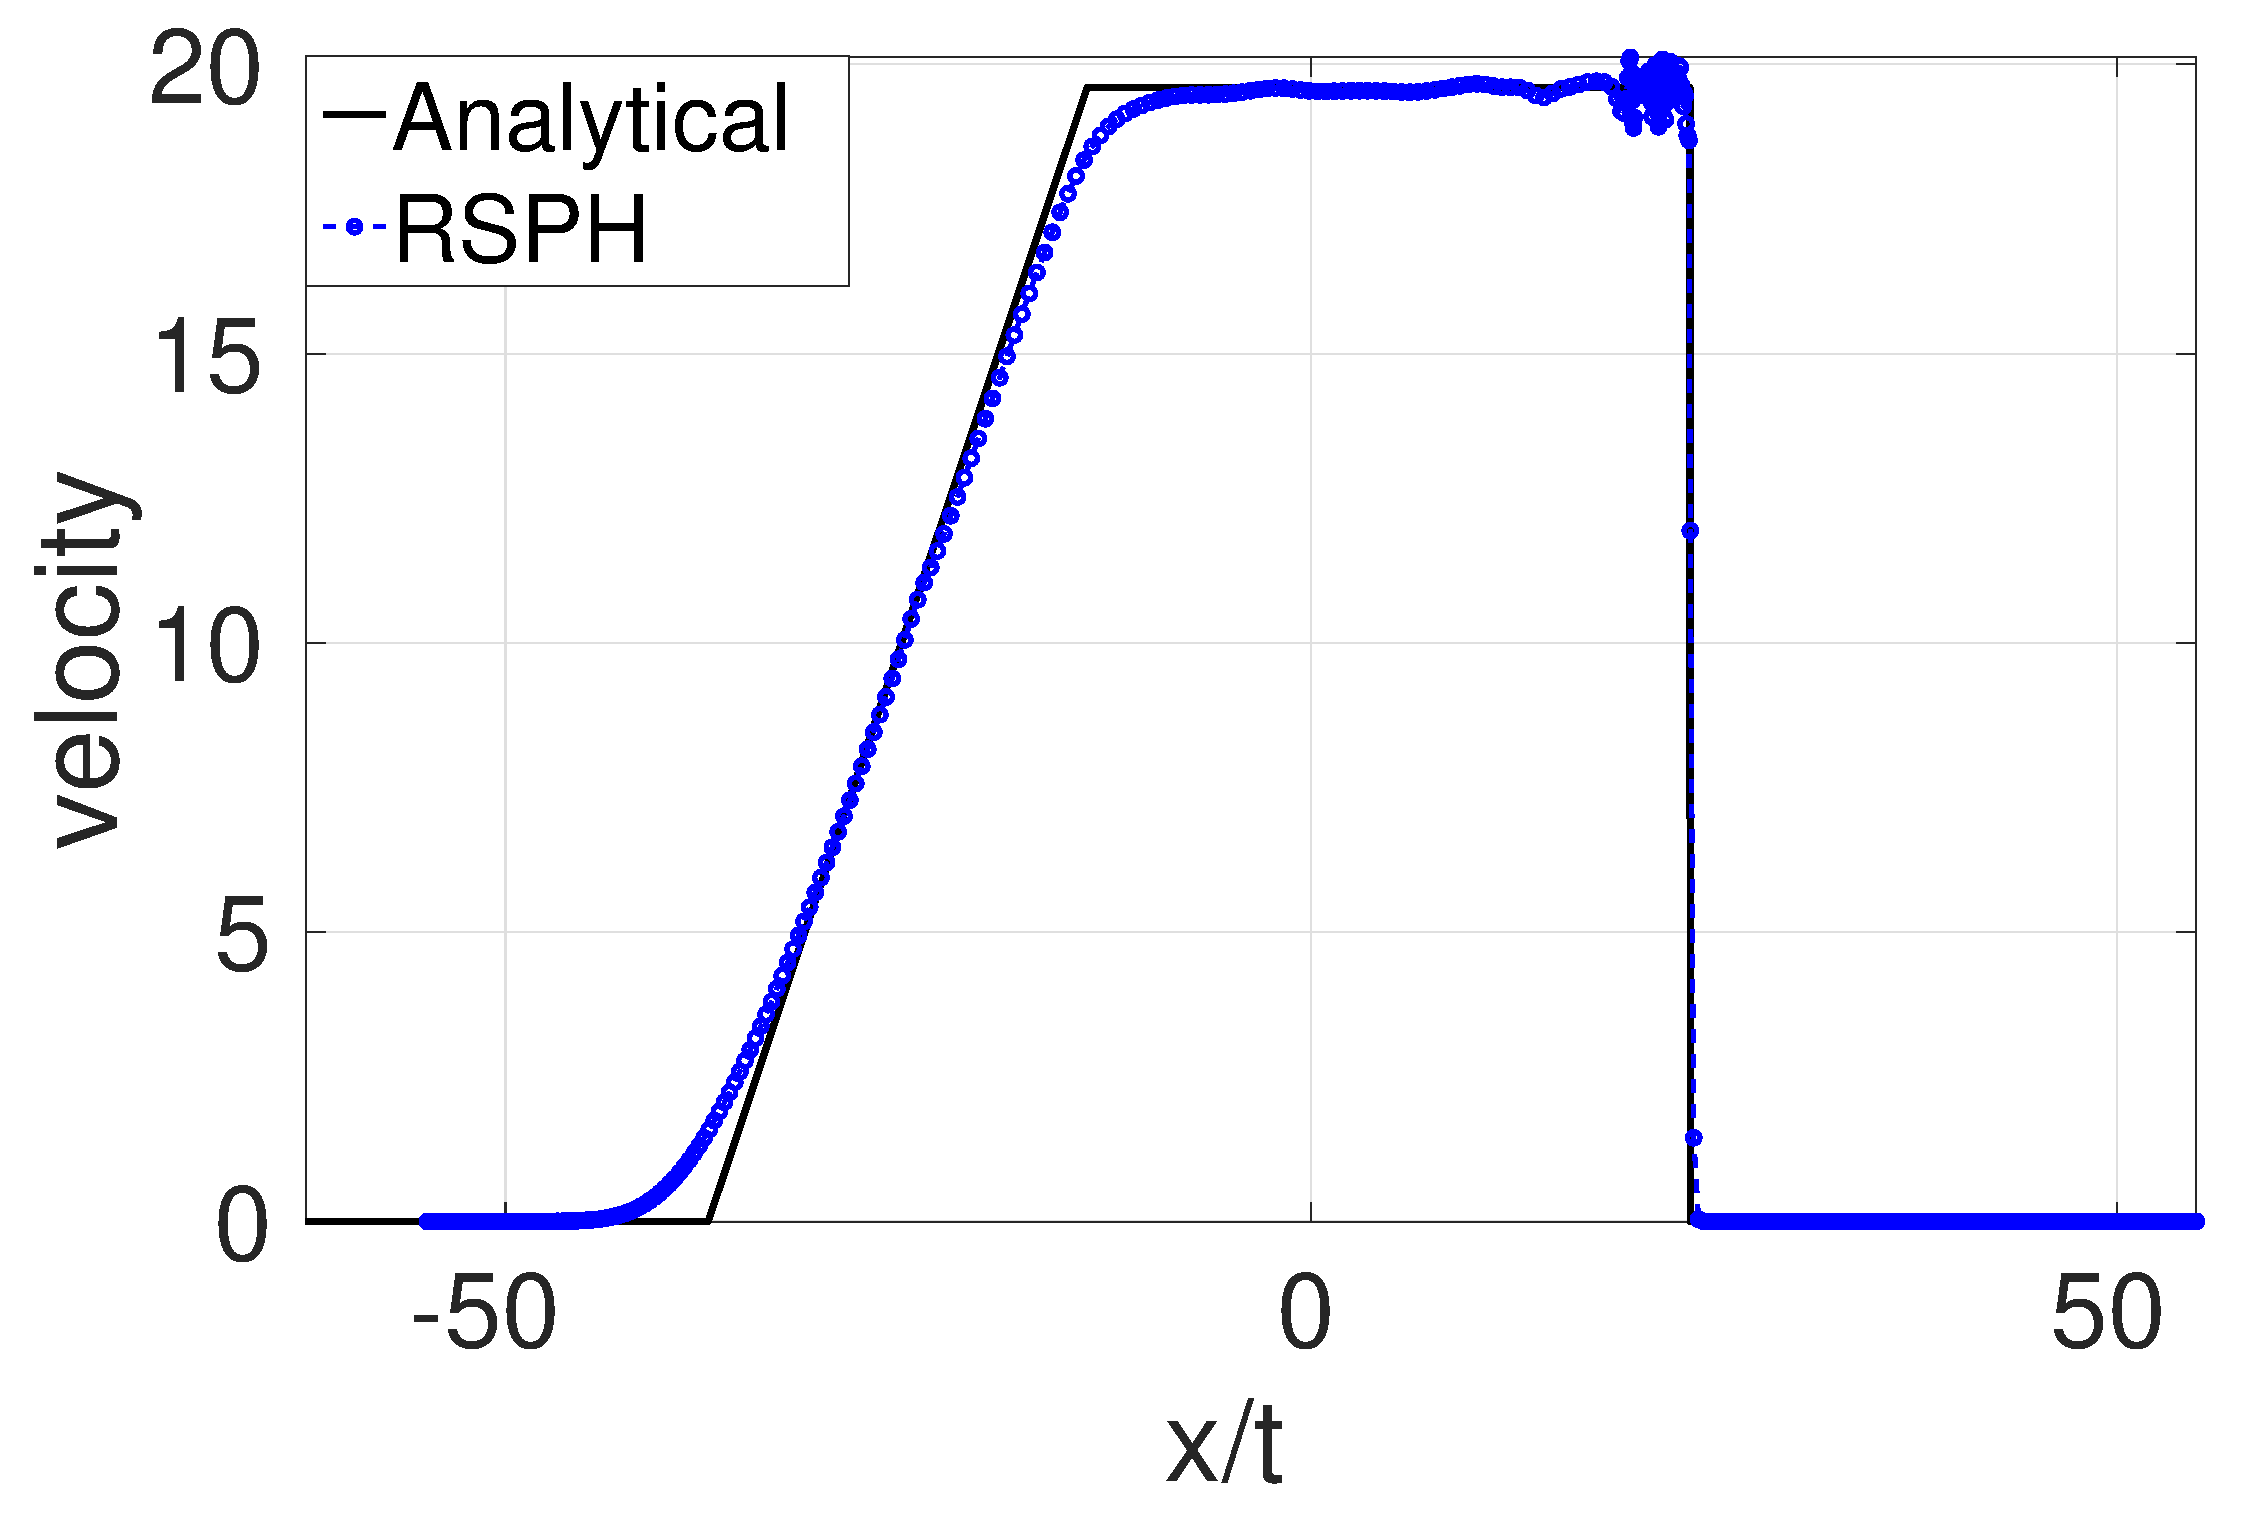
\includegraphics[width=0.99 \textwidth]{./Figures/strong-blast/StrBlst-RCM-v-Rp3}
    \end{minipage}%
    \\
    \begin{minipage}{.495 \textwidth}
        \centering
        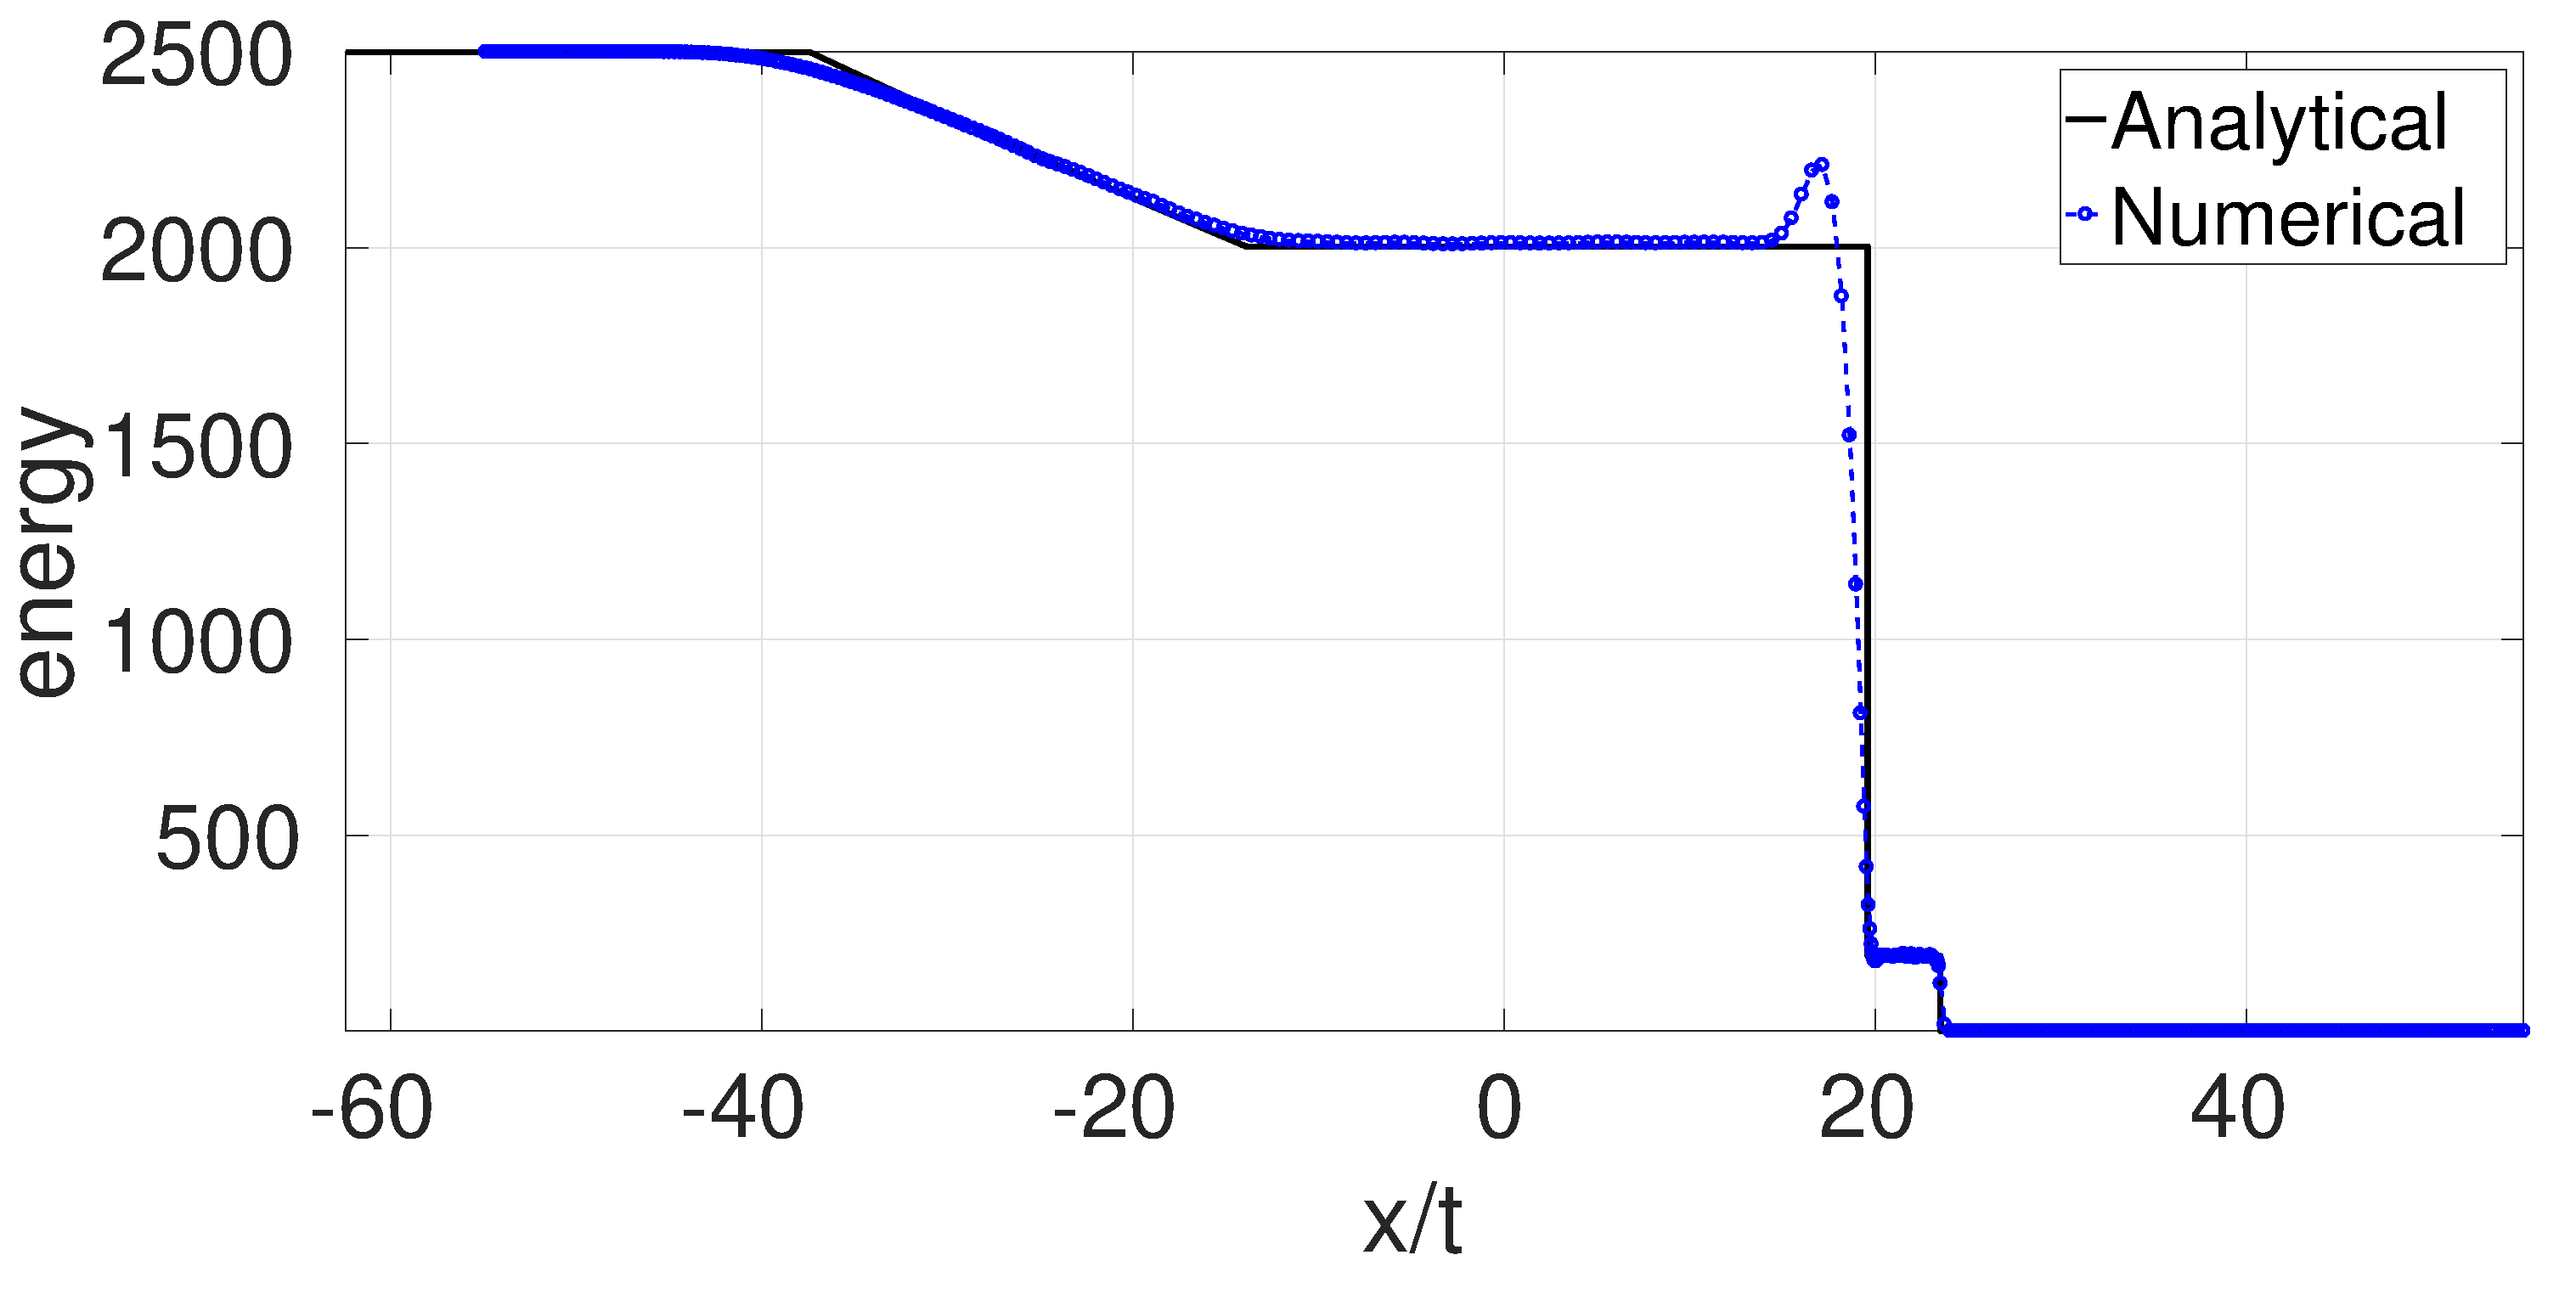
\includegraphics[width=0.99 \textwidth]{./Figures/strong-blast/StrBlst-RCM-e-Rp3}
    \end{minipage}%
    \begin{minipage}{.495 \textwidth}
        \centering
        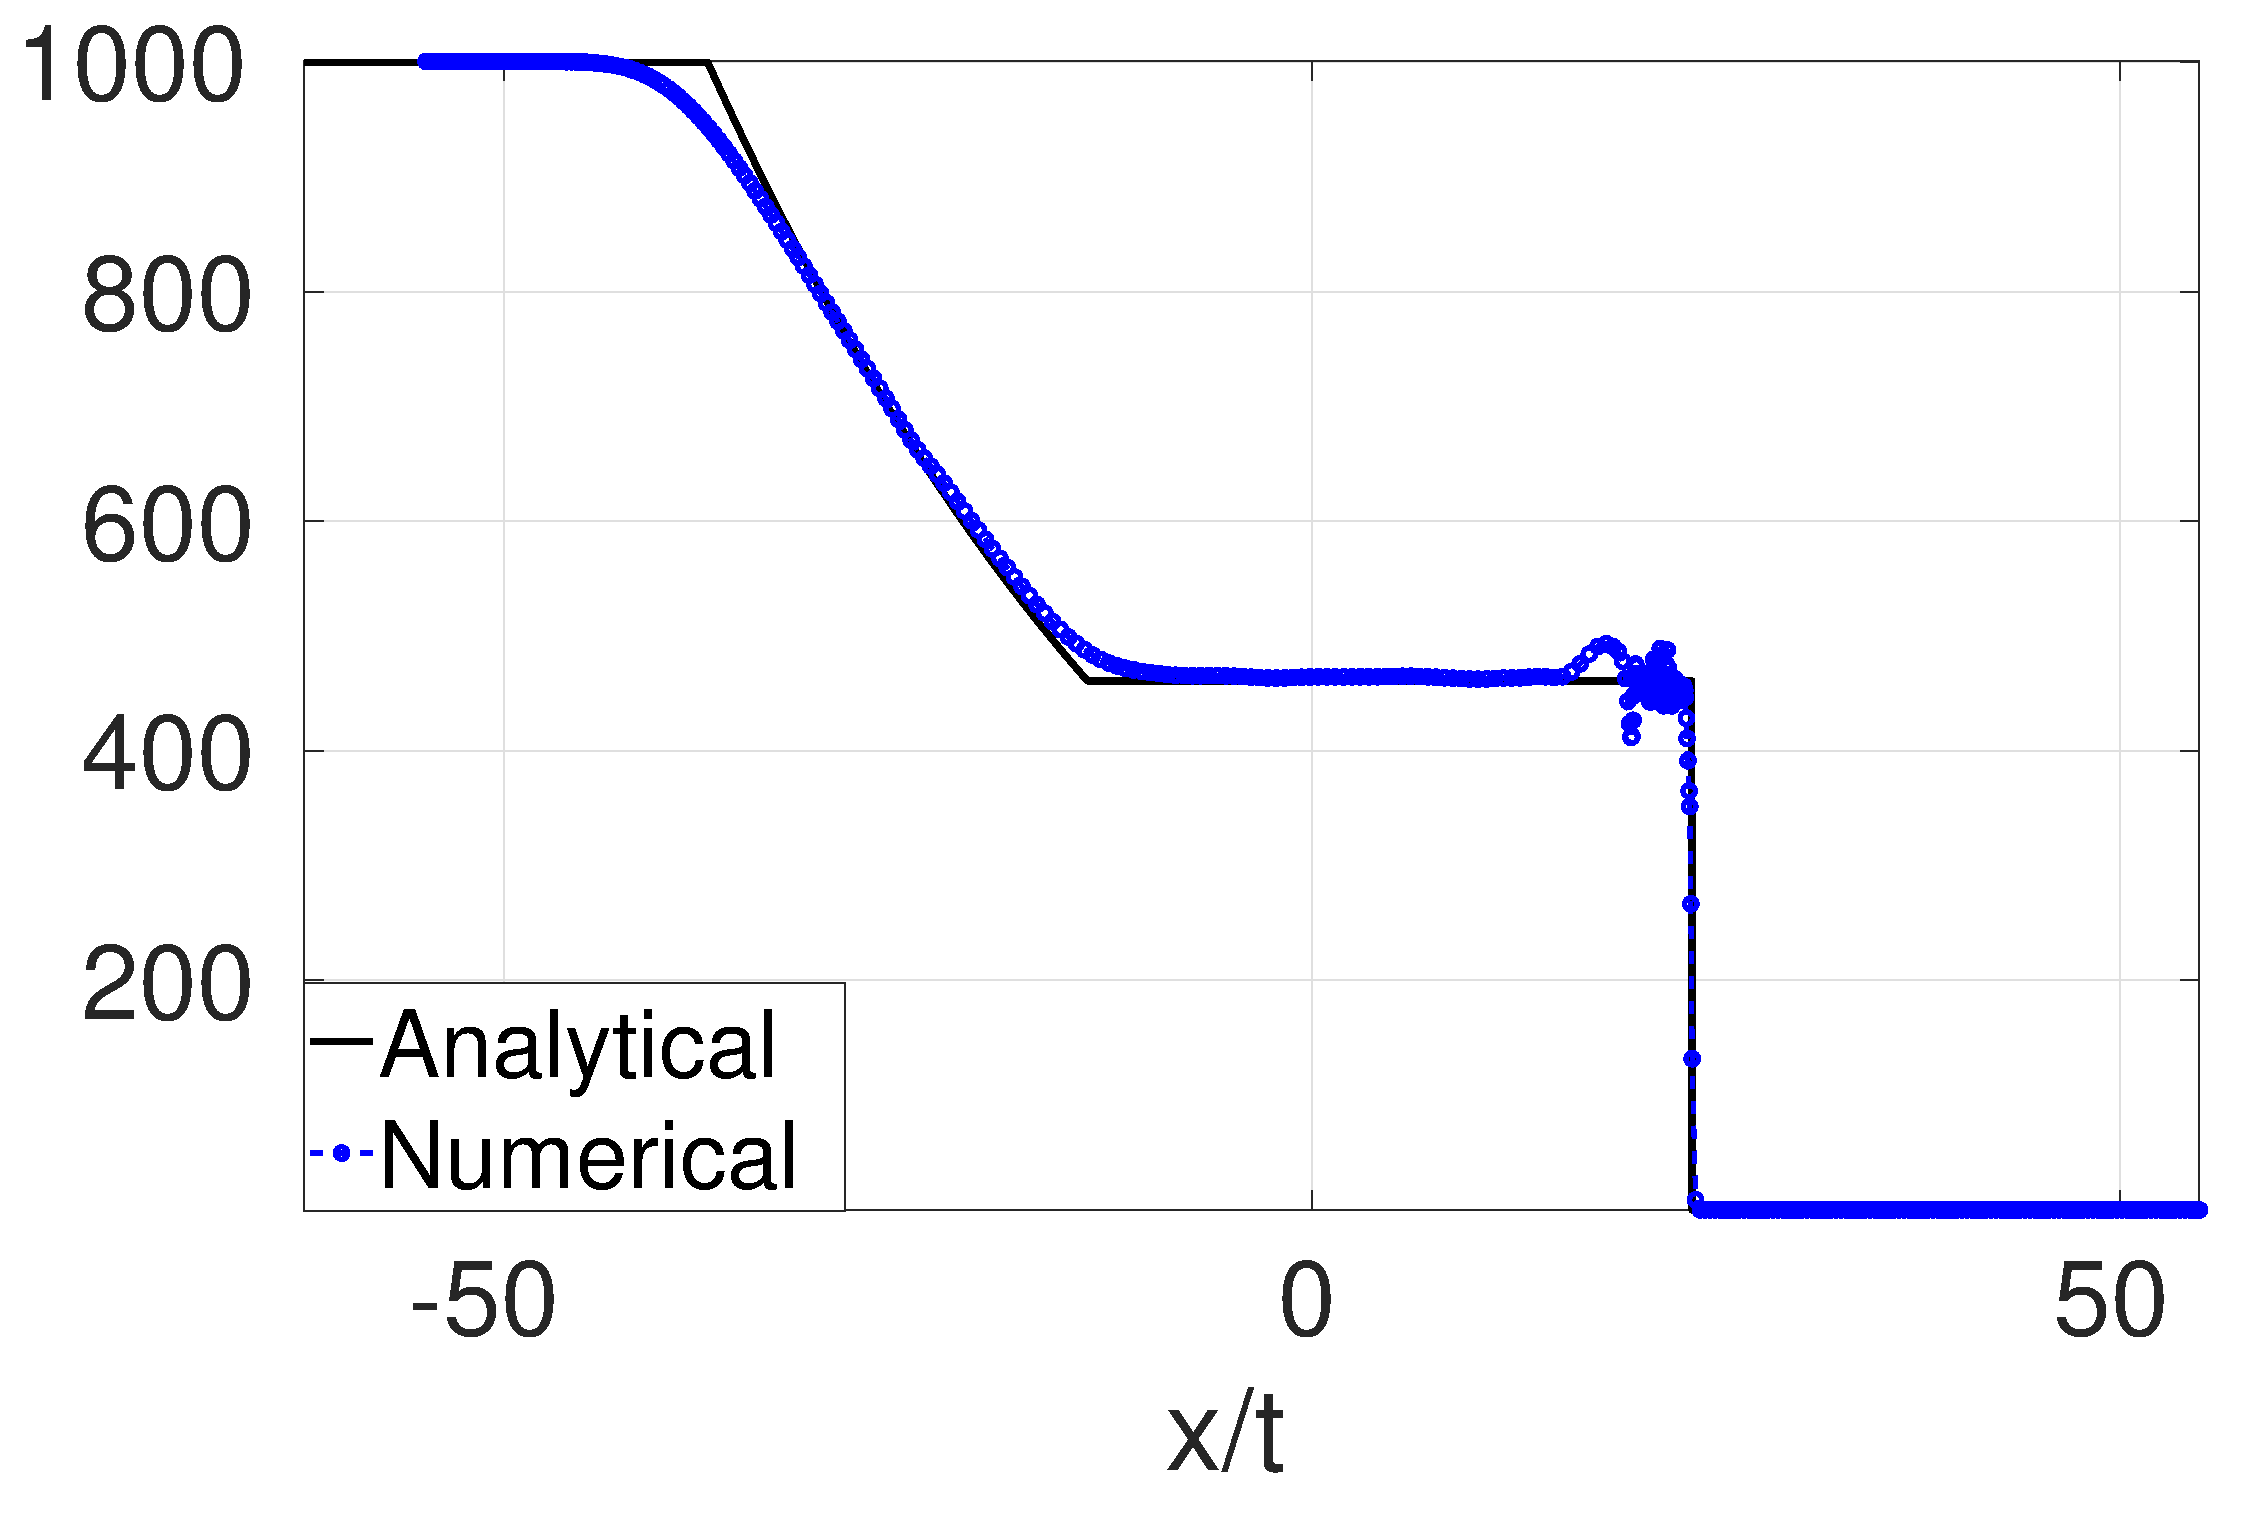
\includegraphics[width=0.99 \textwidth]{./Figures/strong-blast/StrBlst-RCM-p-Rp3}
    \end{minipage}% 
    \caption{Results for test 6, the strong blast test. y axis for density plot is in log base 10. All physical properties are well re-produced. The oscillations between shock and contact discontinuity is relatively larger than other area. A noticeable spike is observed near contact discontinuity.}
    \label{fig:RCM-strong-blast}
\end{figure}

\subsection{3D free jet}
Free jet flow have been studied analytically, experimentally and numerically for many decades, not only because of its wide application but also because of its fundamental significance as a basic flow to the scientific research community. To test the capacity of RSPH for multiple dimensional applications, a free jet flow is simulated in this section by solving 3D compressible Euler Equations using standard SPH, GSPH and RSPH. 
All simulations are using the same setting-up and compared at the same physical time. In this test, RSPH simulation is carried out based on piece wise constant construction of Riemann problem and a HLLC approximate Riemann solver. To do a well-controlled comparison, GSPH adopts the same way for Riemann problem construction and the same Riemann solver as RSPH. 

The computational domain in this test is a box. The boundaries can be categorized into the velocity inlet (a circular area at the center of the bottom of the box), non-slip wall boundary (box bottom) and pressure outlet (other faces of the box). The boundaries are set away from vent to avoid boundary effects on simulation.
At the vent, exit velocity $\textbf{v}$ is set to $500 m / s$ and radius of the nozzle $r$ is set to $8m $. The pressure of ejected fluid are assumed to be the same as ambient ($101 kpa$). The temperature of and ambient fluids are set to $273 K$. 
Velocity is zero for non-slip wall boundary. The heat flux across wall boundary is zero assuming adiabatic wall. The flux of mass should also be zero on the wall. As a result, internal energy flux, which consists of heat flux and energy flux carried by mass flux, vanishes on the wall boundary. 
The pressure of the surrounding ambient is given. As we ignore the viscosity, the shear stress is ignored and normal stress (whose magnitude equals to pressure) balances the ambient pressure.
\begin{equation}
p = p_a\left(z\right)  \label{eq:pressure_bc_p} 
\end{equation} 
Except for the pressure, boundary values for density, velocity, and energy on the outlet are determined by solution. Fluids properties of ideal gas are used in this simulation.

\begin{figure}[H]
    \centering
    \begin{minipage}[t]{.325\textwidth}
        \centering
        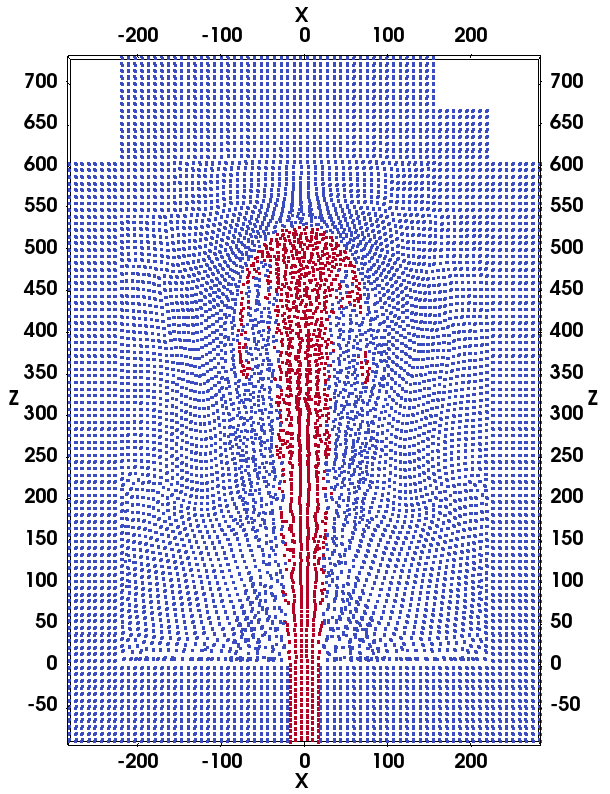
\includegraphics[width=0.99 \textwidth]{./Figures/SPH-alf2-t3-cutView}
    \end{minipage}%
    \begin{minipage}[t]{.325 \textwidth}
        \centering
        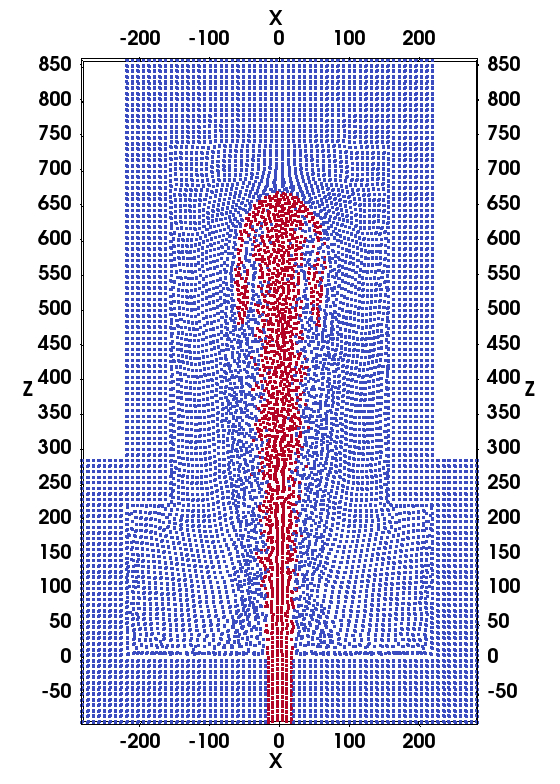
\includegraphics[width=0.99 \textwidth]{./Figures/SPH-alf1-t3-cutView}
    \end{minipage}%
    \begin{minipage}[t]{.325\textwidth}
        \centering
        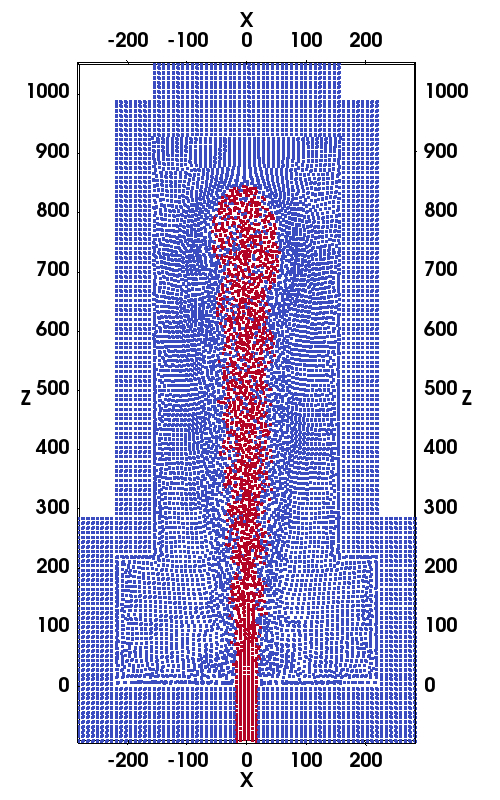
\includegraphics[width=0.99 \textwidth]{./Figures/SPH-alfp3-t3-cutView}
    \end{minipage}%
    \caption{Free jet flow simulation results at $t=3.0 s$ by SPH using different artificial viscosity coefficients. These pictures are front view of a slice of the domain cut by two planes parallel to $x-z$ plane at $y=-9$ and $y=9$. From left to right, the picture is corresponding to $\alpha=0.3$, $\alpha=1.0$ and $\alpha=2.0$ respectively. Another artificial viscosity coefficient $\beta$ is set to be double of $\alpha$ for all tests. Red particles in pictures are particles erupted from the nozzle while blues are ambient fluids particles.}
    \label{fig:free-jet-SPH-comparison}
\end{figure}

\begin{figure}[!ht]
    \centering
    \begin{minipage}[t]{.325\textwidth}
        \centering
        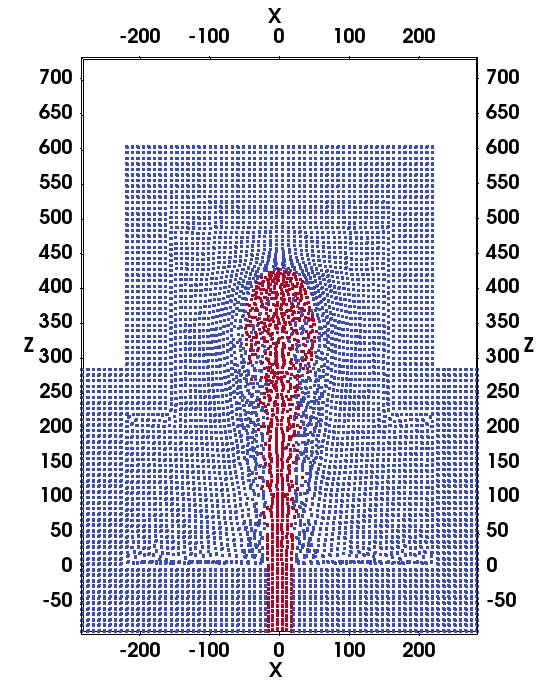
\includegraphics[width=0.99 \textwidth]{./Figures/SPH-alf1-t1p5-cutView}
    \end{minipage}%
    \begin{minipage}[t]{.325 \textwidth}
        \centering
        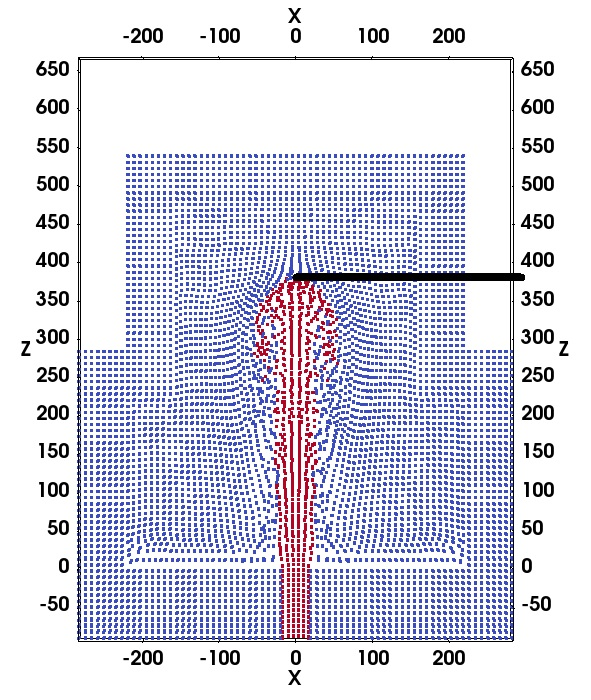
\includegraphics[width=0.99 \textwidth]{./Figures/GSPH-HLLC-t1p5-cutView}
    \end{minipage}%
    \begin{minipage}[t]{.325\textwidth}
        \centering
        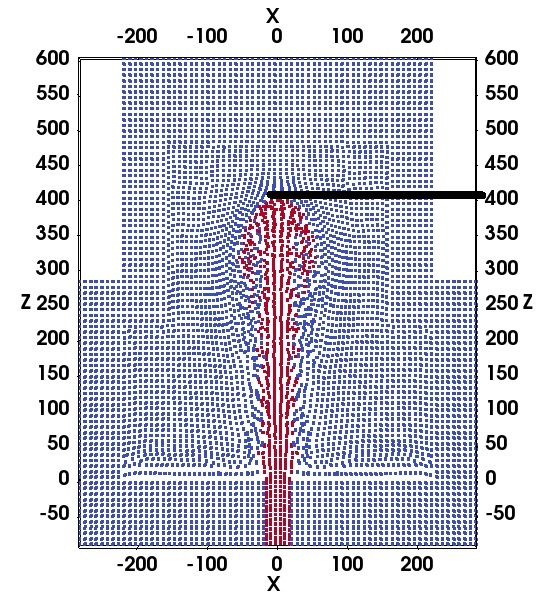
\includegraphics[width=0.99 \textwidth]{./Figures/RSPH-t1p5-cutView}
    \end{minipage}%
    \\
    \centering
    \begin{minipage}[t]{.325\textwidth}
        \centering
        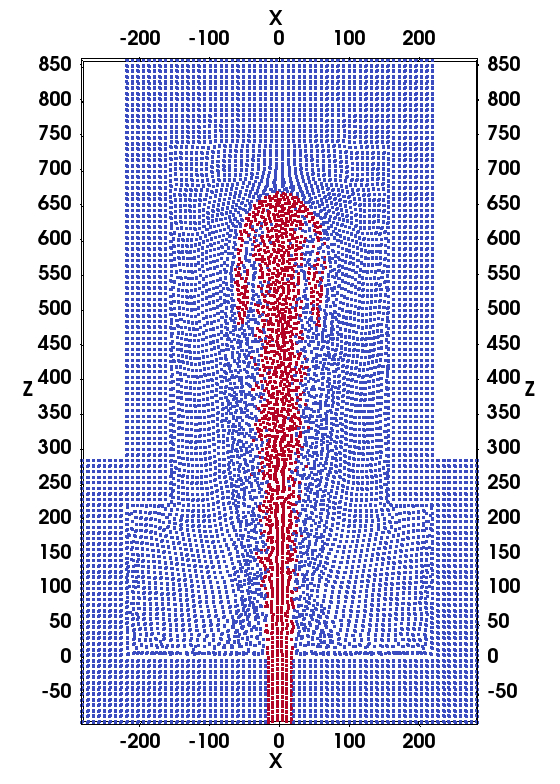
\includegraphics[width=0.99 \textwidth]{./Figures/SPH-alf1-t3-cutView}
    \end{minipage}%
    \begin{minipage}[t]{.325 \textwidth}
        \centering
        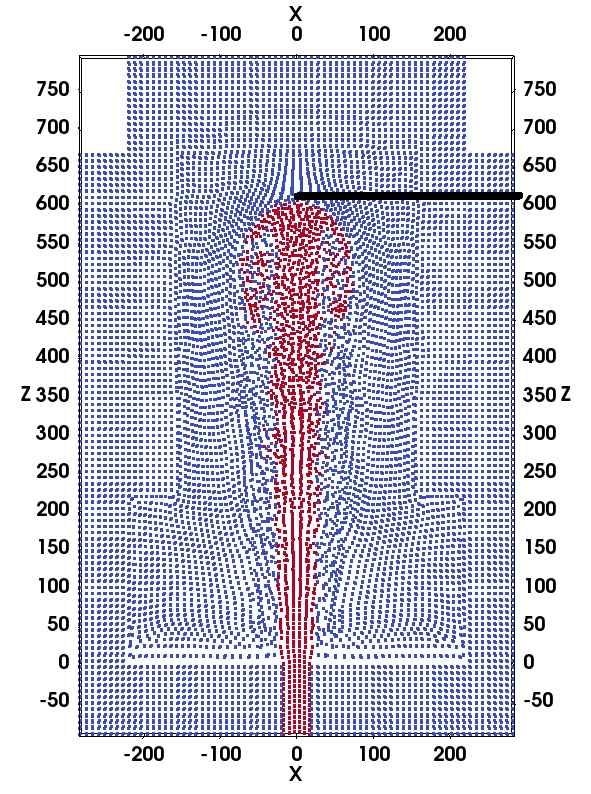
\includegraphics[width=0.99 \textwidth]{./Figures/GSPH-HLLC-t3-cutView}
    \end{minipage}%
    \begin{minipage}[t]{.325\textwidth}
        \centering
        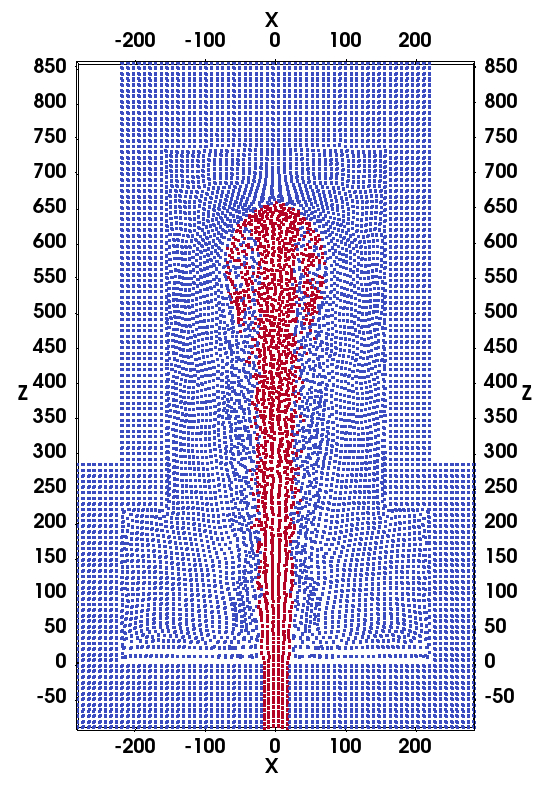
\includegraphics[width=0.99 \textwidth]{./Figures/RSPH-t3-cutView}
    \end{minipage}%
    \caption{Simulation results of free jet flow by SPH with $\alpha=1.0, \beta=2.0$, GSPH and RSPH. These pictures are front view of a slice of the domain cut by two planes parallel to $x-z$ plane at $y=-9$ and $y=9$. From left to right, the picture is corresponding to SPH, GSPH and RSPH respectively. Red particles in pictures of the first row are particles erupted from the nozzle while blues are ambient fluids particles. Pictures on the first row are corresponding to $t=1.5s$ while pictures on the second row are for $t=3.0 s$}
    \label{fig:free-jet-comparison}
\end{figure}

Figure \ref{fig:free-jet-SPH-comparison} shows simulation results of the free jet flow by SPH with different artificial viscosity coefficients. The damping effect due to artificial dissipation is clearly shown in this figure. We observe that the lengths to which these jets reach at $t=3.0 s$ are various when using different artificial viscosity coefficient. It is obvious that the larger artificial viscosity, the shorter length the jet can reach. While introducing undesirable damping effects, artificial viscosity is necessary for numerical stability and simulating of shocks. So, in real applications, the artificial viscosity coefficients are usually tuned (see, for example, \citep{gmd-2017-119}) to avoid excessive artificial damping effects.

We compare RSPH with GSPH in terms of equivalent overall artificial damping effects. Different from SPH, both GSPH and RSPH introduce artificial viscosity in an implicit way by solving local Riemann problems. As has been shown in 1D tests, RSPH can introduce less artificial viscosity than GSPH. Fig. \ref{fig:free-jet-comparison} implies that RSPH introduces less overall damping effect than GSPH in 3D application as well, which is consistent with 1D tests. That is to say, RSPH's desirable property of introducing less artificial dissipation in 1D unsteady flow is inherited in 3D applications of RSPH. Recall that RCM shows ability of resolving discontinuities as true discontinuities in 1D unsteady flows but such very desirable property does not persist in genuine two (or higher) space dimensions \citep{colella1982glimm}. Integrating of RCM within the framework of SPH avoids solving higher dimensional Riemann problems overcoming the fundamental shortcoming of RCM.

\section{Conclusion}
We proposed RSPH, a novel SPH scheme for solving hyperbolic non-linear PDEs. The artificial viscosity in RSPH is determined implicitly by randomly sampling solution of a local Riemann problem. No explicit artificial viscosity coefficients is needed. The artificial viscosity introduced by RSPH is demonstrated to be much less than GSPH and SPH without parameter tuning. Besides introducing less amount of dissipation, there are several other attractive features. The pressure ``wiggle" around contact discontinuity, which persists in SPH results, is eliminated in RSPH. It also shows higher order of convergence rate than GSPH when the same construction of local Riemann problem and Riemann solvers. The attractive property of less dissipation persist in multi-dimensional applications.
This new method enables shock capturing with lower dissipation. One potential application of the method is high speed mixing flow, for example, supersonic combustion.
By overcoming a fundamental shortcoming of RCM and inheriting attractive feature of RCM, RSPH provide a powerful numerical method for solving combustion problems in multi-dimensional space.

One shortcoming of RSPH is its inability to completely suppress numerical perturbation caused by non-uniform distribution of smoothing length in space. Such perturbation, as long as it does not lead to numerical instability, is within acceptable range for many tests. However, for very strong shocks, dissipation introduced by RSPH turns out to be not sufficient to stabilize simulation, which finally ends up with negative energy. Since GSPH has been shown introducing more dissipation and hence is more suitable for situation with very strong shocks.

In our investigation presented in this paper, an approximate HLLC Riemann solver is used in place of exact iterative Riemann solver. It would be interesting to see the difference, between using other approximate Riemann solvers and exact Riemann solver. Alternative Riemann solvers, alternative ways for constructing Riemann problems and alternative ways for sampling solution of Riemann problem might also worthwhile for future exploring. In addition, this paper focused on solving of compressible Euler equations. Applications of RSPH in other computational fluids dynamic problems or solving other hyperbolic PDEs are on the list to be explored.

\section*{acknowledgements}
3D simulations reported here were performed at the Center for Computational Research (CCR) at the University at Buffalo. This project is supported by Grants No. NSF ACI/1131074 from the National Science Foundation.

\section*{References}
\bibliography{Reference}
\end{document}
